%        File: arfc-beamer.tex
%     Created: Sun May 5 10:00 PM 2013 C


%\documentclass[11pt,handout]{beamer}
\documentclass[8pt]{beamer}
\usetheme[white]{Illinois}
%\title[short title]{long title}
\title[Moltres Advancement]{Advancements in Moltres for Time-Dependent Multiphysics Molten Salt
Reactor Modeling}
%\subtitle[short subtitle]{long subtitle}
\subtitle[Final]{Final Examination}
%\subtitle[Brief Summary]{A Brief Summary}
%\author[short name]{long name}
\author[Authors]{Sun Myung Park\\Advanced Reactors and Fuel Cycles Group}
%\date[short date]{long date}
\date[12.12.2024]{December 12, 2024}
%\institution[short name]{long name}
\institute{
  Nuclear, Plasma \& Radiological Engineering\\University of
Illinois Urbana-Champaign}

%\usepackage{bbding}
\usepackage{amsfonts}
\usepackage{amsmath}
\usepackage{amssymb}
\usepackage{mathtools}
\usepackage{bm}
\usepackage{stmaryrd}
\usepackage{xspace}
\usepackage{xcolor}
\usepackage{graphicx}
\graphicspath{{../images/}}
\usepackage{subcaption}
\usepackage{multirow}
\usepackage{siunitx}
\usepackage{booktabs} % nice rules for tables
\usepackage{colortbl}
\usepackage{microtype} % if using PDF
\usepackage{bigints}
\usepackage{minted}
\usepackage[absolute,overlay]{textpos}
\usepackage{tikz}
\usepackage{tkz-euclide}
\usetikzlibrary{positioning, arrows, decorations, shapes, fit, backgrounds}
\usetikzlibrary{shapes.geometric,arrows}
\definecolor{illiniblue}{HTML}{B1C6E2}
\definecolor{illiniorange}{HTML}{f8c2a2}
\definecolor{green}{HTML}{c2e2b1}
\tikzstyle{process} = [rectangle, rounded corners, thick, minimum width=7cm, minimum height=1cm, text centered, draw=black, fill=illiniblue, text width=18em]
\tikzstyle{object} = [ellipse, minimum width=2cm, thick, minimum height=2.2cm, text centered, draw=black, fill=illiniorange, text width=12em]
\tikzstyle{decision} = [diamond, thick, aspect=2, minimum width=2cm, minimum height=2cm, text centered, draw=black, fill=green, text width=6em]
\tikzstyle{arrow} = [thick,->,>=stealth]
\tikzstyle{solver} = [rectangle, rounded corners, thick, minimum width=3cm, minimum height=1.5cm, text centered, draw=black, fill=illiniblue, text width=7em]
\tikzstyle{bound} = [rectangle, rounded corners, thick, draw=black]
\tikzstyle{solver2} = [rectangle, rounded corners, thick, minimum width=2cm, minimum height=1cm, text centered, draw=black, fill=illiniblue, text width=5em]
\tikzstyle{bound} = [rectangle, rounded corners, thick, draw=black]

\usepackage[utf8]{inputenc}
\usepackage[english]{babel}
\usepackage[bibstyle=ieee,backend=bibtex8,sorting=none,eprint=false,isbn=false,doi=false]{biblatex}
\usepackage{textalpha}
\addbibresource{../bibliography.bib}
\AtEveryBibitem{%
  \clearfield{note}%
}
\renewcommand*{\bibfont}{\tiny}

\newcommand{\units}[1] {\:\text{#1}}%
\newcommand{\SN}{S$_N$}%{S$_\text{N}$}%{$S_N$}%
\DeclareMathOperator{\erf}{erf}
%I need some complimentary error functions... 
\DeclareMathOperator{\erfc}{erfc}
%Those icons in the references are terrible looking
\setbeamertemplate{bibliography item}[text]
%Figure numbering
\setbeamertemplate{caption}[numbered]
\setbeamerfont{caption}{size=\small}

%%%% Acronym support

\usepackage[acronym,toc]{glossaries}
%\newacronym{<++>}{<++>}{<++>}
\newacronym[longplural={metric tons of heavy metal}]{MTHM}{MTHM}{metric ton of heavy metal}
\newacronym{ABM}{ABM}{agent-based modeling}
\newacronym{ACDIS}{ACDIS}{Program in Arms Control \& Domestic and International Security}
\newacronym{AEF}{AEF}{Averaged Eddington Factor}
\newacronym{AHTR}{AHTR}{Advanced High Temperature Reactor}
\newacronym{ANDRA}{ANDRA}{Agence Nationale pour la gestion des D\'echets RAdioactifs, the French National Agency for Radioactive Waste Management}
\newacronym{ANL}{ANL}{Argonne National Laboratory}
\newacronym{API}{API}{application programming interface}
\newacronym{ARDP}{ARDP}{Advanced Reactor Demonstration Program}
\newacronym{ARE}{ARE}{Aircraft Reactor Experiment}
\newacronym{ASME}{ASME}{American Society of Mechanical Engineers}
\newacronym{ATWS}{ATWS}{Anticipated Transient Without Scram}
\newacronym{BDBE}{BDBE}{Beyond Design Basis Event}
\newacronym{BIDS}{BIDS}{Berkeley Institute for Data Science}
\newacronym{BTE}{BTE}{Boltzmann transport equation}
\newacronym{BWR}{BWR}{boiling water reactor}
\newacronym{CAFCA}{CAFCA}{ Code for Advanced Fuel Cycles Assessment }
\newacronym{CAS}{CAS}{Chinese Academy of Sciences}
\newacronym{CDTN}{CDTN}{Centro de Desenvolvimento da Tecnologia Nuclear}
\newacronym{CEA}{CEA}{Commissariat \`a l'\'Energie Atomique et aux \'Energies Alternatives}
\newacronym{CFD}{CFD}{Computational Fluid Dynamics}
\newacronym{CI}{CI}{continuous integration}
\newacronym{CNEN}{CNEN}{Comiss\~{a}o Nacional de Energia Nuclear}
\newacronym{CNERG}{CNERG}{Computational Nuclear Engineering Research Group}
\newacronym{CNRS}{CNRS}{Centre National de la Recherche Scientifique}
\newacronym{COMSOL}{COMSOL}{COMmon SOLution}
\newacronym{COSI}{COSI}{Commelini-Sicard}
\newacronym{COTS}{COTS}{commercial, off-the-shelf}
\newacronym{CPM}{CPM}{collision probability method}
\newacronym{CSNF}{CSNF}{commercial spent nuclear fuel}
\newacronym{CTAH}{CTAHs}{Coiled Tube Air Heaters}
\newacronym{CUBIT}{CUBIT}{CUBIT Geometry and Mesh Generation Toolkit}
\newacronym{CURIE}{CURIE}{Centralized Used Fuel Resource for Information Exchange}
\newacronym{DAG}{DAG}{directed acyclic graph}
\newacronym{DANESS}{DANESS}{Dynamic Analysis of Nuclear Energy System Strategies}
\newacronym{DBE}{DBE}{Design Basis Event}
\newacronym{DES}{DES}{Detached eddy simulation}
\newacronym{DESAE}{DESAE}{Dynamic Analysis of Nuclear Energy Systems Strategies}
\newacronym{DF}{DF}{discontinuity factors}
\newacronym{DFEM}{DFEM}{discontinuous finite element method}
\newacronym{DG}{DG}{Discontinuous Galerkin}
\newacronym{DHS}{DHS}{Department of Homeland Security}
\newacronym{DNF}{DNF}{delayed neutron fraction}
\newacronym{DNP}{DNP}{delayed neutron precursor}
\newacronym{DNS}{DNS}{Direct numerical simulation}
\newacronym{DOE}{DOE}{Department of Energy}
\newacronym{DMSR}{DMSR}{Denatured Molten Salt Reactor}
\newacronym{DRACS}{DRACS}{Direct Reactor Auxiliary Cooling System}
\newacronym{DRE}{DRE}{dynamic resource exchange}
\newacronym{DSNF}{DSNF}{DOE spent nuclear fuel}
\newacronym{DYMOND}{DYMOND}{Dynamic Model of Nuclear Development }
\newacronym{EBS}{EBS}{Engineered Barrier System}
\newacronym{EDZ}{EDZ}{Excavation Disturbed Zone}
\newacronym{EPA}{EPA}{Environmental Protection Agency}
\newacronym{EP}{EP}{Engineering Physics}
\newacronym{EVOL}{EVOL}{Evaluation and Viability of Liquid Fuel Fast Reactor System}
\newacronym{FCO}{FCO}{Fuel Cycle Options}
\newacronym{FCT}{FCT}{Fuel Cycle Technology}
\newacronym{FEHM}{FEHM}{Finite Element Heat and Mass Transfer}
\newacronym{FEM}{FEM}{finite element method}
\newacronym{FEPs}{FEPs}{Features, Events, and Processes}
\newacronym{FHR}{FHR}{Fluoride-Salt-Cooled High-Temperature Reactor}
\newacronym{FLiBe}{FLiBe}{Fluoride-Lithium-Beryllium}
\newacronym{FP}{FP}{fission product}
\newacronym{FVM}{FVM}{finite volume method}
\newacronym{GDSE}{GDSE}{Generic Disposal System Environment}
\newacronym{GDSM}{GDSM}{Generic Disposal System Model}
\newacronym{GENIUSv1}{GENIUSv1}{Global Evaluation of Nuclear Infrastructure Utilization Scenarios, Version 1}
\newacronym{GENIUSv2}{GENIUSv2}{Global Evaluation of Nuclear Infrastructure Utilization Scenarios, Version 2}
\newacronym{GENIUS}{GENIUS}{Global Evaluation of Nuclear Infrastructure Utilization Scenarios}
\newacronym{GET}{GET}{general equivalence theory}
\newacronym{GIF}{GIF}{Generation IV International Forum}
\newacronym{GPAM}{GPAM}{Generic Performance Assessment Model}
\newacronym{GRSAC}{GRSAC}{Graphite Reactor Severe Accident Code}
\newacronym{GUI}{GUI}{graphical user interface}
\newacronym{HALEU}{HALEU}{high-assay low-enriched uranium}
\newacronym{HLW}{HLW}{high level waste}
\newacronym{HPC}{HPC}{high-performance computing}
\newacronym{HTC}{HTC}{high-throughput computing}
\newacronym{HTGR}{HTGR}{High-Temperature Gas-Cooled Reactor}
\newacronym{IAEA}{IAEA}{International Atomic Energy Agency}
\newacronym{IDT}{IDT}{integrated diffusion/transport}
\newacronym{IEA}{IEA}{International Energy Agency}
\newacronym{IEMA}{IEMA}{Illinois Emergency Mangament Agency}
\newacronym{IHLRWM}{IHLRWM}{International High Level Radioactive Waste Management}
\newacronym{IMSBR}{IMSBR}{Indian Molten Salt Breeder Reactor}
\newacronym{IMSR}{IMSR}{Integral Molten Salt Reactor}
\newacronym{INL}{INL}{Idaho National Laboratory}
\newacronym{INS}{INS}{incompressible Navier-Stokes}
\newacronym{IO}{I/O}{input/output}
\newacronym{IPRR1}{IRP-R1}{Instituto de Pesquisas Radioativas Reator 1}
\newacronym{IRP}{IRP}{Integrated Research Project}
\newacronym{IRPhEP}{IRPhEP}{International Reactor Physics Benchmark Experiment Evaluation Project}
\newacronym{ISFSI}{ISFSI}{Independent Spent Fuel Storage Installation}
\newacronym{ISRG}{ISRG}{Independent Student Research Group}
\newacronym{JFNK}{JFNK}{Jacobian-Free Newton Krylov}
\newacronym{LANL}{LANL}{Los Alamos National Laboratory}
\newacronym{LBNL}{LBNL}{Lawrence Berkeley National Laboratory}
\newacronym{LCOE}{LCOE}{levelized cost of electricity}
\newacronym{LDRD}{LDRD}{laboratory directed research and development}
\newacronym{LES}{LES}{Large eddy simulation}
\newacronym{LEU}{LEU}{low-enriched uranium}
\newacronym{LFR}{LFR}{Lead-Cooled Fast Reactor}
\newacronym{LFMSR}{LFMSR}{Liquid-fueled Molten Salt Reactor}
\newacronym{LGPL}{LGPL}{GNU Lesser General Public License}
\newacronym{LLNL}{LLNL}{Lawrence Livermore National Laboratory}
\newacronym{LMFBR}{LMFBR}{Liquid Metal Fast Breeder Reactor}
\newacronym{LOFC}{LOFC}{Loss of Forced Cooling}
\newacronym{LOHS}{LOHS}{Loss of Heat Sink}
\newacronym{LOLA}{LOLA}{Loss of Large Area}
\newacronym{LP}{LP}{linear program}
\newacronym{LWR}{LWR}{Light Water Reactor}
\newacronym{MAGNOX}{MAGNOX}{Magnesium Alloy Graphie Moderated Gas Cooled Uranium Oxide Reactor}
\newacronym{MA}{MA}{minor actinide}
\newacronym{MCFR}{MCFR}{Molten Chloride Fast Reactor}
\newacronym{MCNP}{MCNP}{Monte Carlo N-Particle code}
\newacronym{MCRE}{MCRE}{Molten Chloride Reactor Experiment}
\newacronym{MECS}{MECS}{Method of Equivalent Cross Sections}
\newacronym{MILP}{MILP}{mixed-integer linear program}
\newacronym{MIT}{MIT}{the Massachusetts Institute of Technology}
\newacronym{MOAB}{MOAB}{Mesh-Oriented datABase}
\newacronym{MOOSE}{MOOSE}{Multiphysics Object-Oriented Simulation Environment}
\newacronym{MOSART}{MOSART}{Molten Salt Actinide Recycler and Transmuter}
\newacronym{MOX}{MOX}{mixed oxide}
\newacronym{MPI}{MPI}{Message Passing Interface}
\newacronym{MPM}{MPM}{Multi-Physics Modelling}
\newacronym{MRPP}{MRPP}{Multiregion Processing Plant}
\newacronym{MSBR}{MSBR}{Molten Salt Breeder Reactor}
\newacronym{MSFR}{MSFR}{Molten Salt Fast Reactor}
\newacronym{MSRE}{MSRE}{Molten Salt Reactor Experiment}
\newacronym{MSR}{MSR}{Molten Salt Reactor}
\newacronym{NAGRA}{NAGRA}{National Cooperative for the Disposal of Radioactive Waste}
\newacronym{NEAMS}{NEAMS}{Nuclear Energy Advanced Modeling and Simulation}
\newacronym{NEUP}{NEUP}{Nuclear Energy University Programs}
\newacronym{NFCSim}{NFCSim}{Nuclear Fuel Cycle Simulator}
\newacronym{NGNP}{NGNP}{Next Generation Nuclear Plant}
\newacronym{NMWPC}{NMWPC}{Nuclear MW Per Capita}
\newacronym{NNSA}{NNSA}{National Nuclear Security Administration}
\newacronym{NPP}{NPP}{Nuclear Power Plant}
\newacronym{NPRE}{NPRE}{Department of Nuclear, Plasma, and Radiological Engineering}
\newacronym{NQA1}{NQA-1}{Nuclear Quality Assurance - 1}
\newacronym{NRC}{NRC}{Nuclear Regulatory Commission}
\newacronym{NSF}{NSF}{National Science Foundation}
\newacronym{NSSC}{NSSC}{Nuclear Science and Security Consortium}
\newacronym{NUWASTE}{NUWASTE}{Nuclear Waste Assessment System for Technical Evaluation}
\newacronym{NWF}{NWF}{Nuclear Waste Fund}
\newacronym{NWTRB}{NWTRB}{Nuclear Waste Technical Review Board}
\newacronym{NZE}{NZE}{Net-Zero Emissions by 2050 Scenario}
\newacronym{OCRWM}{OCRWM}{Office of Civilian Radioactive Waste Management}
\newacronym{OOP}{OOP}{Object-oriented programming}
\newacronym{ORION}{ORION}{ORION}
\newacronym{ORNL}{ORNL}{Oak Ridge National Laboratory}
\newacronym{PARCS}{PARCS}{Purdue Advanced Reactor Core Simulator}
\newacronym{PBAHTR}{PB-AHTR}{Pebble Bed Advanced High Temperature Reactor}
\newacronym{PBFHR}{PB-FHR}{Pebble-Bed Fluoride-Salt-Cooled High-Temperature Reactor}
\newacronym{PDE}{PDE}{partial differential equation}
\newacronym{PEI}{PEI}{Peak Environmental Impact}
\newacronym{PH}{PRONGHORN}{PRONGHORN}
\newacronym{PoliMi}{PoliMi}{Politecnico di Milano}
\newacronym{PRIS}{PRIS}{Power Reactor Information System}
\newacronym{PRKE}{PRKE}{Point Reactor Kinetics Equations}
\newacronym{PSI}{PSI}{Paul Scherrer Institute}
\newacronym{PSPG}{PSPG}{Pressure-Stabilizing/Petrov-Galerkin}
\newacronym{PV}{PV}{photovoltaic}
\newacronym{PWAR}{PWAR}{Pratt and Whitney Aircraft Reactor}
\newacronym{PWR}{PWR}{Pressurized Water Reactor}
\newacronym{PyNE}{PyNE}{Python toolkit for Nuclear Engineering}
\newacronym{PyRK}{PyRK}{Python for Reactor Kinetics}
\newacronym{QA}{QA}{quality assurance}
\newacronym{QD}{QD}{quasi-diffusion}
\newacronym{RANS}{RANS}{Reynolds-averaged Navier-Stokes}
\newacronym{RDD}{RD\&D}{Research Development and Demonstration}
\newacronym{RD}{R\&D}{Research and Development}
\newacronym{REE}{REE}{rare earth element}
\newacronym{RELAP}{RELAP}{Reactor Excursion and Leak Analysis Program}
\newacronym{RIA}{RIA}{Reactivity Insertion Accident}
\newacronym{RIF}{RIF}{Region-Institution-Facility}
\newacronym{RMM}{RMM}{Response Matrix Method}
\newacronym{ROD}{ROD}{Reactor Optimum Design}
\newacronym{RSM}{RSM}{Reynolds stress model}
\newacronym{SAAF}{SAAF}{self-adjoint angular flux}
\newacronym{SAM}{SAM}{System Analysis Module}
\newacronym{SAMOFAR}{SAMOFAR}{Safety Assessment of the Molten Salt Fast Reactor}
\newacronym{SAMOSAFER}{SAMOSAFER}{Severe Accident Modeling and Safety Assessment for Fluid-fuel Energy Reactors}
\newacronym{SD}{SD}{standard deviation}
\newacronym{SFR}{SFR}{Sodium-Cooled Fast Reactor}
\newacronym{SINAP}{SINAP}{Shanghai Institute of Applied Physics}
\newacronym{SINDAG}{SINDA{\textbackslash}G}{Systems Improved Numerical Differencing Analyzer $\backslash$ Gaski}
\newacronym{SKB}{SKB}{Svensk K\"{a}rnbr\"{a}nslehantering AB}
\newacronym{SNF}{SNF}{spent nuclear fuel}
\newacronym{SNL}{SNL}{Sandia National Laboratory}
\newacronym{SPH}{SPH}{superhomogenization}
\newacronym{STC}{STC}{specific temperature change}
\newacronym{SUPG}{SUPG}{Streamline-Upwind/Petrov-Galerkin}
\newacronym{SVDC}{SVDC}{spatially varying diffusion coefficient}
\newacronym{SWF}{SWF}{Separations and Waste Forms}
\newacronym{SWU}{SWU}{Separative Work Unit}
\newacronym{TFM}{TFM}{Transient Fission Matrix}
\newacronym{TH}{TH}{thermal-hydraulics}
\newacronym{TMSR}{TMSR}{Thorium Molten Salt Reactor}
\newacronym{TRACE}{TRACE}{TRAC/RELAP Advanced Computational Engine}
\newacronym{TRIGA}{TRIGA}{Training Research Isotope General Atomic}
\newacronym{TRISO}{TRISO}{Tristructural Isotropic}
\newacronym{TRU}{TRU}{transuranic}
\newacronym{TSM}{TSM}{Total System Model}
\newacronym{TSPA}{TSPA}{Total System Performance Assessment for the Yucca Mountain License Application}
\newacronym{ThOX}{ThOX}{thorium oxide}
\newacronym{TUD}{TU Delft}{Technische Universiteit Delft}
\newacronym{UFD}{UFD}{Used Fuel Disposition}
\newacronym{UML}{UML}{Unified Modeling Language}
\newacronym{UOX}{UOX}{uranium oxide}
\newacronym{UQ}{UQ}{uncertainty quantification}
\newacronym{US}{US}{United States}
\newacronym{UW}{UW}{University of Wisconsin}
\newacronym{VISION}{VISION}{the Verifiable Fuel Cycle Simulation Model}
\newacronym{VSOP}{VSOP}{Very Superior Old Programs}
\newacronym{VVER}{VVER}{Voda-Vodyanoi Energetichesky Reaktor (Russian Pressurized Water Reactor)}
\newacronym{VV}{V\&V}{verification and validation}
\newacronym{WIPP}{WIPP}{Waste Isolation Pilot Plant}
\newacronym{YMR}{YMR}{Yucca Mountain Repository Site}
\newacronym{BOL}{BOL}{Beginning-of-Life}
\newacronym{ULOF}{ULOF}{Unprotected Loss of Flow}
\newacronym{LOSCA}{LOSCA}{Loss of Secondary Cooling Accident}
\newacronym{ULOHS}{ULOHS}{Unprotected Loss of Heat Sink}



%try to get rid of header on title page\dots
\makeatletter
    \newenvironment{withoutheadline}{
        \setbeamertemplate{headline}[default]
        \def\beamer@entrycode{\vspace*{-\headheight}}
    }{}
\makeatother

\makeatother
\setbeamertemplate{footline}
{
  \leavevmode%
  \hbox{%
    \rightline{\insertframenumber{} / \inserttotalframenumber\hspace*{1ex}}
  }%
  \vskip0pt%
}
\makeatletter
\begin{document}
%%%%%%%%%%%%%%%%%%%%%%%%%%%%%%%%%%%%%%%%%%%%%%%%%%%%%%%%%%%%%
%% From uw-beamer Here's a handy bit of code to place at 
%% the beginning of your presentation (after \begin{document}):
\newcommand*{\alphabet}{ABCDEFGHIJKLMNOPQRSTUVWXYZabcdefghijklmnopqrstuvwxyz}
\newlength{\highlightheight}
\newlength{\highlightdepth}
\newlength{\highlightmargin}
\setlength{\highlightmargin}{2pt}
\settoheight{\highlightheight}{\alphabet}
\settodepth{\highlightdepth}{\alphabet}
\addtolength{\highlightheight}{\highlightmargin}
\addtolength{\highlightdepth}{\highlightmargin}
\addtolength{\highlightheight}{\highlightdepth}
\newcommand*{\Highlight}{\rlap{\textcolor{HighlightBackground}{\rule[-\highlightdepth]{\linewidth}{\highlightheight}}}}
%%%%%%%%%%%%%%%%%%%%%%%%%%%%%%%%%%%%%%%%%%%%%%%%%%%%%%%%%%%%%
%%--------------------------------%%
\begin{withoutheadline}
\frame{
  \titlepage
}
\end{withoutheadline}

%%--------------------------------%%
\AtBeginSection[]{
\begin{frame}
  \frametitle{Outline}
  \tableofcontents[currentsection]
\end{frame}
}

\begin{frame}
  \frametitle{Outline}
  \tableofcontents
\end{frame}

\section{Introduction}
\subsection{Molten Salt Reactors}
\begin{frame}
  \frametitle{What is a Molten Salt Reactor (MSR)?}
	\begin{itemize}
	  \item Advanced nuclear reactor fueled by fissile
		material dissolved in a molten salt mixture
	  \item In most MSR designs, the fuel salt mixture doubles as the primary coolant for the
        reactor
	  \item Both thermal- and fast-spectrum configurations are viable
	\end{itemize}
	\begin{figure}
	  \centering
	  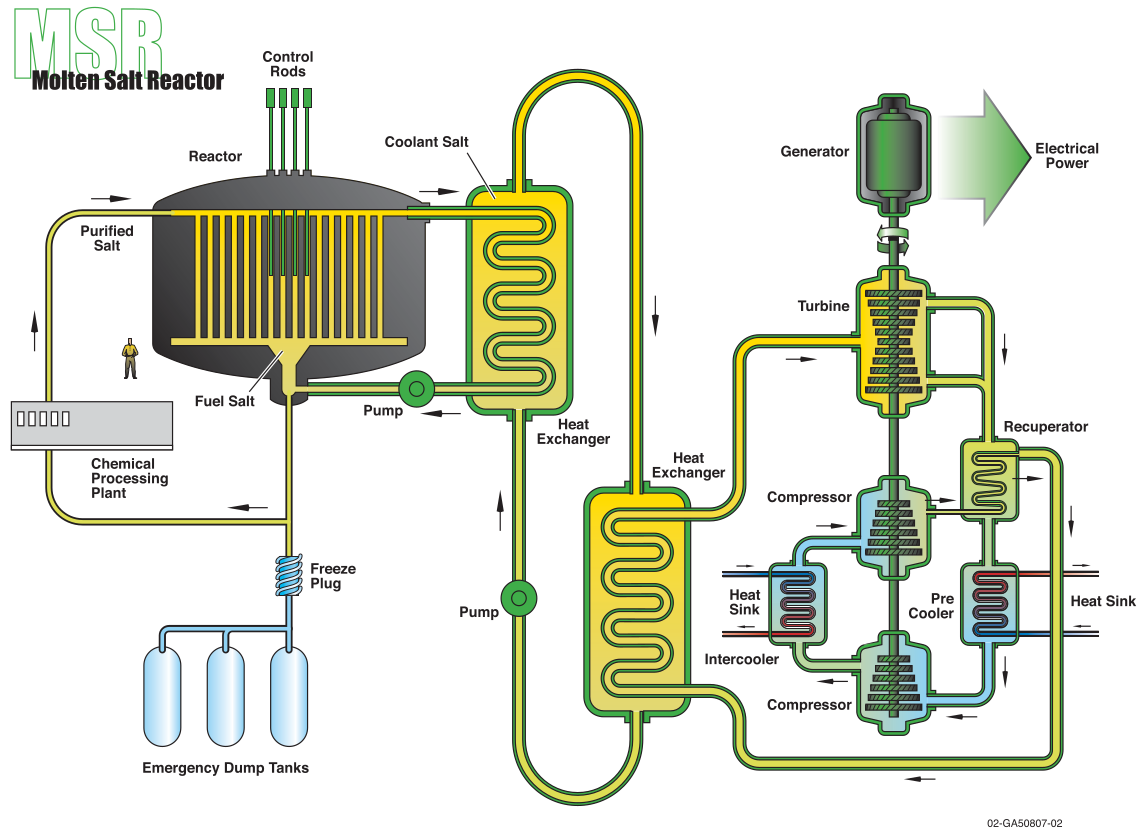
\includegraphics[width=.5\textwidth]{./images/msr}
      \caption{Schematic diagram of a general channel-type MSR concept
      \cite{u.s._doe_nuclear_energy_research_advisory_committee_technology_2002}.}
	  \label{fig:msr}
	\end{figure}
\end{frame}

%\begin{frame}
%  \frametitle{What is a Molten Salt Reactor (MSR)?}
%  \textbf{Advantages of MSRs over other reactor types}
%  \begin{itemize}
%    \item Robust passive safety
%      \begin{itemize}
%        \item strong temperature feedback
%        \item large thermal margin to boiling
%      \end{itemize}
%    \item Freeze plug drains fuel salt into containment tanks under emergency situations
%    \item Online refueling and reprocessing can:
%      \begin{itemize}
%        \item reduce reactor downtime
%        \item reduce required fissile inventory in reactor at any given time
%        \item reduce transuranic waste produced
%        \item allow for $^{233}$U breeding from $^{232}$Th
%      \end{itemize}
%    \item Viable as fast-spectrum breeder/burner reactor
%    \item Can provide high-temperature heat for industrial heat applications
%  \end{itemize}
%\end{frame}

\begin{frame}
  \frametitle{Molten Salt Reactor Modeling \& Simulation}
  \textbf{While modeling MSRs is not necessarily more difficult than modeling solid-fueled
  reactors, we must adapt our software tools to accurately model phenomena unique to MSRs.}\\

  \textbf{Phenomena which pose challenges for MSR modeling}
  \begin{itemize}
	\item Strong multiphysics interactions involving neutron flux, temperature, and flow in the
      reactor core
	  \begin{itemize}
		\item Strong temperature feedback due to thermal expansion of liquid fuel salt
		\item Movement of \gls{DNP} along primary coolant loop
        \item Advection-dominated heat transfer
	  \end{itemize}
    \item Loss of delayed neutrons to out-of-core decay
    \item Complex turbulent flow effects in MSRs
  \end{itemize}
\end{frame}


\subsection{Moltres}
\section{Description of Moltres} \label{sec:moltres-description}

This chapter provides an overview of Moltres as a multiphysics
simulation software for molten salt reactors. 
Section \ref{sec:moltres-features}
describes the general software features of Moltres, Section
\ref{sec:moltres-physics} expands on the physics models in Moltres, and Section
\ref{sec:moltres-previous} describes previous work on \gls{MSR} analysis with Moltres to illustrate
its current capabilities and limitations.

\subsection{General Features} \label{sec:moltres-features}

This section discusses the general software features of Moltres. The
discussion focuses on robustness, extensibility, and ease of use
since these characteristics represent the hallmarks of good multiphysics
software \cite{keyes_multiphysics_2013}. These criteria also apply to
assessing \gls{MSR} simulation tools since the nonlinearity of \gls{MSR}
multiphysics analysis and the complexity of advanced reactor designs
necessitate robust, scalable, and flexible computational tools.

Moltres draws many advantages from being developed on MOOSE
\cite{giudicelli_30_2024}. MOOSE is an open-source, finite-element,
multiphysics framework developed at \gls{INL}. The framework provides a
user-friendly interface for developing multiphysics software through
\gls{OOP} in \texttt{C++} to modularize various
functions relevant to finite-element multiphysics solvers. In this approach,
MOOSE and MOOSE-based applications break down \glspl{PDE} into individual terms
and store them as individual \texttt{C++ objects} referred to as
\texttt{Kernels}. These \texttt{Kernels} contain functions for calculating
their weak form residual and Jacobian
contributions and other relevant functions required to solve a given
\gls{PDE}. \gls{OOP} in MOOSE simplifies software development
since developers can write new \texttt{Kernels} as child classes in
\texttt{C++} derived from existing \texttt{Kernels} (base classes), which share
similar physics to inherit common functions.
The same philosophy applies to all other systems in MOOSE, such as
the \texttt{BCs}, \texttt{Materials}, and \texttt{Postprocessor}
systems for handling relevant boundary conditions, material properties, and
postprocessing calculations, respectively. Overall, this approach also saves
researchers time and effort since they are unencumbered by the technical details
and complexities of programming efficient computational tools for
numerical analysis.

\begin{figure}[htb!]
	\centering
	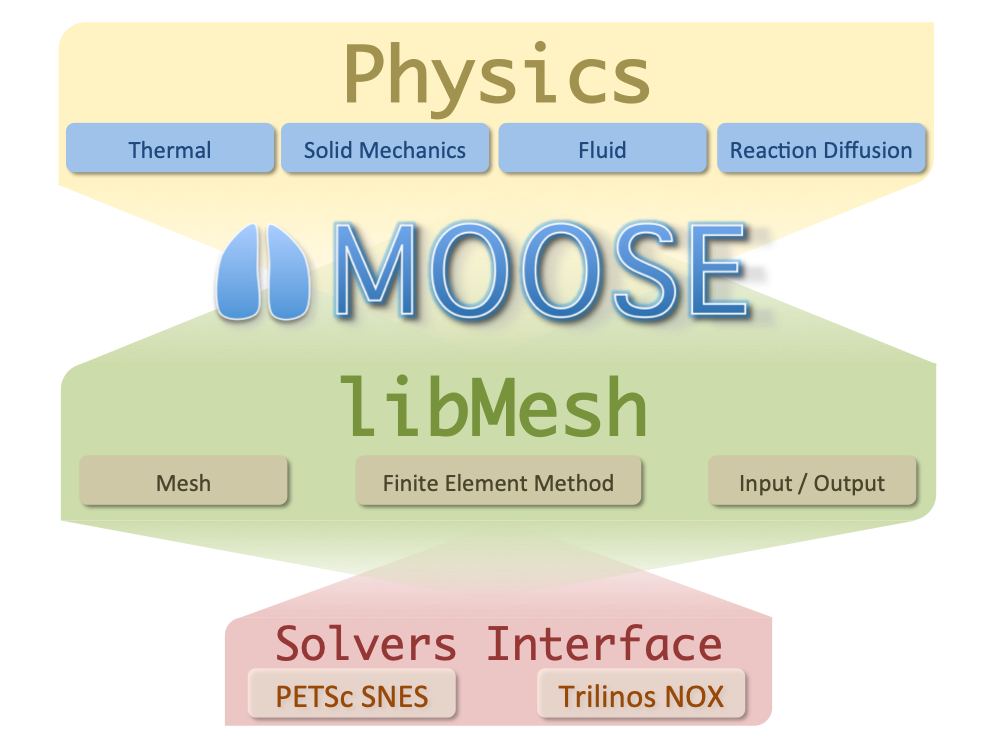
\includegraphics[width=.7\columnwidth]{moose}
	\caption{Structure of MOOSE and its dependencies.}
	\label{fig:moose}
\end{figure}

MOOSE relies on two other open-source libraries: libMesh
\cite{kirk_libmesh_2006} for its \gls{FEM} capabilities on unstructured mesh
and PETSc \cite{satish_petsc_2019} for its nonlinear solvers and
preconditioning routines. By extension, Moltres gains access to these
sophisticated numerical analysis tools and benefits from their continuous
development. Figure
\ref{fig:moose} shows how MOOSE serves as an interface between physics
applications and libMesh/PETSc. MOOSE supports
modeling on up to three-dimensional (3-D) unstructured meshes for a wide range
of mesh file formats, including the commonly used Exodus II file format. For
2-D meshes, users can opt between Cartesian and polar RZ coordinates. MOOSE
also supports parallel computing through the \gls{MPI} library to leverage
modern high-performance computing for large multiphysics simulations.

Moltres benefits from the highly-integrated cross compatibility within the
ecosystem of MOOSE-based applications. MOOSE facilitates multiphysics coupling
among all MOOSE-based applications by providing a common framework for shared
data access and file input/output, thus eliminating computational costs from
data transfers and allowing for fully coupled simulations. For example, Moltres
can couple with the \texttt{Navier-Stokes} module \cite{peterson_overview_2018}
from MOOSE for fully coupled reactor simulations modeling neutronics and
thermal-hydraulics with incompressible flow modeling. Section
\ref{sec:msr-multiphysics} highlighted the advantages of fully coupled schemes
for modeling strongly coupled systems, such as the coupled
neutronics and thermal-hydraulics in \glspl{MSR}. Moltres can also easily
couple to other MOOSE-based applications in a similar fashion. In
addition, MOOSE
provides the option for either tight or loose coupling through the
\texttt{MultiApp} system \cite{gaston_physics-based_2015}. Tight coupling
schemes can outperform fully coupled schemes in weakly coupled systems in which
the computational expenses of fully coupled schemes outweigh the savings from
running fewer Newton iterations due to the superior convergence rate. Loose
coupling schemes help accelerate time-dependent simulations of
stable systems towards a steady state if only the steady-state
configuration interests the user. This situation may occur in the later
stages of \gls{MSR} simulations when the \gls{DNP}
concentrations converge slowly due to their relatively large decay half-lives.
Furthermore, segregated solvers through the \texttt{MultiApp} system enable
Moltres to introduce \gls{DNP} drift and non-uniform
temperature distributions into criticality search simulations. Regardless of
which coupling scheme works best, MOOSE-based applications provide the flexibility
to switch among the schemes as users see fit. For time-dependent simulations,
MOOSE provides more than ten implicit and explicit timestepping
schemes. The default scheme is the first-order backward Euler
method which offers excellent solver stability for stiff \glspl{PDE}.

Lastly, Moltres is an open-source \gls{LGPL} software hosted on
GitHub \cite{github_build_2017}. Open-sourcing software provides ease of access
and expands the user base. These characteristics promote software quality
through increased feedback on users' needs and transparency for peer review.
Open-source software accelerate research progress by supporting
collaboration and sharing best software practices. Supporting Moltres'
continued development, Moltres relies on GitHub for online version control with
continuous integration testing to protect its existing capabilities.

In summary, Moltres provides robust and flexible coupling capabilities to
model strongly coupled neutronics and thermal-hydraulics in \glspl{MSR}. As a
MOOSE-based application, Moltres is highly extensible through coupling with
other MOOSE-based applications and benefits from MOOSE's user-friendly
interface for software development and general ease of use.

\subsection{Physics Models} \label{sec:moltres-physics}

This section describes the various physics models available in Moltres to model
coupled neutronics and thermal-hydraulics in \glspl{MSR}. Section \ref{sec:nts}
discusses the neutronics model in Moltres, Section \ref{sec:th} discusses
the thermal-hydraulics model, and Section \ref{sec:moltres-loop} discusses the
external loop model for \gls{DNP} looping and heat removal via external heat
exchangers.

\subsubsection{Multigroup Neutron Diffusion Model} \label{sec:nts}

Moltres solves the multigroup neutron diffusion equations for the neutron
flux solution within the problem domain. These equations are derived from the
neutron transport equation in the diffusion-dominated limit with Fick's law of
diffusion. They are further simplified by discretizing the continuous neutron energy
variable into a finite number of energy groups \cite{bell_nuclear_1970,
duderstadt_nuclear_1976}. The time-dependent multigroup neutron
diffusion equations with $G$ energy groups and $I$ \gls{DNP}
groups are given by:
%
\begin{align}
    \frac{1}{v_g} \frac{\partial \phi_g}{\partial t} =& \nabla \cdot D_g
    \nabla \phi_g - \Sigma^r_g \phi_g +
    \sum^G_{g' \neq g} \Sigma^s_{g' \rightarrow g} \phi_{g'} \nonumber \\
    &+ \chi^p_g \sum^G_{g'=1} \left( 1-\beta \right) \nu \Sigma^f_{g'}
    \phi_{g'} + \chi^d_g \sum^I_i \lambda_i C_i \label{eq:neutron} %\\
    %
    \shortintertext{where}
    v_g =& \text{ average speed of neutrons in group $g$,} 
    \nonumber \\
    \phi_g =& \text{ neutron flux in group $g$,}
    \nonumber \\
    t =& \text{ time,} \nonumber \\
    D_g =& \text{ diffusion coefficient of neutrons in group $g$,} \nonumber \\
    \Sigma^r_g =& \text{ macroscopic removal cross section for} \nonumber \\
    &\text{ neutrons from group $g$,} \nonumber \\
    \Sigma^s_{g' \rightarrow g} =& \text{ macroscopic scattering cross section
    for neutrons from} \nonumber \\
    &\text{ groups $g'$ to $g$,} \nonumber \\
    \chi^p_g =& \text{ prompt fission spectrum for neutrons in group $g$,} \nonumber \\
    G =& \text{ total number of discrete neutron groups,} \nonumber \\
    \nu_g =& \text{ average number of neutrons produced per fission,} \nonumber
    \\
    \Sigma^f_{g} =& \text{ macroscopic fission cross section for neutron}
    \nonumber \\
    &\text{ in group $g$,} \nonumber \\
    \chi^d_g =& \text{ delayed fission spectrum for neutrons in group $g$,} \nonumber \\
    I =& \text{ total number of \gls{DNP} groups,} \nonumber \\
    \beta =& \text{ total delayed neutron fraction.} \nonumber
\end{align}

Despite forming only around 0.7\% of all neutrons emitted, delayed neutrons
play outsized roles in reactor kinetics. The relatively long half-lives of
\glspl{DNP} give reactor operators ample time in adequately designed reactors
to control reactor power output and intervene in case of power excursions.
The precursor concentration balance equations for $I$ precursor
groups are given by:
%
\begin{align}
    \frac{\partial C_i}{\partial t} =& \beta_i \sum^G_{g'=1} \nu \Sigma^f_{g'}
    \phi_{g'} - \lambda_i C_i - \vec{u} \cdot \nabla C_i + \nabla \cdot
    D_{\text{P}} \nabla C_i \label{eq:precursor} %\\
    %
    \shortintertext{where}
    \beta_i =& \text{ delayed neutron fraction of precursor group $i$,}
    \nonumber \\
    \lambda_i =& \text{ average decay constant of delayed neutron} \nonumber \\
    &\text{ precursors in precursor group $i$,} \nonumber \\
    C_i =& \text{ concentration of \gls{DNP}s in}
    \nonumber \\
    &\text{ precursor group $i$,} \nonumber \\
    \vec{u} =& \text{ molten salt flow velocity vector,}
    \nonumber \\
    D_{\text{P}} =& \text{ effective diffusion coefficient of the delayed}
    \nonumber \\
    &\text{ neutron precursors.} \nonumber
\end{align}

These two equations are largely similar to conventional formulations of the
multigroup neutron diffusion equations with delayed neutrons for most reactor
types. The only differences are in the last two terms in Equation
\ref{eq:precursor}
which represent the advection and diffusion terms, respectively, to model the
movement of \glspl{DNP} in liquid-fuel \glspl{MSR}.

As shown in Equations \ref{eq:neutron} and \ref{eq:precursor}, Moltres requires
group constant data from dedicated high-fidelity neutronics software such as
the NEWT module in SCALE \cite{dehart_reactor_2011}, Serpent
\cite{leppanen_serpent_2014}, or OpenMC \cite{romano_openmc:_2015}. These group
constant data are the neutron energy group $g$ values for $v_g$, $D_g$,
$\Sigma^r_g$, $\Sigma^s_{g' \rightarrow g}$, $\chi^p_g$, $\chi^d_g$,
$\Sigma^f_{g}$, and $\nu\Sigma^f_{g}$, and precursor group $i$ values for
$\beta_i$ and $\lambda_i$. Users
can run a Python script in Moltres' Github repository, which automatically reads
user-provided SCALE/Serpent/OpenMC output data files and creates
Moltres-compatible JSON format files containing all required group constant
data. Moltres allows for an arbitrary number of neutron energy groups $G$ and
precursor groups $I$ as long as the user provides the necessary group constant
data. In practice, $I$ depends on the nuclear data library used to generate
group constants---the JEFF \cite{plompen_joint_2020} and ENDF
\cite{brown_endfb-viii0_2018} data libraries define eight precursor groups
and six precursor groups, respectively.

In multiphysics reactor simulations, we model the coupling between neutronics
and thermodynamics through temperature-dependent group constants. To sample
group constants at different temperatures in Moltres, users must provide group
constant data measured at more than one temperature (e.g., 800K--1500K at 100K
intervals). Users can then choose from linear spline, cubic spline, or monotone
cubic interpolation methods available in Moltres to interpolate the group
constant data for values falling within the provided temperature range. 

Moltres provides two types of boundary conditions for neutron fluxes; these are
conventionally known as the vacuum and reflective boundary conditions given,
respectively, as:

\begin{align}
  D_g \nabla \phi_g \cdot \hat{n} + \frac{\phi}{2} =& 0 \label{eq:vacuum}
    \shortintertext{and}
  \nabla \phi \cdot \hat{n} =& 0
    \shortintertext{where}
  \hat{n} =& \mbox{ outward unit normal vector to the boundary.} \nonumber
\end{align}

The vacuum boundary condition typically applies to the external boundaries of
the reactor beyond which lies low-interaction media such as air. The
reflective boundary condition is useful for exploiting symmetries in the
model geometry, such as along the axial boundary in axisymmetric geometries. The
reflective boundary condition is equivalent to the more generally known
homogeneous Neumann boundary condition. Relevant boundary conditions for
\glspl{DNP} include the homogeneous Neumann boundary condition
along fuel salt-structural interfaces and outflow/inflow boundary
conditions along the outlet/inlet boundaries through which the precursors
flow as they circulate the fuel salt loop.

\subsubsection{Incompressible Flow Model} \label{sec:th}

Moltres relies on MOOSE's \texttt{Heat} \texttt{Conduction} and
\texttt{Navier-Stokes} physics modules for its thermal-hydraulics modeling
capabilities. While the \texttt{Navier-Stokes} module supports
compressible and incompressible flow modeling, this work focuses on
multiphysics coupling in \glspl{MSR} with the latter. The
time-dependent incompressible Navier-Stokes equations for velocity $\vec{u}$
with the Boussinesq approximation for buoyancy-driven flow are given as:

\begin{align}
    \text{Momentum equation: } \rho \frac{\partial \vec{u}}{\partial t} =&
    -\rho (\vec{u}
    \cdot \nabla) \vec{u} - \nabla p + \mu \nabla^2 \vec{u}
    + \rho \alpha \vec{g} \left(T - T_{\text{ref}} \right)
    \label{eq:momemtum}
    \shortintertext{and}
    \text{Mass equation: } \nabla \cdot \vec{u} =& 0
    \label{eq:divergence}
    \shortintertext{where}
    \rho =& \text{ fluid density,} \nonumber \\
    p =& \text{ pressure,} \nonumber \\
    \mu =& \text{ dynamic viscosity,} \nonumber \\
    \alpha =& \text{ coefficient of thermal expansion,} \nonumber \\
    \vec{g} =& \text{ gravitational force vector,} \nonumber
    \\
    T =& \text{ fluid temperature,} \nonumber \\
    T_{\text{ref}} =& \text{ reference temperature at which the nominal}
    \nonumber \\
    &\text{ density is provided.} \nonumber
    \nonumber
\end{align}

Velocity variables and advected quantities such as temperature are susceptible
to numerical node-to-node oscillations
commonly observed when resolving advection-dominated flows using continuous
Galerkin methods \cite{kuhlmann_lid-driven_2018}. The \texttt{Navier-Stokes}
module provides the \gls{SUPG} stabilization scheme
\cite{brooks_streamline_1982} for the velocity and temperature variables to
minimize these oscillations. The module also provides the \gls{PSPG}
stabilization scheme \cite{hughes_new_1986}, enabling equal-order
discretizations of pressure and velocity. Peterson et al. \cite{peterson_overview_2018}
provide further detail on the implementation of these stabilization schemes in
the \texttt{Navier-Stokes} module.

\subsubsection{Temperature Advection-Diffusion Model}

Lastly, Moltres solves for the temperature distribution through the temperature
advection-diffusion equation given by:

\begin{align}
    \rho c_{p} \frac{\partial T}{\partial t} =& - \rho c_p \vec{u}
    \cdot \nabla T + \nabla \cdot \left(k \nabla T \right) + Q_f - Q_s
    \label{eq:temp}
    \shortintertext{and}
    Q_f =& \sum^G_{g=1} \epsilon_g \Sigma_g^f \phi_g \label{eq:heat-source}
    \shortintertext{where}
    c_p =& \text{ specific heat capacity of molten salt,} \nonumber \\
    k =& \text{ effective thermal conductivity of molten salt,} \nonumber \\
    Q_f =& \text{ fission heat source,} \nonumber \\
    \epsilon_g =& \text{ average fission energy released by neutrons in group
    $g$,} \nonumber \\
    Q_s =& \text{ heat sink/removal.} \nonumber
\end{align}

$Q_f$ represents the fission heat source term and is calculated by taking the
sum of neutron group fluxes multiplied by their respective macroscopic fission
cross sections and the average fission energy released per fission.

The \texttt{Navier-Stokes} module provides the following types of boundary
conditions for the velocity and temperature variables:

\begin{align}
    \text{Dirichlet: }& & u \ \left(\text{or } T\right) =& c & \\
    \text{Homogeneous Neumann: }& & \frac{\partial u}{\partial x_i} \
    \left(\text{or } \frac{\partial T}{\partial x_i}\right) =& 0 & \\
    \text{``No boundary condition'' outflow: }& &
    \left[ \nabla \vec{u} + \left(\nabla \vec{u} \right)^T \right] \cdot
    \hat{n} =& 0 \ \text{ (velocity)} & \\
    \text{``No boundary condition'' outflow: }& &
    k \nabla T \cdot\hat{n} =& 0 \ \text{ (temperature)} &
    \shortintertext{where}
    & & c =& \text{ user-defined constant value,} & \nonumber \\
    & & \hat{n} =& \text{ unit normal vector to the boundary.} & \nonumber
\end{align}

The Dirichlet boundary condition can be used to set the inlet velocities and
temperatures and no-slip conditions along solid boundaries. The
homogeneous Neumann boundary condition is commonly
imposed along the outlet boundary. However, the latter approach
artificially influences upstream behavior, especially in developing flow. The
``no boundary condition'' outflow boundary condition by Griffiths
\cite{griffiths_no_1997} has been shown to reduce such upstream errors.

\subsubsection{External Loop Model} \label{sec:moltres-loop}

Moltres also accounts for the decay of
\glspl{DNP} outside the active core region by simulating its flow in a
separate 1-D pipe geometry. This external loop pipe calculation is tightly
coupled to the active core simulation through Picard iterations in MOOSE's
MultiApp \cite{gaston_physics-based_2015} functionality and inlet/outlet boundary values.
The external loop region is assumed to be subcritical to minimize neutron
irradiation upon heat exchangers, pumps, and other equipment. Therefore, the
only significant neutronic-related phenomena are the drift and decay of
\glspl{DNP}. The governing equation for the \glspl{DNP} is:
%
\begin{align}
    \frac{\partial C_i}{\partial t} =& - \lambda_i C_i - u
    \frac{\partial C_i}{\partial x}.
    \label{eq:dnploop}
\end{align}
%
Equation \ref{eq:dnploop} is derived from equation \ref{eq:precursor} by
removing the fission \gls{DNP} source and diffusion terms and reducing the
dimensionality from 3-D to 1-D.

Moltres also simulates the temperature distribution in the external loop to model heat removal via
heat exchangers. The governing equation
for temperature, derived from equation \ref{eq:temp}, is:
%
\begin{align}
    \rho c_{p} \frac{\partial T}{\partial t} =& - \rho c_p u
    \frac{\partial T}{\partial x} - Q_{hx} \label{eq:temploop}
    \shortintertext{where}
    Q_{hx} =& \text{heat removal rate through the heat exchanger.} 
    \nonumber
\end{align}
%
The fission heat source term is replaced with a heat
exchanger sink term $Q_{hx}$.

Table \ref{table:loopbc} lists the boundary conditions for all variables on the inlet and outlet of
the 1-D external loop region. The inlet boundary conditions are all Dirichlet boundary conditions. The
prescribed value for the inlet boundary conditions are set to match the average outflow from the
active core region. The outlet boundary conditions are all outflow boundary conditions, as shown in
Table \ref{table:loopbc}.

\begin{table}[htbp!]
    \small
	\caption{Boundary conditions in the 1-D external loop geometry. $u$
	represents the 1-D velocity in this region.}
	\centering
	\begin{tabular}{ l l c}
		\toprule
		Variable & Boundary & Boundary Condition \\
        \midrule
        \multirow{2}{*}{Delayed neutron precursor concentration $C_i$} &
        Inlet (Core) & $C_i = c$ \\
        & Outlet (Core) & $u \cdot C_i = 0$ \\
        \midrule
        \multirow{2}{*}{Temperature $T$} &
        Inlet (Core) & $T = c$ \\
        & Outlet (Core) & $u \cdot T = 0$ \\
		\bottomrule
	\end{tabular}
	\label{table:loopbc}
\end{table}

\subsubsection{Core and External Loop Coupling Model}

This subsection details the \gls{DNP} and
temperature coupling between the core and external loop regions. 

At every timestep, Moltres calculates weighted averages of the
temperature and the precursors at the outlet. These values are weighted by the
outflow velocity values at the outlet according to the following equation:
%
\begin{align}
    \overline{\psi} =& \frac{\int_\mathcal{C} Y(x_j) u(x_j) dx_j}{
    \int_\mathcal{C} u(x_j) dx_j} \\
    \shortintertext{where}
    Y =& \text{ variable to be weighted} \nonumber \\
    \mathcal{C} =& \text{ outlet boundary area} \nonumber \\
    u =& \text{ outflow velocity perpendicular to the outlet boundary,} \nonumber \\
    x_j =& \text{ spatial coordinate parallel to the outlet boundary.}
    \nonumber
\end{align}

Moltres transfers this outflow value from the core region to the 1-D
external loop region to be used as the boundary value for the inhomogeneous
Dirichlet boundary
condition at the inlet. Likewise, the outflow value from the external
loop region is used for the inflow value in the central core region. No
averaging is required for this step as the external loop region is a 1-D system.
This approach results in uniform inflow temperature and \gls{DNP} at the
inlet. The Picard iterations within every timestep ensure the two systems
are tightly coupled.

\subsection{Previous \gls{MSR} Analyses with Moltres} \label{sec:moltres-previous}

This section discusses some previous work with Moltres to illustrate its
various capabilities and coupling approaches for multiphysics \gls{MSR}
modeling and simulation. Section \ref{sec:msre} summarizes the work by Lindsay et
al. \cite{lindsay_introduction_2018} in modeling the \gls{MSRE}, and Section
\cite{park_advancement_2020} summarizes my previous work in modeling the
\gls{MSFR}.

\subsubsection{Introduction to Moltres and Modeling the MSRE} \label{sec:msre}

This section follows the work by Lindsay et al. in \textit{Introduction to Moltres:
An Application for Simulation of Molten Salt Reactors}
\cite{lindsay_introduction_2018}.

In 2017, Lindsay et al. introduced
Moltres to the \gls{MSR} community for multiphysics simulations of \glspl{MSR}.
Their work showcased neutron diffusion and thermal-hydraulics coupling
capabilities in Moltres. The authors
demonstrated these capabilities by running time-dependent simulations of 2-D
axisymmetric and 3-D \gls{MSRE} models until the flux, precursor, and
temperature distributions reached a steady state.

\begin{figure}[htb!]
	\centering
	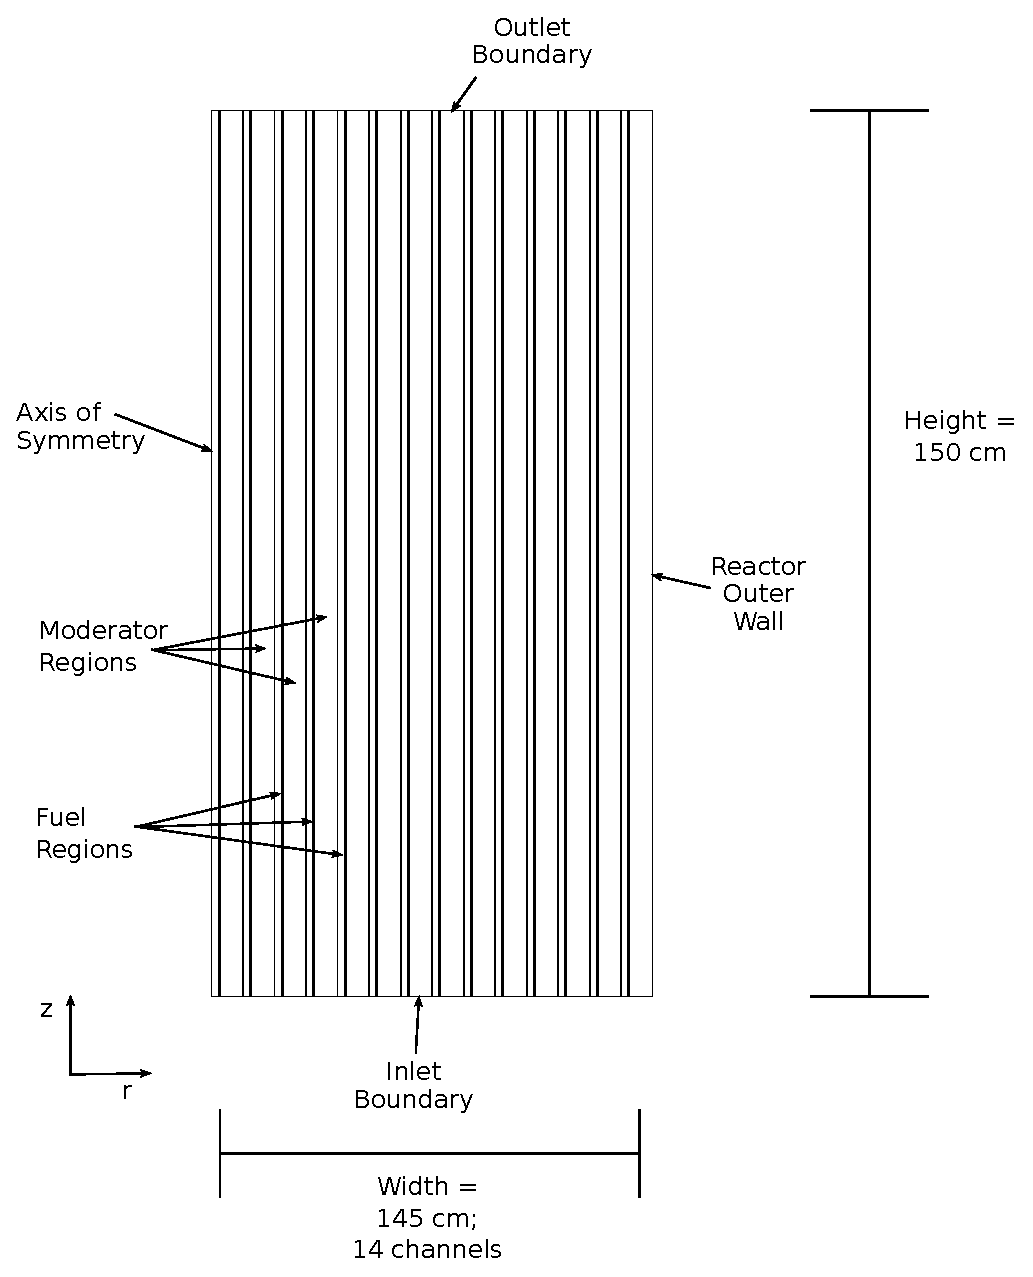
\includegraphics[width=.45\columnwidth]{msre-geometry}
	\caption{Schematic diagram of the 2-D axisymmetric \gls{MSRE} geometry
	adopted by Lindsay et al. \cite{lindsay_introduction_2018}.}
	\label{fig:msre-geometry}
\end{figure}

Figure \ref{fig:msre-geometry} shows the fuel channels and moderator regions of
the 2-D \gls{MSRE} geometry that Lindsay et al. adopted for their study.
They ran a two-group neutron diffusion model with six precursor groups and
vacuum boundary conditions on the outer boundaries governed by Equations
\ref{eq:neutron}, \ref{eq:precursor}, and \ref{eq:vacuum} shown in Section
\ref{sec:nts}. They modeled precursor drift due to fuel salt flow by imposing
fixed uniform flow upwards through the fuel channels shown in Figure
\ref{fig:msre-geometry}. Their thermal-hydraulics model employed a
governing equation for temperature in the fuel salt equivalent to Equation
\ref{eq:temp} with fixed uniform flows while imposing a cosine-shaped heat
source term representing heat dissipation from gamma and neutron irradiation in
the graphite moderator region. In addition, all governing equations were fully
coupled and solved simultaneously as a single system of equations with implicit
Euler timestepping to accurately and efficiently resolve the strong coupling
expected between the neutronics and temperature.

\begin{figure}[htb!]
	\centering
	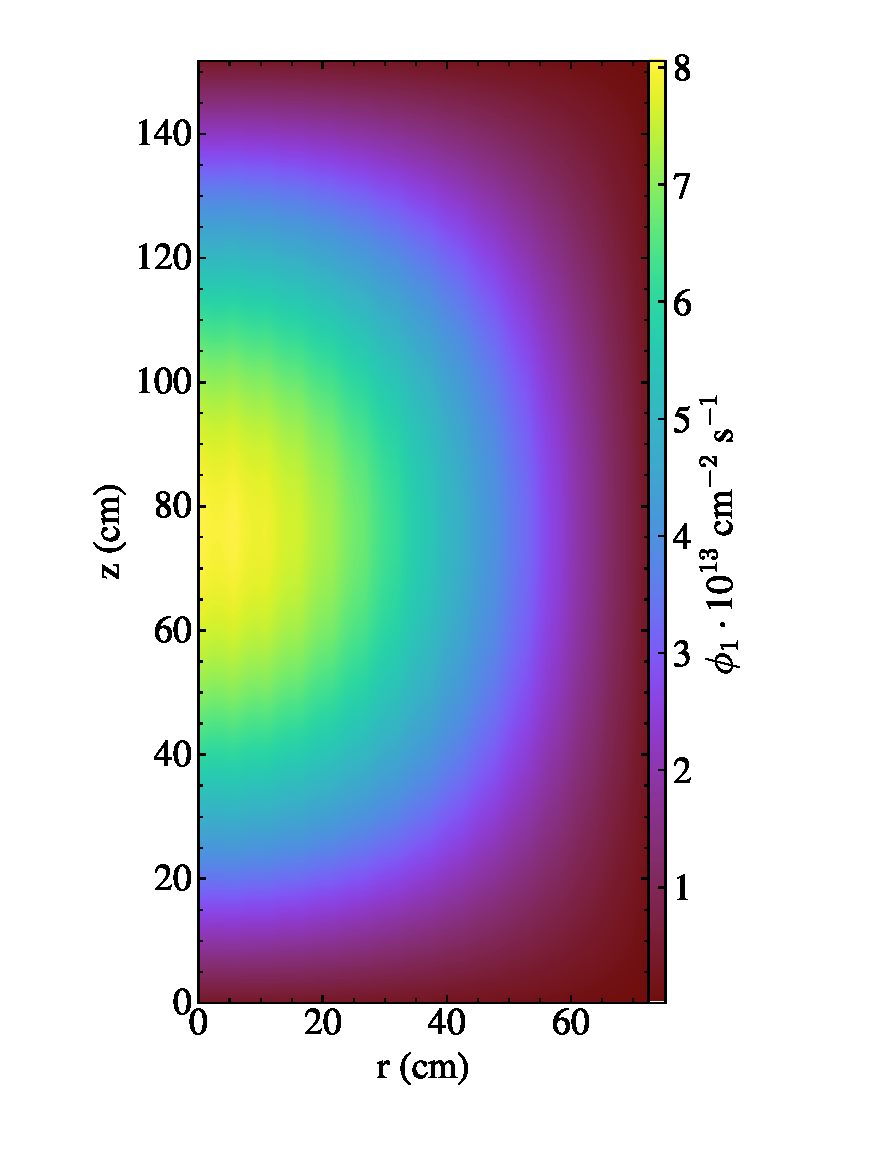
\includegraphics[width=.45\columnwidth]{2d_gamma_heating_group1}
	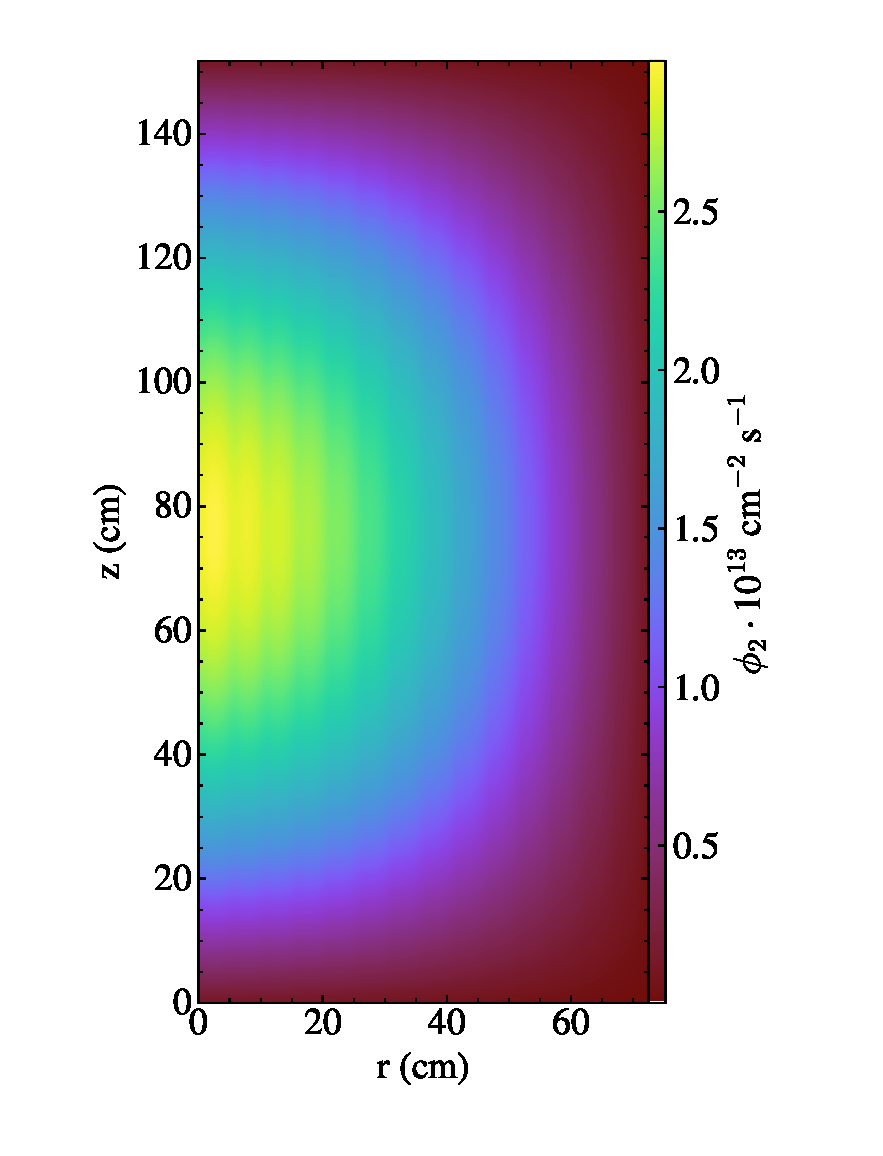
\includegraphics[width=.45\columnwidth]{2d_gamma_heating_group2}
	\caption{Neutron group 1 and 2 fluxes in the 2-D axisymmetric \gls{MSRE}
	model from Lindsay et al. \cite{lindsay_introduction_2018}.}
	\label{fig:msre-flux}
\end{figure}

\begin{figure}[htb!]
	\centering
	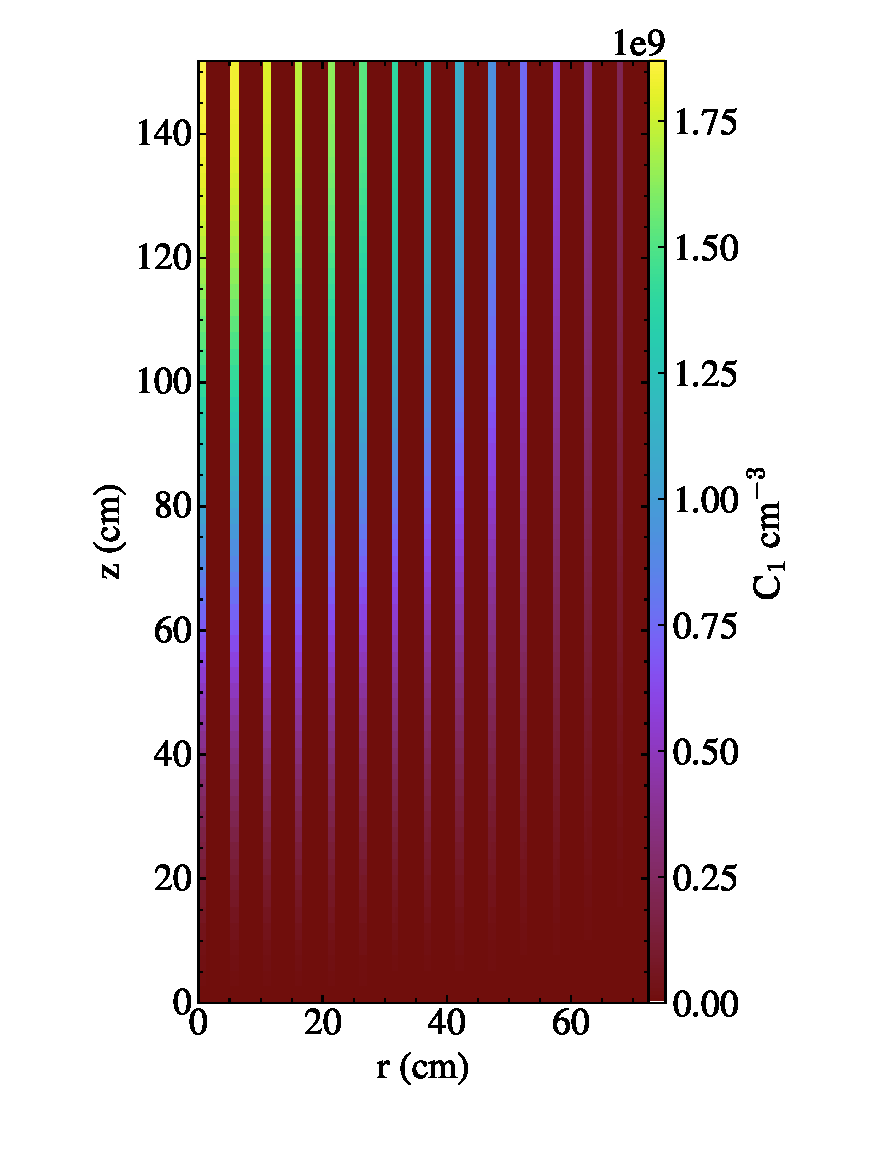
\includegraphics[width=.45\columnwidth]{2d_gamma_heating_pre1_scaled}
	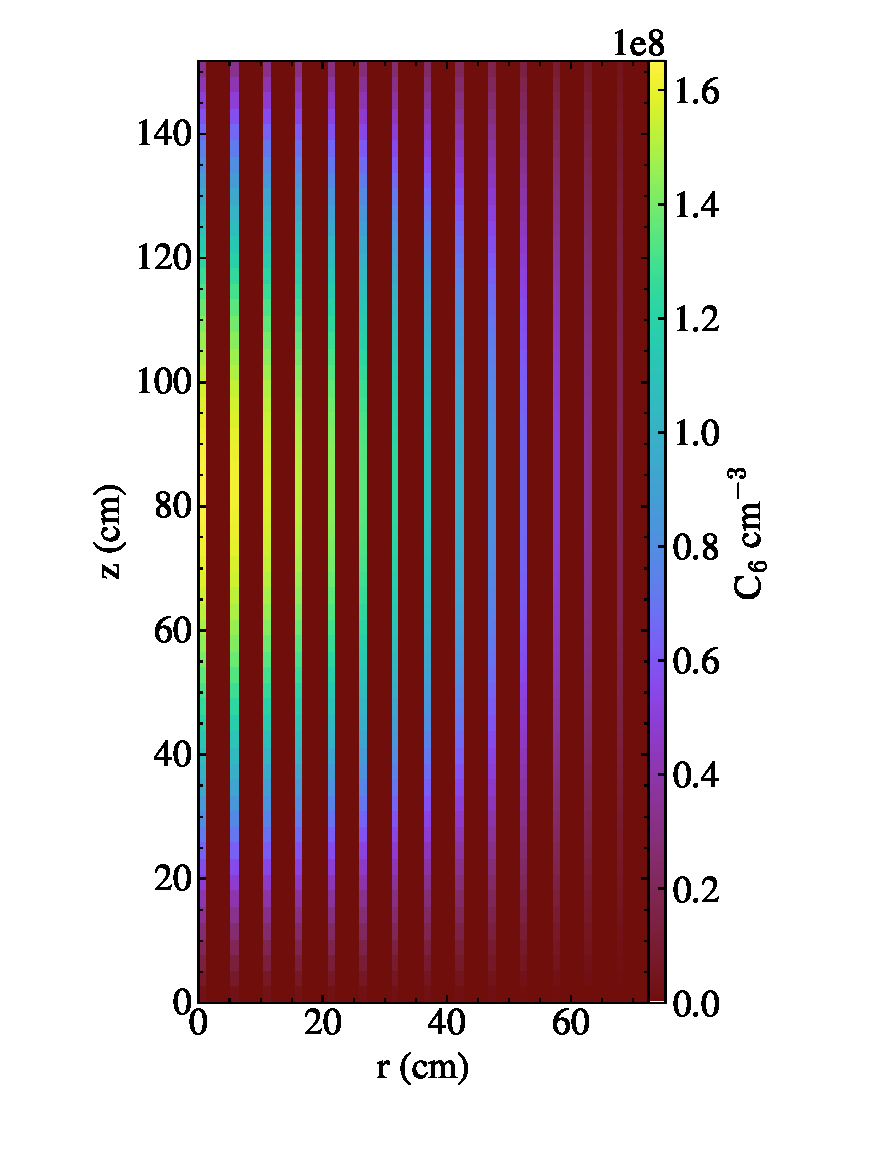
\includegraphics[width=.45\columnwidth]{2d_gamma_heating_pre6_scaled}
	\caption{Longest- and shortest-lived precursor concentrations ($\lambda =
	1.24\times 10^{-2}$s$^{-1}$ and $3.07$s${-1}$, respectively) in the 2-D
	axisymmetric \gls{MSRE} model from Lindsay et al.
	\cite{lindsay_introduction_2018}.}
	\label{fig:msre-precursor}
\end{figure}

\begin{figure}[htb!]
	\centering
	\begin{minipage}[b]{0.45\columnwidth}
	    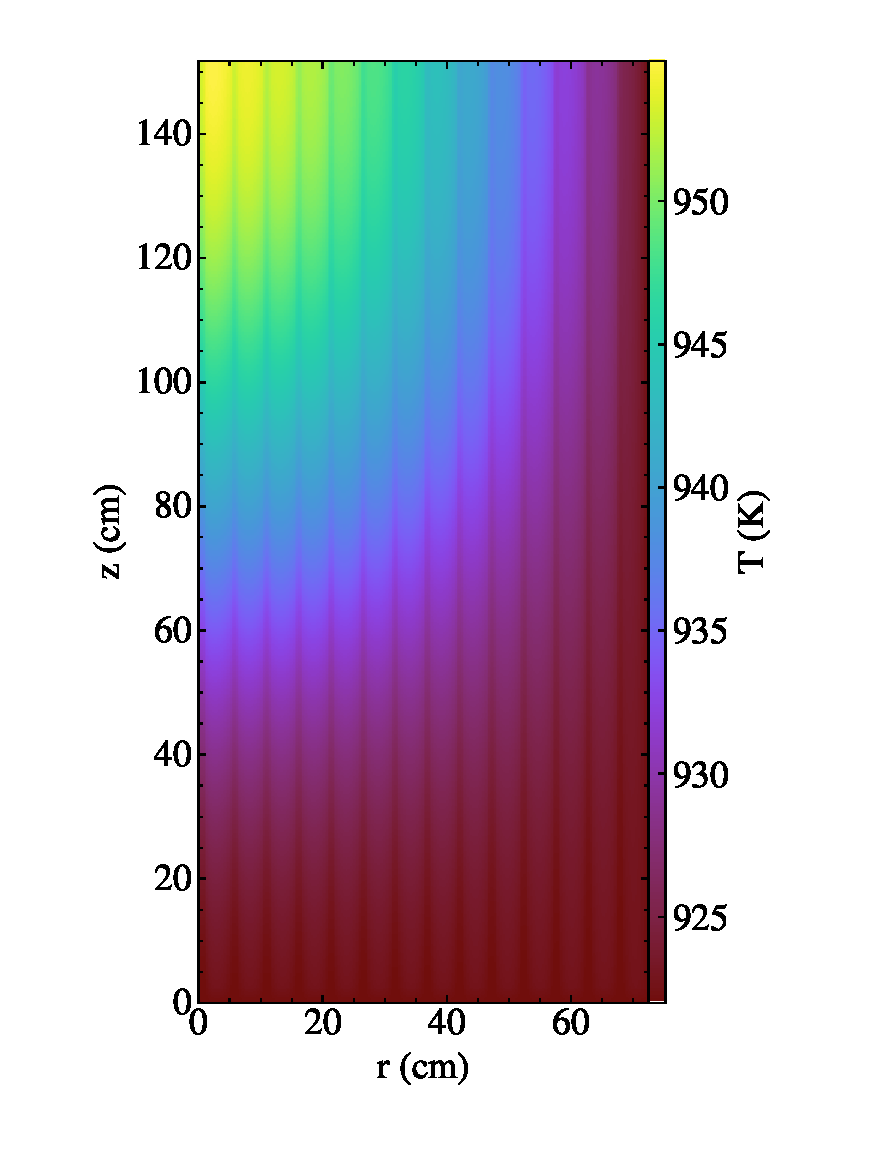
\includegraphics[width=\columnwidth]{2d_gamma_heating_temp}
	    \caption{Temperature distribution in the 2-D
	    axisymmetric \gls{MSRE} model from Lindsay et al.
	    \cite{lindsay_introduction_2018}.}
	    \label{fig:msre-temp}
	\end{minipage}
	\hfill
	\begin{minipage}[b]{0.45\columnwidth}
	    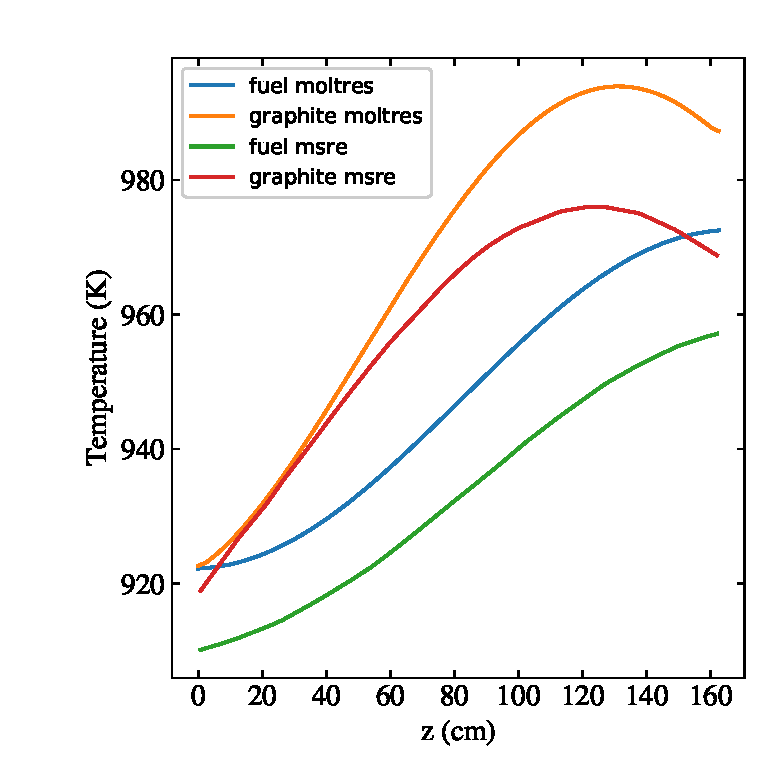
\includegraphics[width=\columnwidth]{combined_msre_moltres_axial_temps}
	    \caption{Moltres \cite{lindsay_introduction_2018} and \gls{ORNL}
	    \gls{MSRE} \cite{briggs_molten-salt_1964} axial temperature
	    distributions in the hottest fuel channel and adjacent graphite.}
	    \label{fig:msre-temp-plot}
	\end{minipage}
\end{figure}

Figure \ref{fig:msre-flux} shows the fast and thermal neutron fluxes
corresponding to group 1 and 2 in the 2-D \gls{MSRE} model. As expected, the
fluxes exhibit general cosine shapes in the axial and radial directions. We
also observe minor oscillations in the radial direction coinciding with the
regular fuel and moderator lattice. The fuel regions favor the fast flux, while
the moderator regions favor the thermal flux.

Figure \ref{fig:msre-precursor}
shows the longest- and shortest-lived precursor concentrations in the fuel
channels. With a long half-life of 55.9 s relative to the 6.91 s it takes for
salt to flow from bottom to top, the longest-lived precursor concentration peaks
outside the model domain. By contrast, the shortest-lived precursor
concentration closely follows the neutron fluxes' cosine shape, which
dictate where the precursors are born.

Finally, Figure \ref{fig:msre-temp}
shows the temperature distribution in the 2-D \gls{MSRE} model. The temperature
naturally peaks near the outlet due to upward advection. The moderator regions
experience hotter temperatures than the fuel regions due to radiative heating
and the relative inefficiency of heat conduction in the graphite compared to
advection in the fuel salt.

\begin{figure}[htb!]
	\centering
	\begin{subfigure}[h]{0.45\columnwidth}
	    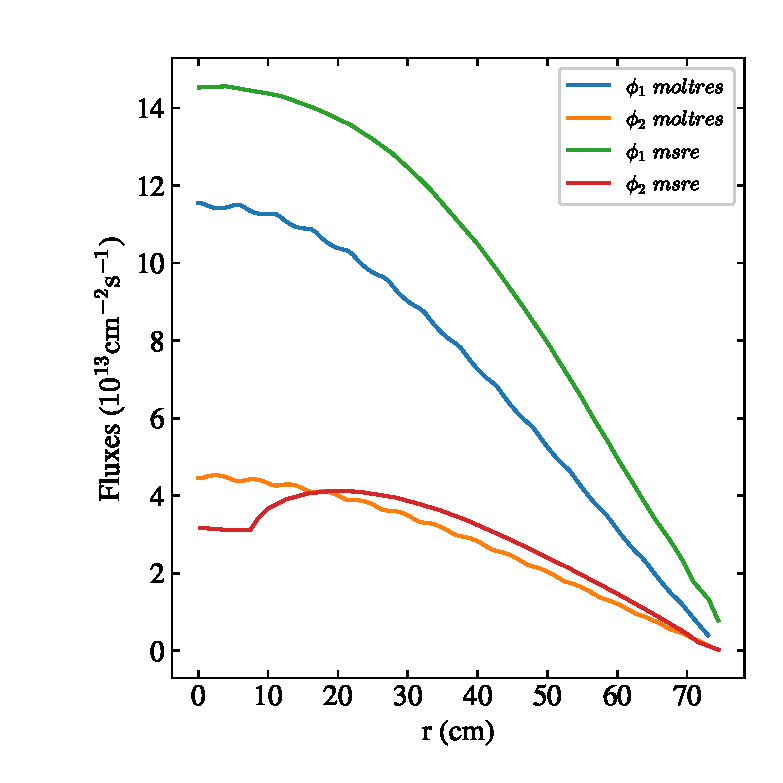
\includegraphics[width=\columnwidth]{combined_msre_moltres_radial}
	    \caption{Radial fluxes at reactor half-height.}
	    \label{fig:msre-flux-radial}
	\end{subfigure}
	\hfill
	\begin{subfigure}[h]{0.45\columnwidth}
	    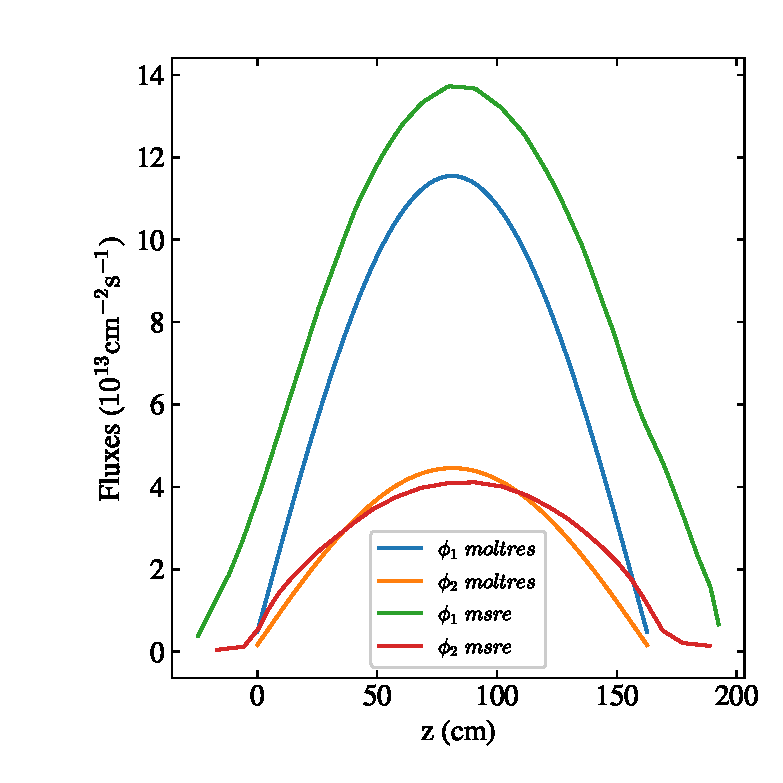
\includegraphics[width=\columnwidth]{combined_msre_moltres_axial}
	    \caption{Axial fluxes along the core centerline ($r=0$ cm).}
	    \label{fig:msre-flux-axial}
	\end{subfigure}
	\caption{The fast and thermal fluxes from
	Moltres \cite{lindsay_introduction_2018} and the \gls{ORNL} \gls{MSRE}
	design calculations \cite{briggs_molten-salt_1964}.}
\end{figure}

The corresponding neutronics and thermal-hydraulics results from their 3-D model
show good qualitative agreement with the 2-D results. Given the lack of
\gls{MSR} experimental data, they compared their 2-D model results with
\gls{MSRE} design calculations performed using legacy software in 1963-1964 at
\gls{ORNL}. Their neutron flux and temperature distribution results showed good
qualitative agreement with \gls{ORNL} data. The authors attributed
discrepancies to the following differences in the two modeling approaches: the
absence of axial heat conduction and the use of 32 neutron groups in the
\gls{ORNL} calculations, and the exclusion of control rod thimbles in the
Moltres calculations.

\paragraph{Critical Assessment} \label{sec:msre-critique}

Lindsay et al.'s work illustrated early development efforts for neutronics and thermal-hydraulics
models in Moltres. It demonstrated, along with advanced capabilities from the \gls{MOOSE}
framework, fully-coupled simulations of the \gls{MSRE} with implicit timestepping. The
decent qualitative agreement observed between Moltres and the \gls{ORNL}
\gls{MSRE} calculations proved that Moltres could simulate
\glspl{MSR} under some simplifying assumptions.

On the other hand, significant improvements could be made to Moltres to better
model multiphysics phenomena in \glspl{MSR}. For instance, replacing the
fixed uniform salt flow with a proper flow profile governed by fluid flow
equations would accurately capture precursor and temperature advection.
Temperature advection has a particularly large impact on the temperature
distribution in the fuel salt since molten salts generally have large Prandtl
numbers, which measure the ratio of convective to conductive heat transfer.
The flow-modeling feature would be of even greater importance when modeling
pool-type \glspl{MSR}, which consist of a single large fuel salt region in the
reactor core.

Another essential feature for modeling \glspl{MSR}, which was already under
development at the time of publication, is a precursor loop
system to recirculate precursors back into the core. While some precursors
decay outside the core, others survive long enough to recirculate back into the
core. The loop system would provide a more accurate estimate of the delayed
neutron fraction instead of discarding all precursors that flowed out of
the core. In transient simulations involving sudden increases in the neutron
flux, precursors recirculating into the core can induce observable jumps and
dips in the power output due to the associated reactivity insertion from the
delayed neutrons.

Moltres would also benefit from a decay heat model which Lindsay
et al. mentioned in their work \cite{lindsay_introduction_2018},
especially for transient accident analyses. While decay heat from fission
product decays represents a small fraction ($\sim5\%$) of total power output,
this heat source can be significant in unprotected loss of flow or loss of
secondary cooling accidents. Therefore, understanding residual heat generation
from fission product decays in \gls{MSR} is essential in preventing further
structural failure after an accident.

Specific to reactor physics modeling, Moltres also requires an accurate method for modeling
control rods. As observed in Figure \ref{fig:msre-flux}, the omission of control rods led to
significant discrepancies in the thermal flux distribution. However, developing control rod
modeling capability in Moltres is nontrivial given that neutron diffusion theory performs poorly
within highly neutron-absorbing regions.

Lastly, the authors recognized two other avenues for future work: further \gls{VV} of Moltres'
capabilities by comparison
with more detailed experimental data and other modern \gls{MSR} modeling
efforts; and the study of transient simulation cases such as control rod
ejection, single channel blockage, loss of flow, and loss of secondary cooling.

\subsubsection{Advancements in Moltres and Transient Simulations of the MSFR}
\label{sec:msfr}

This section follows my previous work for my Master's degree in \textit{Advancement and
Verification of Moltres for Molten Salt Reactor Safety Analysis} \cite{park_advancement_2020},
which I shall refer to as ``this work'' in this subsection.

In many ways, this work represents a continuation of the work by Lindsay et al.
\cite{lindsay_introduction_2018} in developing Moltres as an \gls{MSR}
simulation tool. New features introduced include coupling the existing
neutronics and temperature equations to incompressible Navier-Stokes equations
to model flow dynamics, the precursor loop system, and the decay heat model.
I later demonstrated these features through steady-state and transient
simulations of a 2-D axisymmetric \gls{MSFR} model.

Moltres couples natively with the \texttt{Navier-Stokes} module in \gls{MOOSE} for
incompressible flow modeling capabilities. Section \ref{sec:th} describes the governing equations
for incompressible flow and temperature advection-diffusion.
The precursor loop model was developed to model
precursor recirculation into the core. The precursor loop system leverages
the \texttt{MultiApp} system in \gls{MOOSE} to couple a 1-D pipe model to the
core to simulate precursor flow outside the core. The core and the pipe models
are coupled via inlet and outlet boundary conditions, as detailed in Section
\ref{sec:moltres-loop}. The loop system can also accommodate a pointwise heat
exchanger model with a heat removal rate as a function of time
or auxiliary variables in the Moltres simulation.

In addition, I developed a decay heat model to simulate delayed heat release
from the decay of fission products, similar to delayed neutron emission
from precursors. The decay heat model introduces decay heat groups of different
decay constants and variables representing the decay heat groups and modifies the
heat source term given by Equation \ref{eq:heat-source} to account for
the delayed heat generation. 

The number of decay heat groups depends on
the decay heat profile of the reactor after a specified period of operation.
Determining the decay heat profile requires fuel depletion calculations to
obtain the fuel composition during/after reactor operation and subsequent
calculations for the cumulative decay heat released from individual isotopes.
In this work, I cited results by Aufiero et al. \cite{aufiero_extended_2013},
who determined that three decay heat groups ($J=3$) were sufficient to
reproduce the decay heat profile of the \gls{MSFR} equilibrium fuel composition
for up to 300 seconds after shutdown with a relative error of less than 2\%.

\begin{figure}[htb!]
	\centering
	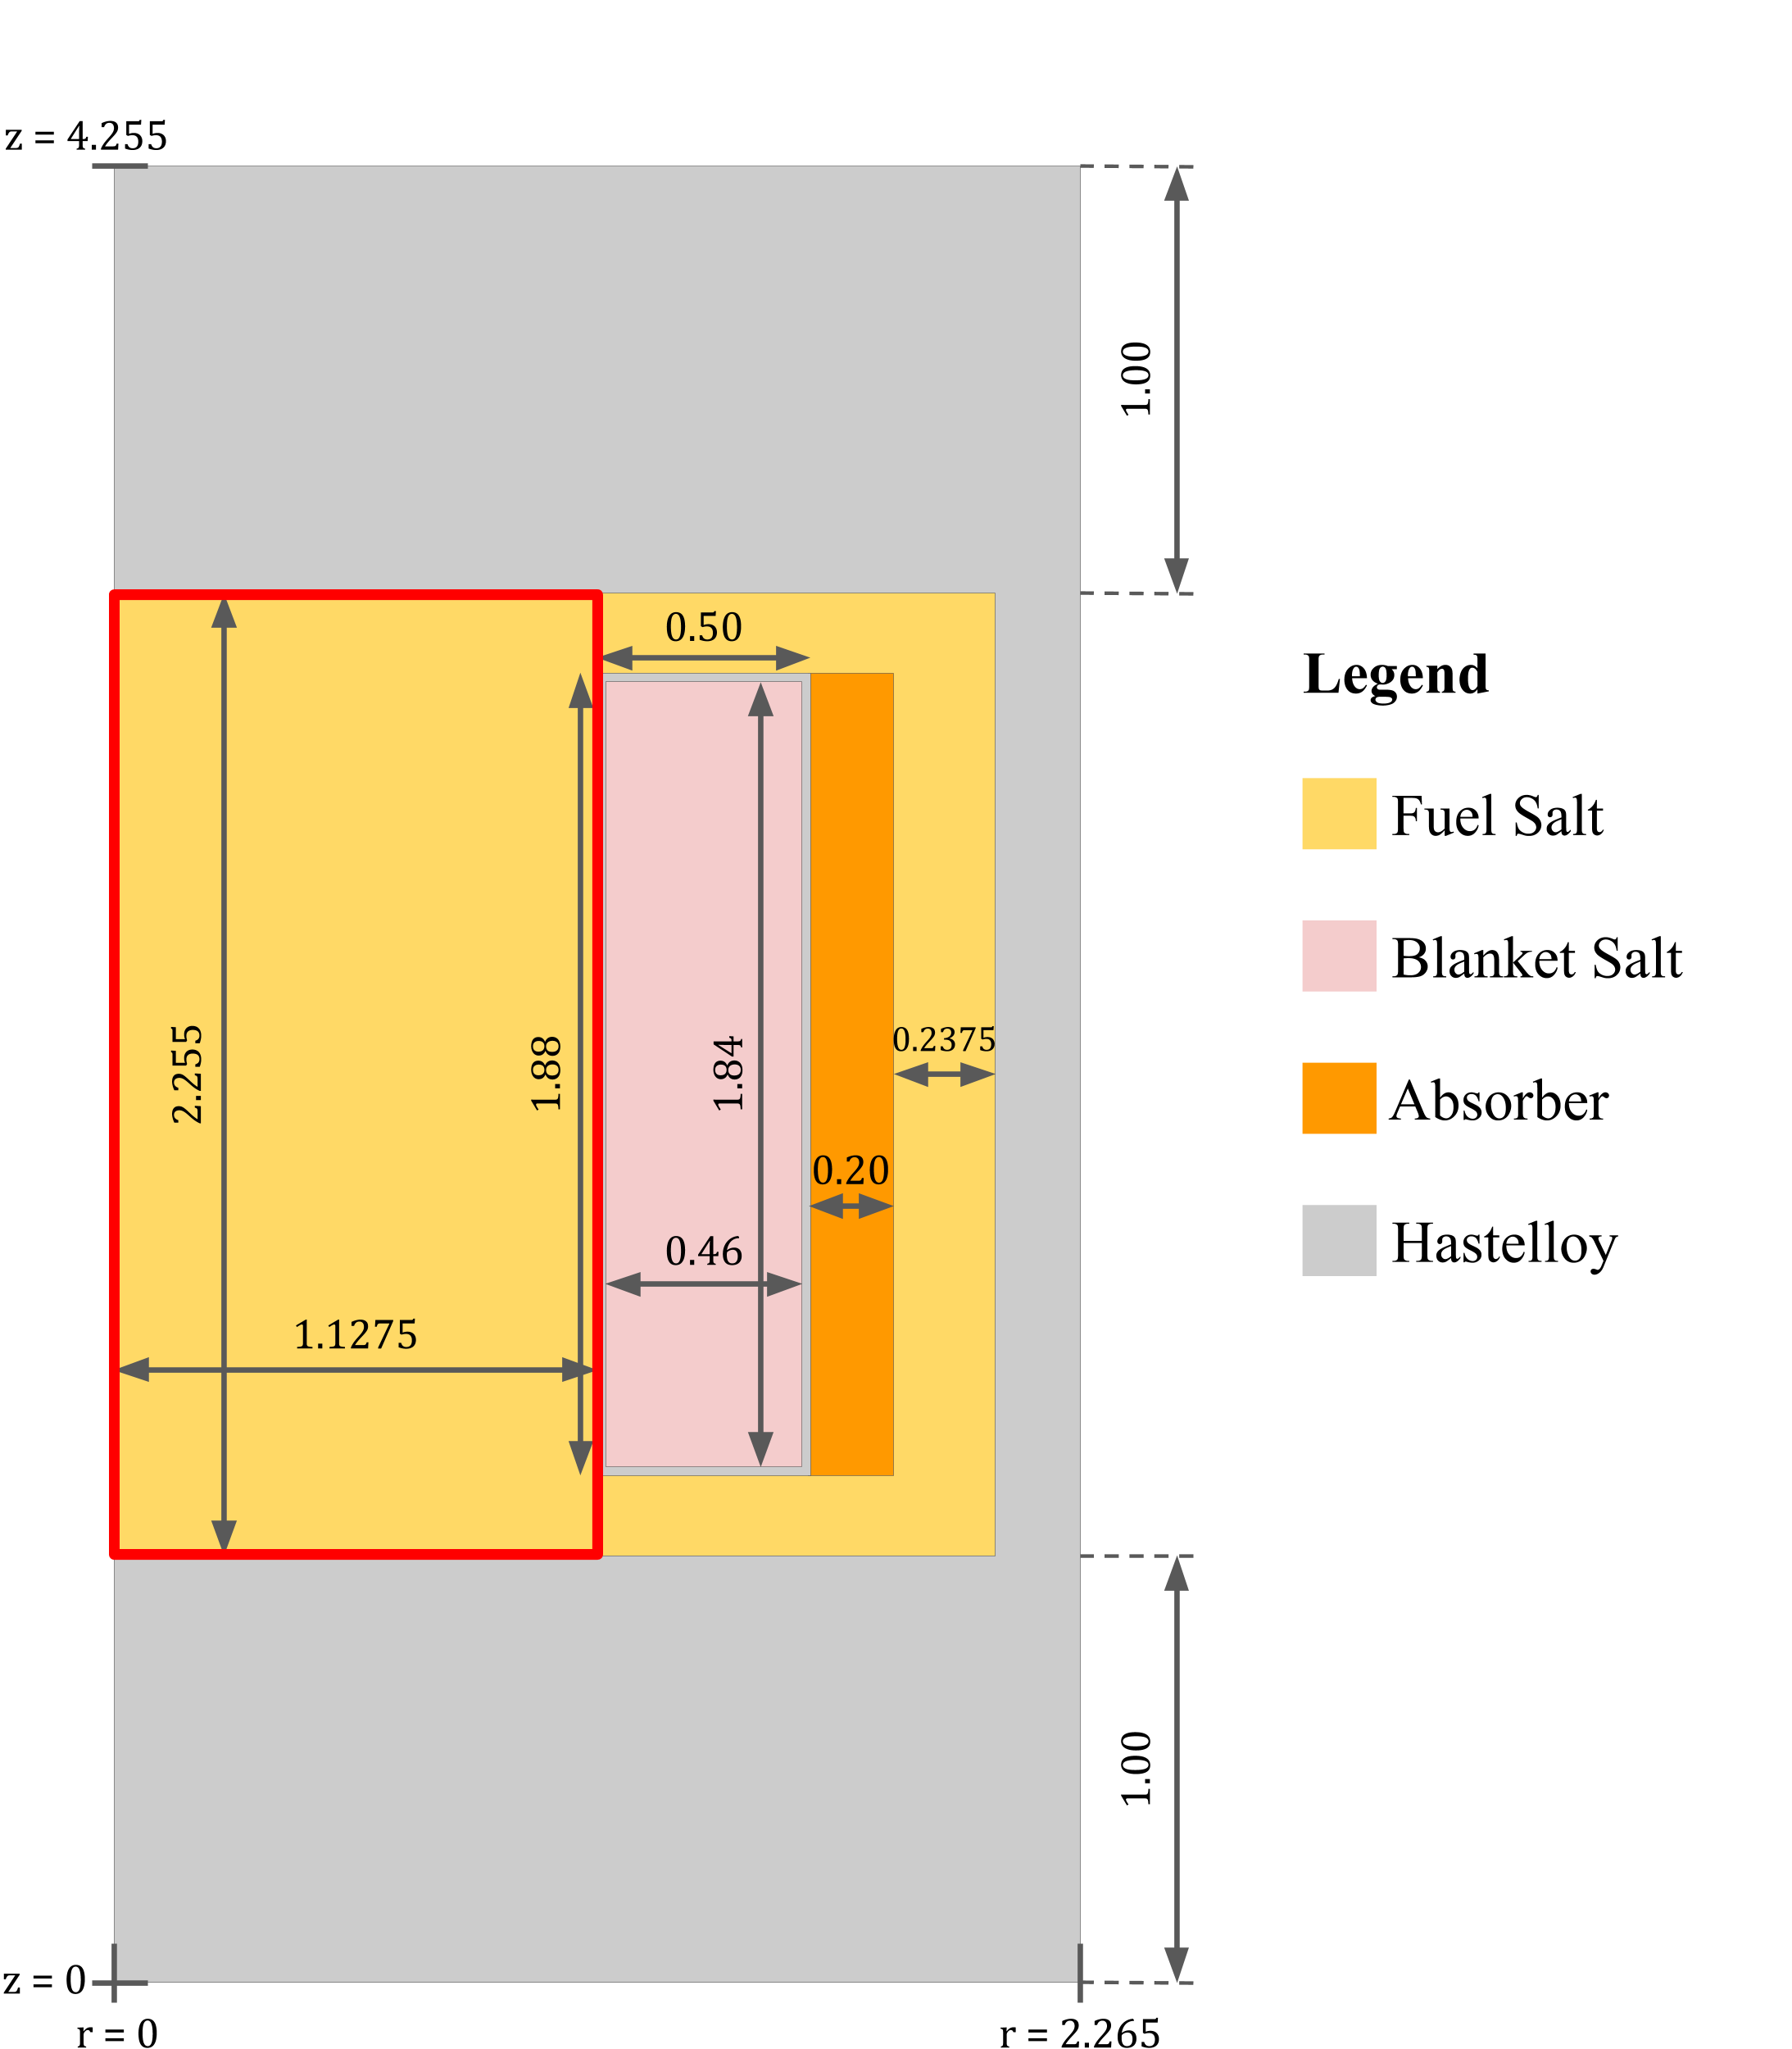
\includegraphics[width=.55\columnwidth]{central-core-legend}
	\caption{Schematic diagram of the 2-D axisymmetric \gls{MSFR} model with
	the core region enclosed by the red box \cite{park_advancement_2020}.}
	\label{fig:msfr-geometry}
\end{figure}

For the verification and demonstration of the capabilities introduced in this
work, I ran coupled steady-state and unprotected accident transient
simulations of the \gls{MSFR} and compared the results with published results
by Fiorina et al. \cite{fiorina_modelling_2014} and Aufiero et al.
\cite{aufiero_development_2014}. In this section, the PoliMi and TU Delft models
refer to two sets of results published by Fiorina et al. I compensated for
the lack of a turbulence model in Moltres by imposing a fixed turbulent
viscosity of 40 Pa$\cdot$s in addition to the molecular viscosity $\mu$ in
Equation \ref{eq:momemtum}. Figure \ref{fig:msfr-geometry} shows the 2-D
axisymmetric \gls{MSFR} model with the core region indicated with the red box,
while the rest of the fuel region was modeled with the 1-D loop system. Fuel
salt flows into the core region from the inlet at the bottom-right corner and
out through the outlet at the top-right corner.

\begin{figure}[htb!]
    \centering
    \begin{subfigure}[t]{.35\textwidth}
        \centering
        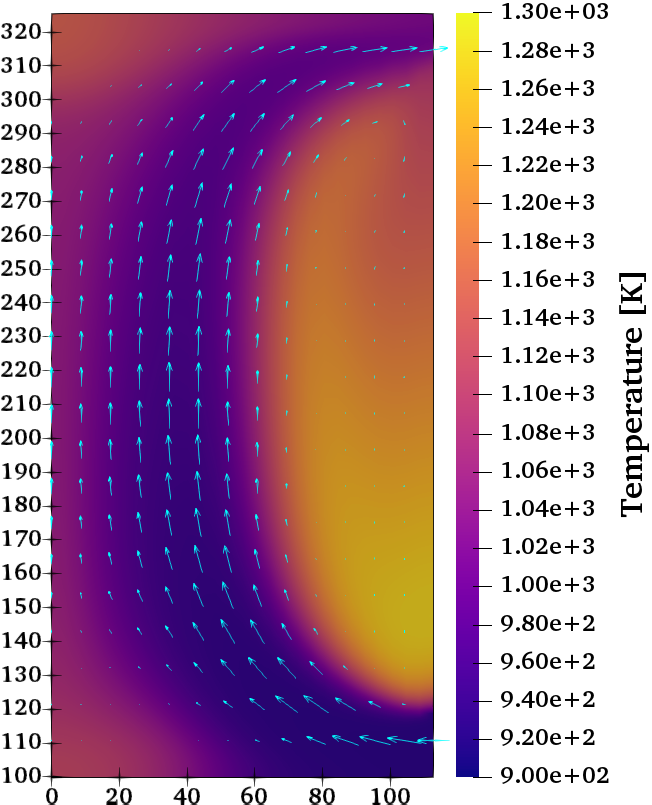
\includegraphics[width=\textwidth]{flow-temp-plasma}
    \end{subfigure}
    \hfill
    \begin{subfigure}[t]{.625\textwidth}
        \centering
        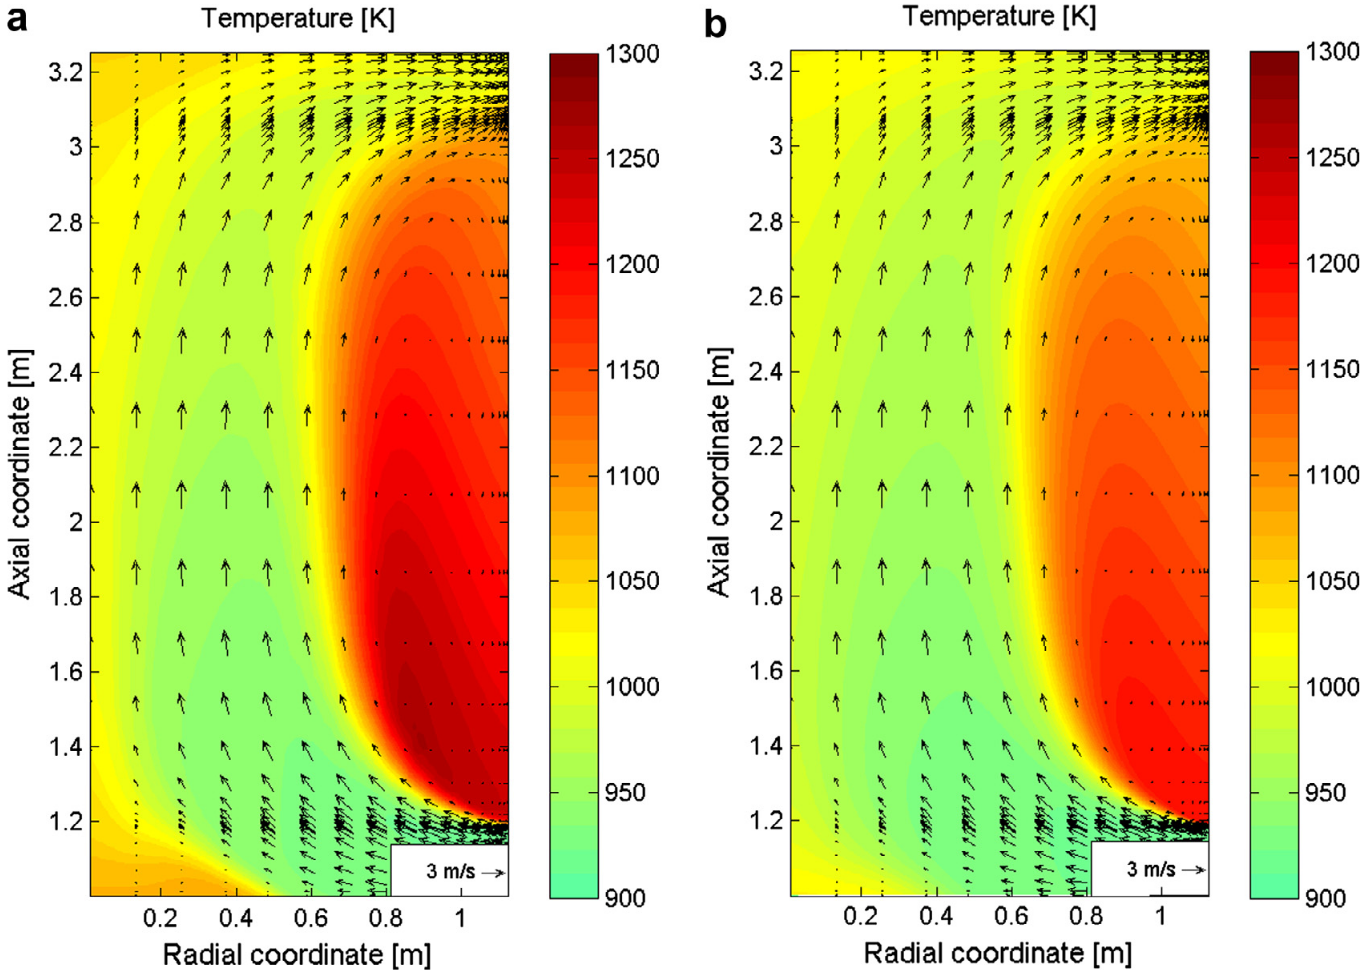
\includegraphics[width=\textwidth]{flow-temp-fiorina}
    \end{subfigure}
    \caption{Temperature and velocity fields in the core from Moltres
    (left), PoliMi (center), and TU Delft (right) models. The colors represent
    temperature according to the respective color bars and the arrows
    represent velocity fields. \cite{park_advancement_2020}}
    \label{fig:flow-temp}
\end{figure}

Figure \ref{fig:flow-temp} shows the core steady-state temperature and velocity
fields from the Moltres, PoliMi, and TU Delft models. The Moltres
model showed
good qualitative agreement with the PoliMi and TU Delft models since the plots
show similar flow and hotspot features in all three models. The salt flow
follows a parabolic path from the inlet to the outlet. A large
recirculation region formed near the right wall while the top and bottom
regions along the central axis experience relatively stagnant flow compared to
the main salt flow stream. The temperature hotspots coincide with the regions of
recirculation and stagnation because convection is the dominant heat transfer
mechanism. Maximum temperatures are observed near the bottom of the
recirculation zones; the Moltres model reports 1275 K, which is closer to the
PoliMi model ($\sim1300$ K) than the TU Delft model ($\sim1200$ K). Thus, the
incompressible flow model in Moltres performed well in reproducing the
thermal-hydraulic profiles of the \gls{MSFR} under steady-state conditions
despite the fixed turbulent viscosity assumption.

\begin{figure}[b!]
    \centering
    \begin{subfigure}[t]{.30\textwidth}
        \centering
        \vspace{.9cm}
        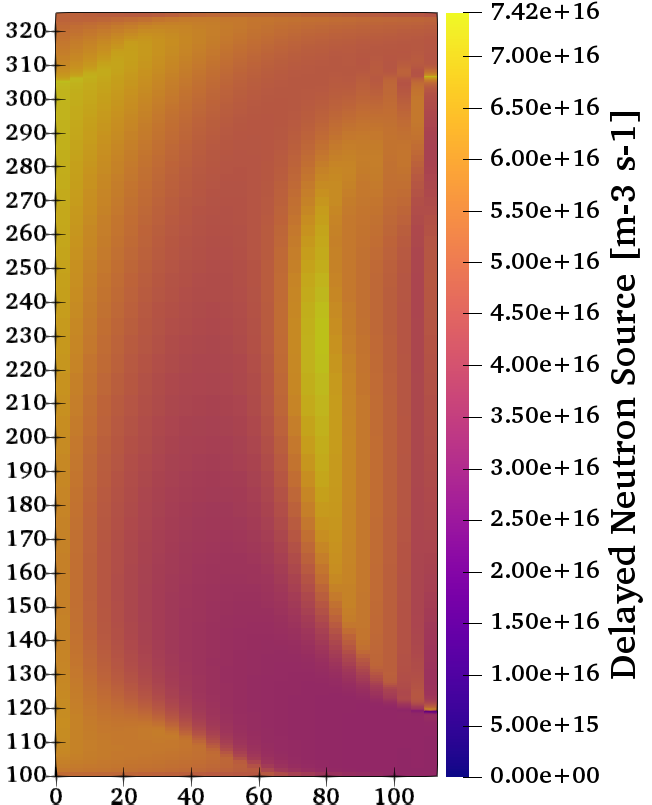
\includegraphics[width=\textwidth]{pre}
    \end{subfigure}
    \begin{subfigure}[t]{.69\textwidth}
        \centering
        \vspace{0pt}
        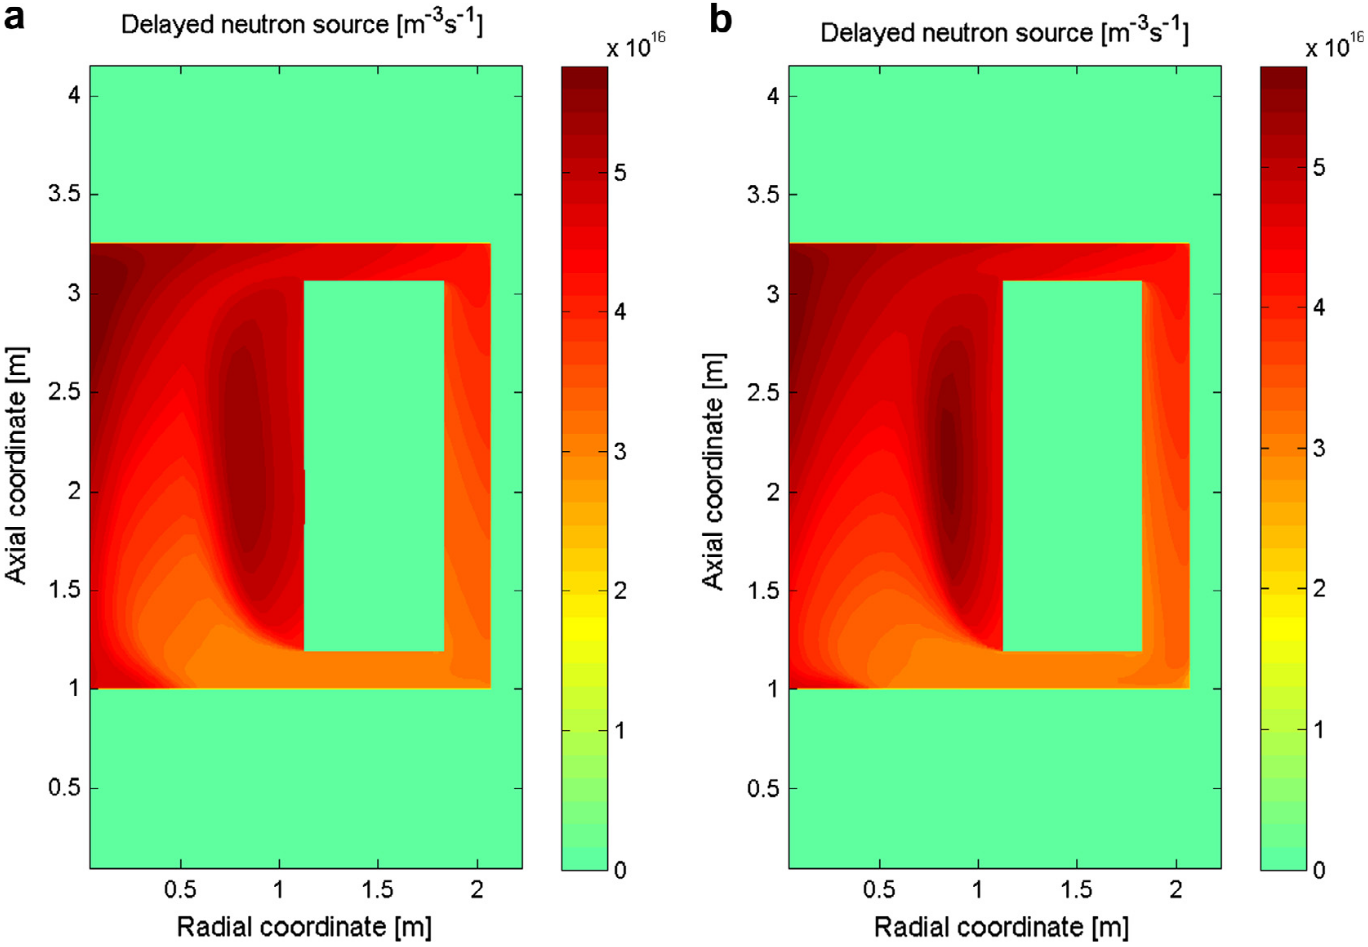
\includegraphics[width=\textwidth]{fiorina-pre}
    \end{subfigure}
    \caption{Total delayed neutron source distribution in the core from the
    Moltres (left), PoliMi (center), and TU Delft (right) models.}
    \label{fig:pre}
\end{figure}

Moltres reported a peak total neutron flux of $9.80 \times 10^{15}$
cm$^{-2}\cdot$s$^{-1}$, which is close to the 8.6 and 9.0 $\times 10^{15}$
cm$^{-2}\cdot$s$^{-1}$ values reported by Fiorina et al.
\cite{fiorina_molten_2013} and \cite{aufiero_development_2014}. However, the
delayed neutron source distribution from the Moltres model exhibits some
differences compared to the PoliMi and TU Delft models, as shown in Figure
\ref{fig:pre}. The Moltres model retains fewer precursors than the other two
models, resulting in a higher 44.16\% out-of-core delayed neutron emissions
compared with the 34.80\% and 34.85\% from the other models
\cite{park_advancement_2020}. Therefore, the incompressible flow model with
constant turbulent viscosity fell short of accurately capturing precursor
drift in the \gls{MSFR}.

\begin{figure}[htb]
    \centering
    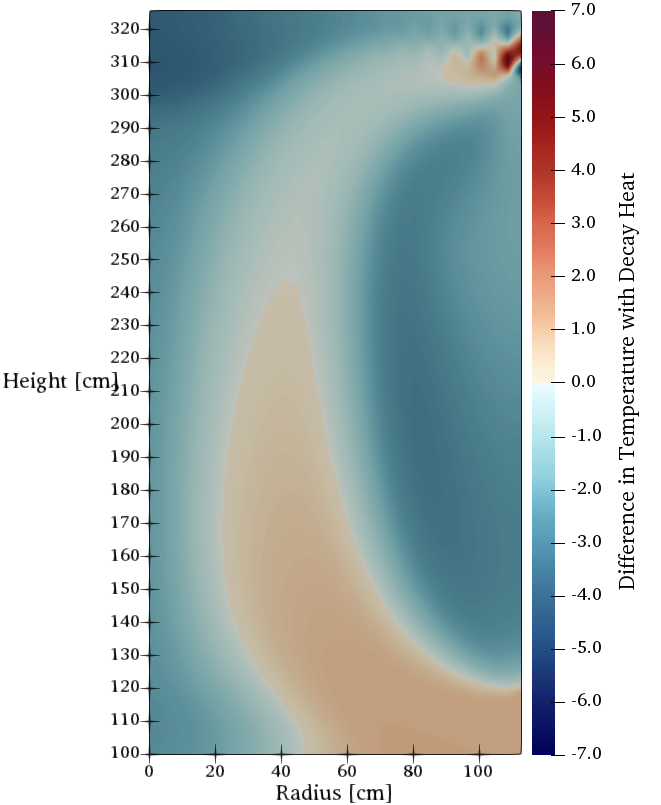
\includegraphics[width=.5\textwidth]{decay-heat-temp}
    \caption{Difference in core temperatures at steady-state with decay heat
    relative to the result without decay heat (Figure \ref{fig:flow-temp}).}
    \label{fig:decayheattemp}
\end{figure}

This work also compared steady-state temperature distributions with and without
the decay heat model. As expected, the decay heat model effectively flattens
the heat source distribution, reducing the maximum
temperatures and increasing the minimum temperatures observed in the model.
Figure \ref{fig:decayheattemp} shows a decrease in temperature in the hotspot
regions and an increase in temperature near the inlet, the coolest
region in the core.

For the transient studies, this work considered unprotected reactivity
insertion, loss-of-heat-sink, loss-of-flow, and pump-overspeed accidents. The
term ``unprotected'' signifies accident scenarios without reactor SCRAM.
Moltres reproduced similar trends observed in the PoliMi and TU Delft
models for the reactivity insertion and loss-of-heat-sink scenarios. For
instance, Figure \ref{fig:200pcmheat} shows the power output response of the
three models following a 200 pcm step reactivity insertion. The lower peak from
the Moltres model is attributed to the stronger negative fuel temperature
reactivity feedback coefficient of $-7.184$ pcm$\cdot$K$^{-1}$ compared to
approximately $-6.5$ pcm$\cdot$K$^{-1}$ for the PoliMi and TU Delft models.

\begin{figure}[htb!]
    \centering
    \begin{minipage}[b]{.49\textwidth}
      \centering
      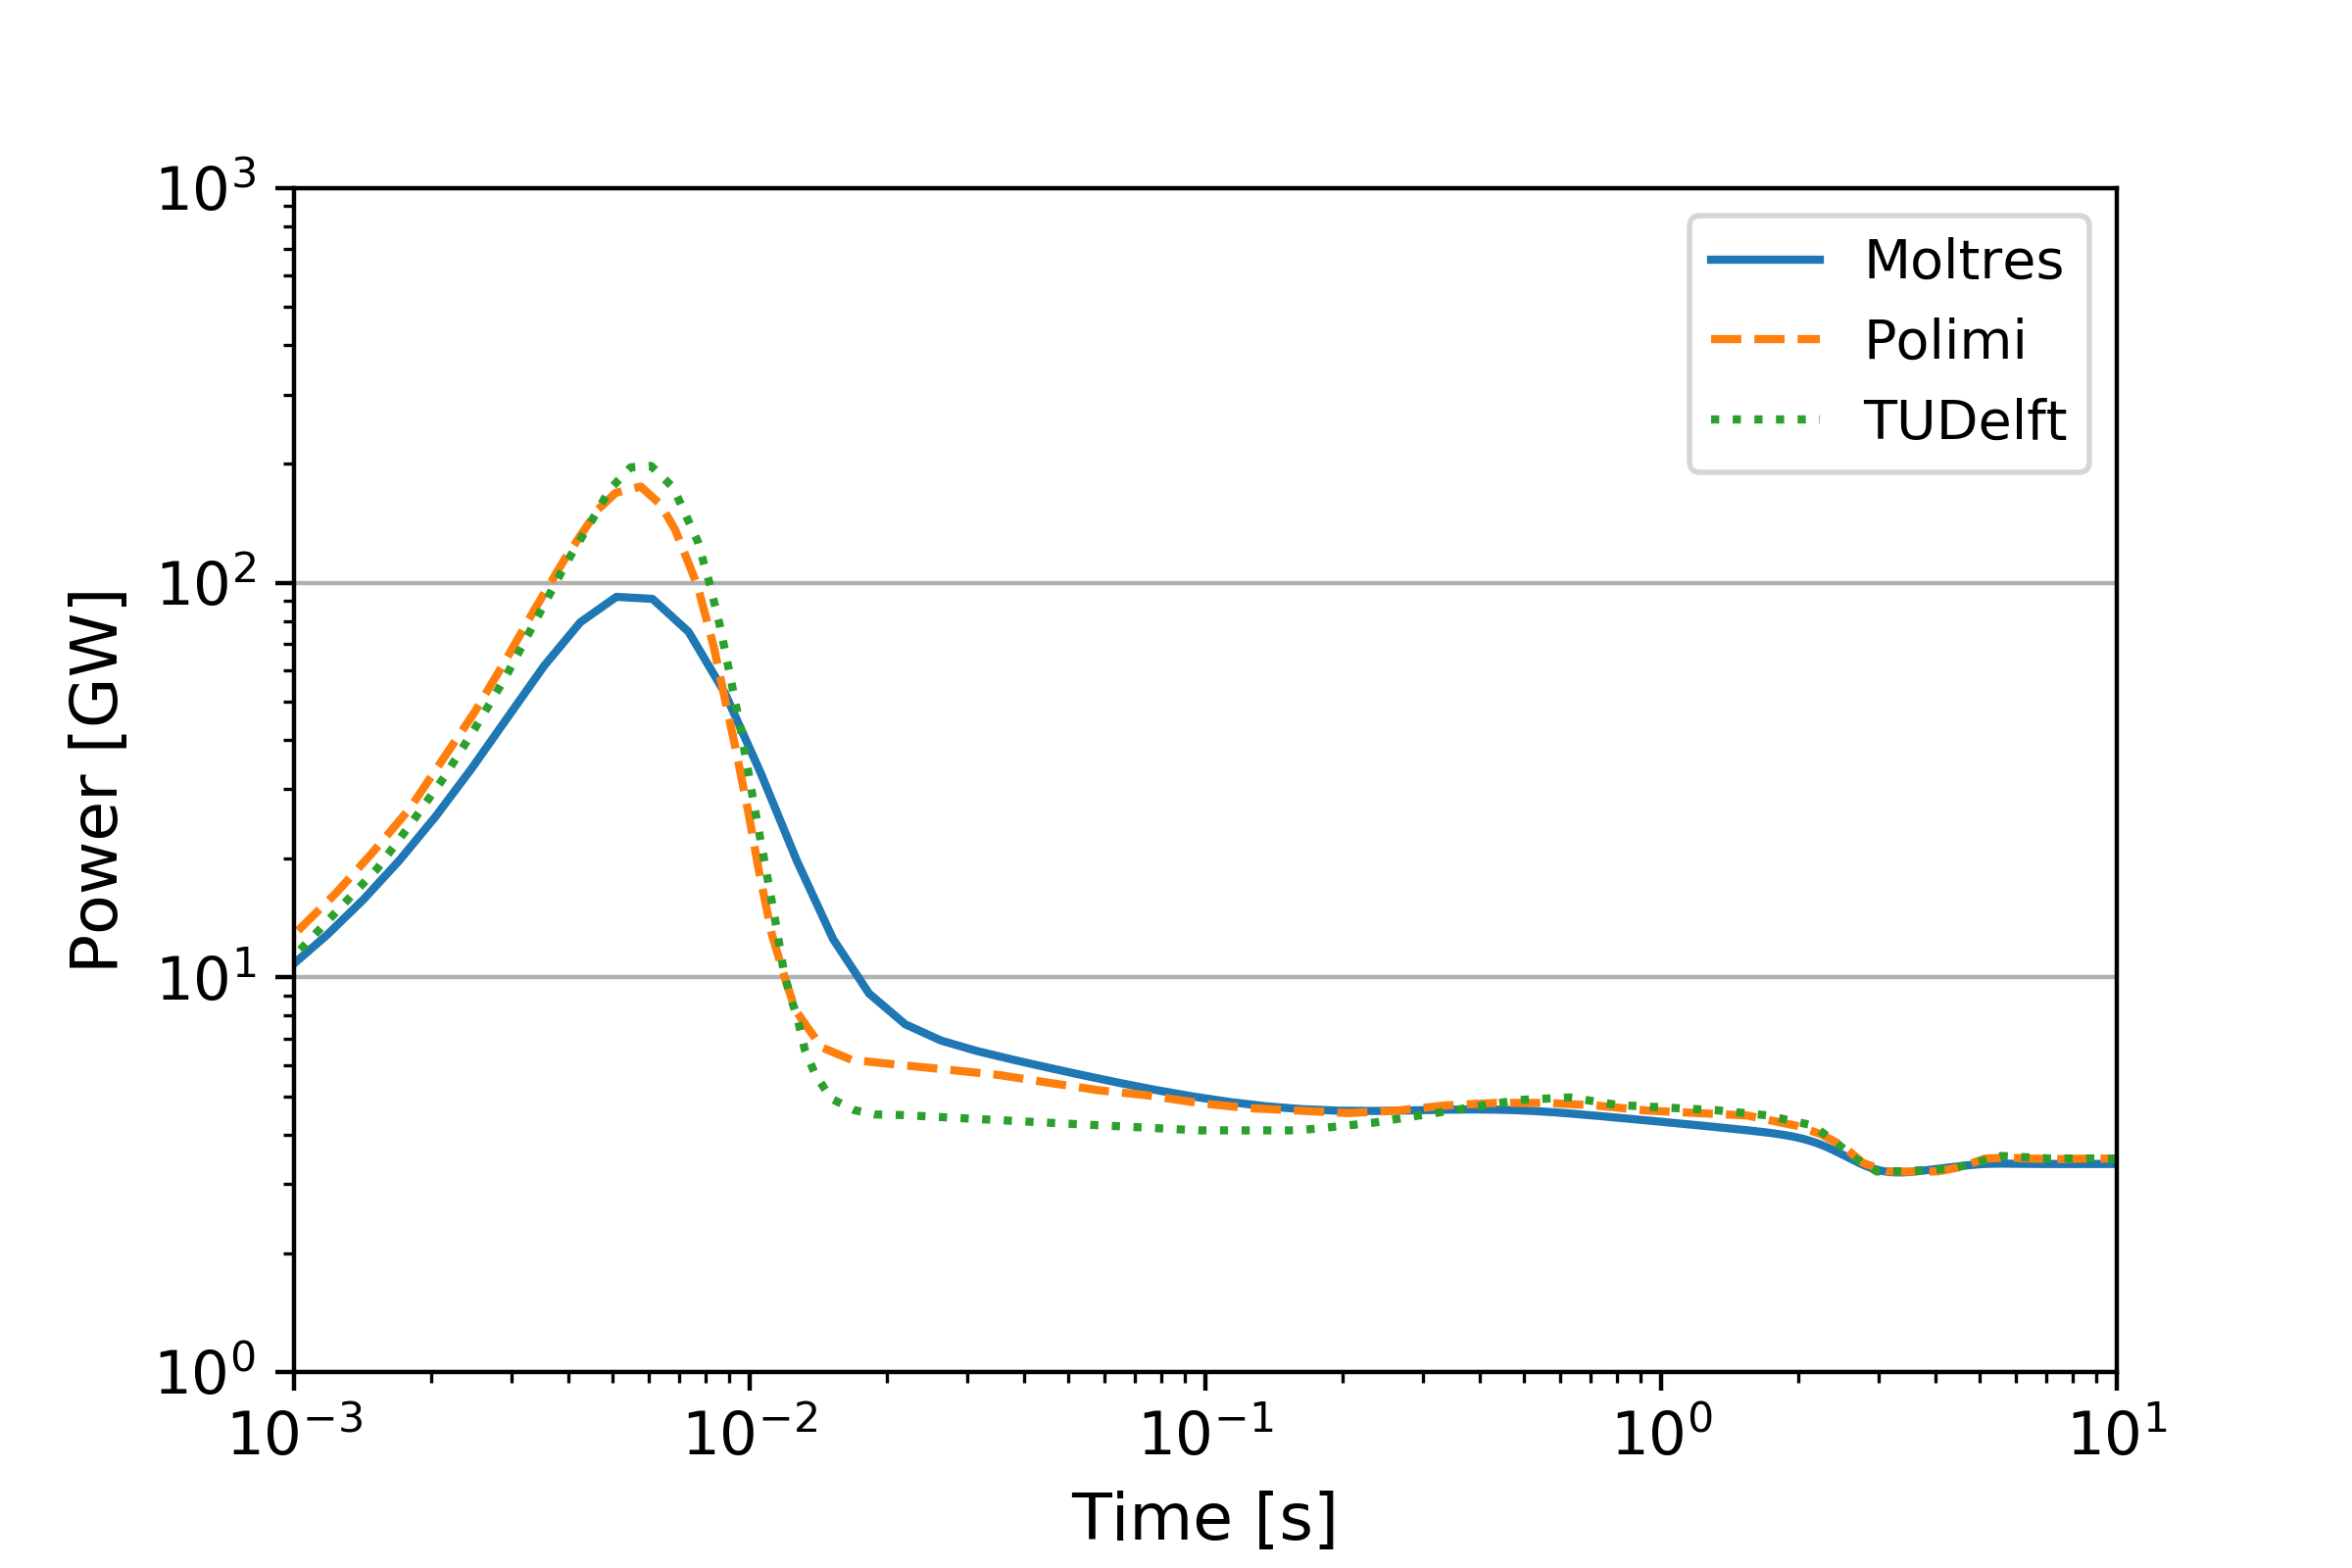
\includegraphics[width=\textwidth]{200pcm-heat}
      \caption{Power output following a 200 pcm step-wise unprotected reactivity
        insertion in the Moltres, PoliMi, and
        TU Delft models \cite{fiorina_modelling_2014}.}
      \label{fig:200pcmheat}
    \end{minipage}
    \hfill
    \begin{minipage}[b]{.49\textwidth}
      \centering
      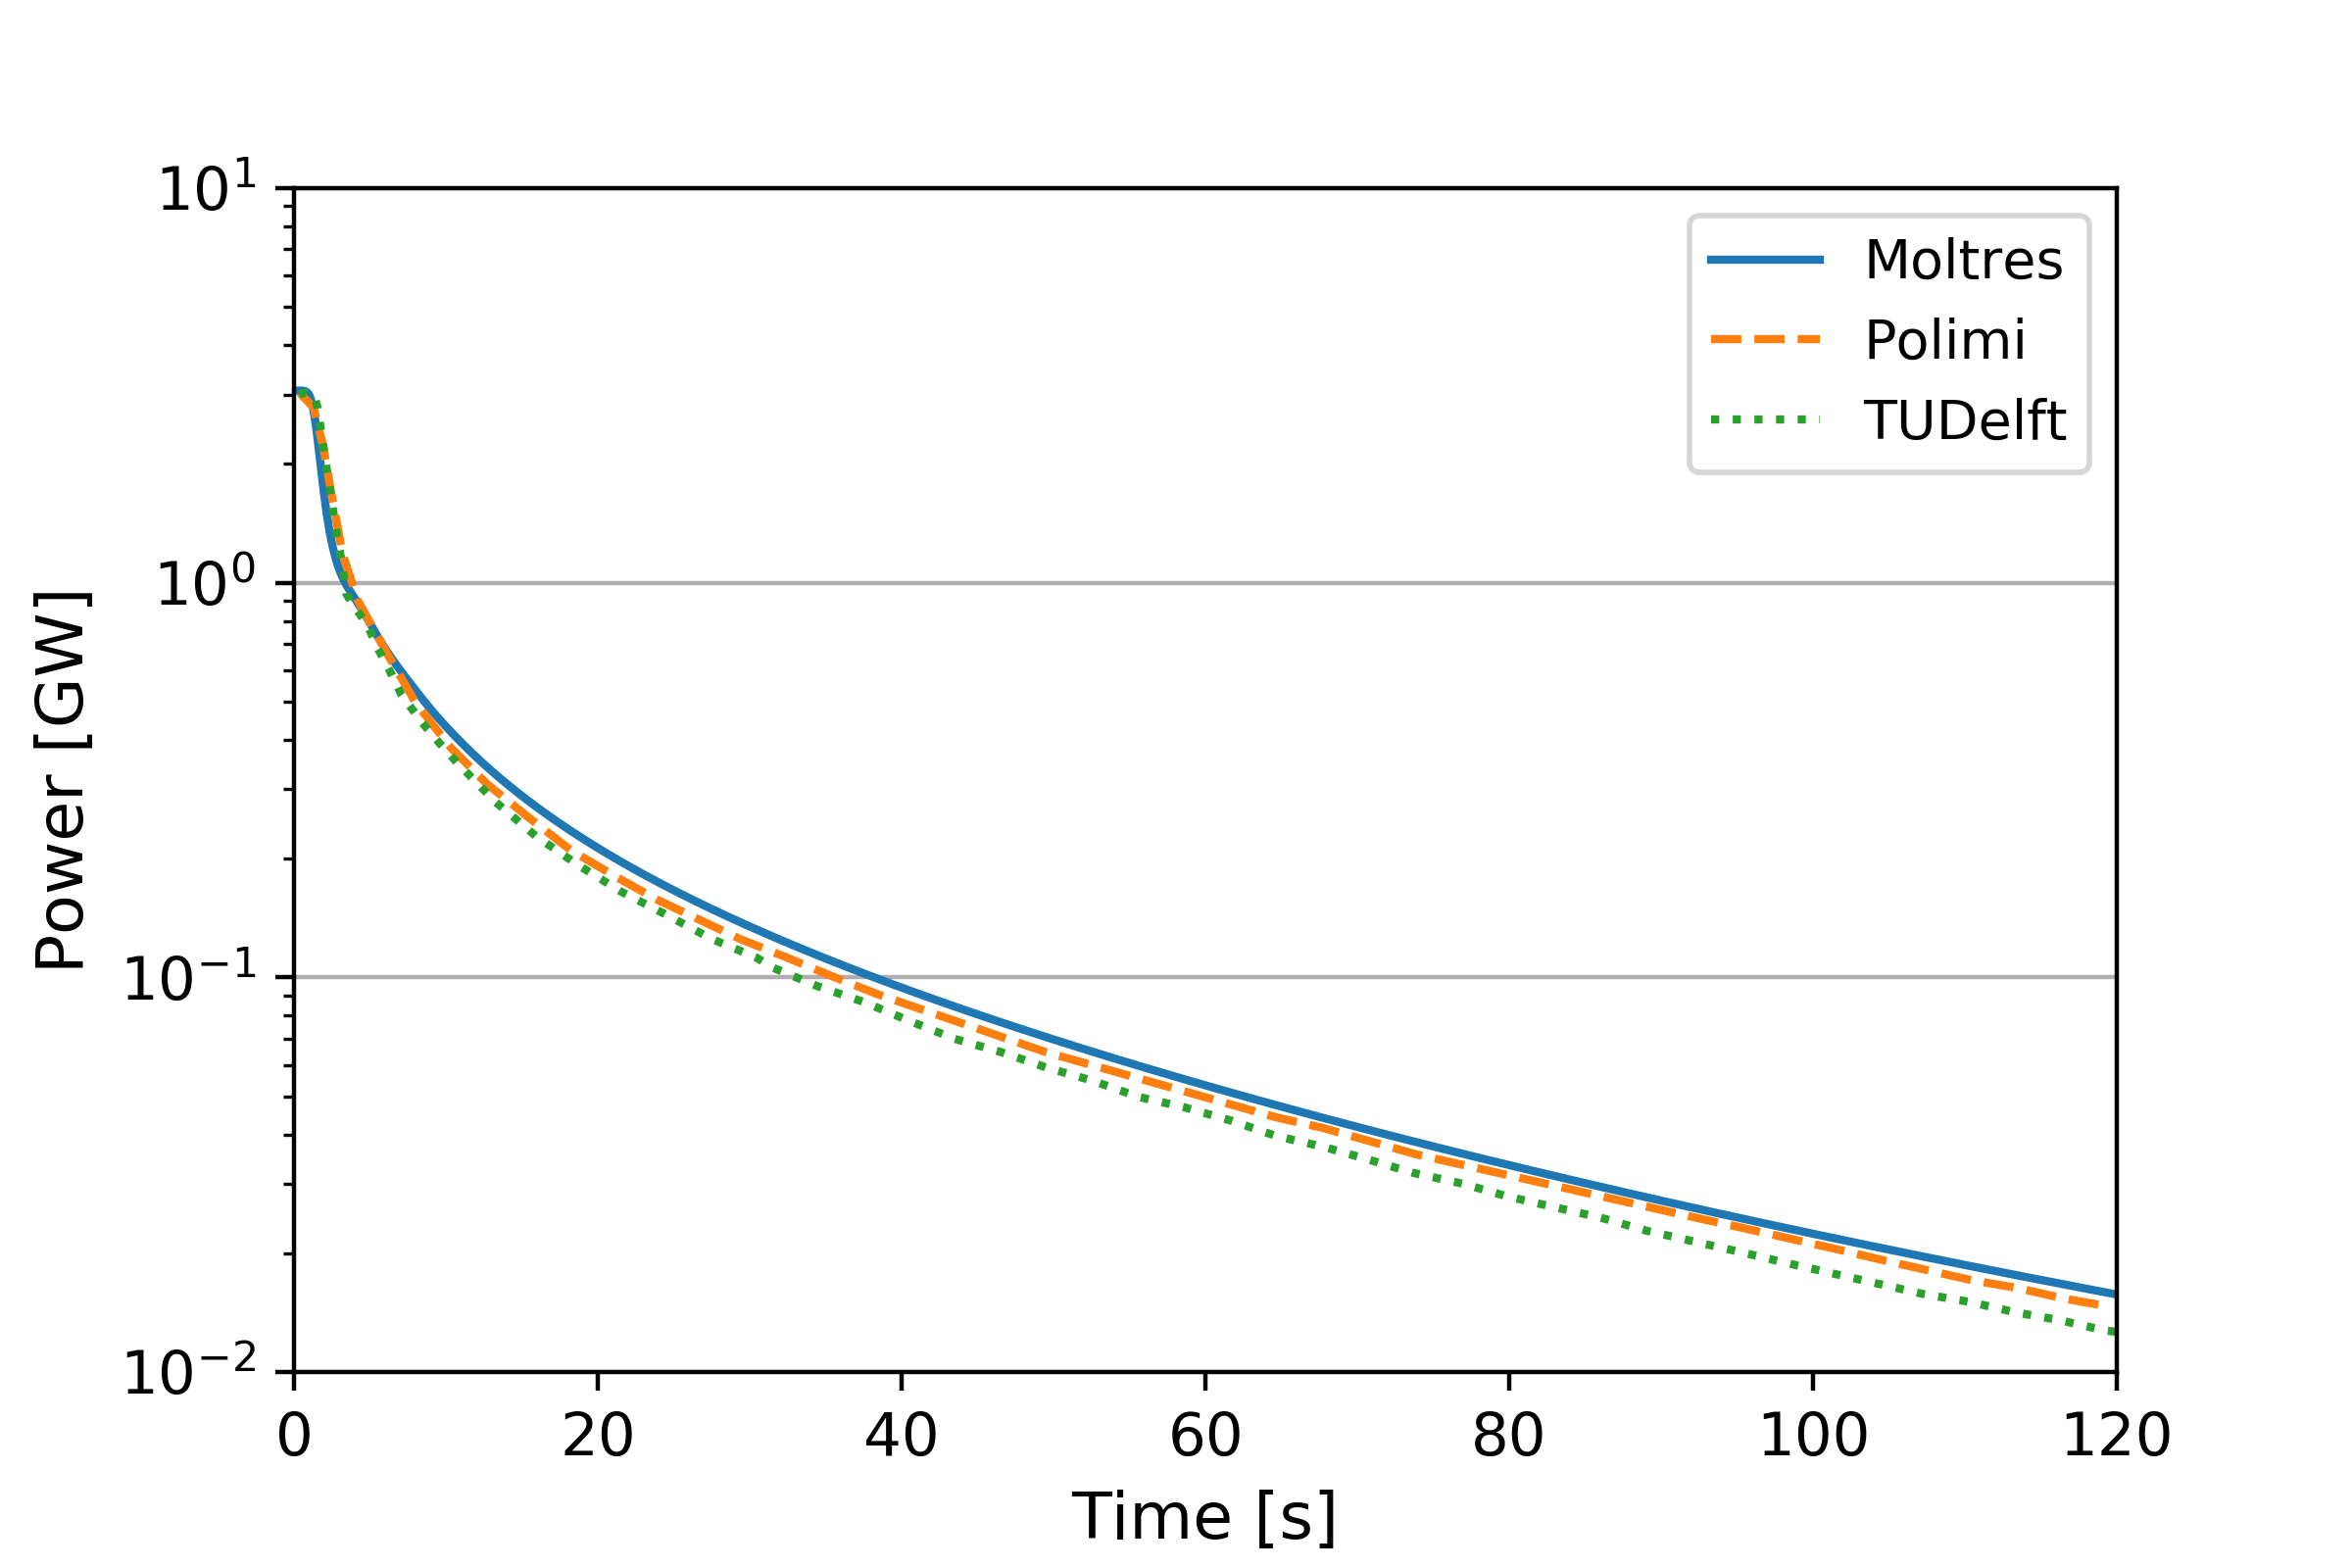
\includegraphics[width=\textwidth]{lohs-heat}
      \caption{Power output during
        an unprotected loss of heat sink transient in the Moltres, PoliMi, and
        TU Delft models \cite{fiorina_modelling_2014} without decay heat.}
      \label{fig:lohsheat}
    \end{minipage}
\end{figure}

The loss-of-heat-sink transients were performed with and without the decay heat
model because the TU Delft model did not possess this capability. As shown in
Figure \ref{fig:lohsheat}, without decay heat, all three models reported
similar power output responses following the loss of cooling through the heat
exchanger modeled as an exponential decrease in heat removal rate with a time
constant of 1 s. As prompt heat generation decreases due to rising core
temperatures and the negative temperature reactivity feedback, decay heat
becomes a significant heat source. We observe this in Figure
\ref{fig:moltresdecaypower}, which shows decay heat output overtaking prompt
heat output 34 s into the accident scenario. With the decay heat model, the
Moltres model shows good agreement with the PoliMi model. The temperature
increase averaged over the fuel salt loop falls within 10\% of the PoliMi
model (Figure \ref{fig:polimidecaytemp}).

\begin{figure}[htb!]
	\centering
	\begin{minipage}[t]{0.485\columnwidth}
	    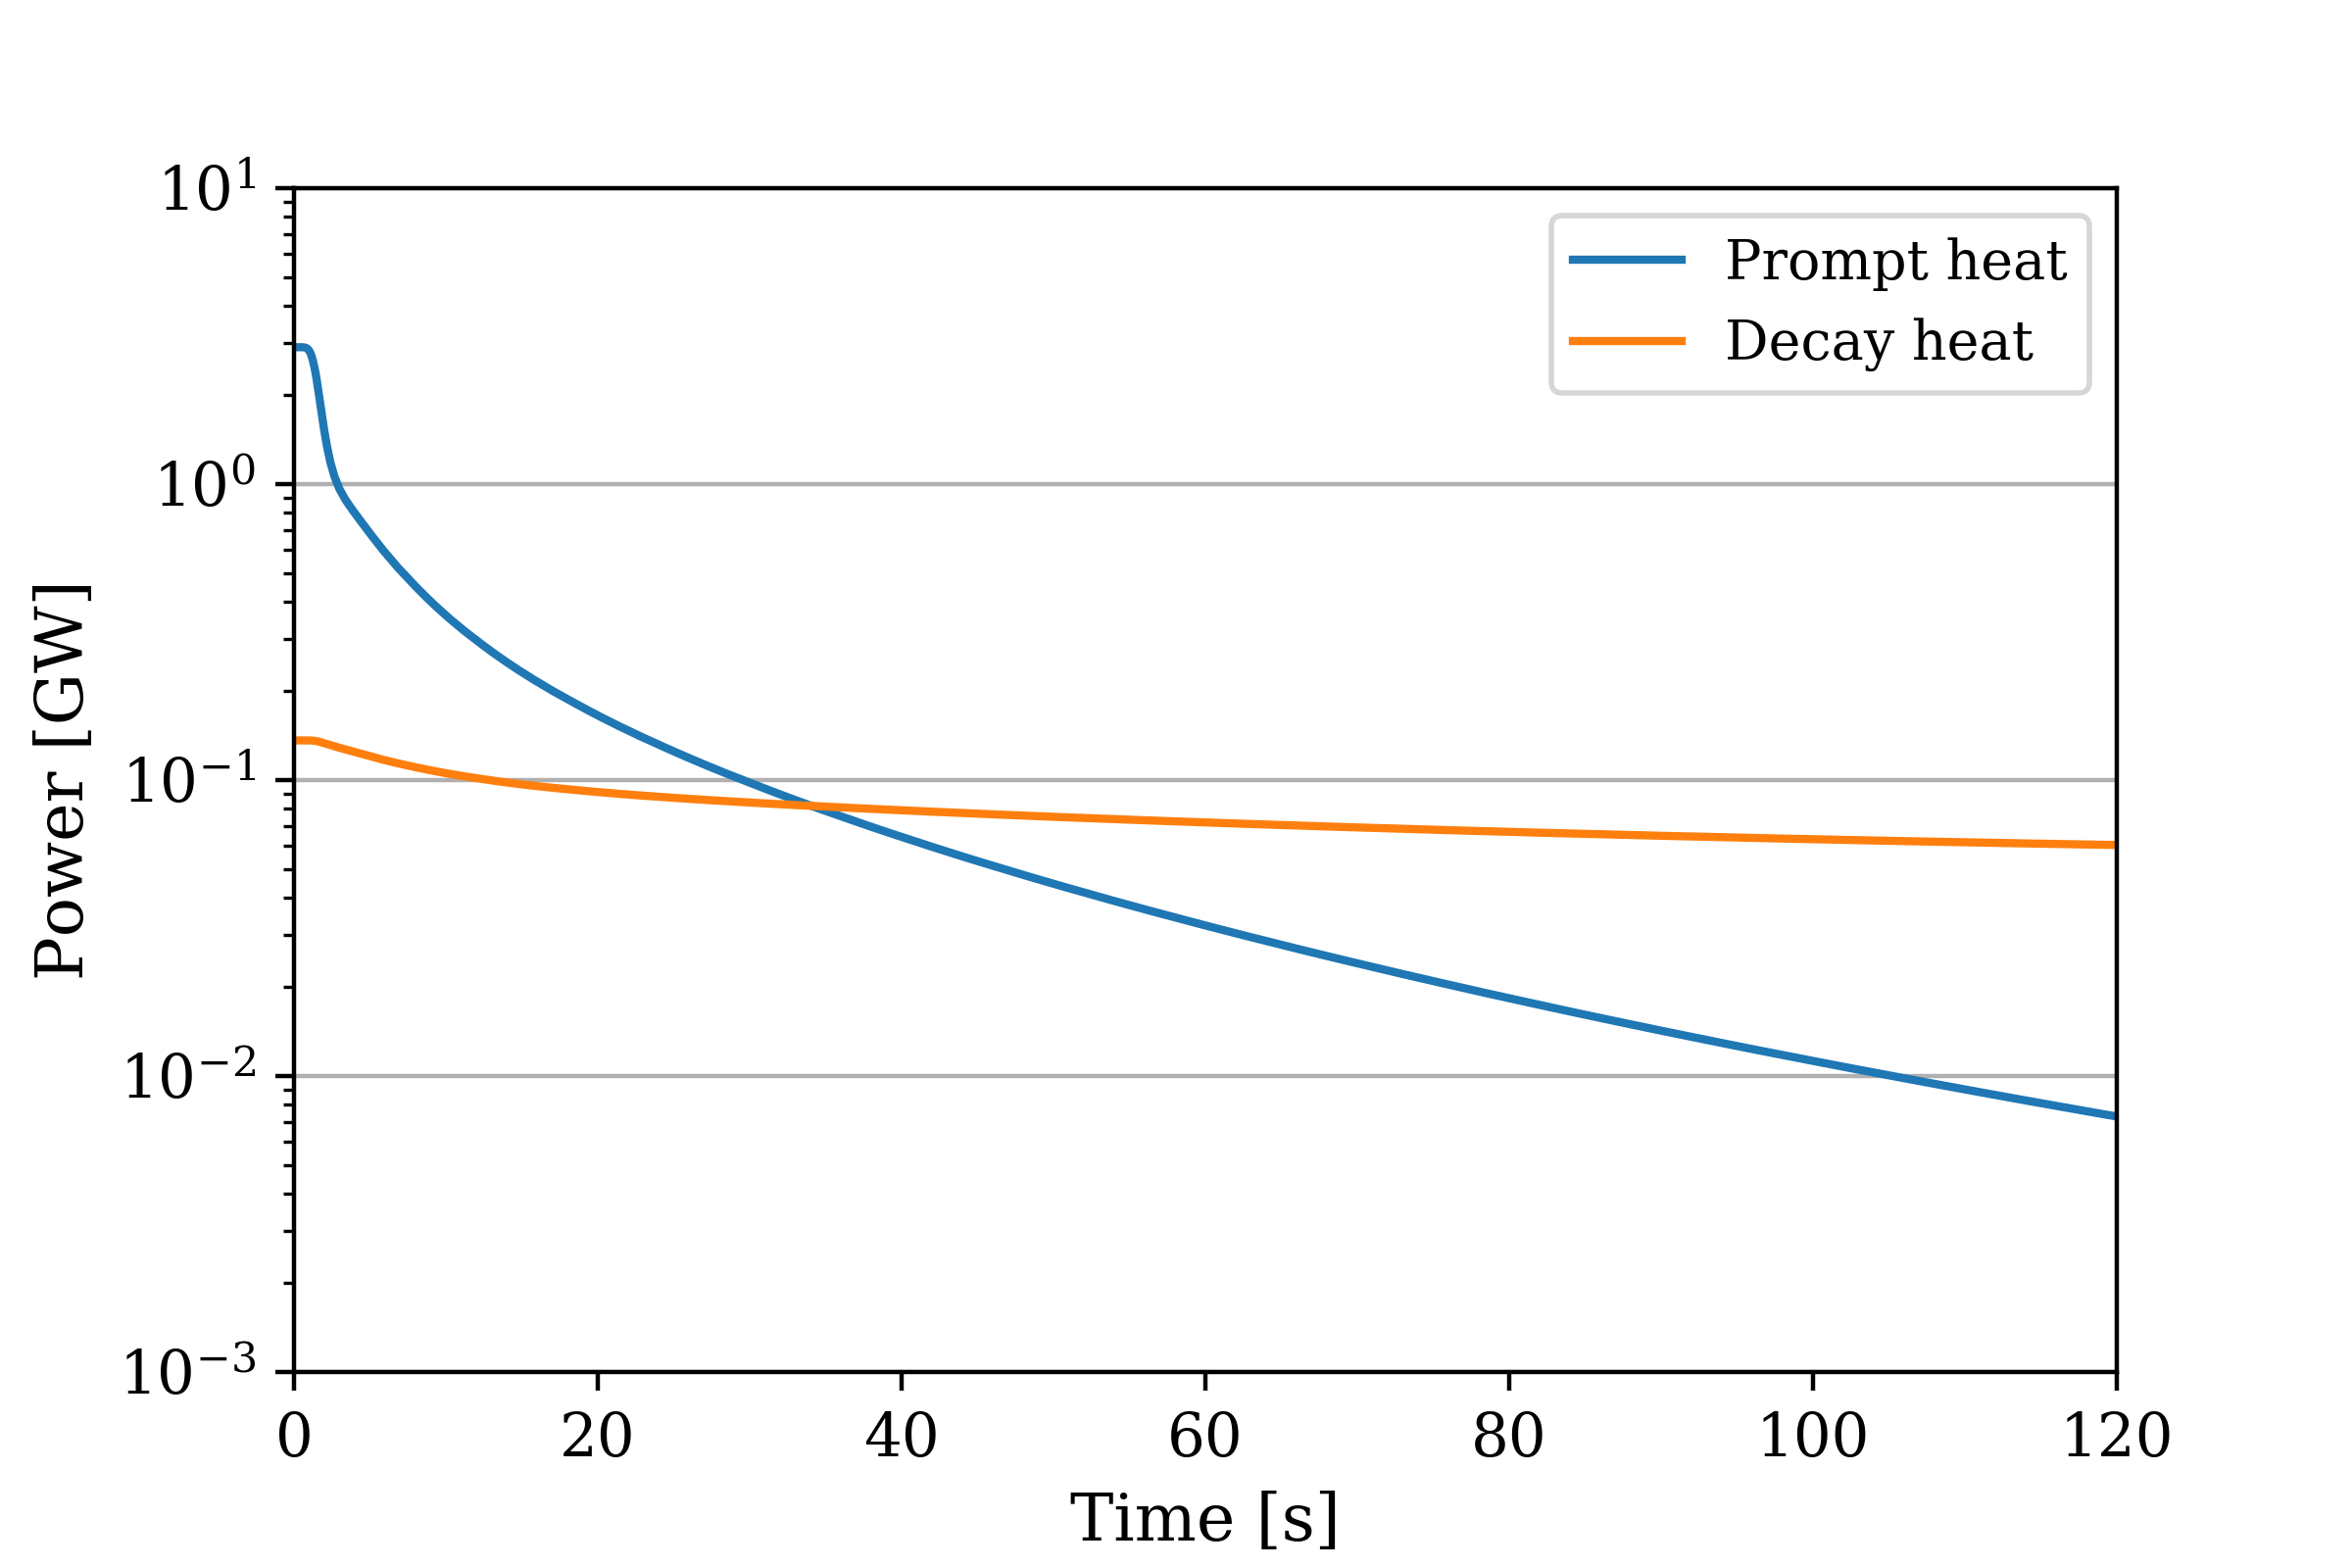
\includegraphics[width=\columnwidth]{moltres-decay-power}
	    \caption{Power output during
    an unprotected loss of heat sink transient in the Moltres model with
    decay heat.}
	    \label{fig:moltresdecaypower}
	\end{minipage}
	\hfill
	\begin{minipage}[t]{0.485\columnwidth}
	    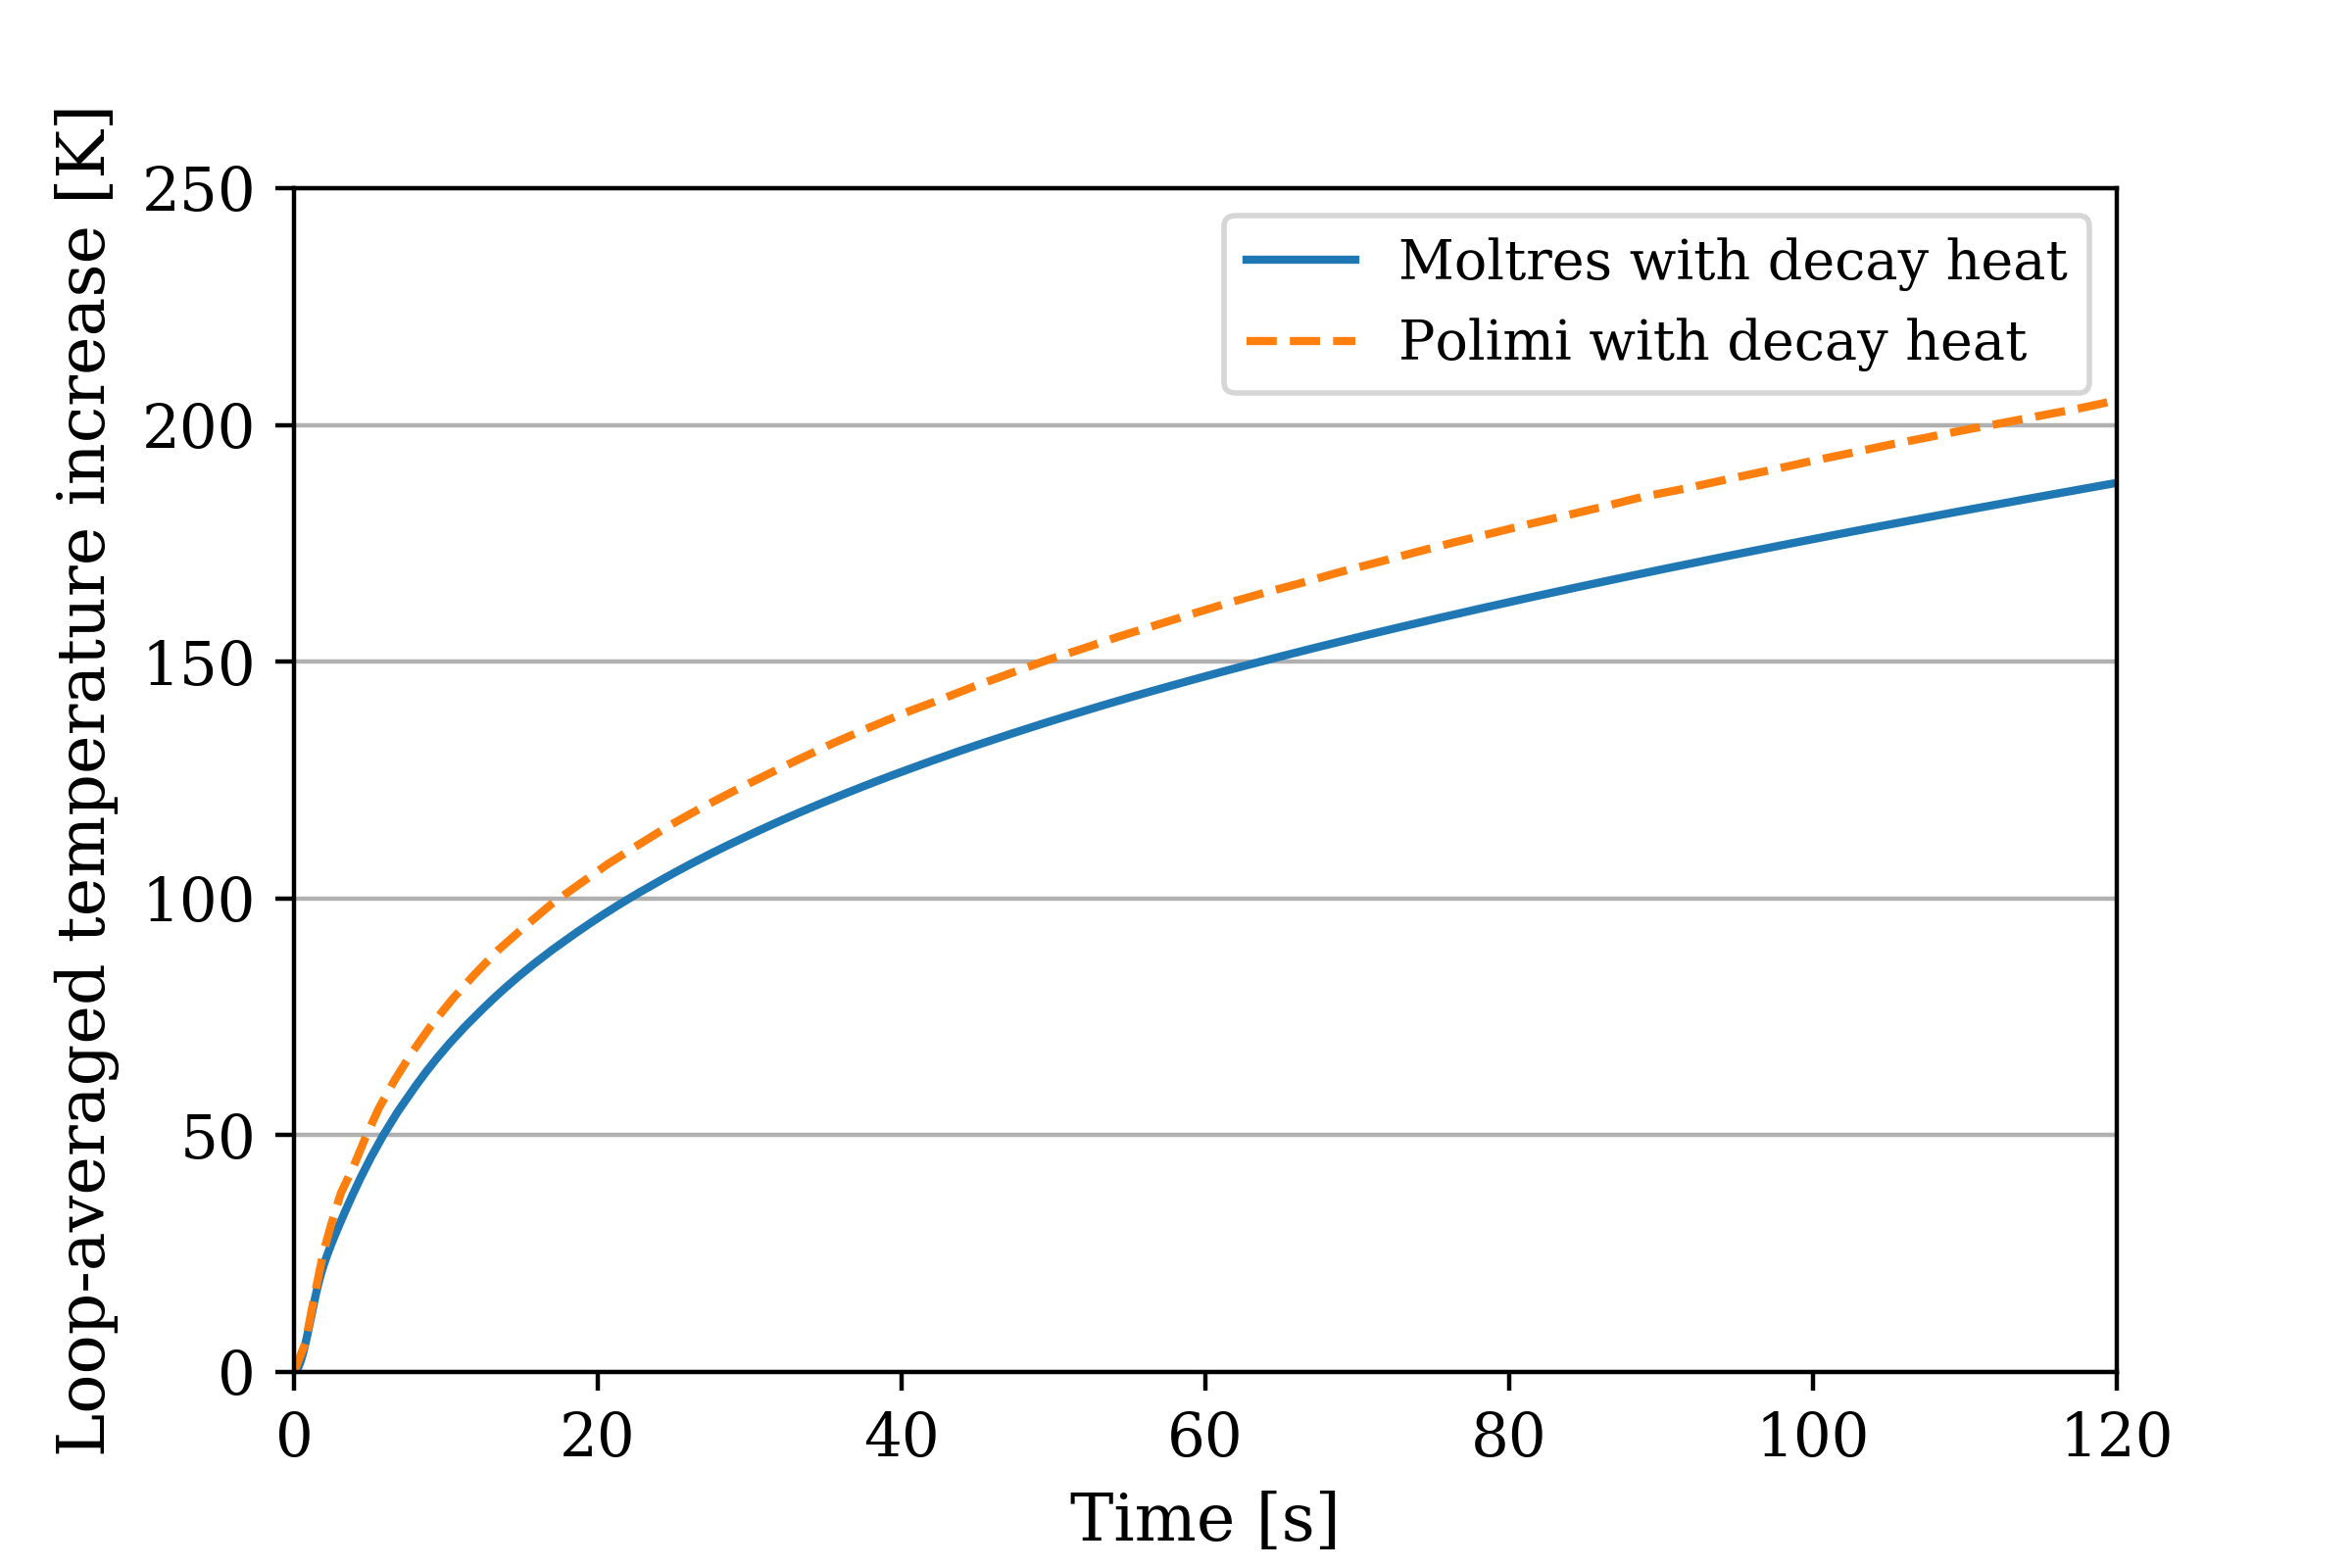
\includegraphics[width=\columnwidth]{decay-temp}
	    \caption{Loop-averaged temperature increase during
    an unprotected loss of heat sink transient in the Moltres and PoliMi
    models \cite{fiorina_modelling_2014} with decay heat.}
	    \label{fig:polimidecaytemp}
	\end{minipage}
\end{figure}

On the other hand, for the pump-initiated accident scenarios, significant
changes in the flow affected the validity of the uniform turbulent viscosity
assumption. These transients required ad hoc adjustments to the uniform
turbulent viscosity assumption as a function of volumetric flow to reproduce
the trends observed in the PoliMi and TU Delft models. Furthermore, unlike the
other two models, the Moltres model did not apply the Boussinesq approximation
for buoyancy-driven flow. The Moltres model could replicate expected trends in
the pump overspeed scenario (Figure \ref{fig:poshort}), but performed
poorly in the loss of flow scenario (Figure \ref{fig:lof}). In the latter
scenario, buoyancy effects become significant as the model loses forced flow.

\begin{figure}[htb!]
    \centering
    \begin{subfigure}[t]{.485\textwidth}
        \centering
        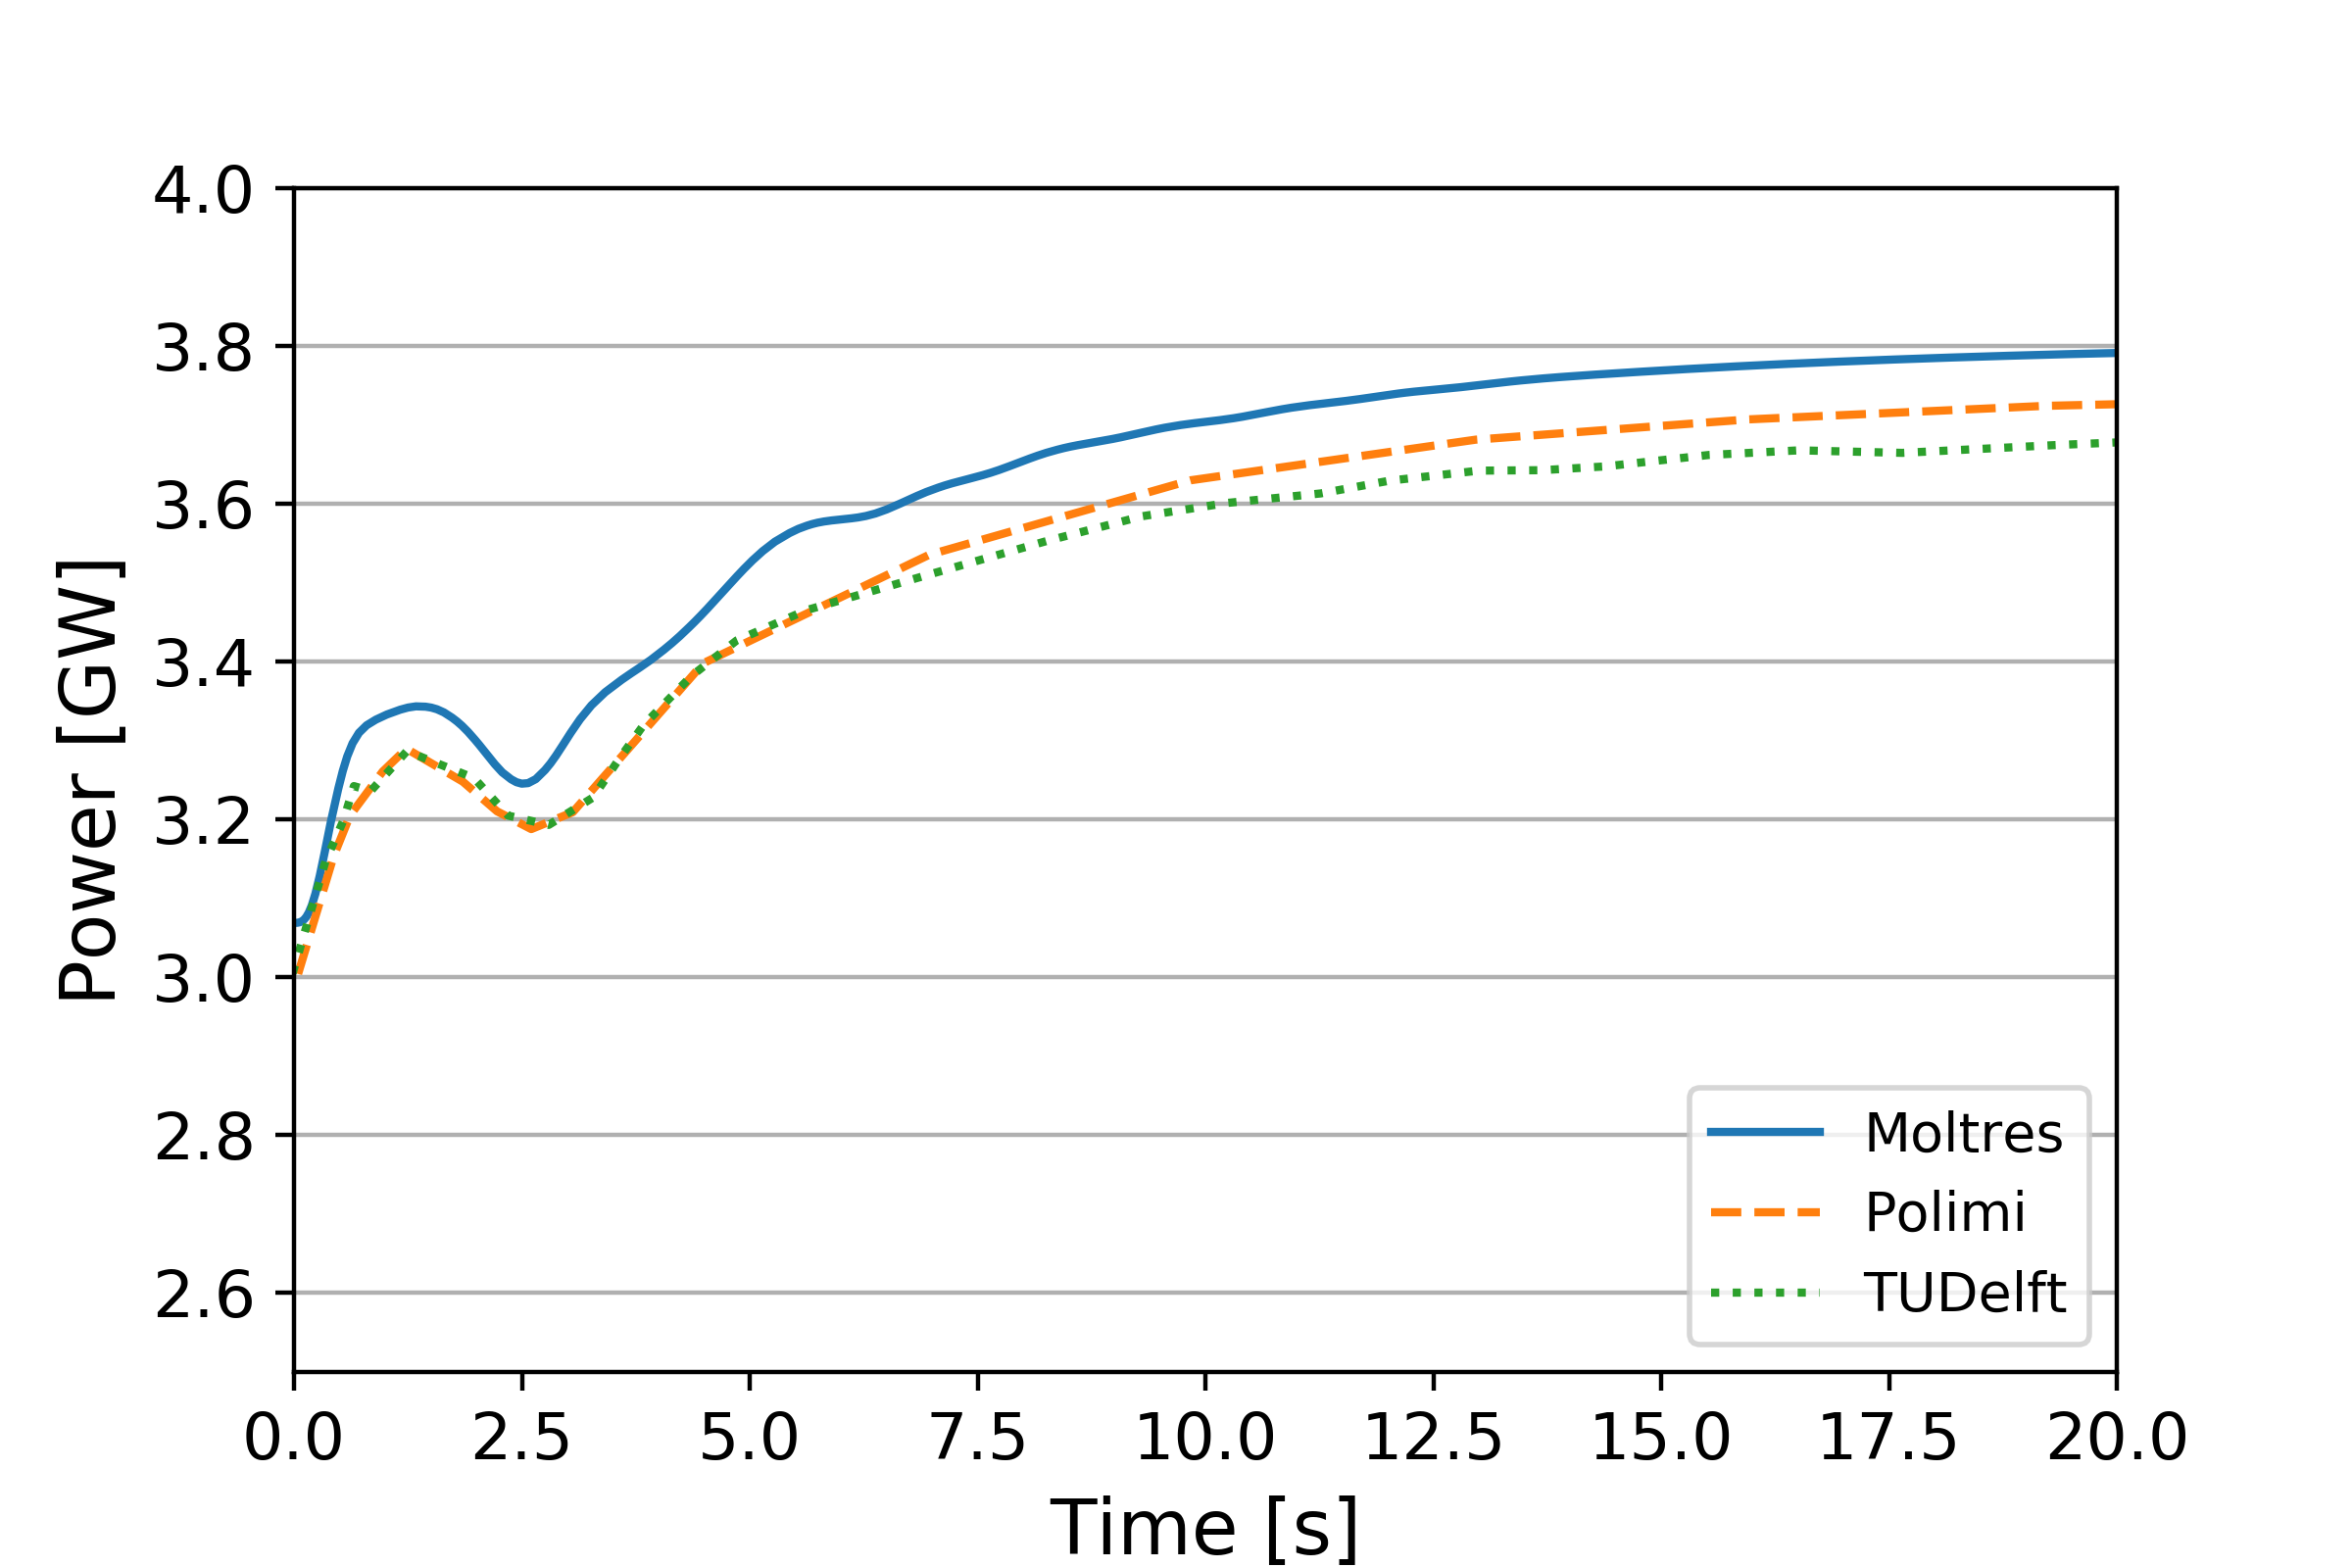
\includegraphics[width=\textwidth]{po-heat-short}
    \end{subfigure}
    \hfill
    \begin{subfigure}[t]{.485\textwidth}
        \centering
        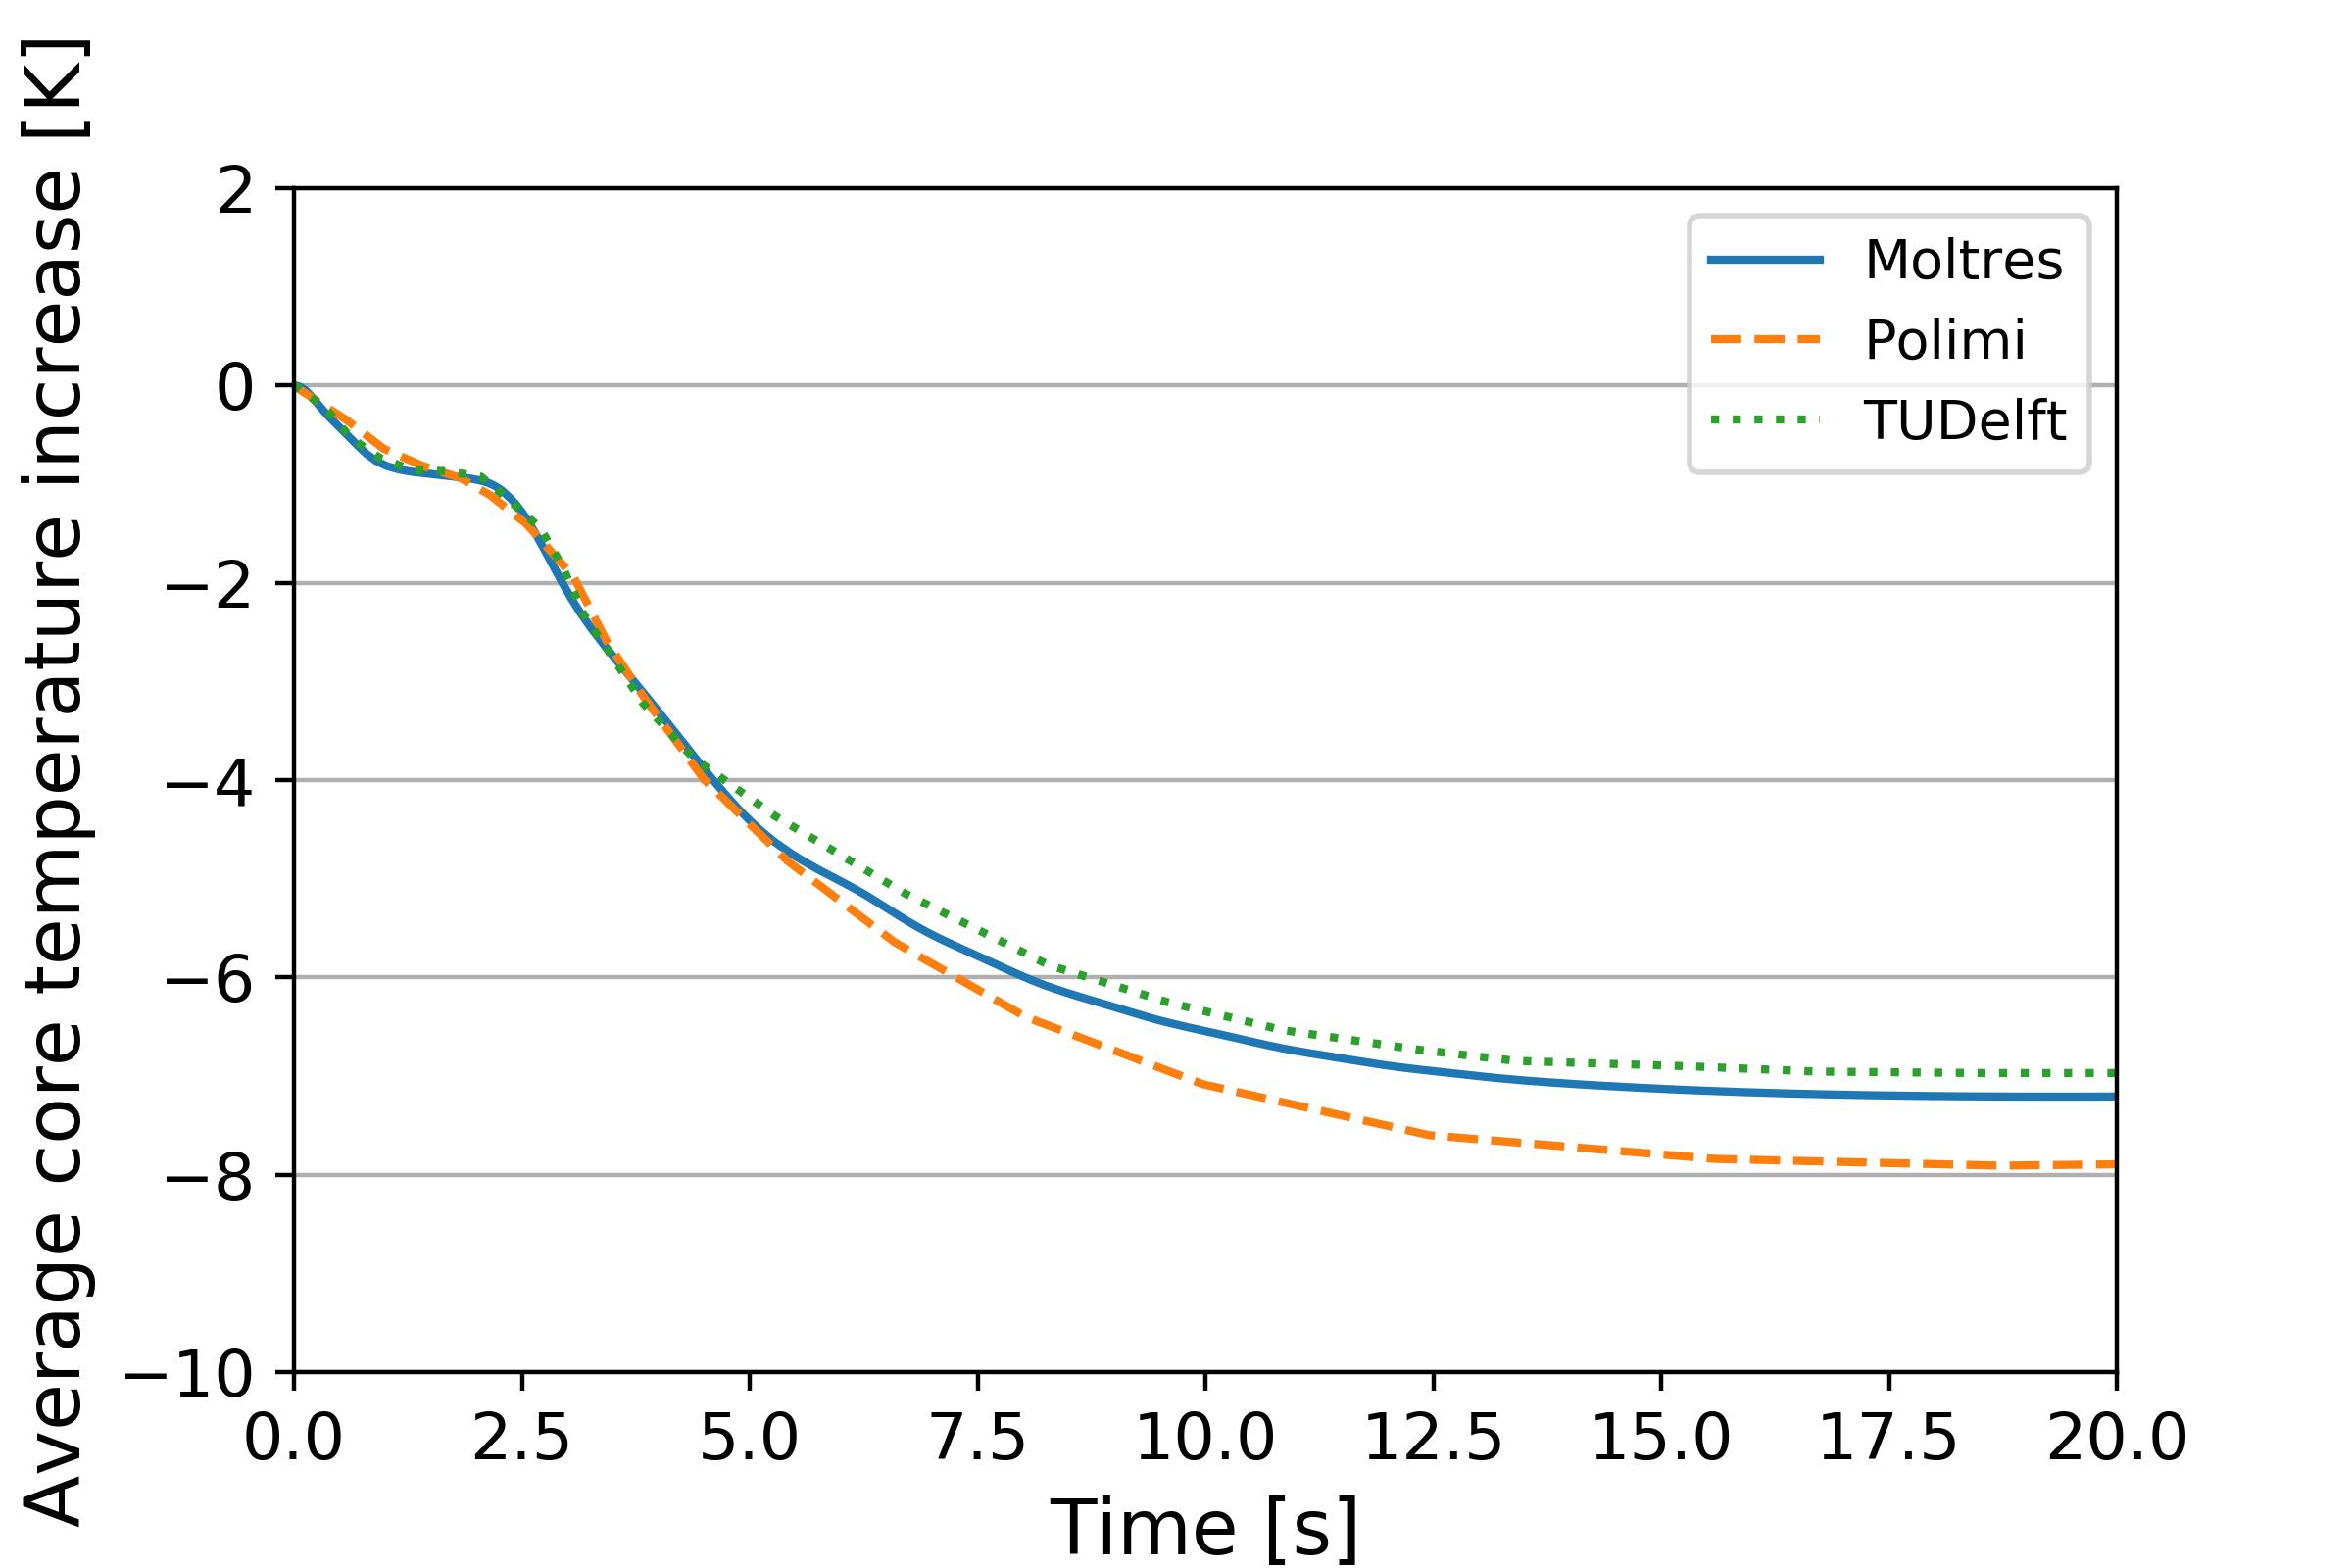
\includegraphics[width=\textwidth]{po-temp-short}
    \end{subfigure}
    \caption{Average core temperature increase during
    an unprotected pump overspeed transient in the Moltres, PoliMi, and
    TU Delft models \cite{fiorina_modelling_2014}.}
    \label{fig:poshort}
\end{figure}

\begin{figure}[htb!]
    \centering
    \begin{subfigure}[t]{.485\textwidth}
        \centering
        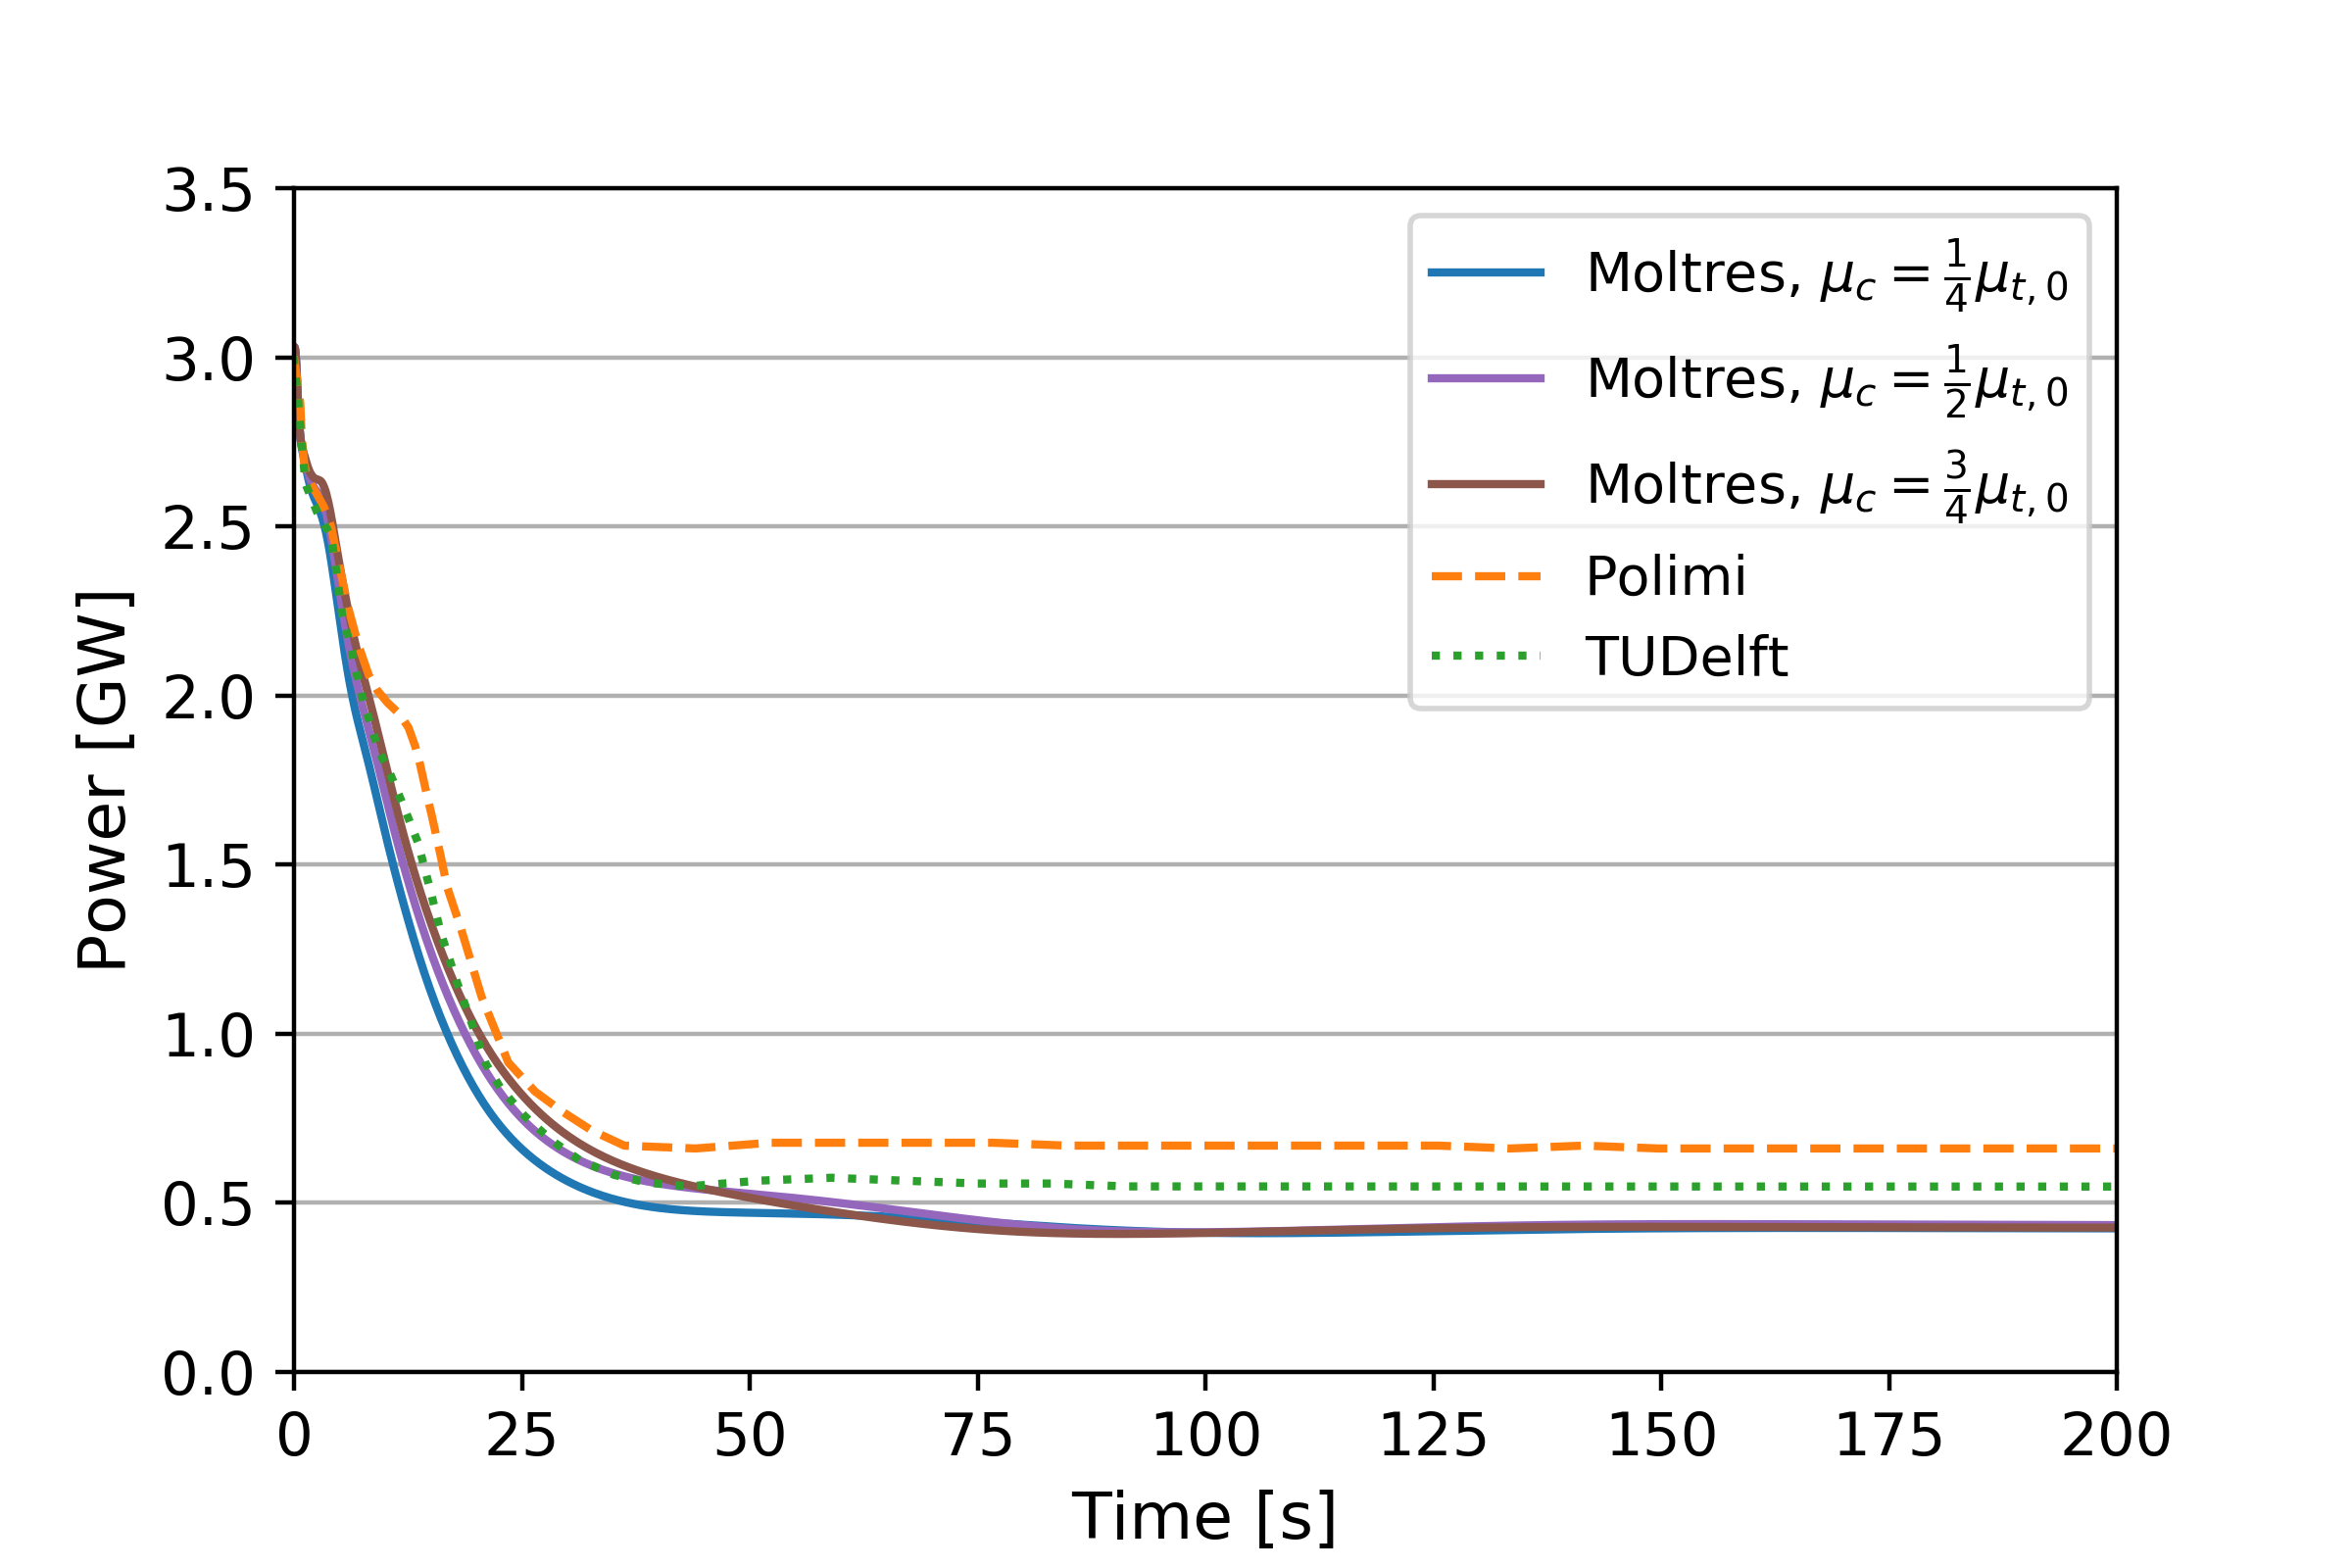
\includegraphics[width=\textwidth]{lof-heat}
    \end{subfigure}
    \hfill
    \begin{subfigure}[t]{.485\textwidth}
        \centering
        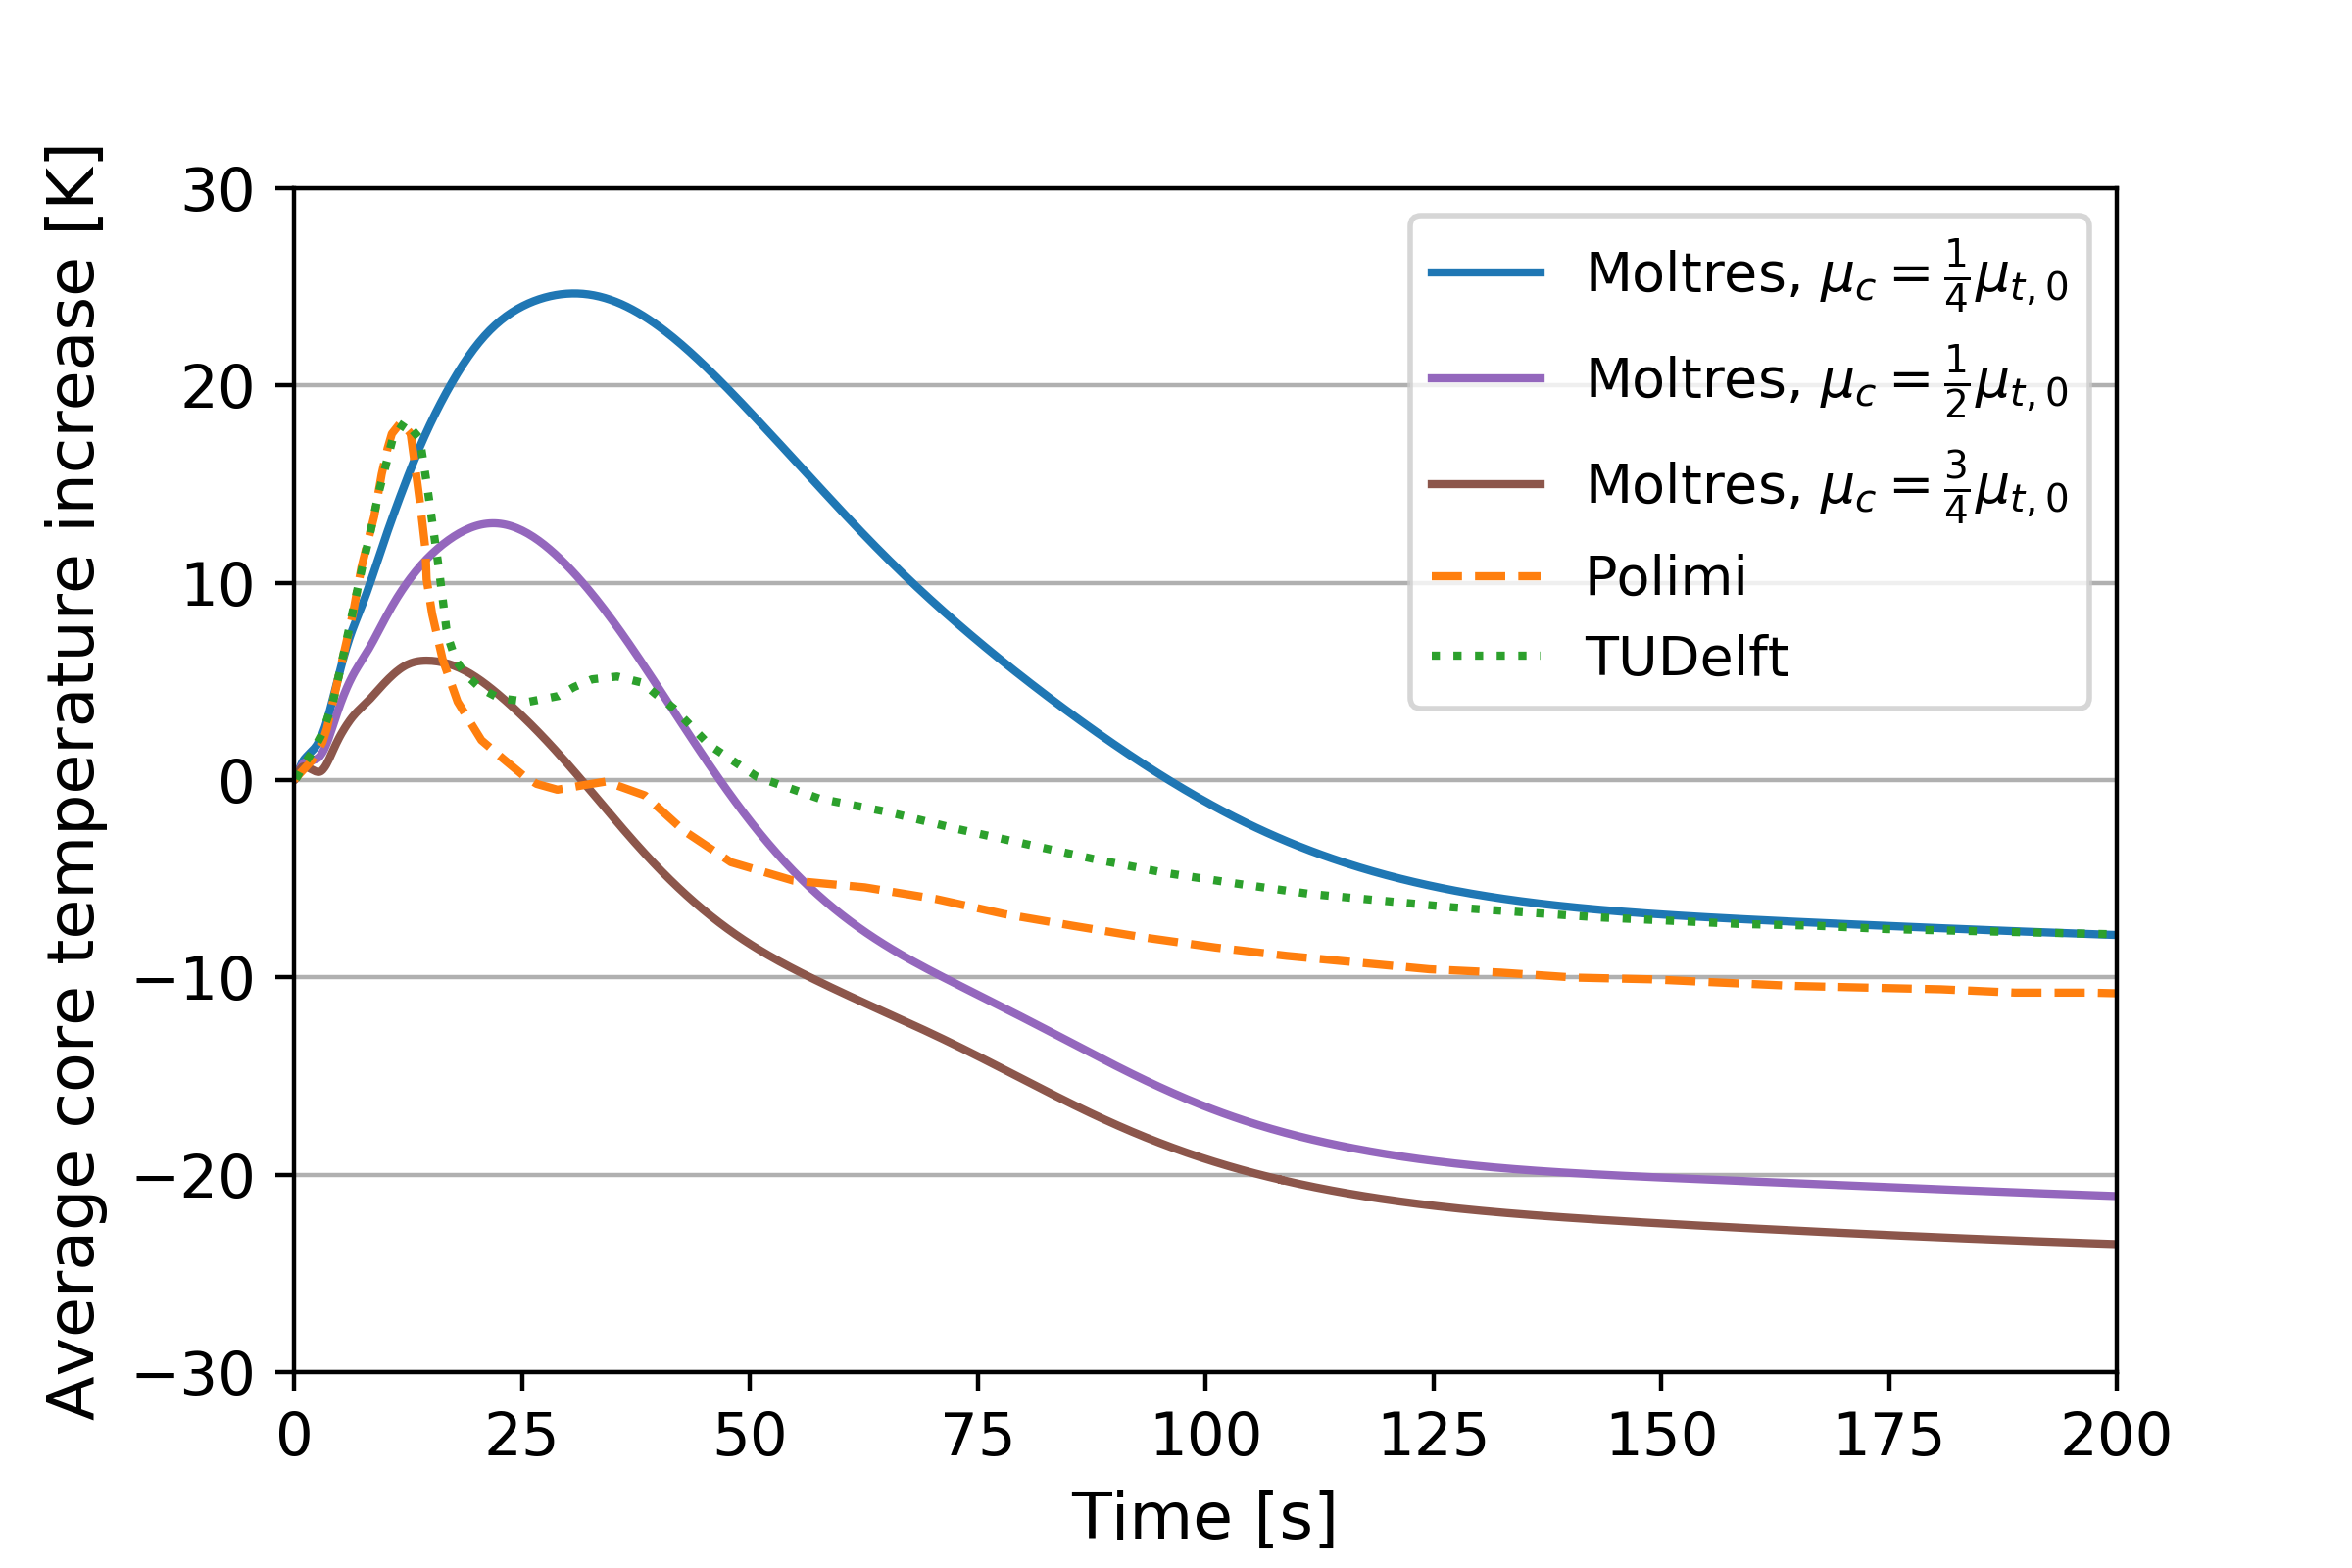
\includegraphics[width=\textwidth]{lof-temp}
    \end{subfigure}
    \caption{Power output and average core temperature increase during
    an unprotected loss of flow transient in the Moltres, PoliMi, and
    TU Delft models \cite{fiorina_modelling_2014}.}
    \label{fig:lof}
\end{figure}

\paragraph{Critical Assessment} \label{sec:msfr-critique}

Given the inherent and unique characteristics of \glspl{MSR}, the new
capabilities introduced in this work---coupling to incompressible Navier-Stokes
equations, precursor loop system, and decay heat model---are essential for
accurate \gls{MSR} modeling and simulation. This work demonstrated these
capabilities through steady-state and transient studies of a 2-D axisymmetric
\gls{MSFR} model similar to models by Fiorina et al.
\cite{fiorina_modelling_2014} and Aufiero et al.
\cite{aufiero_development_2014}. The Moltres model showed good agreement with
the other models in
most steady-state and transient cases with respect to the neutron flux, reactor
power, temperature, and velocity distributions. Most crucially, the
incompressible flow model reproduced characteristic regions of recirculating
flow and near-stagnant flow observed in the PoliMi and TU Delft \gls{MSFR}
models, which led to the formation of temperature hotspots and precursor
accumulation in the core.

However, significant discrepancies observed during pump-initiated transient
scenarios highlight the need for a proper turbulence model to capture
turbulent flow effects in some \gls{MSR} designs. Unlike the \gls{MSRE}, the
\gls{MSFR} experiences highly turbulent flow, whose Reynolds number is on the
order of $10^6$ under normal operating conditions. This level of turbulent flow
produces eddies of a wide range of length scales, and the computational demands
of the fine mesh and time resolution render it numerically unsolvable with
today's computational resources. Turbulence models allow for cheaper turbulence
simulations on coarser meshes by approximating the turbulent effects through
statistical analysis. Fiorina et al. \cite{fiorina_modelling_2014} employed the
$k$-$\epsilon$ turbulence model in their PoliMi and TU Delft models. Moltres
will benefit from coupling to similar intermediate-fidelity turbulence models
for turbulence simulations at reasonable computational costs.

While the Moltres model demonstrated good agreement with published data in the
steady-state, reactivity, and loss of heat sink scenarios, this work does not
thoroughly verify Moltres' capabilities for \gls{MSR} modeling.
The \gls{MSFR} simulations involve various physics models which combine to form
a complex multiphysics model. Therefore, it is difficult to pinpoint sources of
discrepancy with a high degree of certainty. Differences in the modeling
approaches also introduce discrepancies that cannot be reliably identified.
Moltres will benefit from code-to-code verification of
individual components responsible for modeling various physics present in
\glspl{MSR} and Moltres' multiphysics coupling approach.

\subsection{Objectives}
\begin{frame}
  \frametitle{Objectives}
  \begin{block}{\textbf{Overarching Goal of this Work}}
    Improve Moltres as a MSR simulation tool by enabling a wider range of MSR simulation
    scenarios.
  \end{block}
  \begin{block}{\textbf{Objectives}}
    \begin{enumerate}
      \item \textbf{Improve Multiphysics Capabilities in Moltres}
      \begin{itemize}
        \item Verify and validate existing multiphysics coupling capabilities in Moltres
        \item Implement a turbulence model in Moltres
      \end{itemize}
      \item \textbf{Develop a Hybrid Neutronics Method for Control Rod Modeling in Moltres}
      \begin{itemize}
        \item Develop and implement the hybrid $S_N$-diffusion method in Moltres
        \item Verify the hybrid method against high-fidelity neutronics codes and MSRE
          experimental data
        \item Demonstrate a time-dependent reactivity-initiated simulation using the hybrid
          method
      \end{itemize}
    \end{enumerate}
  \end{block}
\end{frame}


\section{Objective 1: Improve Multiphysics Coupling Capabilities}
\subsection{V\&V Study: MSRE Pump Start-up \& Coast-Down Transients}
\begin{frame}
  \frametitle{V\&V Study 2: MSRE Pump Start-up \& Coast-Down Transients}
  \textbf{Description of MSRE Pump Experiments}
  \begin{itemize}
    \item Starting from zero-power critical states with/without forced flow, the fuel salt pump
  was coasted down/started up
    \item Reactor was kept critical by a flux-servo controller moving the rod in response to flux
      changes
  \end{itemize}
  \begin{block}{\textbf{MSR Phenomena Involved}}
    \begin{itemize}
      \item DNP drift under time-varying flow
      \item Loss of delayed neutrons due to out-of-core DNP decay
    \end{itemize}
  \end{block}
  \begin{columns}
    \column{5.5cm}
    \begin{figure}
      \centering
      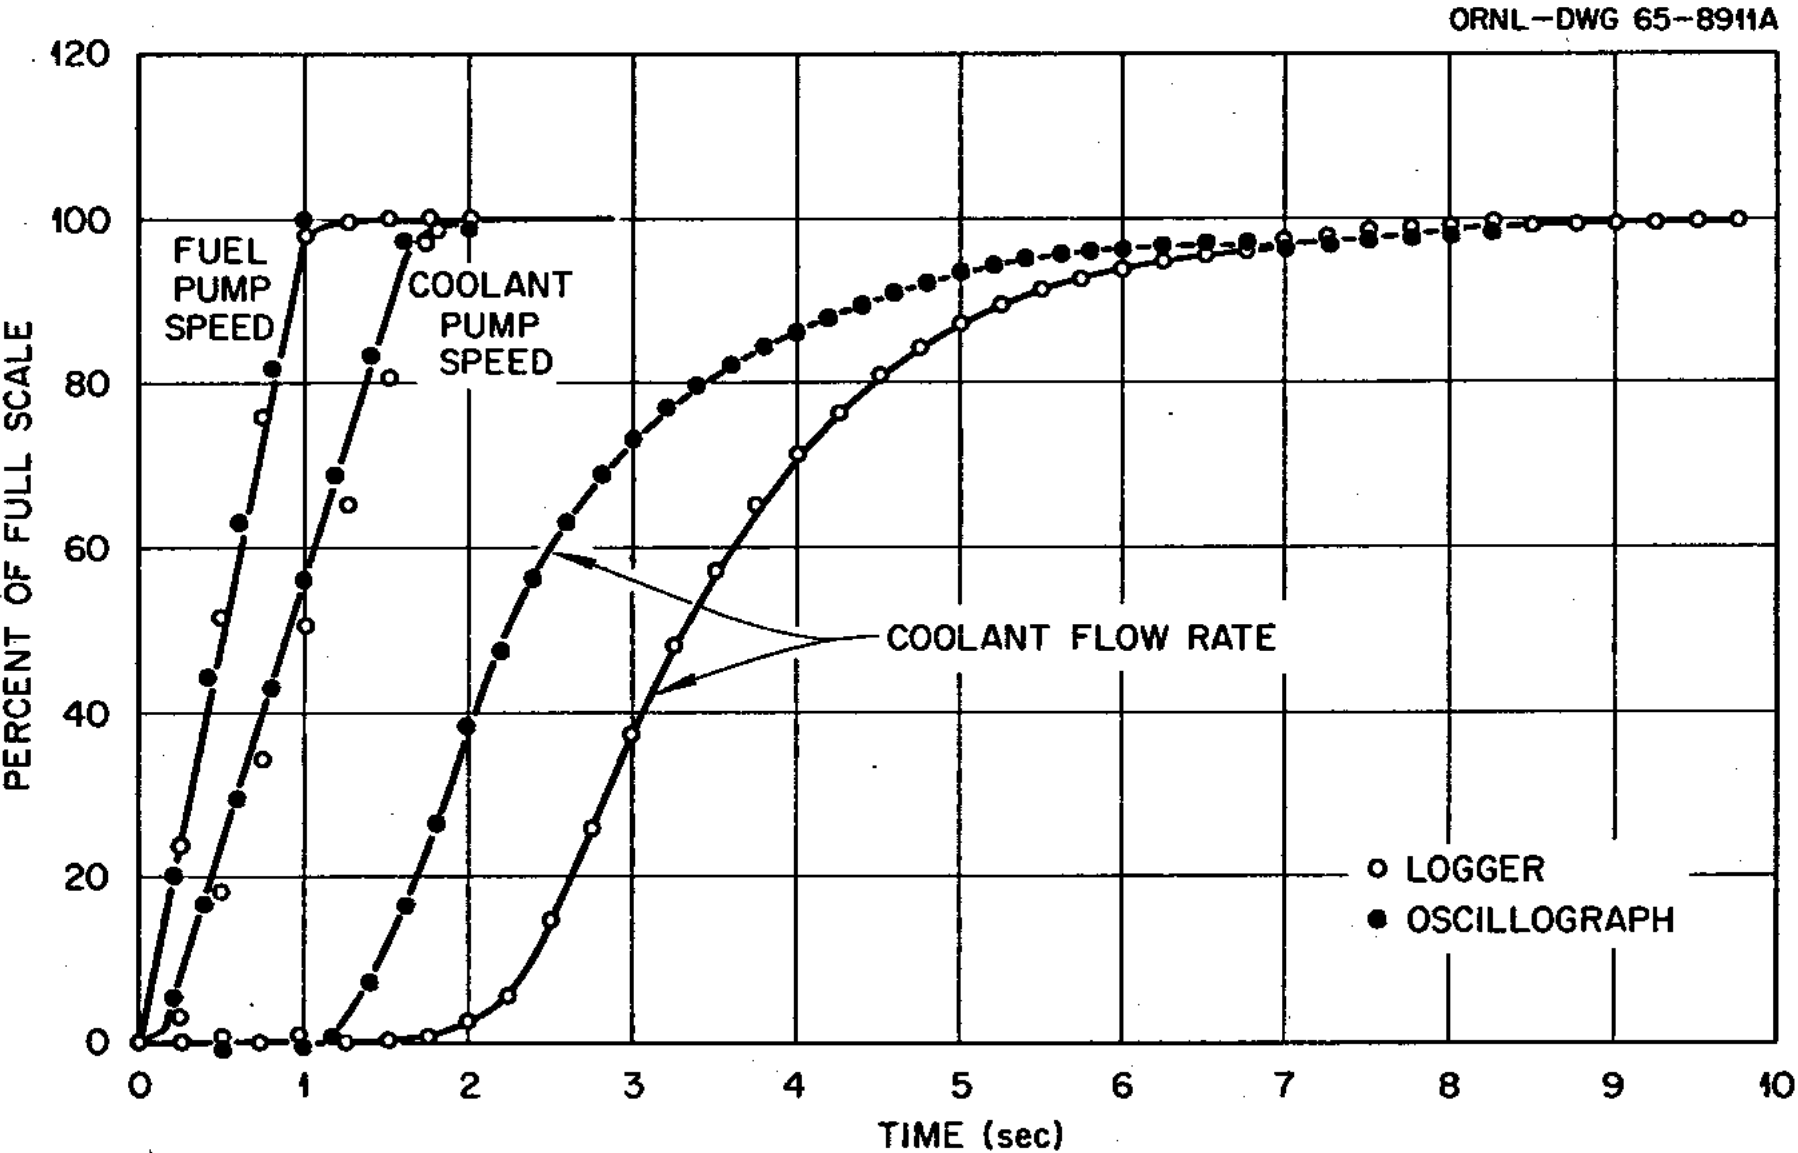
\includegraphics[width=.8\columnwidth]{images/msre-startup}
      \caption{MSRE start-up pump speed and flow rate experimental data
      \cite{prince_zero-power_1968}.}
    \end{figure}
    \column{5.5cm}
    \begin{figure}
      \centering
      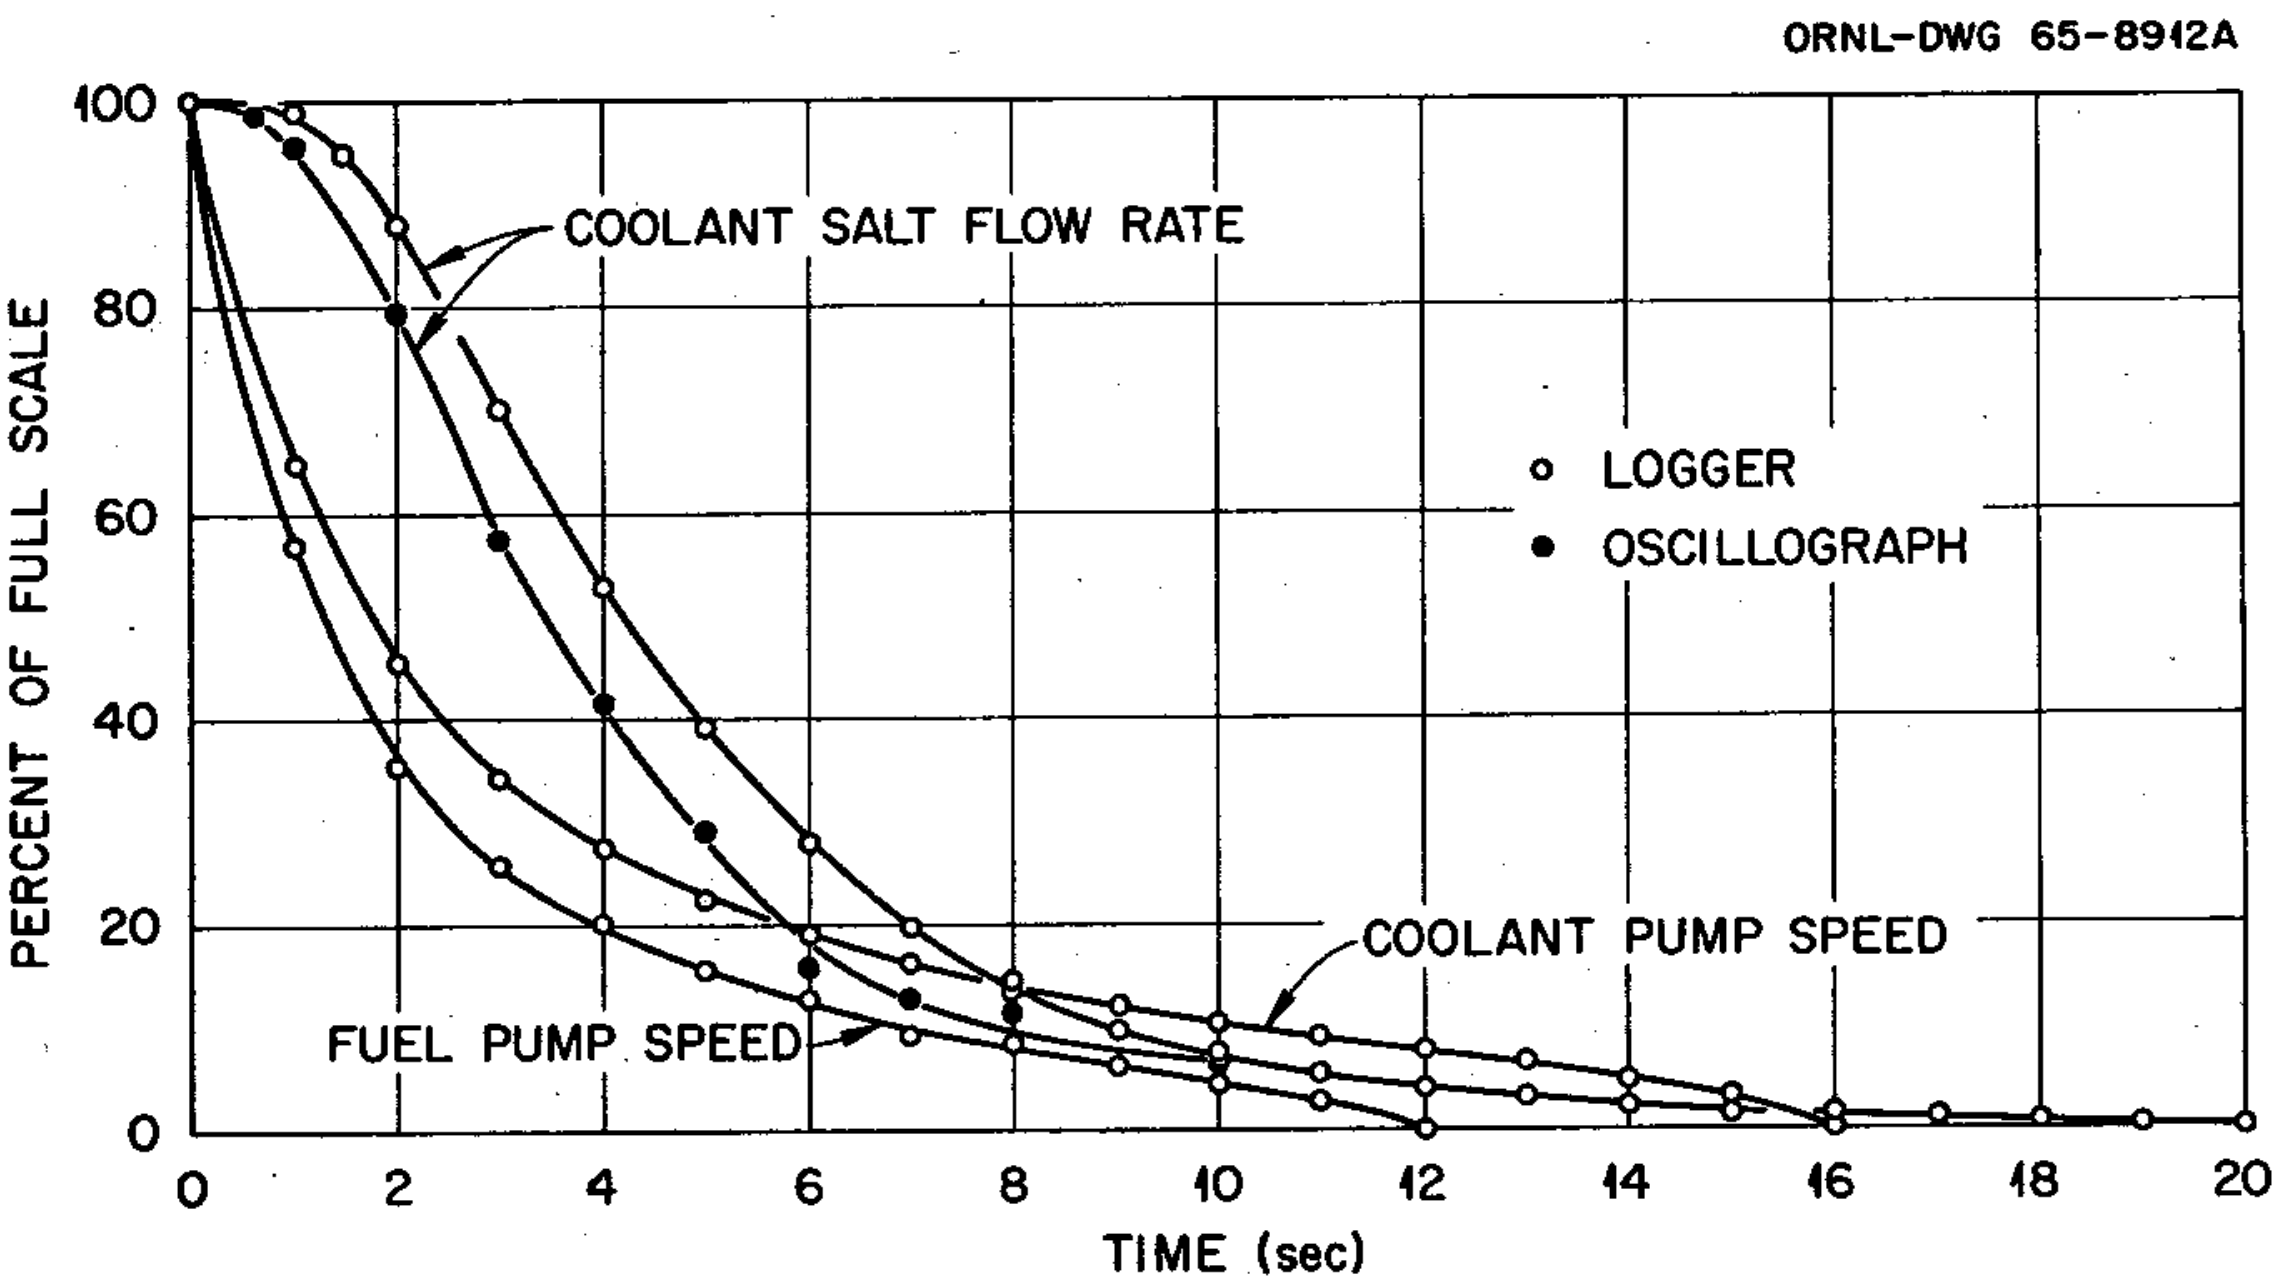
\includegraphics[width=.95\columnwidth]{images/msre-coastdown}
      \caption{MSRE coast-down pump speed and flow rate experimental data
      \cite{prince_zero-power_1968}.}
    \end{figure}
  \end{columns}
\end{frame}

%\begin{frame}
%  \frametitle{V\&V Study 2: MSRE Pump Start-up \& Coast-Down Transients}
%  \begin{block}{\textbf{MSR Phenomena Involved}}
%    \begin{itemize}
%      \item DNP drift under time-varying flow
%      \item Loss of delayed neutrons due to out-of-core DNP decay
%    \end{itemize}
%  \end{block}
%  \begin{block}{\textbf{Aim of the Study}}
%    Reproduce the reactivity curve of the control rod response with a 2-D axisymmetric model of the
%    MSRE in Moltres.
%  \end{block}
%  \begin{block}{\textbf{Study Objectives}}
%    \begin{itemize}
%      \item Develop a V\&V study based on the MSRE pump start-up \& coast-down
%        transients that is easily reproducible
%      \item Verify Moltres against QuasiMolto in collaboration with Aaron Reynolds
%        (formerly at Oregon State University)
%      \item Validate Moltres against MSRE experimental data for modeling \gls{DNP} drift
%    \end{itemize}
%  \end{block}
%\end{frame}

\begin{frame}
  \frametitle{V\&V Study 2: MSRE Pump Start-up \& Coast-Down Transients}
  \begin{columns}
    \column{6.5cm}
    \begin{block}{\textbf{Aim of the Study}}
      \begin{itemize}
         \item Develop a V\&V study based on the MSRE pump transients
         \item Verify Moltres against QuasiMolto in collaboration with Aaron Reynolds
           (formerly at Oregon State University)
         \item Validate Moltres against MSRE experimental data for modeling \gls{DNP} drift
       \end{itemize}
    \end{block}
    \begin{block}{\textbf{Modeling Approach}}
      \begin{itemize}
        \item Two neutron energy groups and six DNP groups
        \item Ignored upper and lower plena in the geometry
        \item Looped salt flow with a salt circulation time of 25.2 s
        \item $k$-eigenvalue calculation at every time-step ($dt=0.1$ s) in place of reactivity control
      \end{itemize}
    \end{block}
    \column{4.5cm}
    \begin{figure}[htb]
      \centering
      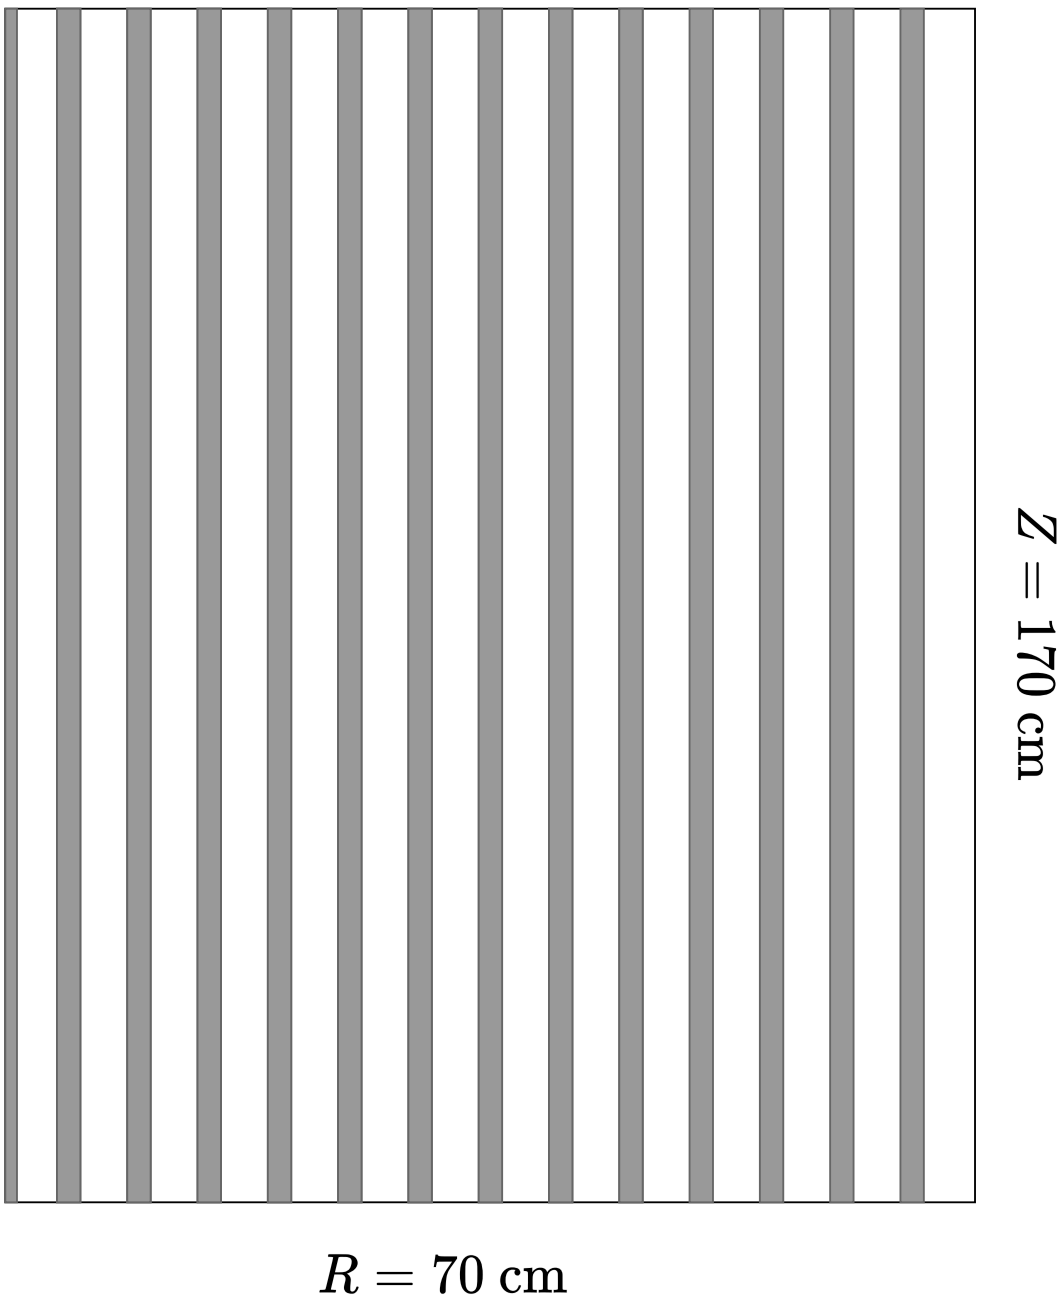
\includegraphics[width=0.8\columnwidth]{images/msre-2d}
      \caption{2-D axisymmetric model of the \gls{MSRE}.The gray and white regions represent fuel salt
      and graphite, respectively. Fuel salt channels are 1.25-cm wide and spaced at 5-cm intervals.}
      \label{fig:pump-geom}
    \end{figure}
  \end{columns}
\end{frame}

\begin{frame}
  \frametitle{V\&V Study 2: MSRE Pump Start-up \& Coast-Down Transients}
  \textbf{$k_\text{eff}$ Under Static \& Steady-Flow Conditions}
  \begin{table}[htb]
    \centering
    \caption{Multiplication factors $k_\text{eff}$ under static and steady salt flow conditions, and
    reactivity changes $\Delta\rho$ due to \gls{DNP} flow from the Moltres and QuasiMolto \gls{MSRE}
    models.}
    \begin{tabular}{l S S S}
      \toprule
      \multirow{2}{*}{Code} & \multicolumn{2}{c}{$k_\text{eff}$} & {$\Delta\rho$ due to} \\
                            & {Static} & {Steady flow} & {\gls{DNP} flow} \\
                            \cmidrule(r){1-1} \cmidrule(rl){2-3} \cmidrule(l){4-4}
      Moltres & 1.05625 & 1.05311 & -282.4 \\
      QuasiMolto & 1.05603 & 1.05290 & -281.7 \\
      \bottomrule
    \end{tabular}
    \label{table:msre-pump-keff}
  \end{table}
  \begin{itemize}
    \item Excellent agreement between Moltres and QuasiMolto under static and steady-flow conditions prior
  to the pump transients.
  \end{itemize}
\end{frame}

\begin{frame}
  \frametitle{V\&V Study 2: MSRE Pump Start-up \& Coast-Down Transients}
  \textbf{Neutron Flux Distributions Under Static Conditions}
  \begin{figure}[h]
    \centering
    \begin{subfigure}[b]{0.48\columnwidth}
      \centering
      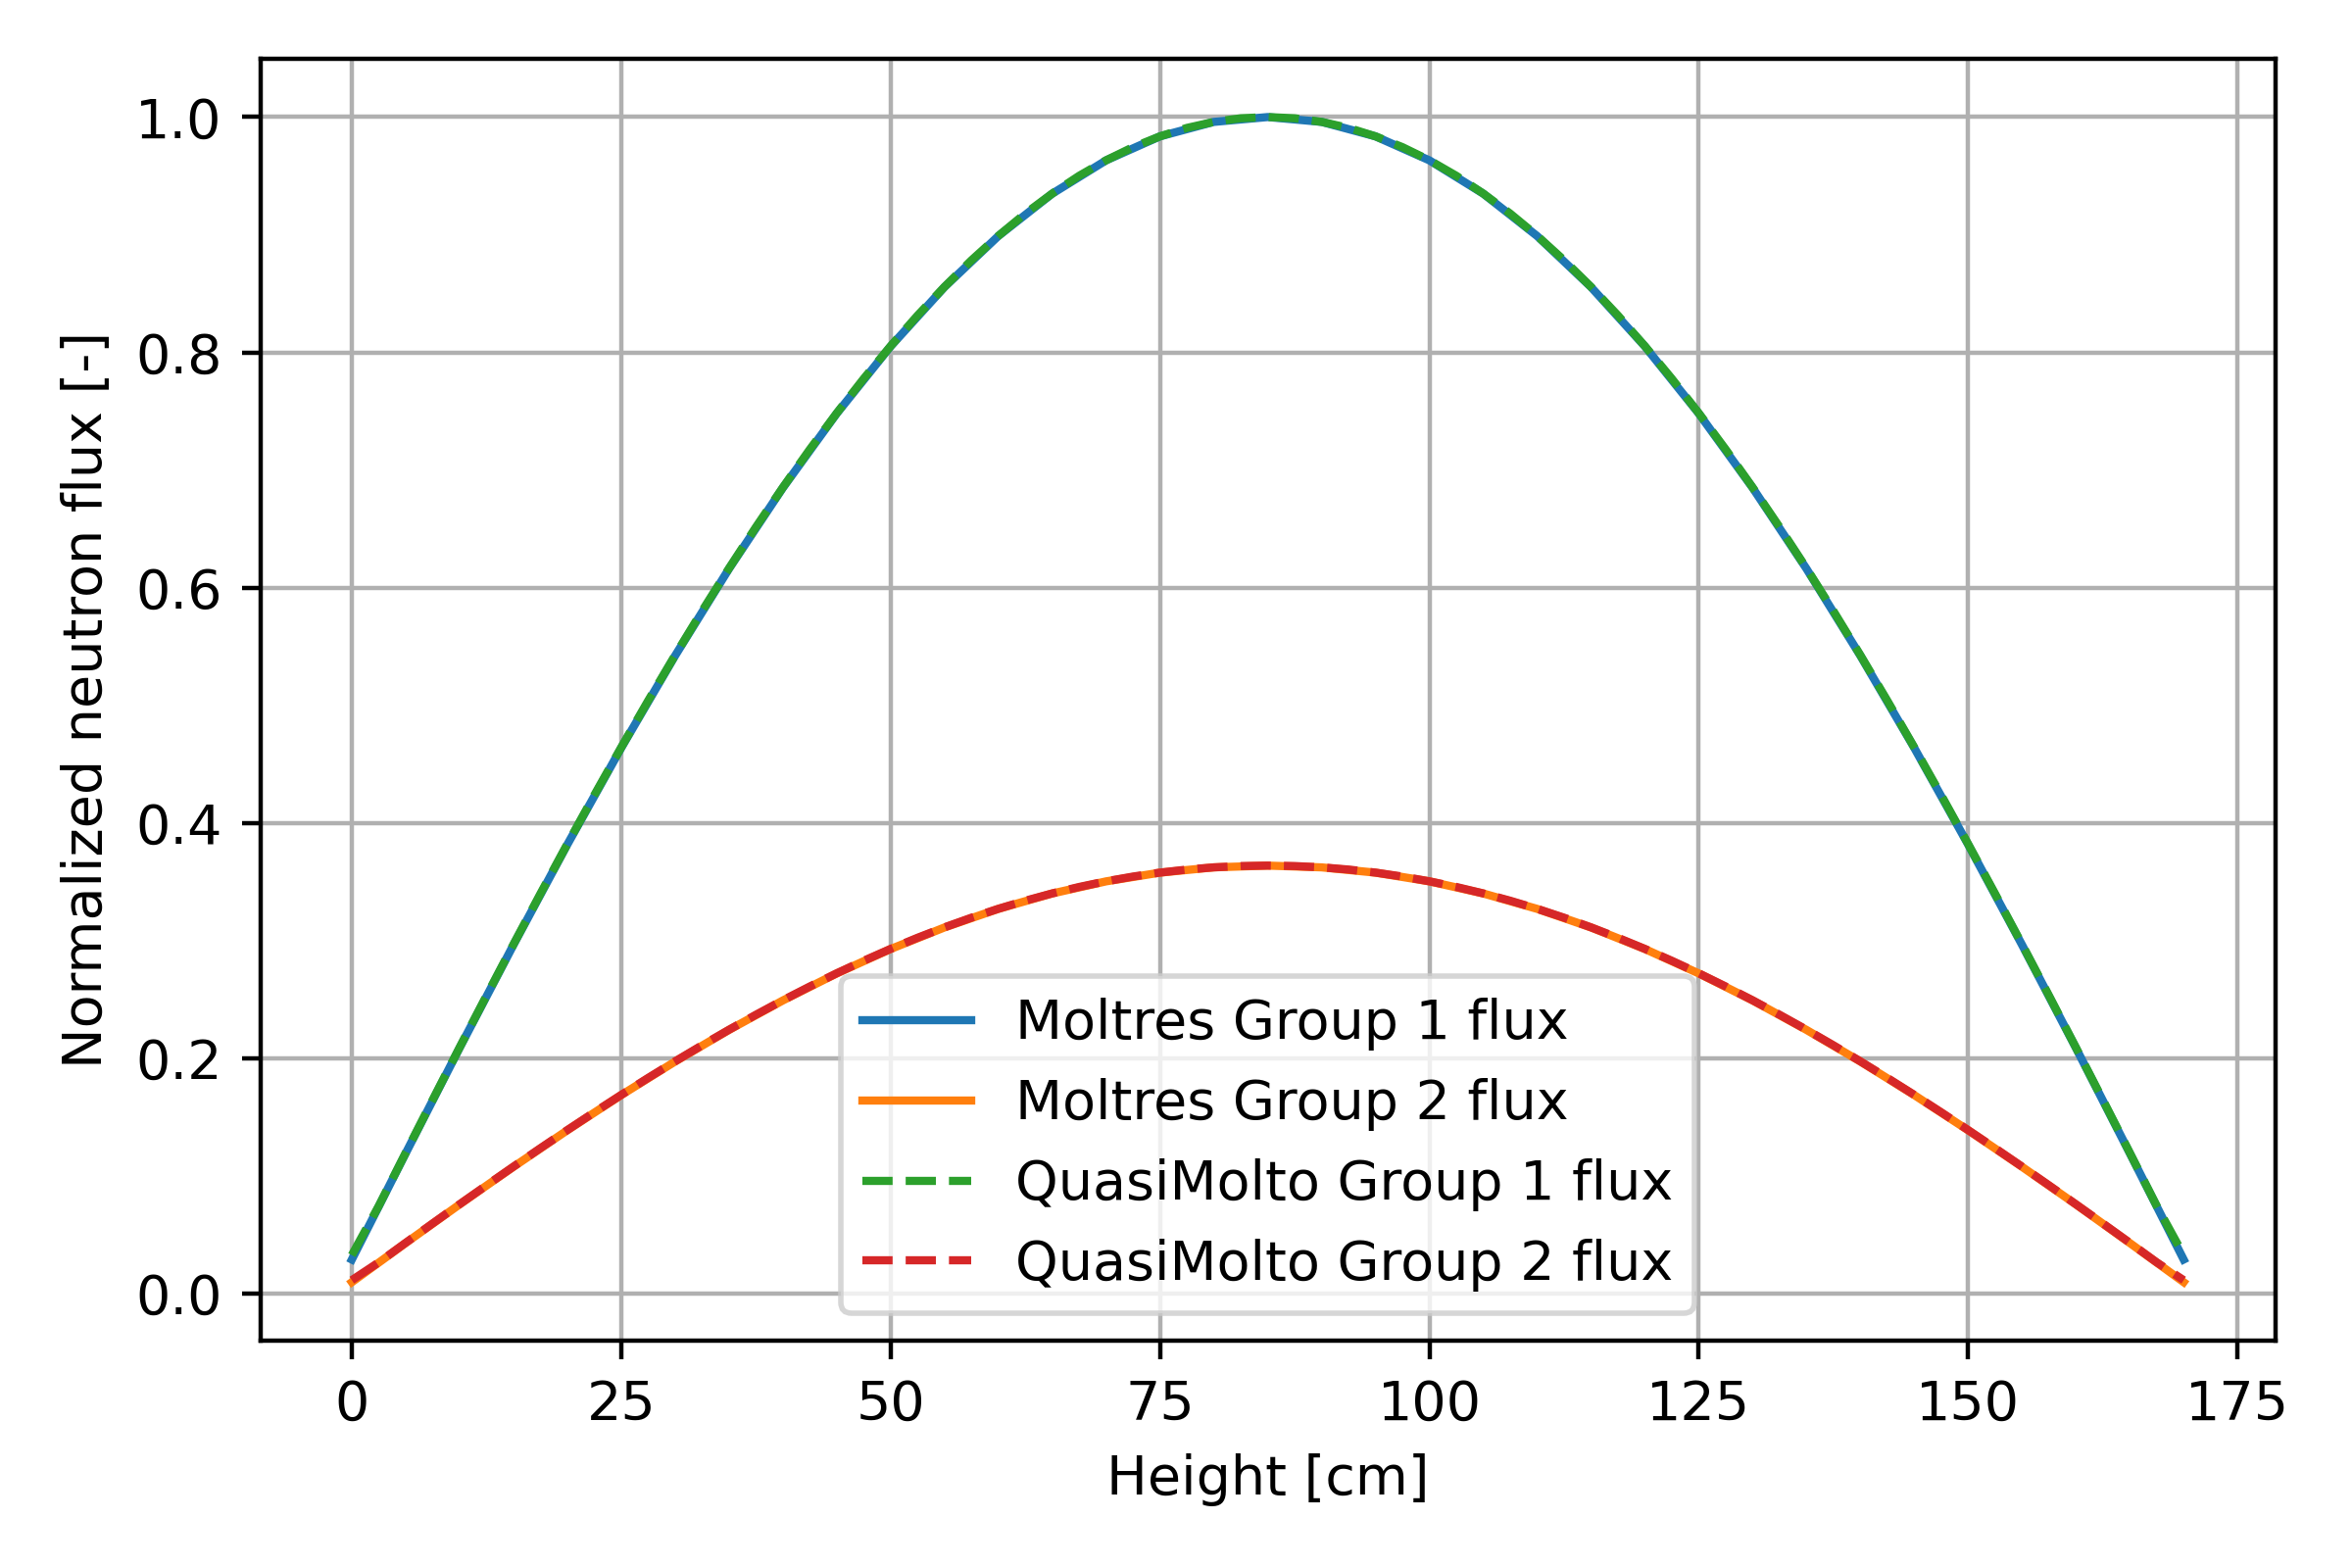
\includegraphics[width=\columnwidth]{centerline_flux}
      \caption{Normalized centerline neutron fluxes.}
      \label{fig:centerline-flux-dist}
    \end{subfigure}
    \hfill
    \begin{subfigure}[b]{0.48\columnwidth}
      \centering
      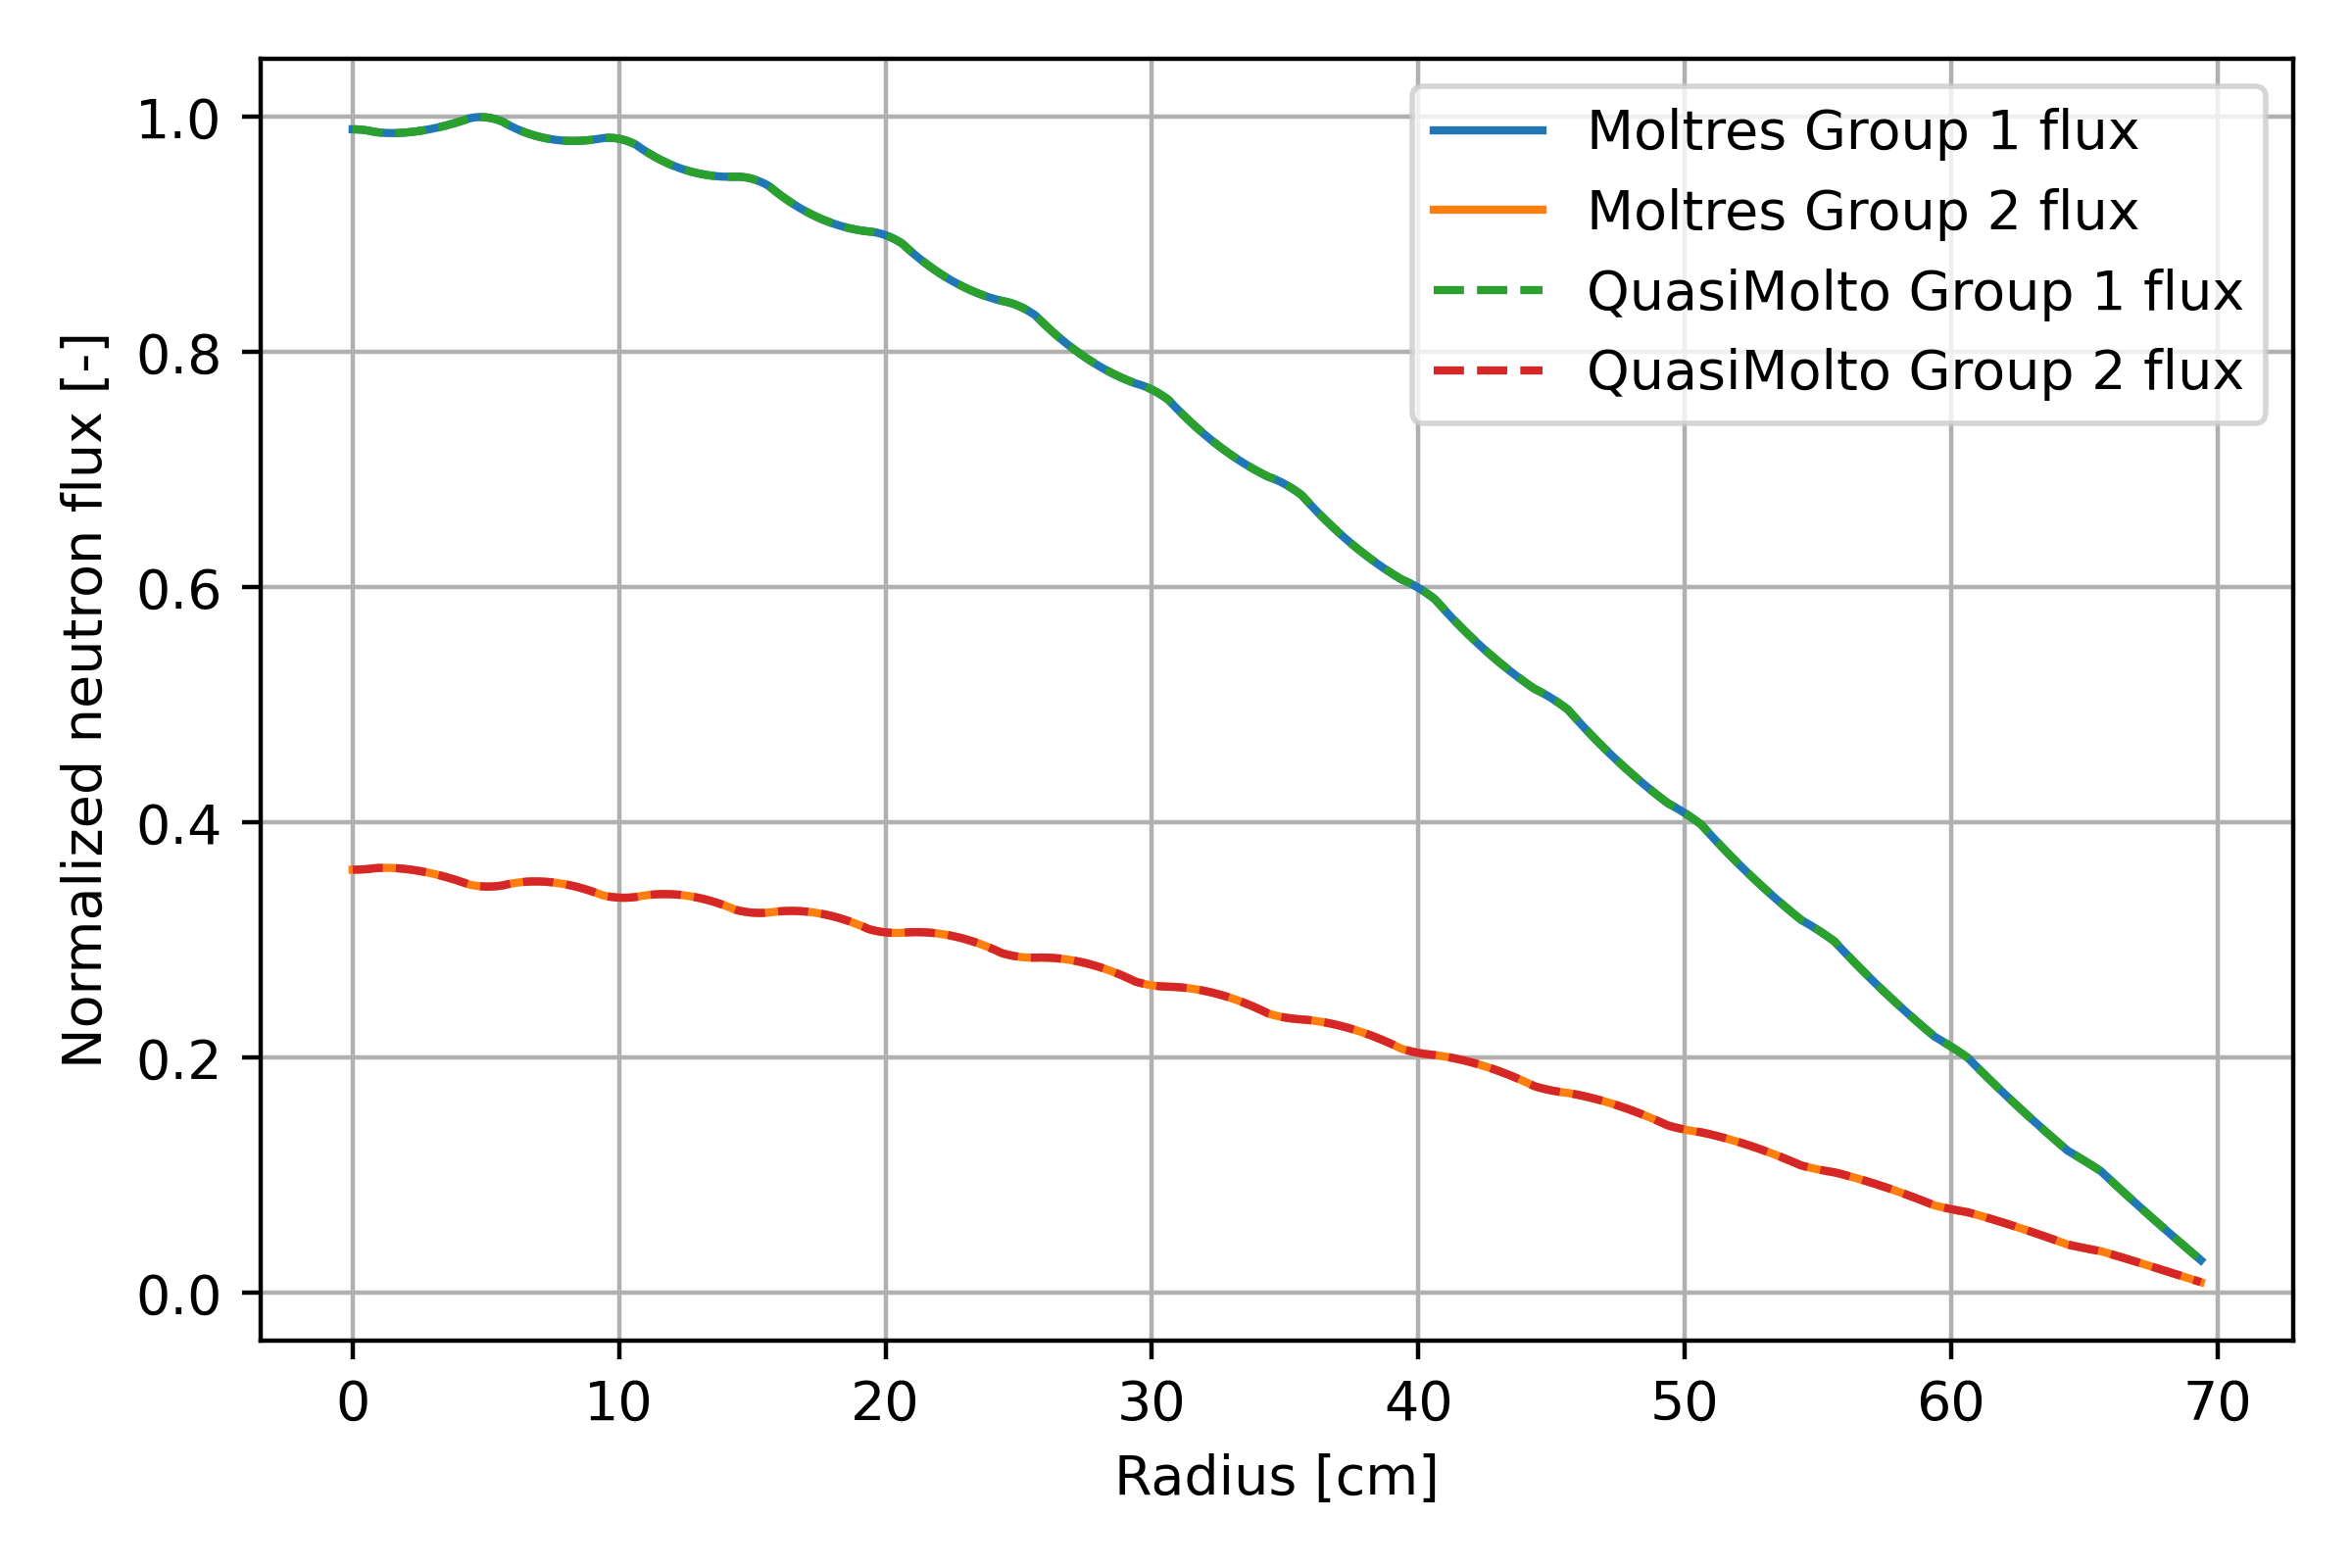
\includegraphics[width=\columnwidth]{midplane_flux}
      \caption{Normalized midplane neutron fluxes.}
      \label{fig:midplane-flux-dist}
    \end{subfigure}
    \caption{Neutron flux distributions comparing QuasiMolto and Moltres
    \gls{MSRE} models under static conditions. Maximum relative difference $\approx 0.8 \%$.}
    \label{fig:centerline-flux}
  \end{figure}
  \begin{itemize}
    \item Perfect overlap in centerline and midplane neutron fluxes between Moltres and QuasiMolto.
  \end{itemize}
\end{frame}

\begin{frame}
  \frametitle{V\&V Study 2: MSRE Pump Start-up \& Coast-Down Transients}
  \textbf{DNP Distributions Under Static Conditions}
  \begin{figure}[t]
    \centering
    \begin{subfigure}[b]{0.48\columnwidth}
      \centering
      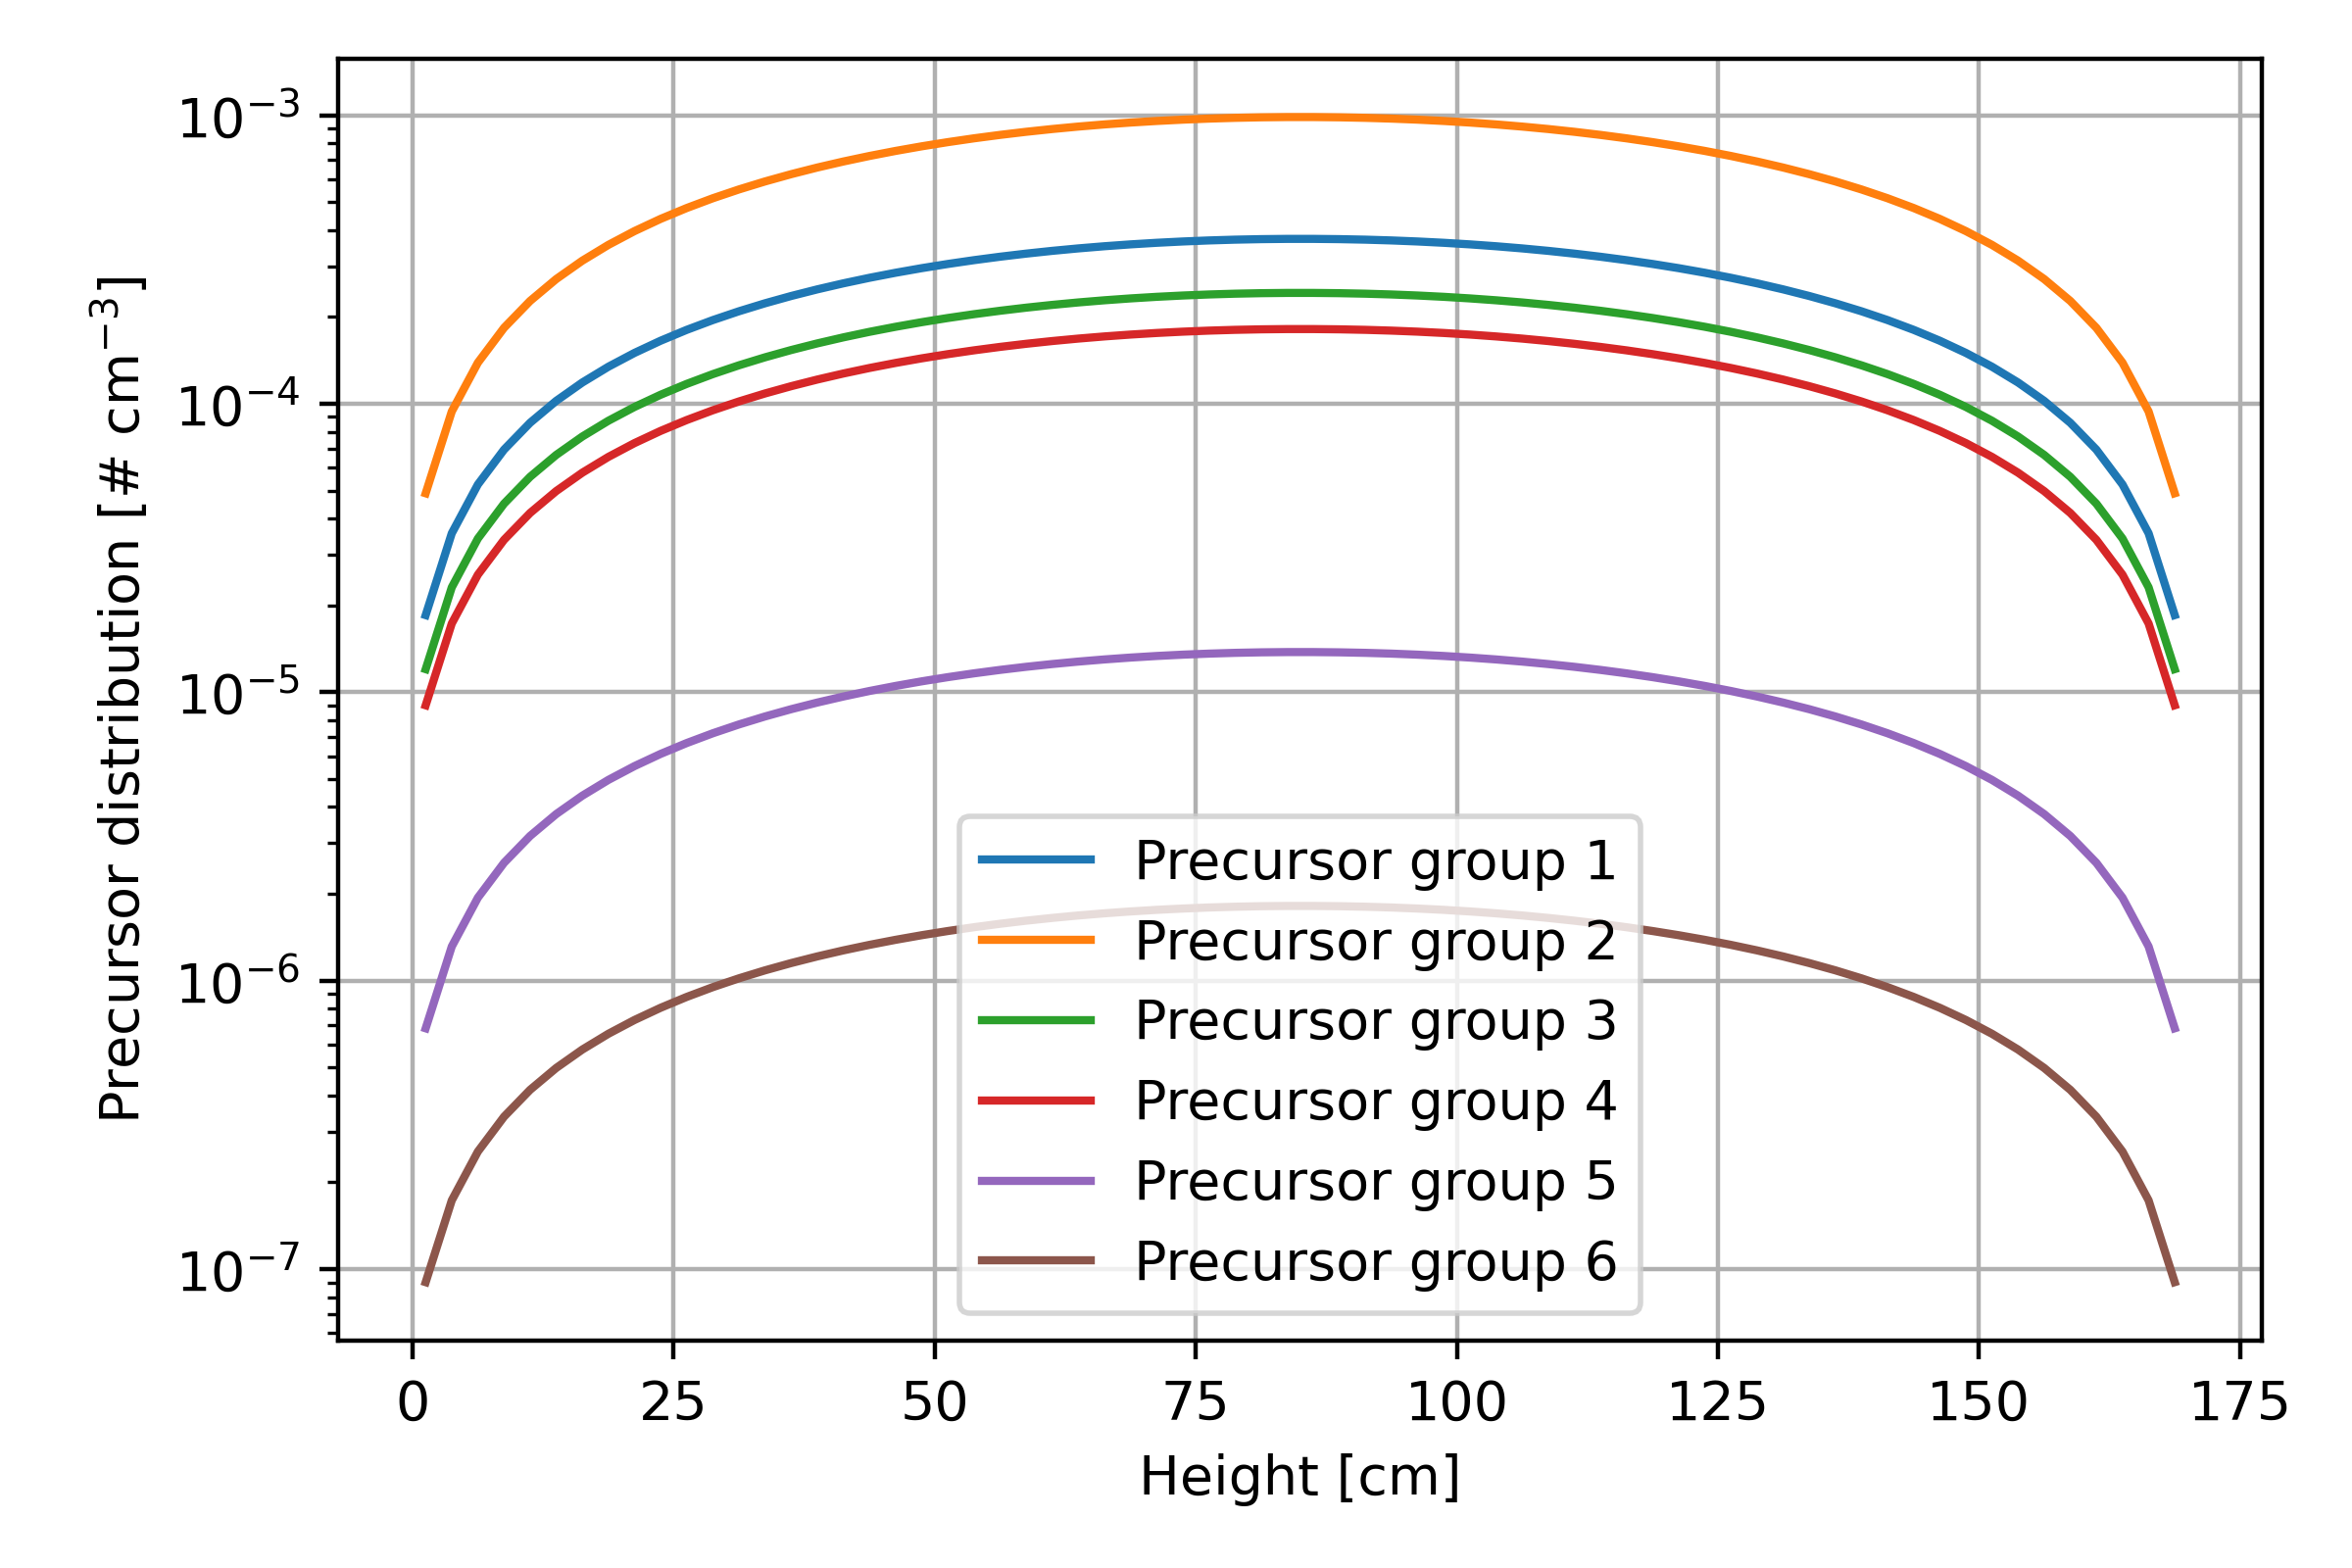
\includegraphics[width=\columnwidth]{centerline_pre}
      \caption{Normalized centerline \gls{DNP} distributions.}
      \label{fig:centerline-pre-dist}
    \end{subfigure}
    \hfill
    \begin{subfigure}[b]{0.48\columnwidth}
      \centering
      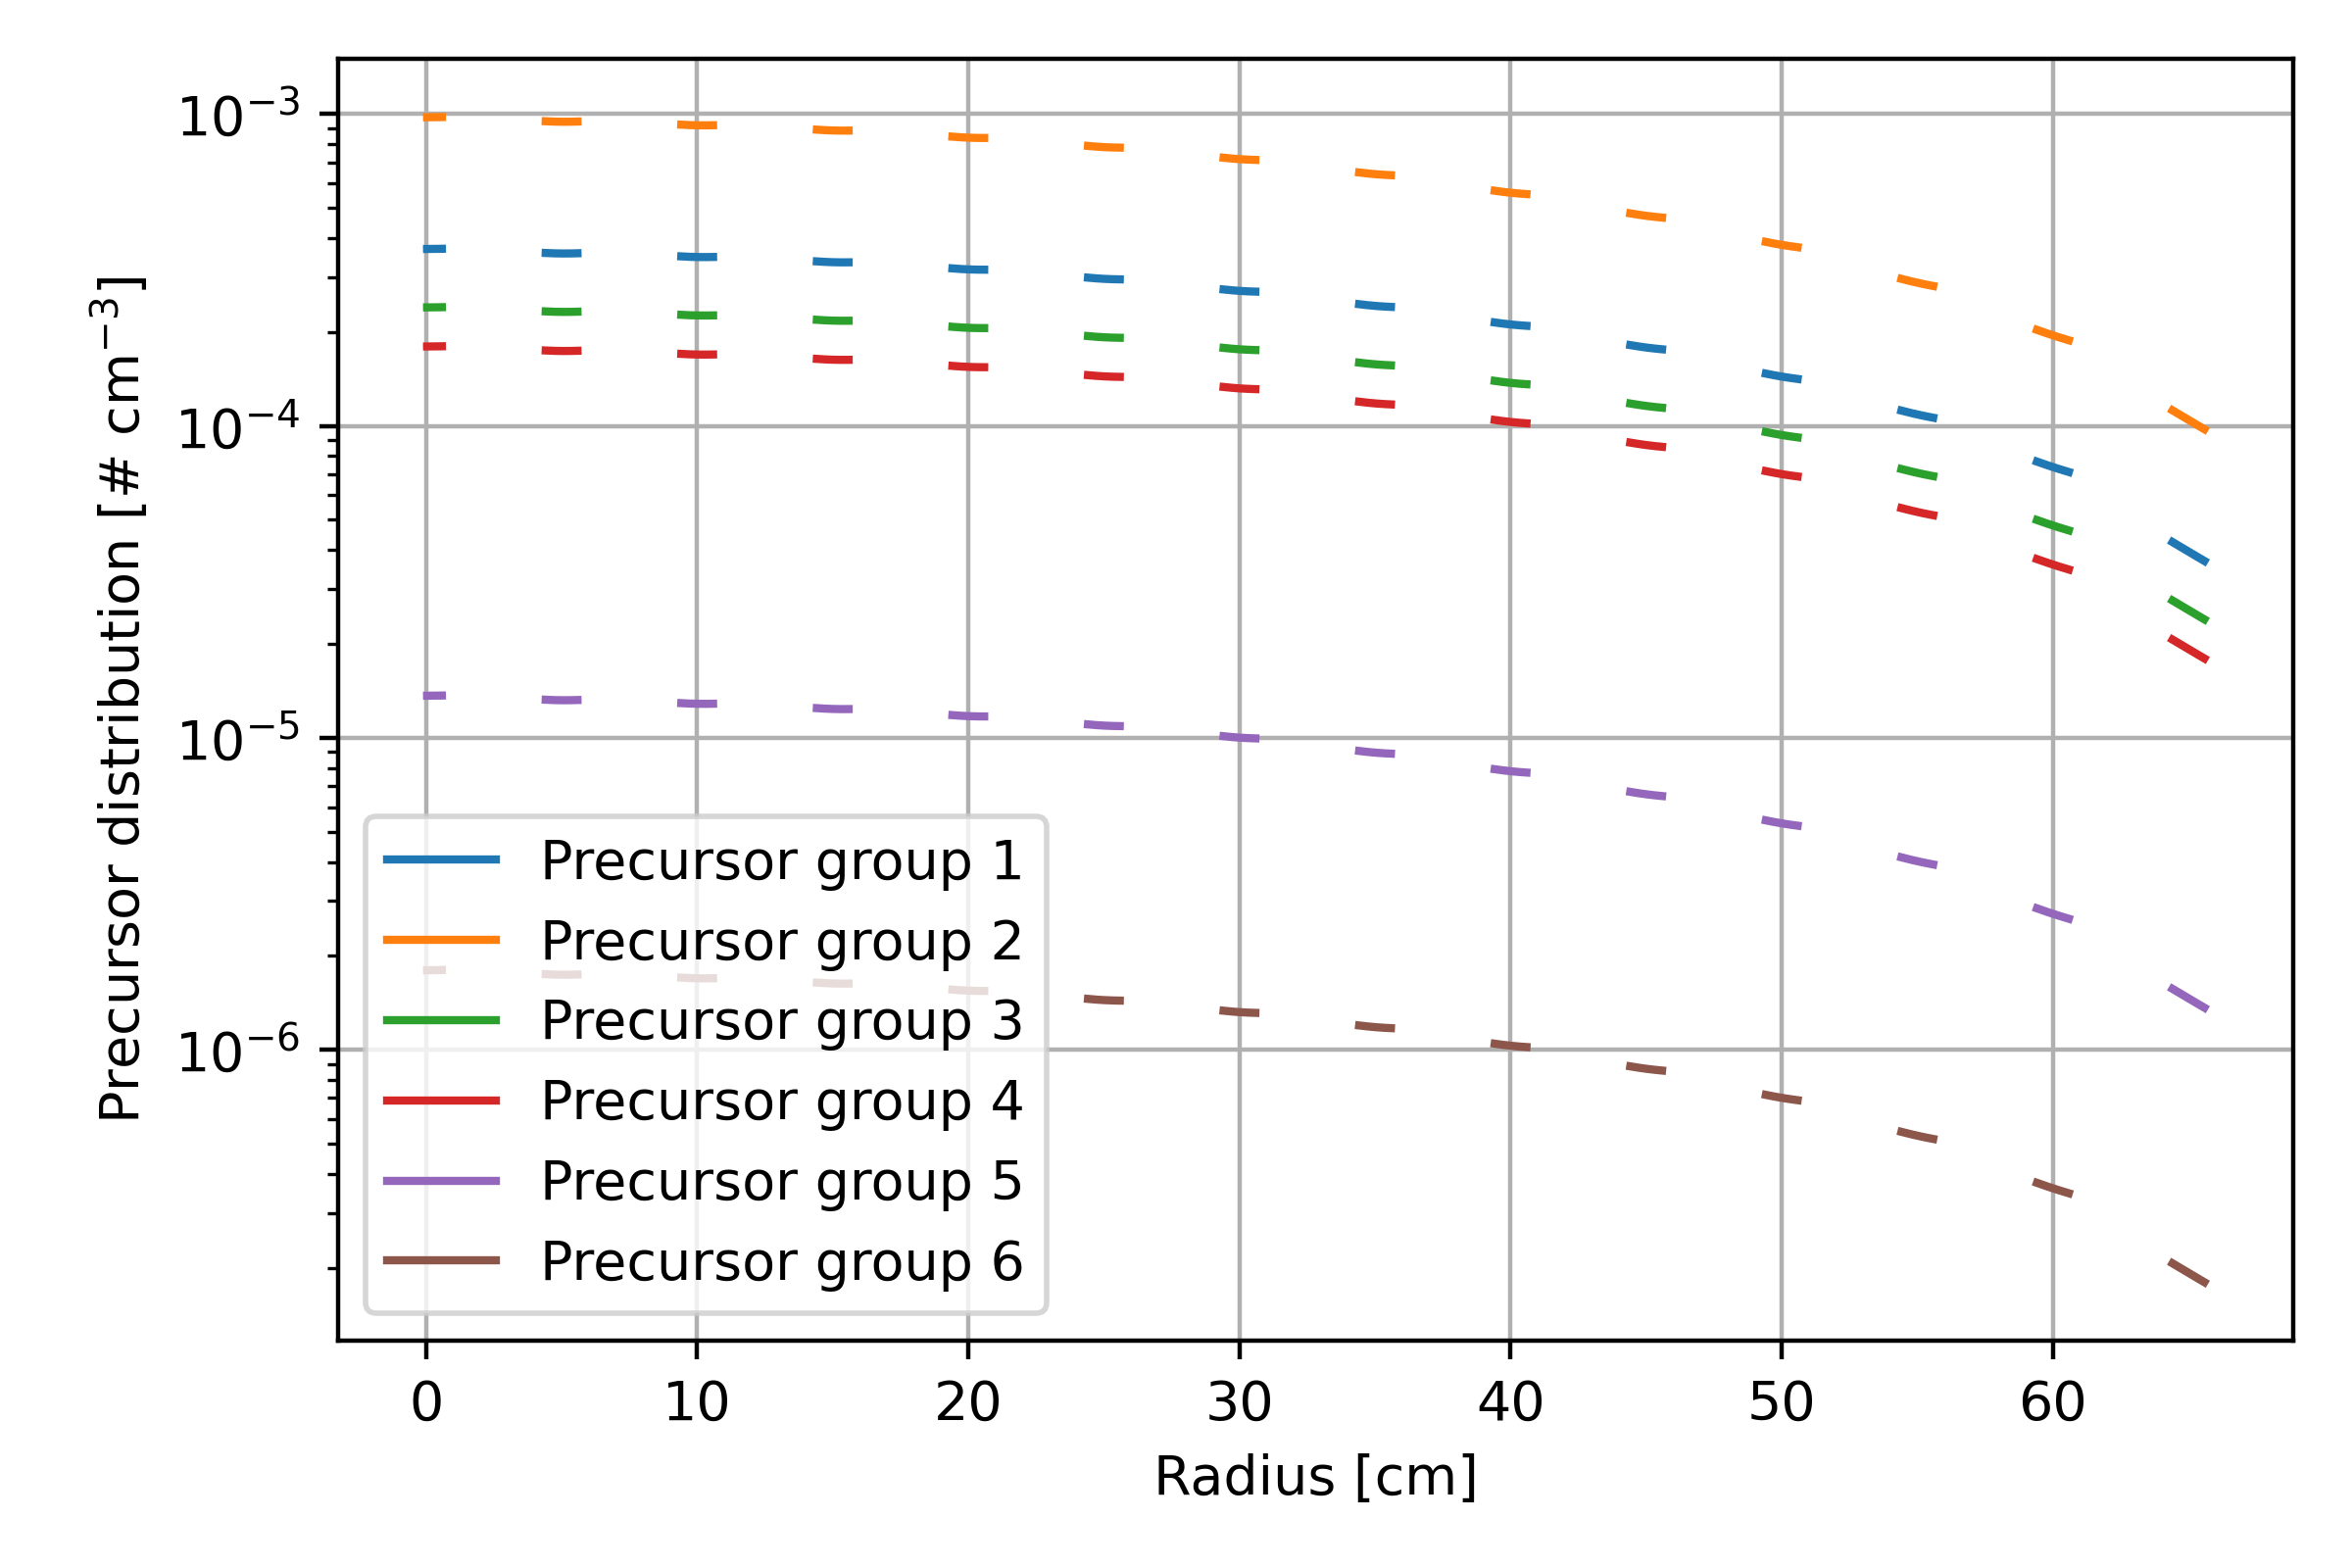
\includegraphics[width=\columnwidth]{midplane_pre}
      \caption{Normalized midplane \gls{DNP} distributions.}
      \label{fig:midplane-pre-dist}
    \end{subfigure}
    \caption{\gls{DNP} distribution from Moltres and ratios comparing QuasiMolto and
    Moltres models under static \gls{MSRE} conditions. Maximum relative difference $\approx 0.1 \%$.}
    \label{fig:centerline-pre}
  \end{figure}
  \begin{itemize}
    \item Perfect overlap in centerline and midplane DNP distributions between Moltres and QuasiMolto.
  \end{itemize}
\end{frame}

\begin{frame}
  \frametitle{V\&V Study 2: MSRE Pump Start-up \& Coast-Down Transients}
  \textbf{Pump Start-Up Transient Results}
  \begin{columns}
  \column{5.5cm}
  \begin{figure}[t]
    \centering
    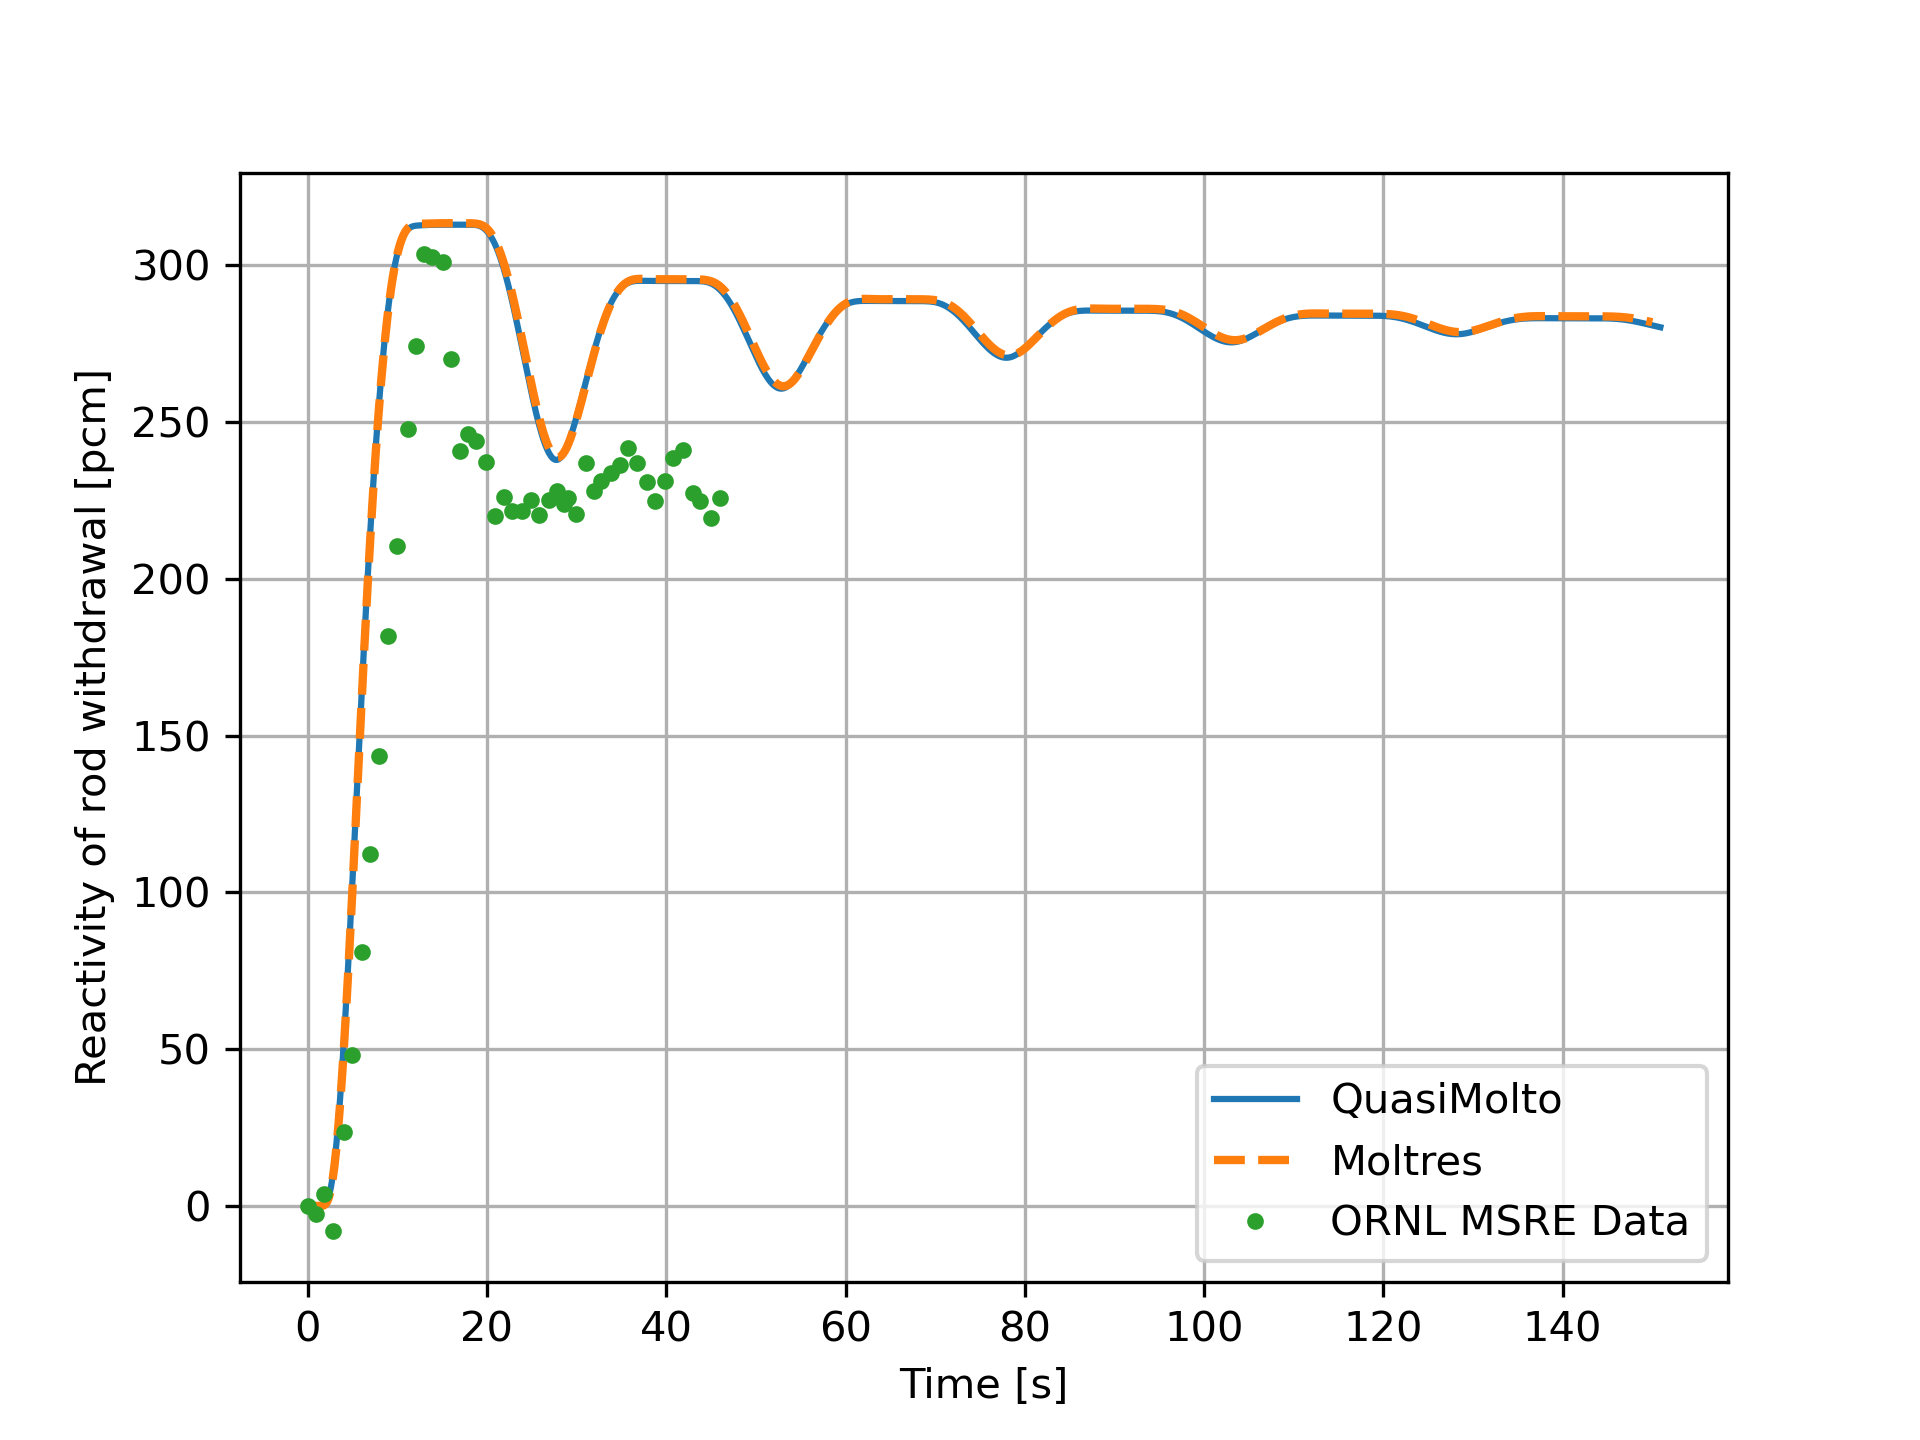
\includegraphics[width=\columnwidth]{start-up-v2-reactivity}
    \caption{Reactivity loss (relative to static no-flow conditions) during the \gls{MSRE} pump
    start-up transient.}
    \label{fig:start-up-reactivity}
  \end{figure}
  \column{5.5cm}
  \textbf{Observations}
  \begin{itemize}
    \item Steep initial reactivity loss due to DNP outflow
    \item Reactivity loss plateaus temporarily before dropping due to DNP reentry
    \item Circulation of the excess DNP cause reactivity oscillations
    \item Oscillations eventually dissipate due to decay of excess DNP
    \item Excellent agreement between Moltres and QuasiMolto
  \end{itemize}
  \end{columns}
\end{frame}

\begin{frame}
  \frametitle{V\&V Study 2: MSRE Pump Start-up \& Coast-Down Transients}
  \textbf{Pump Start-Up Transient Results}
  \begin{columns}
  \column{5.5cm}
  \begin{figure}[t]
    \centering
    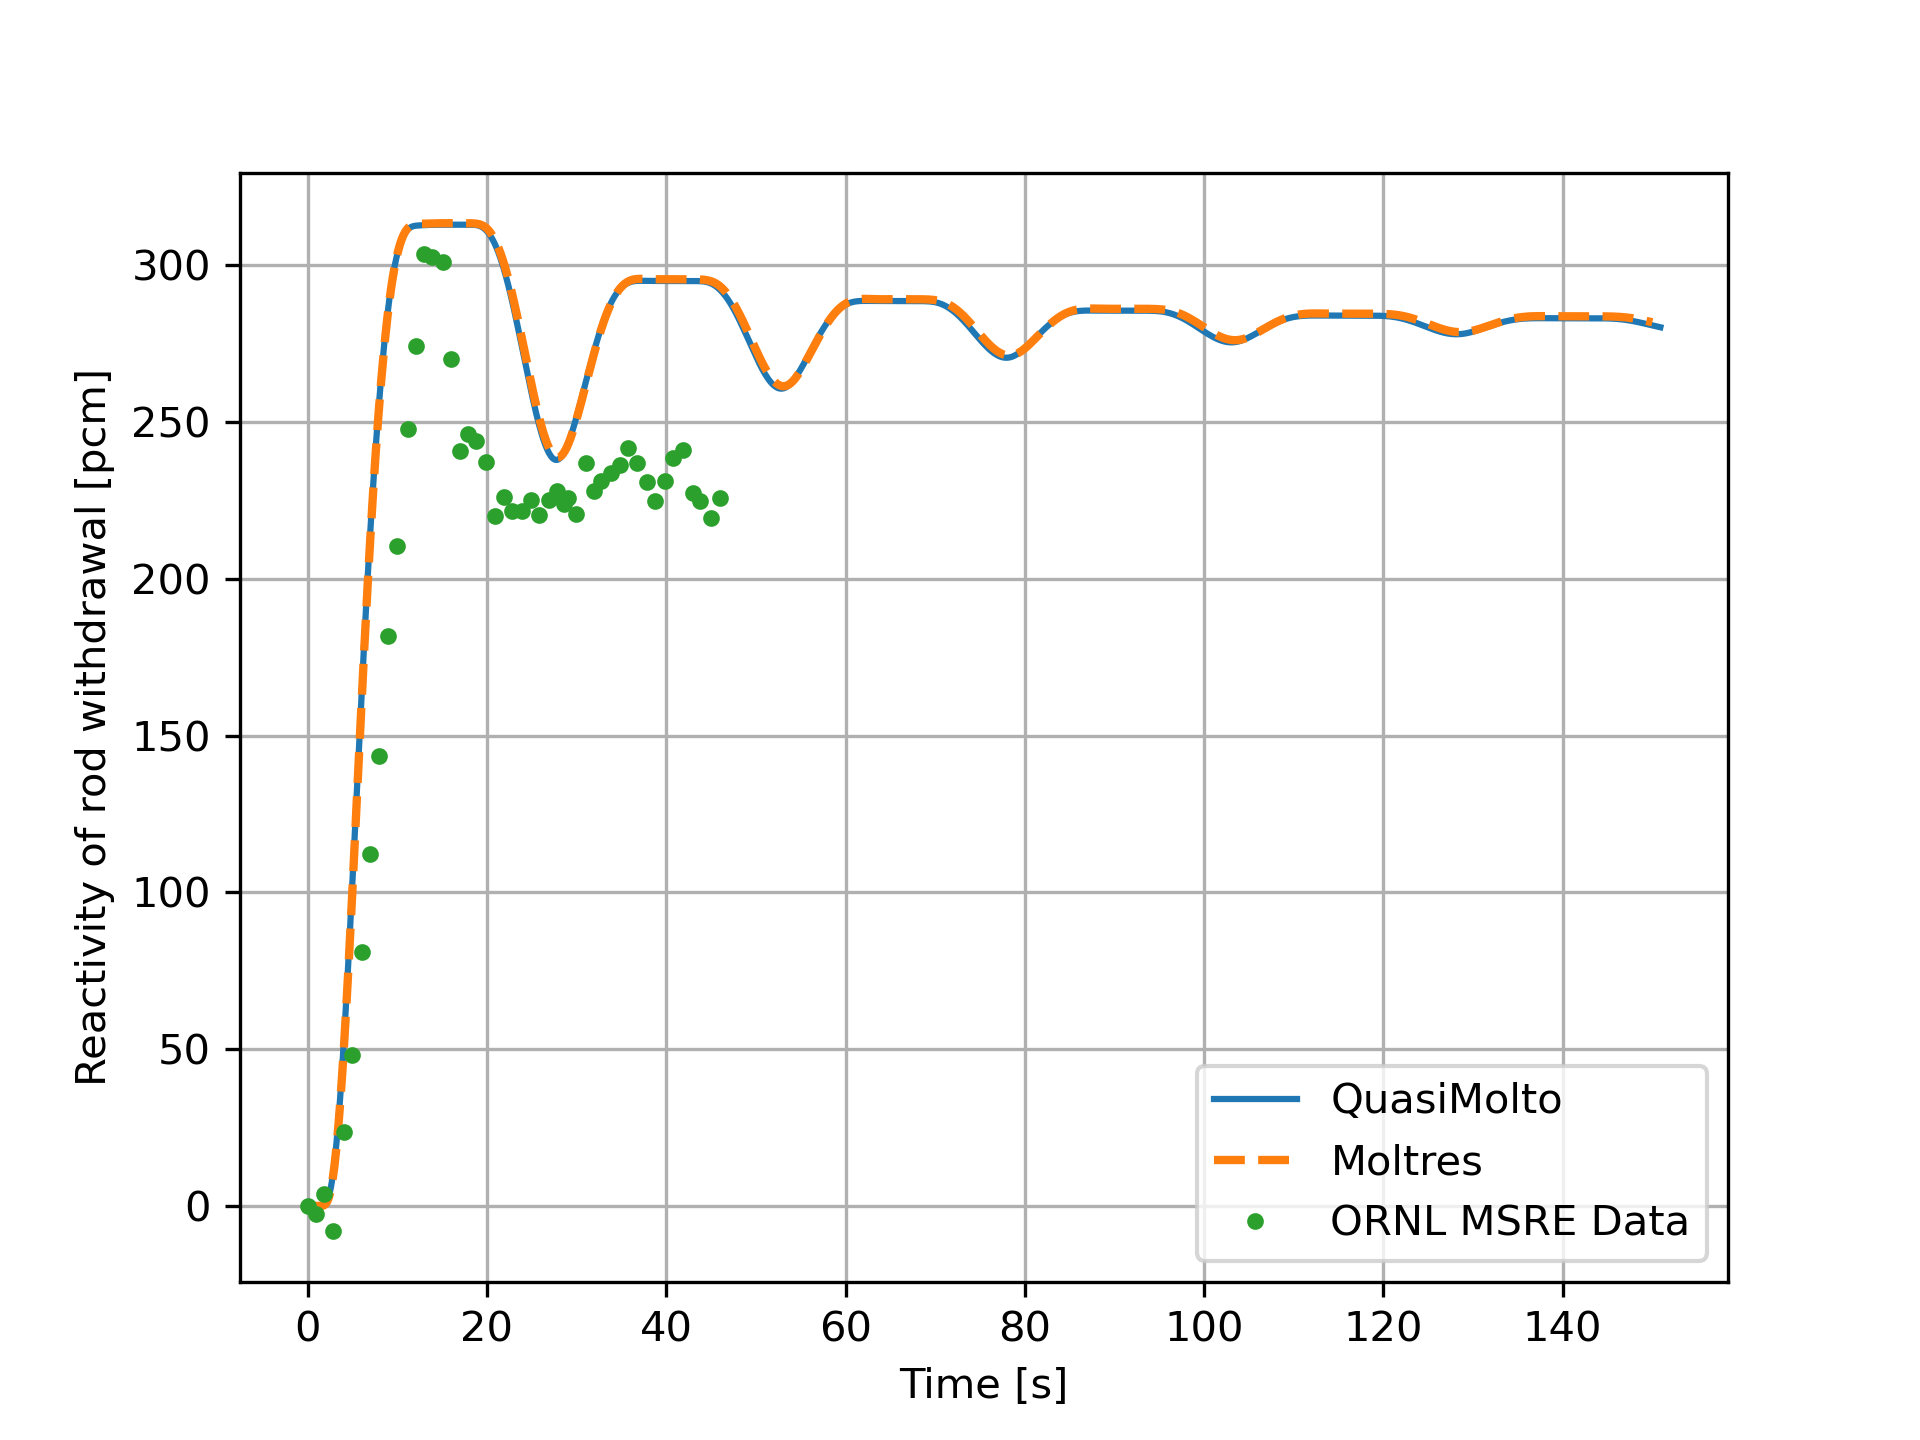
\includegraphics[width=\columnwidth]{start-up-v2-reactivity}
    \caption{Reactivity loss (relative to static no-flow conditions) during the \gls{MSRE} pump
    start-up transient.}
    \label{fig:start-up-reactivity}
  \end{figure}
  \column{5.5cm}
  \textbf{Discrepancies against MSRE Data}
  \begin{itemize}
    \item MSRE reported a smaller final reactivity loss
    \item MSRE did not report a reactivity plateau (due to DNP present in the upper and lower plena)
    \item MSRE did not log significant reactivity oscillations after the first peak
  \end{itemize}
  \end{columns}
\end{frame}

\begin{frame}
  \frametitle{V\&V Study 2: MSRE Pump Start-up \& Coast-Down Transients}
  \textbf{Pump Coast-Down Transient Results}
  \begin{columns}
  \column{5.5cm}
  \begin{figure}[t]
    \centering
    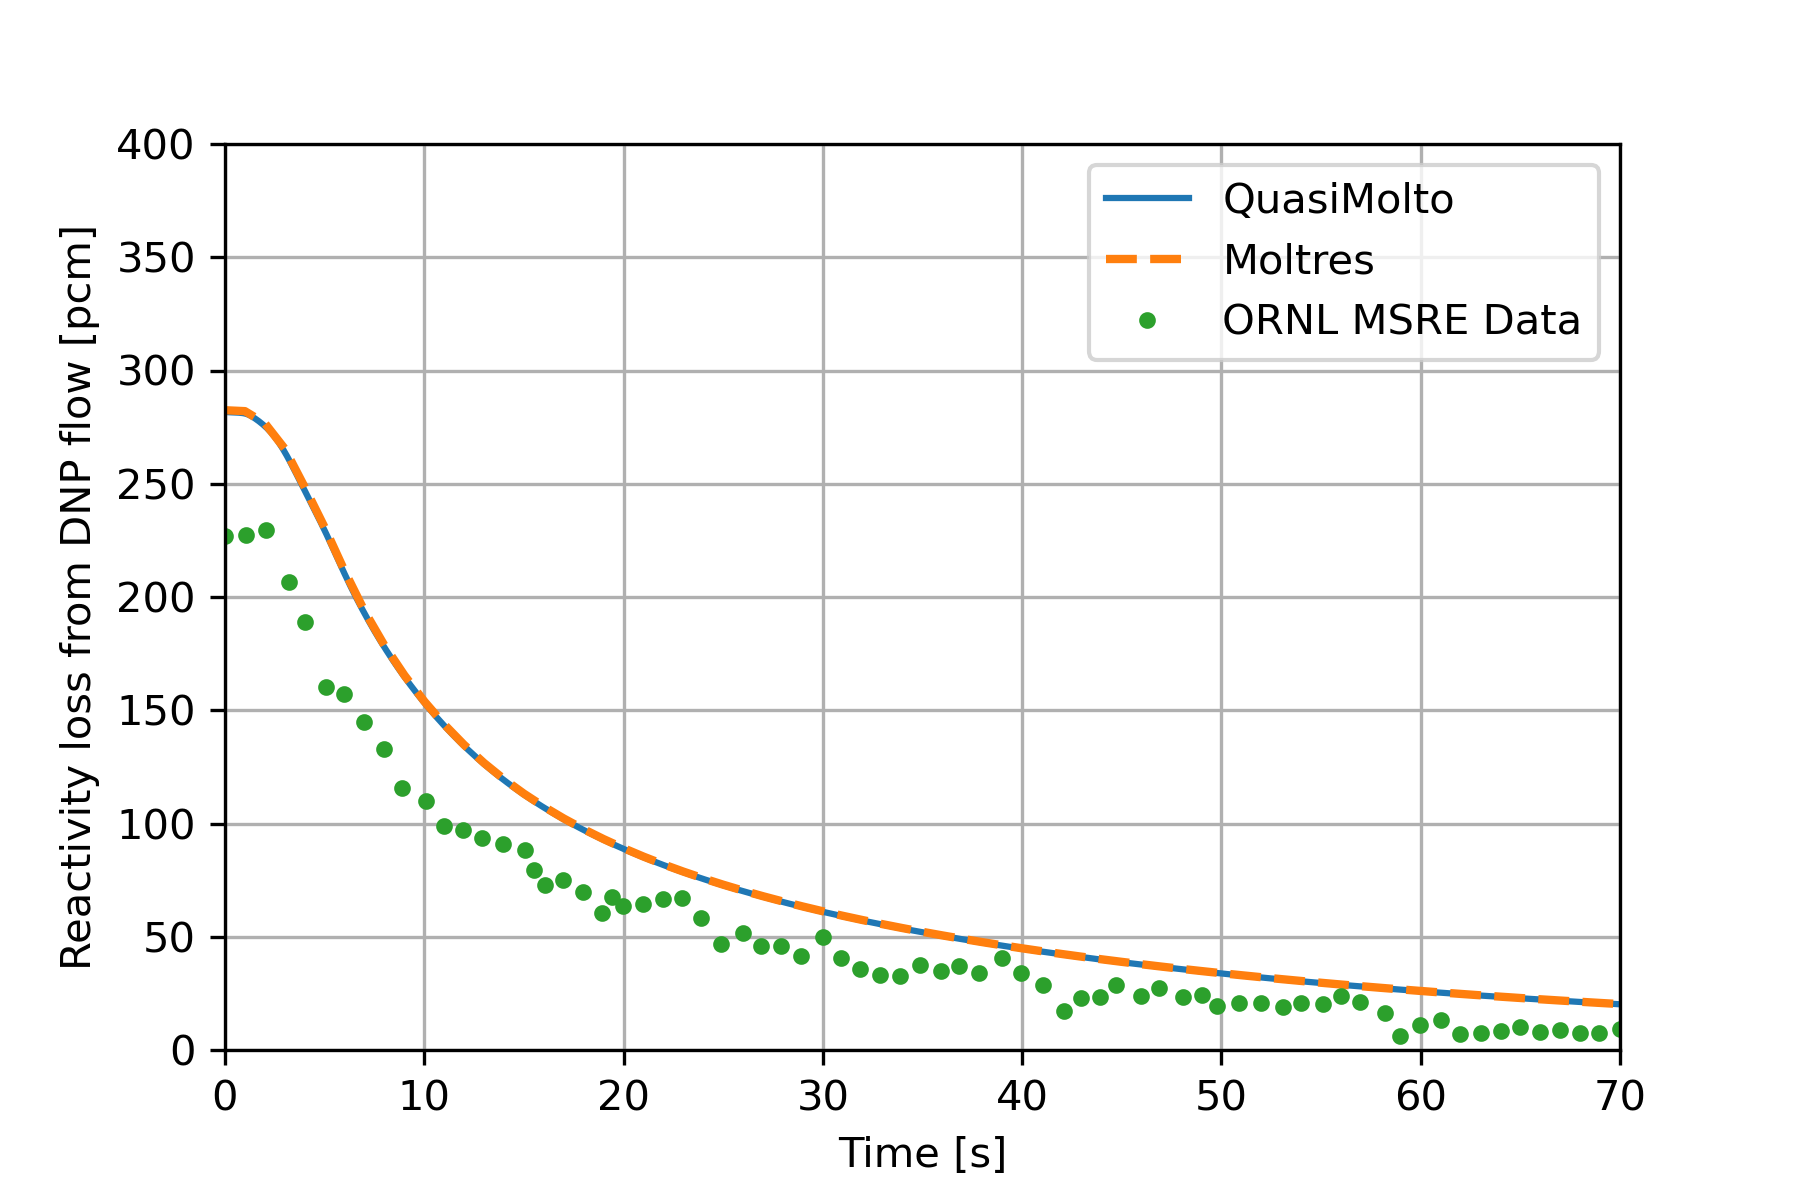
\includegraphics[width=\columnwidth]{coast-down-v2-reactivity}
    \caption{Reactivity loss (relative to static no-flow conditions) during the \gls{MSRE} pump
    coast-down transient.}
    \label{fig:start-up-reactivity}
  \end{figure}
  \column{5.5cm}
  \textbf{Observations}
  \begin{itemize}
    \item Reactivity loss remains briefly stable at the start due to flow inertia
    \item Monotonic decline in reactivity loss over time
  \end{itemize}
  \end{columns}
\end{frame}

\begin{frame}
  \frametitle{V\&V Study 2: MSRE Pump Start-up \& Coast-Down Transients}
  \begin{block}{\textbf{Study Outcome}}
    \begin{itemize}
      \item Moltres and QuasiMolto are highly consistent with each other in their looped DNP flow
        modeling capabilities
      \item Moltres and QuasiMolto reproduced key reactivity behavior in response to varying salt
        flow velocities
      \item Some discrepancies observed between the numerical and experimental results due to the
        omission of upper and lower plena
      \item This study can be used for verifying advection capabilities in other MSR simulation tools
      \item The distinct oscillations serve as valuable reference points to facilitate code-to-code
        comparisons
    \end{itemize}
  \end{block}
\end{frame}

\subsection{Motivation for Turbulence Modeling Implementation}
\begin{frame}
  \frametitle{Motivation for Turbulence Modeling Implementation}
  \textbf{Turbulent Flows in MSRs}
  \begin{itemize}
    \item The Reynolds number of salt flow in MSRs can go up to $10^6$ in the MSFR core
      \cite{fiorina_modelling_2014}.
    \item Turbulent effects expected in MSRs
    \begin{itemize}
      \item Turbulent diffusion of heat and \gls{DNP}
      \item Flow separation and recirculation zones due to abrupt geometry changes
    \end{itemize}
    \item Temperature hotspots may induce thermal stress on structural
      components and temperature-induced reactivity effects.
  \end{itemize}
  \pause
  \begin{block}{\textbf{Area of Improvement for Moltres for MSR Modeling}}
    Moltres does not currently have turbulence modeling capability for simulating
    turbulent flows in MSRs.
  \end{block}
\end{frame}

\subsection{Spalart-Allmaras Turbulence Model in Moltres}
\begin{frame}
  \frametitle{Spalart-Allmaras Turbulence Model in Moltres}
  \begin{block}{\textbf{Why the Spalart-Allmaras Model \cite{spalart_one-equation_1994} for Moltres?}}
    A computationally efficient one-equation model that provides reasonable estimates for wall-bounded
    turbulent flows and is tractable for large problems on small computing clusters.
  \end{block}
  \begin{block}{\textbf{Subobjectives}}
    \textbf{Implementation of a Spalart-Allmaras turbulence model in Moltres}
    \begin{itemize}
      \item Implement a Spalart-Allmaras model in Moltres
      \item Verify and validate the model against reference turbulent flow solutions
    \end{itemize}
  \end{block}
\end{frame}

\begin{frame}
  \frametitle{Spalart-Allmaras Turbulence Model in Moltres}
  \textbf{Spalart-Allmaras Model with Rotation Correction Scheme
  \cite{spalart_one-equation_1994, aupoix_extensions_2003, dacles-mariani_numericalexperimental_1995}}\\
  \\
  Governing equation for the modified dynamic viscosity, $\tilde{\mu}$:
  \begin{multline}
    \rho \frac{\partial\tilde{\mu}}{\partial t} + \rho \mathbf{u}\cdot\nabla\tilde{\mu} = \rho c_{b1}
    \left(1-f_{t2}\right)\tilde{S}\tilde{\mu} + \frac{1}{\sigma}\{\nabla\cdot\left[\left(\mu+
    \tilde{\mu}\right)\nabla\tilde{\mu}\right] + c_{b2}|\nabla\tilde{\mu}|^2\} \\
    - \left(c_{w1}f_w - \frac{c_{b1}}{\kappa^2}f_{t2}\right)\left(\frac{\tilde{\mu}}{d}\right)^2
  \end{multline}
  \begin{align*}
    \shortintertext{where}
      \mu_t &= \tilde{\mu}f_{v1} = \text{turbulent eddy viscosity}, \\
      f_{v1} &= \frac{\chi^3}{\chi^3 + c_{v1}^3}, \\
      \chi &= \frac{\tilde{\mu}}{\mu}.
  \end{align*}
%      \tilde{S} &= \Omega + \frac{\tilde{\nu}}{\kappa^2 d^2} f_{v2}, \\
%      f_{v2} &= 1 - \frac{\chi}{1+\chi f_{v1}}, \\
%      \Omega &= \sqrt{2W_{ij}W_{ij}} = \text{vorticity magnitude}, \\
%      W_{ij} &= \frac{1}{2}\left(\frac{\partial u_i}{\partial x_j} - \frac{\partial u_j}{\partial x_i}
%      \right), \\
%        f_w &= g\left(\frac{1 + c_{w3}^6}{g^6 + c_{w3}^6}\right)^{1/6}, \\
%        g &= r + c_{w2}\left(r^6 - r\right), \\
%        r &= \text{min}\left(\frac{\tilde{\nu}}{\tilde{S}\kappa^2d^2}, 10\right), \\
%        f_{t2} &= c_{t3} \exp{\left(-c_{t4}\chi^2\right)},
%    \end{align*}
%  \shortintertext{and the constants are}
%    \sigma = \frac{2}{3}, \ c_{b1} = 0.1355, \ c_{b2} = 0.622, \ \kappa = 0.41, \
%    c_{w1} = \frac{c_{b1}}{\kappa^2} + \frac{1+c_{b2}}{\sigma}, \nonumber \\
%    c_{w2} = 0.3, \ c_{w3} = 2, \
%    c_{v1} = 7.1, \ c_{t3} = 1.2, \ c_{t4} = 0.5 \ \text{.} \nonumber
\end{frame}

\begin{frame}
  \frametitle{Spalart-Allmaras Turbulence Model in Moltres}
  \begin{block}{\textbf{Model Implementation Details}}
  \begin{itemize}
    \item Built on top of an existing incompressible Navier-Stokes model in MOOSE
    \item Uses Streamline-Upwind/Petrov-Galerkin (SUPG) stabilization scheme for numerical stability
    \item Rotation correction scheme \cite{aupoix_extensions_2003, dacles-mariani_numericalexperimental_1995}
      reduces eddy viscosity in regions of rotational but non-turbulent flow
  \end{itemize}
  \end{block}
  \pause
  \begin{block}{\textbf{Verification \& Validation Tests for the Turbulence Model}}
    \begin{enumerate}
      \item Turbulent Channel Flow Verification Test at Re $\approx 13750$
      \begin{itemize}
        \item Reference results: \gls{DNS} results by Moser et al.\ \cite{moser_direct_1999}
      \end{itemize}
      \item Turbulent Pipe Flow Validation Test at Re $\approx 40000$
      \begin{itemize}
        \item Reference results: Experimental results by Laufer \cite{laufer_structure_1954}
      \end{itemize}
      \item Backward-Facing Step Flow Validation Test
      \begin{itemize}
        \item Reference results: Experimental results by Driver \& Seegmiller \cite{driver_features_1985}
        \& Spalart-Allmaras model results from CFL3D CFD code \cite{krist_cfl3d_1998}
      \end{itemize}
    \end{enumerate}
  \end{block}
\end{frame}

\begin{frame}
  \frametitle{Turbulent Channel Flow Verification Test Results}
  \begin{figure}[htb!]
    \centering
    \begin{subfigure}[b]{0.32\columnwidth}
      \centering
      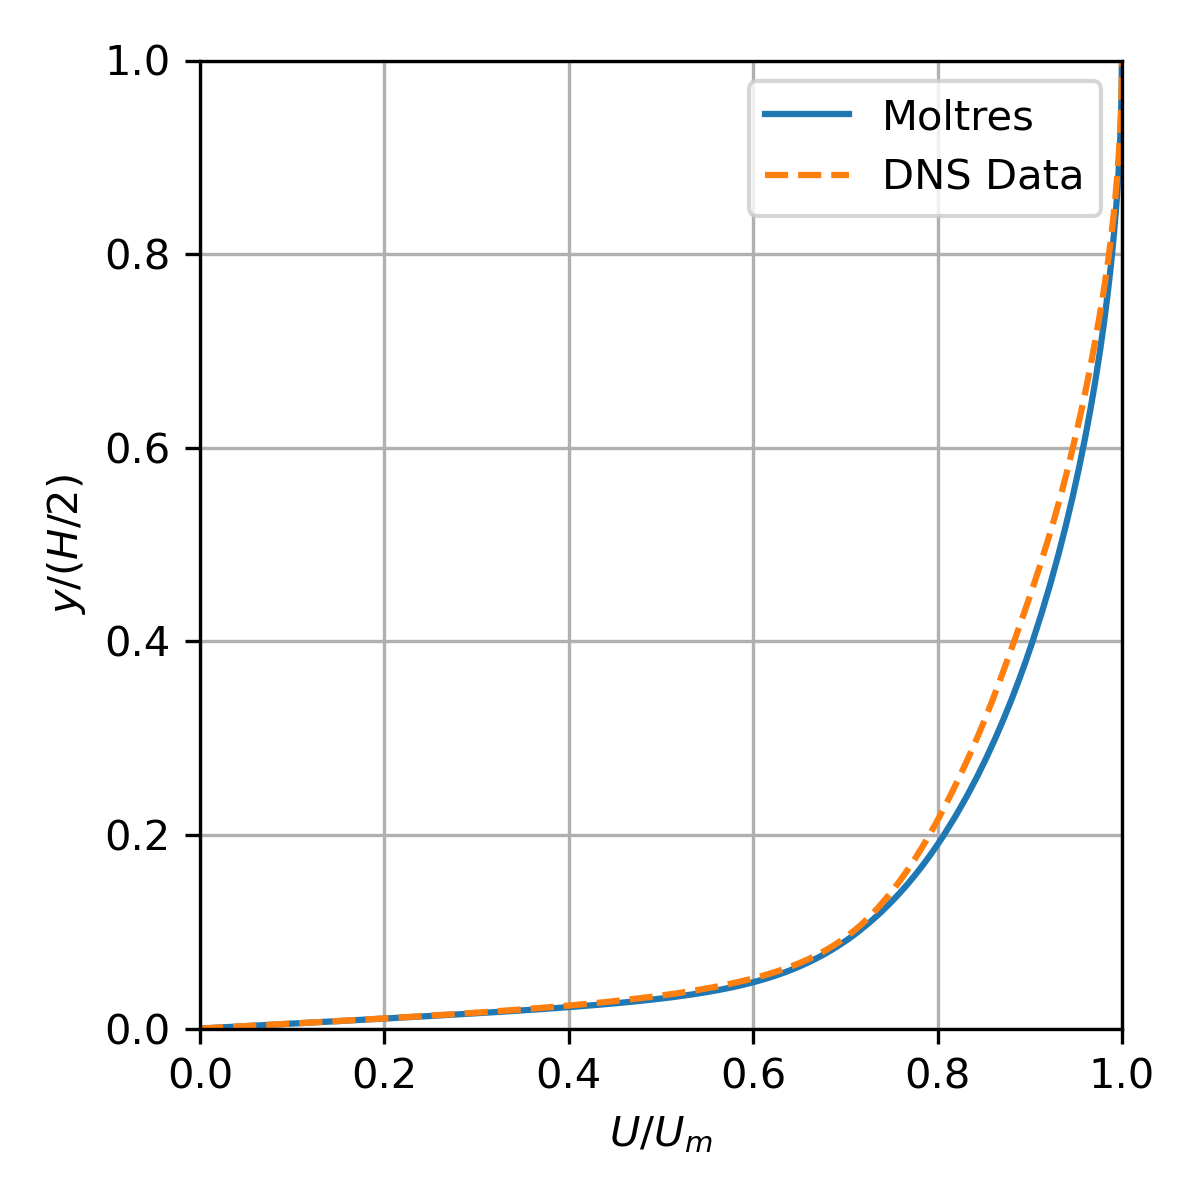
\includegraphics[width=\columnwidth]{channel_vel}
      \caption{Normalized velocity distribution across the channel.}
      \label{fig:channel-vel}
    \end{subfigure}
    \hfill
    \begin{subfigure}[b]{0.32\columnwidth}
      \centering
      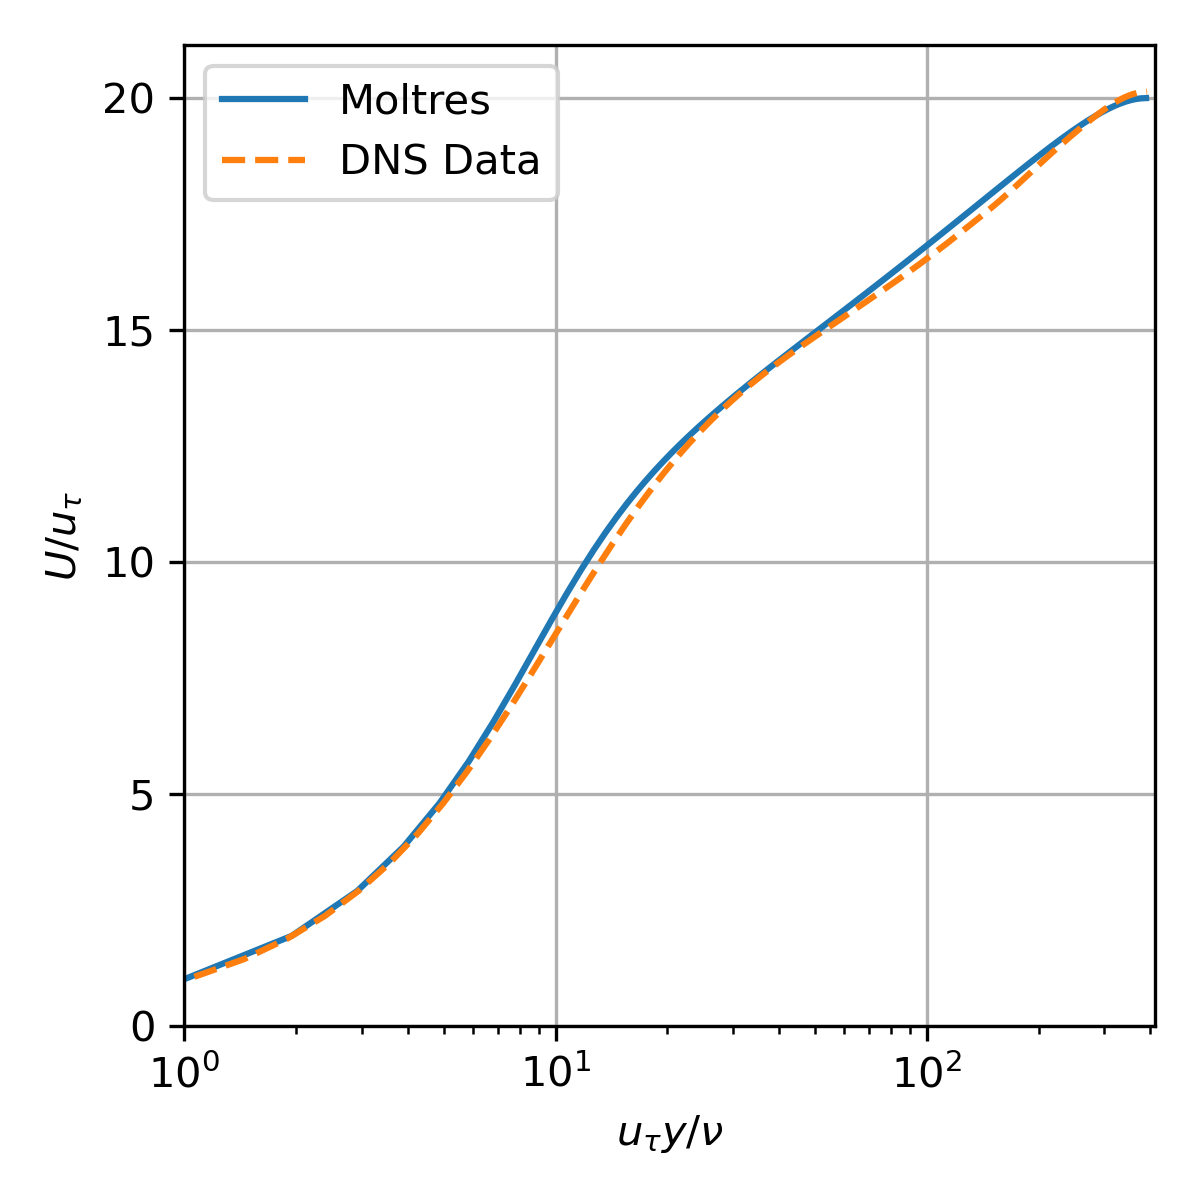
\includegraphics[width=\columnwidth]{channel_nondim}
      \caption{Dimensionless velocity vs.\ dimensionless wall distance.}
      \label{fig:channel-nondim}
    \end{subfigure}
    \begin{subfigure}[b]{0.32\columnwidth}
      \centering
      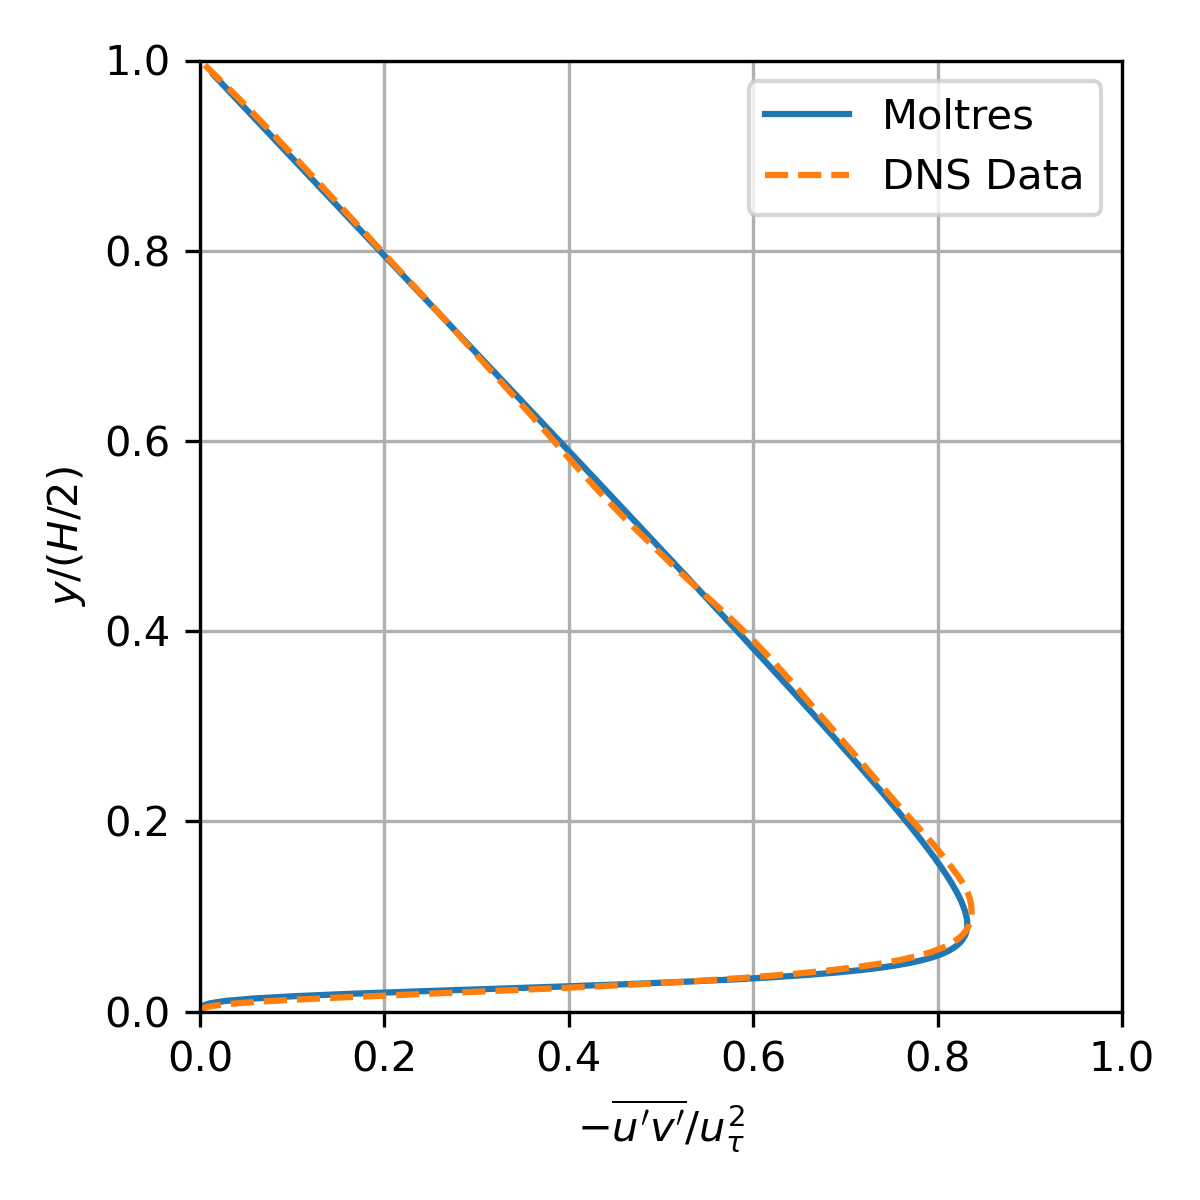
\includegraphics[width=\columnwidth]{channel_stress}
      \caption{Normalized stress distribution across the channel.}
      \label{fig:channel-stress}
    \end{subfigure}
    \caption{Comparison of turbulent channel flow results at Re$_\tau\approx395$ against reference
    \gls{DNS} results \cite{moser_direct_1999}.}
    \label{fig:channel-verification}
  \end{figure}
  \vspace{.1cm}

  $\Rightarrow$ The Moltres Spalart-Allmaras model results are consistent with reference DNS channel flow data.
\end{frame}

\begin{frame}
  \frametitle{Turbulent Pipe Flow Validation Test Results}
  \begin{figure}[htb]
    \centering
    \begin{subfigure}[b]{0.32\columnwidth}
      \centering
      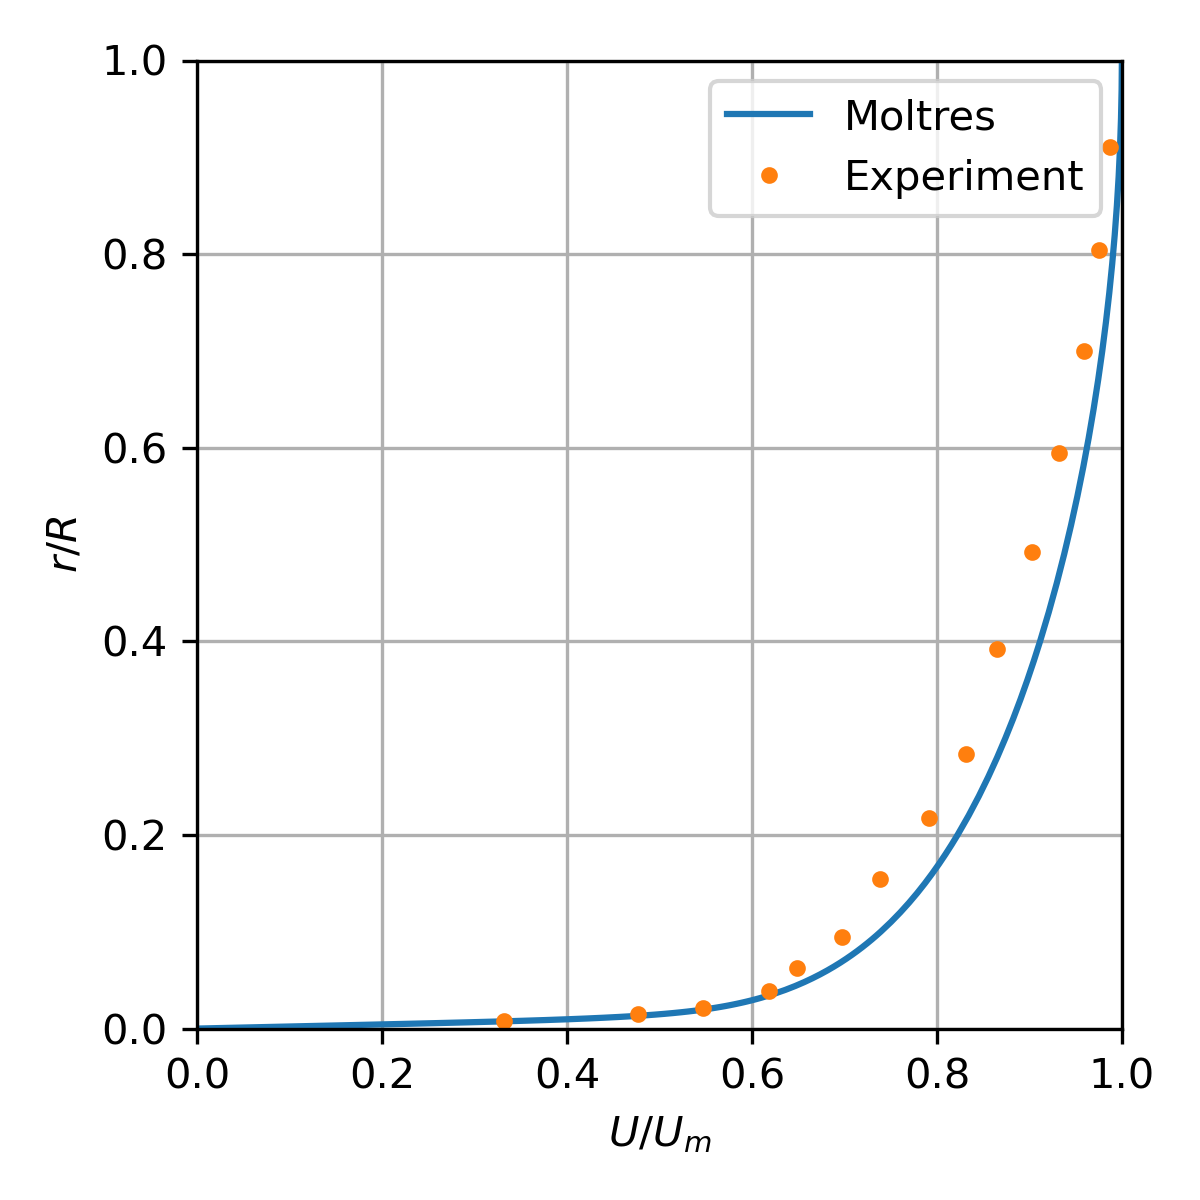
\includegraphics[width=\columnwidth]{pipe_vel}
      \caption{Normalized velocity distribution across the pipe.}
      \label{fig:pipe-vel}
    \end{subfigure}
    \hfill
    \begin{subfigure}[b]{0.32\columnwidth}
      \centering
      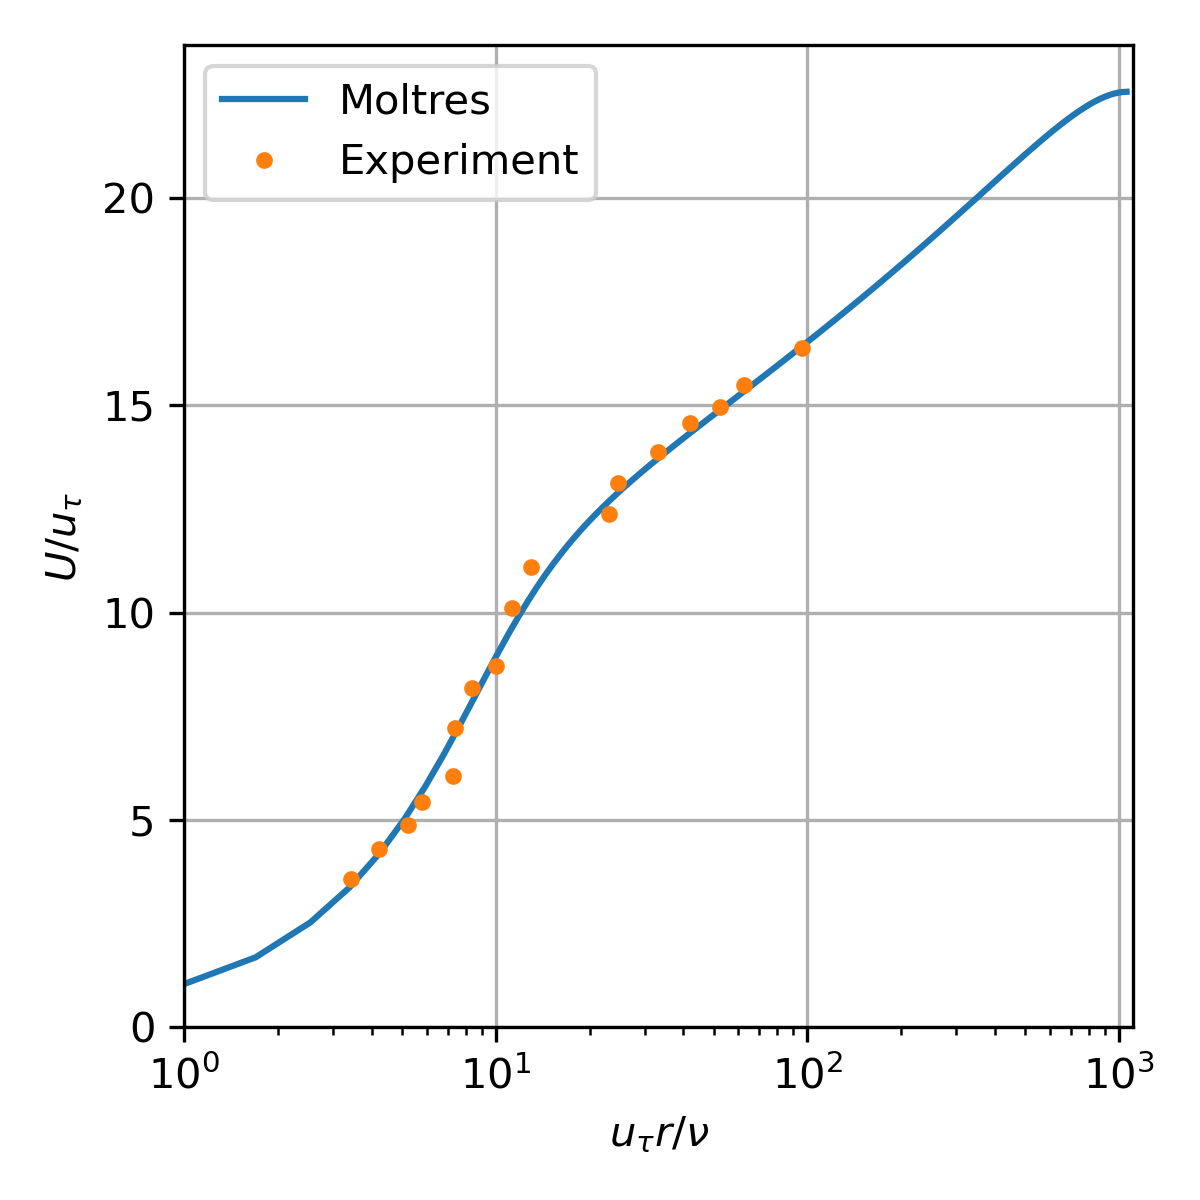
\includegraphics[width=\columnwidth]{pipe_nondim}
      \caption{Dimensionless velocity vs.\ dimensionless wall distance}
      \label{fig:pipe-nondim}
    \end{subfigure}
    \begin{subfigure}[b]{0.32\columnwidth}
      \centering
      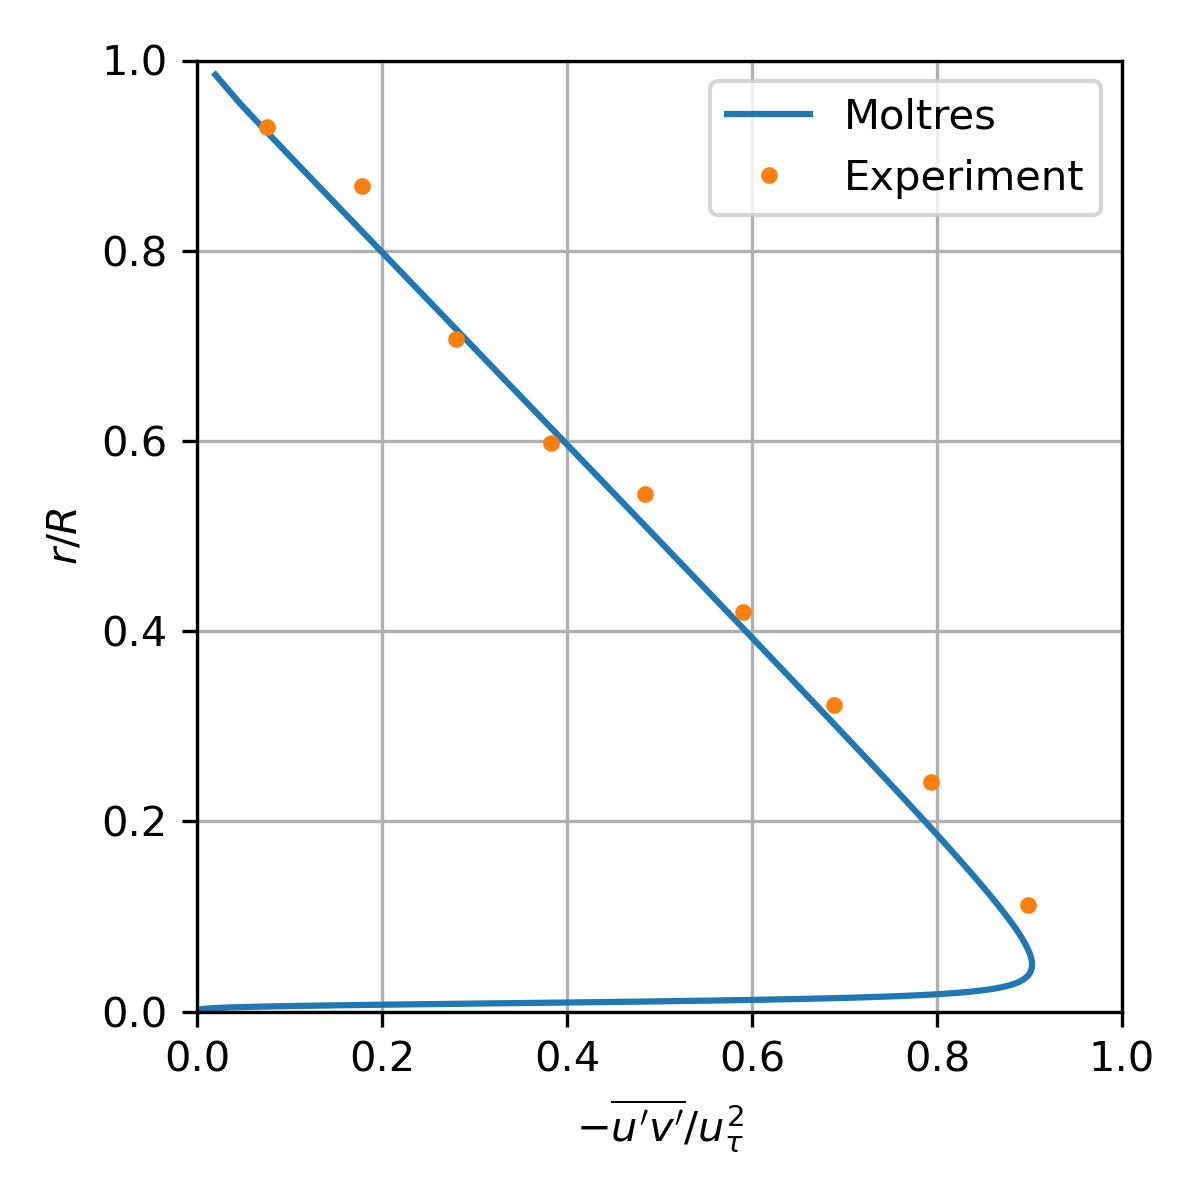
\includegraphics[width=\columnwidth]{pipe_stress}
      \caption{Normalized turbulent shear stress across the pipe.}
      \label{fig:pipe-stress}
    \end{subfigure}
    \caption{Comparison of turbulent pipe flow results at Re $\approx 40000$ against reference
    experimental data \cite{laufer_structure_1954}.}
    \label{fig:pipe-verification}
  \end{figure}
  \vspace{.1cm}

  $\Rightarrow$ The Moltres Spalart-Allmaras model results are consistent with reference experimental pipe flow data.
\end{frame}

\begin{frame}
  \frametitle{Backward-Facing Step Flow Validation Test Setup}
  \begin{columns}
    \column{5.5cm}
    \begin{figure}[h]
      \centering
      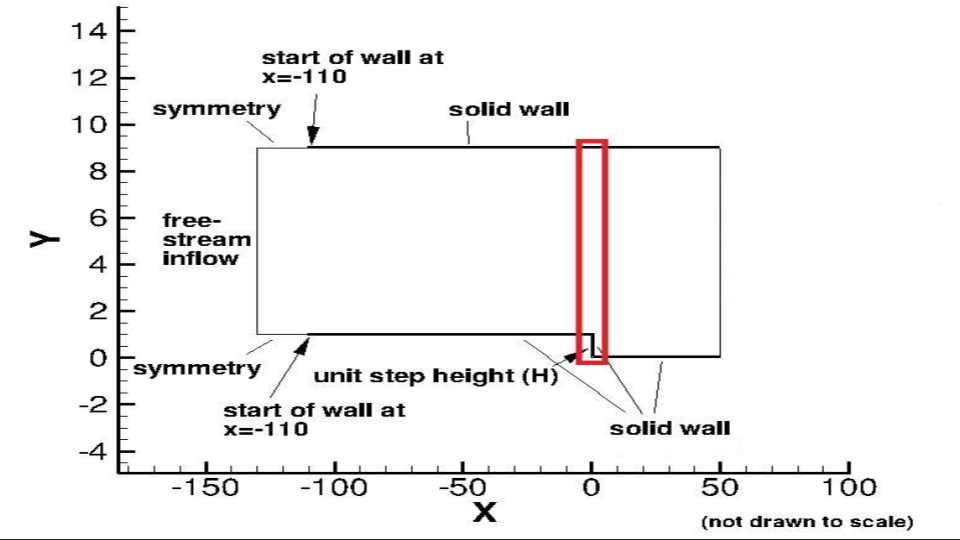
\includegraphics[width=\columnwidth]{backstep-geom-pres}
      \caption{Backward step geometry for the turbulent BFS flow verification test. The red box indicates
      the region shown by the close-up view in Figure \ref{fig:bfs-mesh}.}
      \label{fig:backstep-geom}
    \end{figure}
    \column{5.5cm}
    \begin{figure}[h]
      \centering
      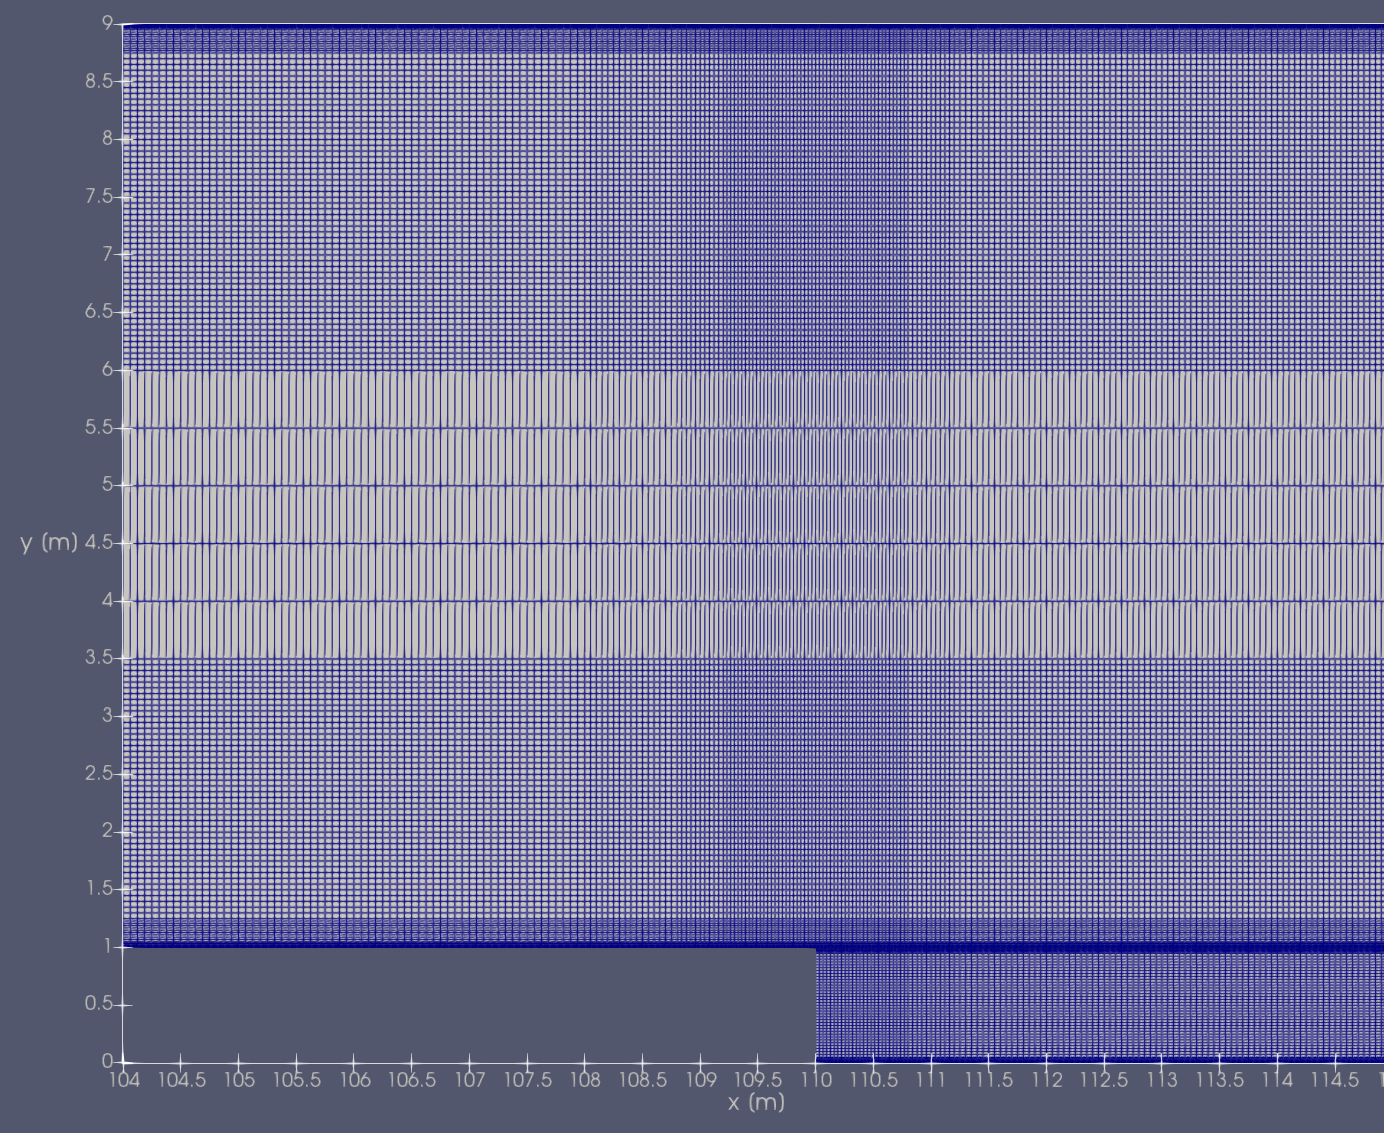
\includegraphics[width=\columnwidth]{bfs_mesh}
      \caption{Close-up view of the mesh for the BFS flow test. The step is situated at $x=110$ m
      with a height of $H=1$ m.}
      \label{fig:bfs-mesh}
    \end{figure}
  \end{columns}
\end{frame}

\begin{frame}
  \frametitle{Backward-Facing Step Flow Validation Test Results}
  \begin{columns}
    \column{5.5cm}
    \begin{figure}[htb!]
      \centering
      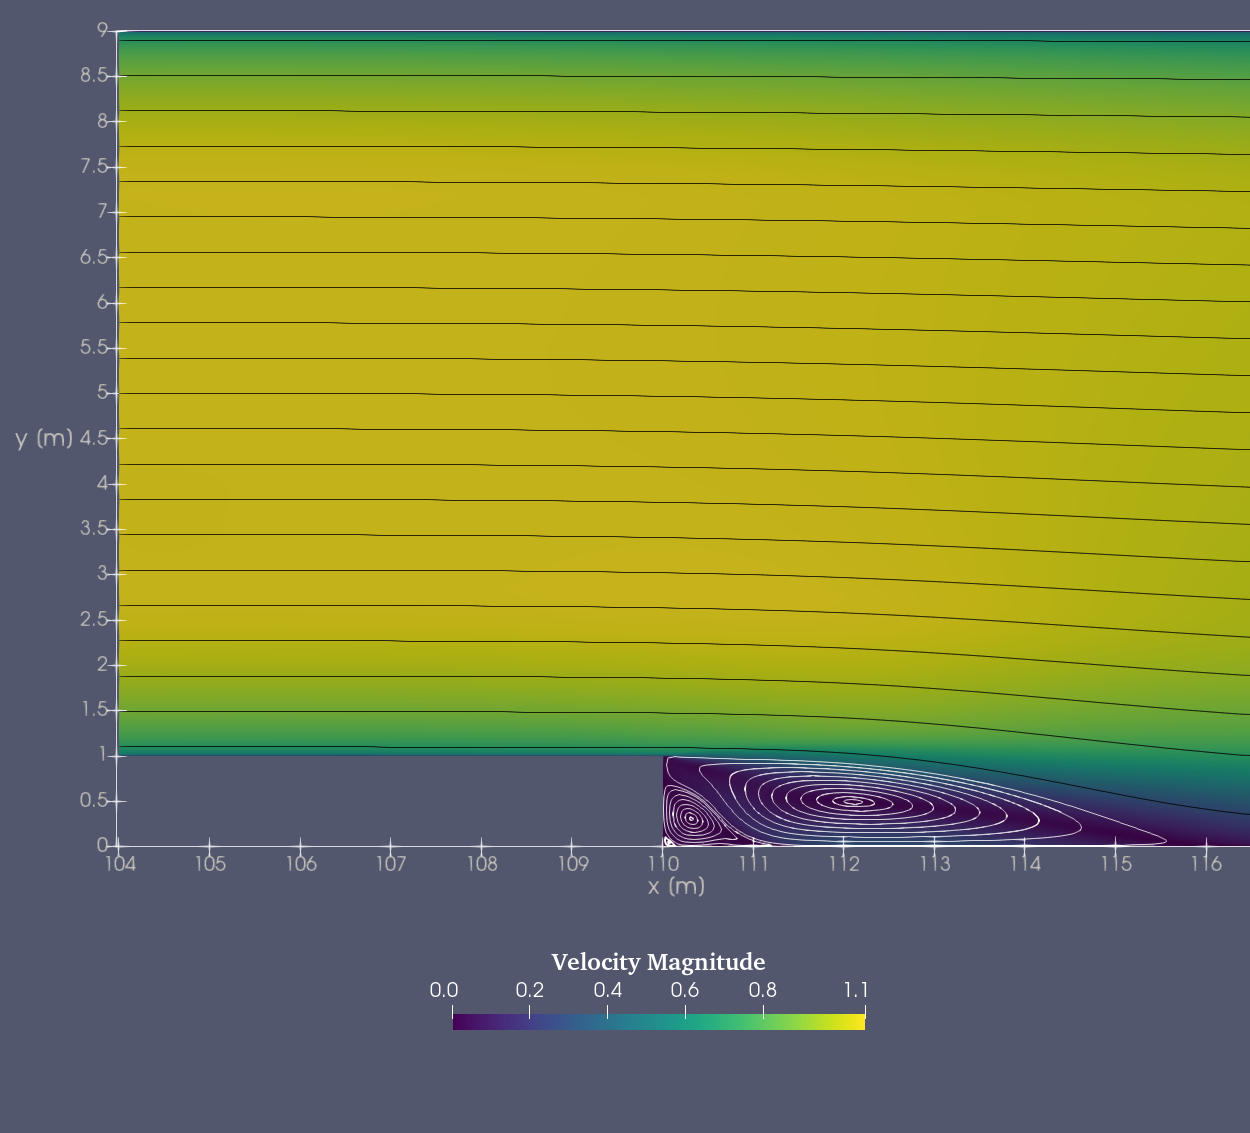
\includegraphics[width=\columnwidth]{bfs}
      \caption{Velocity magnitude distribution and streamlines around the backward-facing step. The
      streamlines illustrate the primary and secondary recirculation zones.}
      \label{fig:bfs}
    \end{figure}
    \column{5.5cm}
    \begin{table}[htb]
      \centering
      \scriptsize
      \caption{BFS flow reattachment length estimates normalized by step height $H$.}
      \begin{tabular}{l S[table-format=1.2(2)]}
        \toprule
        Source & {Reattachment length [-]} \\
        \midrule
        Experimental data & 6.26(10) \\
        CFL3D & 6.1 \\
        Moltres & 6.36 \\
        \bottomrule
      \end{tabular}
      \label{table:bfs-reattach}
    \end{table}
    \vspace{.1cm}

    $\Rightarrow$ Moltres is consistent with experimental data (within uncertainty range) while CFL3D
    falls outside the uncertainty range.
  \end{columns}
\end{frame}

\begin{frame}
  \frametitle{Backward-Facing Step Flow Validation Test Results}
  \begin{columns}
    \column{11.5cm}
    \begin{figure}[htb]
      \centering
      \begin{subfigure}[t]{0.32\columnwidth}
        \centering
        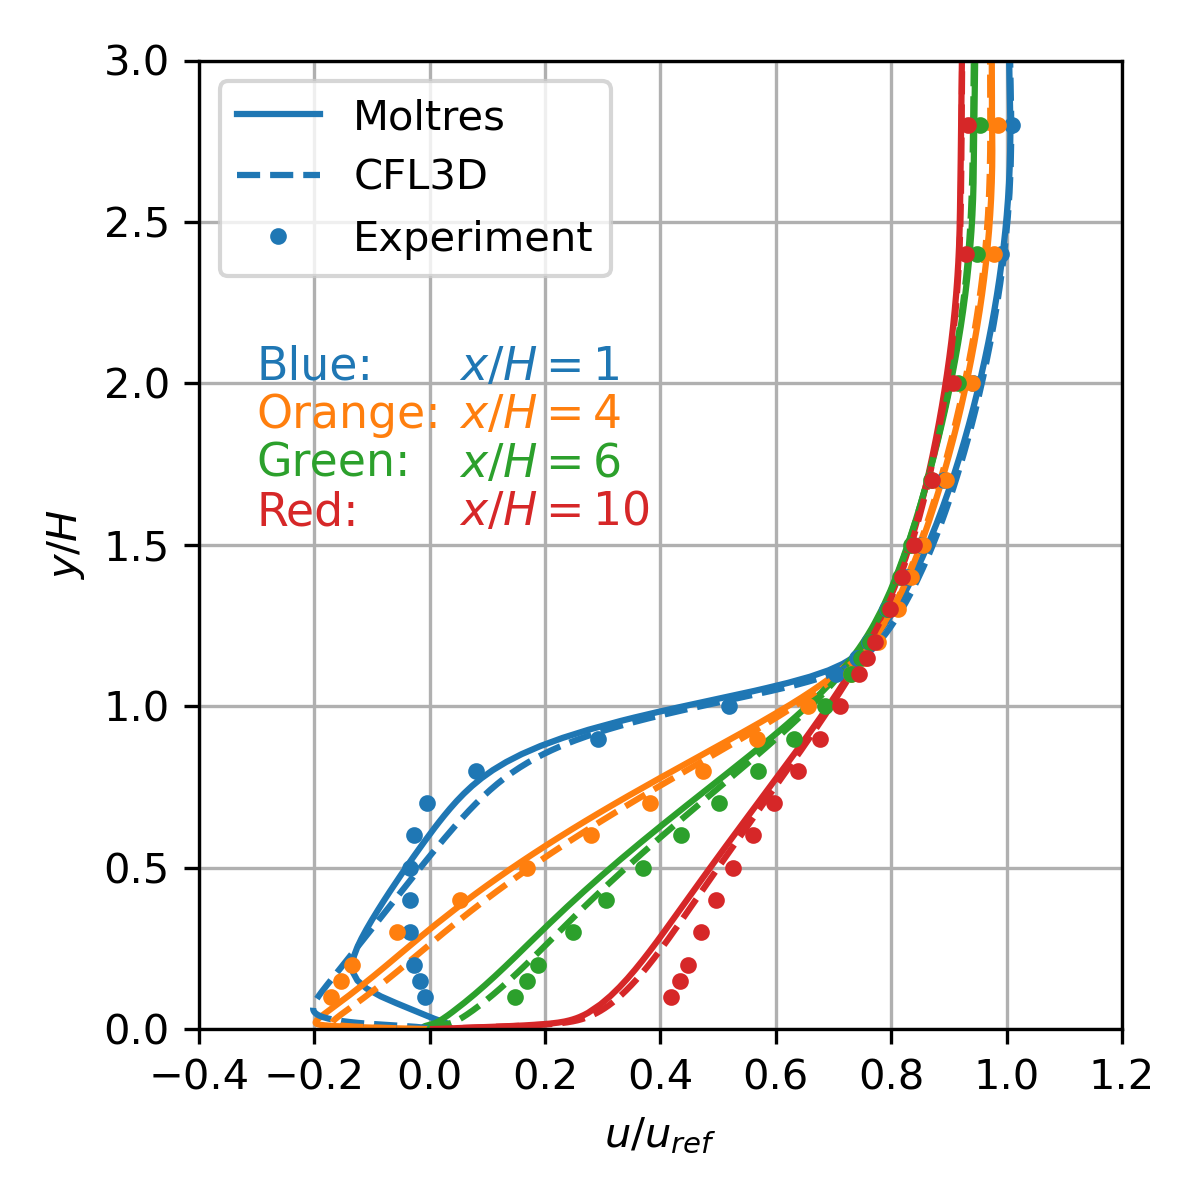
\includegraphics[width=\columnwidth]{bfs_downstream_vel}
        \caption{Normalized velocity distributions downstream of step.}
        \label{fig:bfs-downstream}
      \end{subfigure} %\hfill \\
      \begin{subfigure}[t]{0.32\columnwidth}
        \centering
        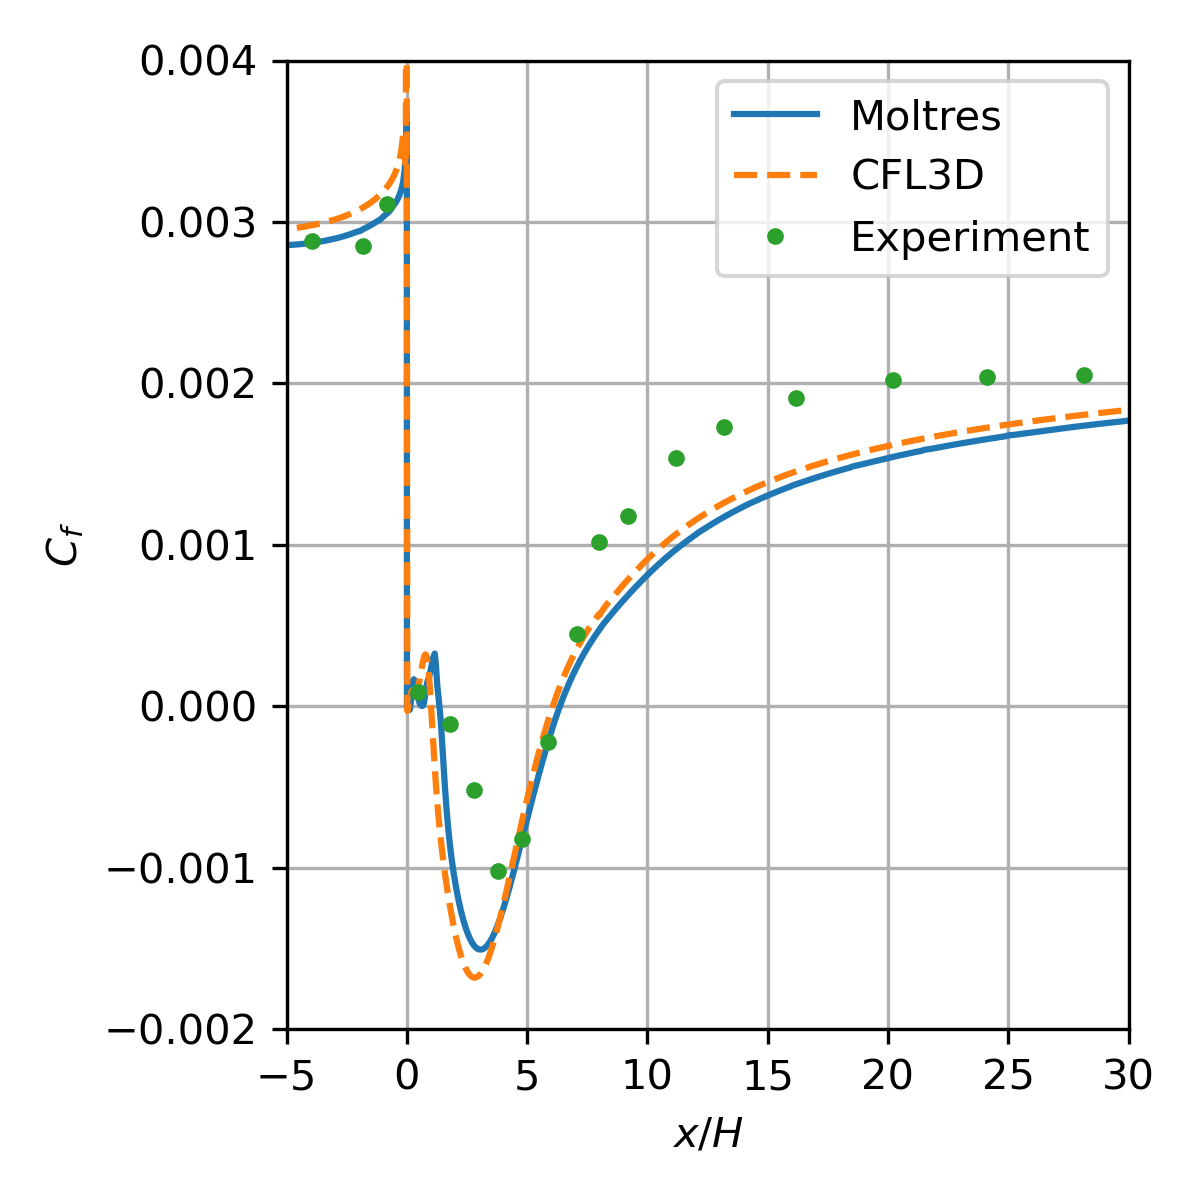
\includegraphics[width=\columnwidth]{bfs_cf}
        \caption{Skin friction coefficient along the bottom wall.}
        \label{fig:bfs-cf}
      \end{subfigure}
      \begin{subfigure}[t]{0.32\columnwidth}
        \centering
        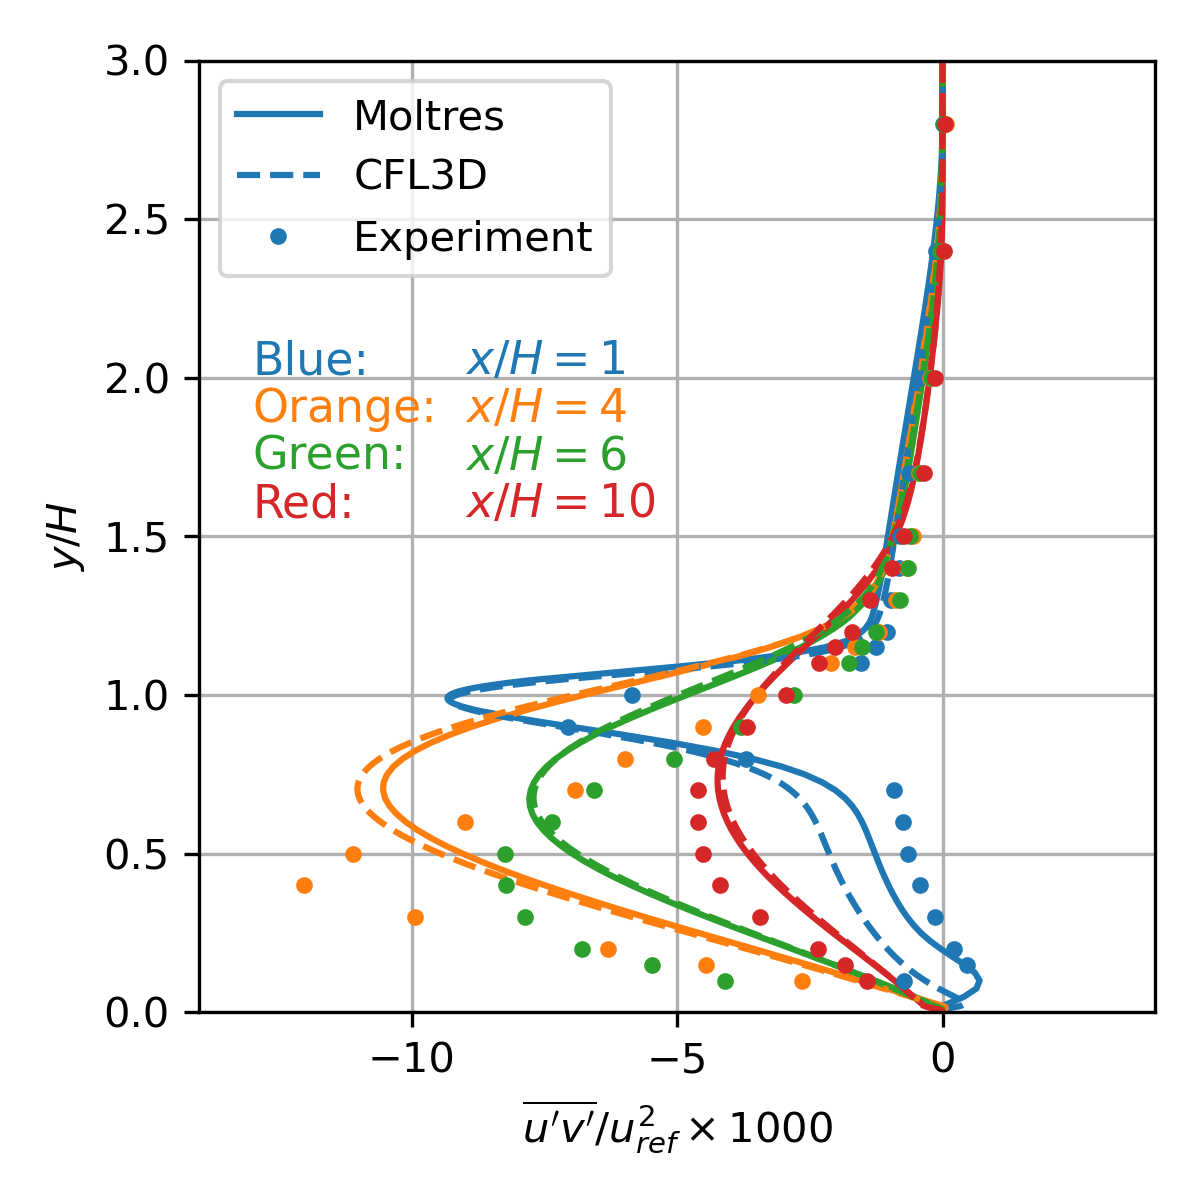
\includegraphics[width=\columnwidth]{bfs_stress}
        \caption{Normalized turbulent shear stress downstream
        of step.}
        \label{fig:bfs-stress}
      \end{subfigure}
      \caption{Comparison of backward facing step flow results against reference
      experimental data and computational data from CFL3D. $x/H$ values are normalized horizontal
      distances relative to the step.}
      \label{fig:bfs-plots}
    \end{figure}
  \end{columns}
  \begin{itemize}
    \item Minor discrepancies between numerical and experimental data typical of RANS-based turbulence models.
    \item Moltres provides more accurate measurements along $x/H=1$ than CFL3D.
  \end{itemize}
\end{frame}

\begin{frame}
  \frametitle{Spalart-Allmaras Turbulence Model in Moltres}
  \begin{block}{\textbf{Spalart-Allmaras Model V\&V Test Summary}}
    \begin{itemize}
      \item Good agreement between Moltres and reference solutions in the turbulent channel and pipe
        flow tests.
      \item Good agreement between Moltres and CFL3D in the backward-facing step flow test.
      \item Some discrepancy between Moltres and experimental data in the backward-facing step flow
        test, but Moltres performed better than CFL3D at predicting flow reattachment length and
        velocity/stress distributions along $x/H=1$.
    \end{itemize}
  \end{block}
\end{frame}


\section{Objective 2: Hybrid $S_N$-Diffusion Method}
\subsection{Motivation}
\begin{frame}
  \frametitle{Control Rods in MSRs}
  \begin{columns}
    \hfill
    \column[t]{5cm}
    \vspace{.2cm}
    \begin{figure}
      \centering
      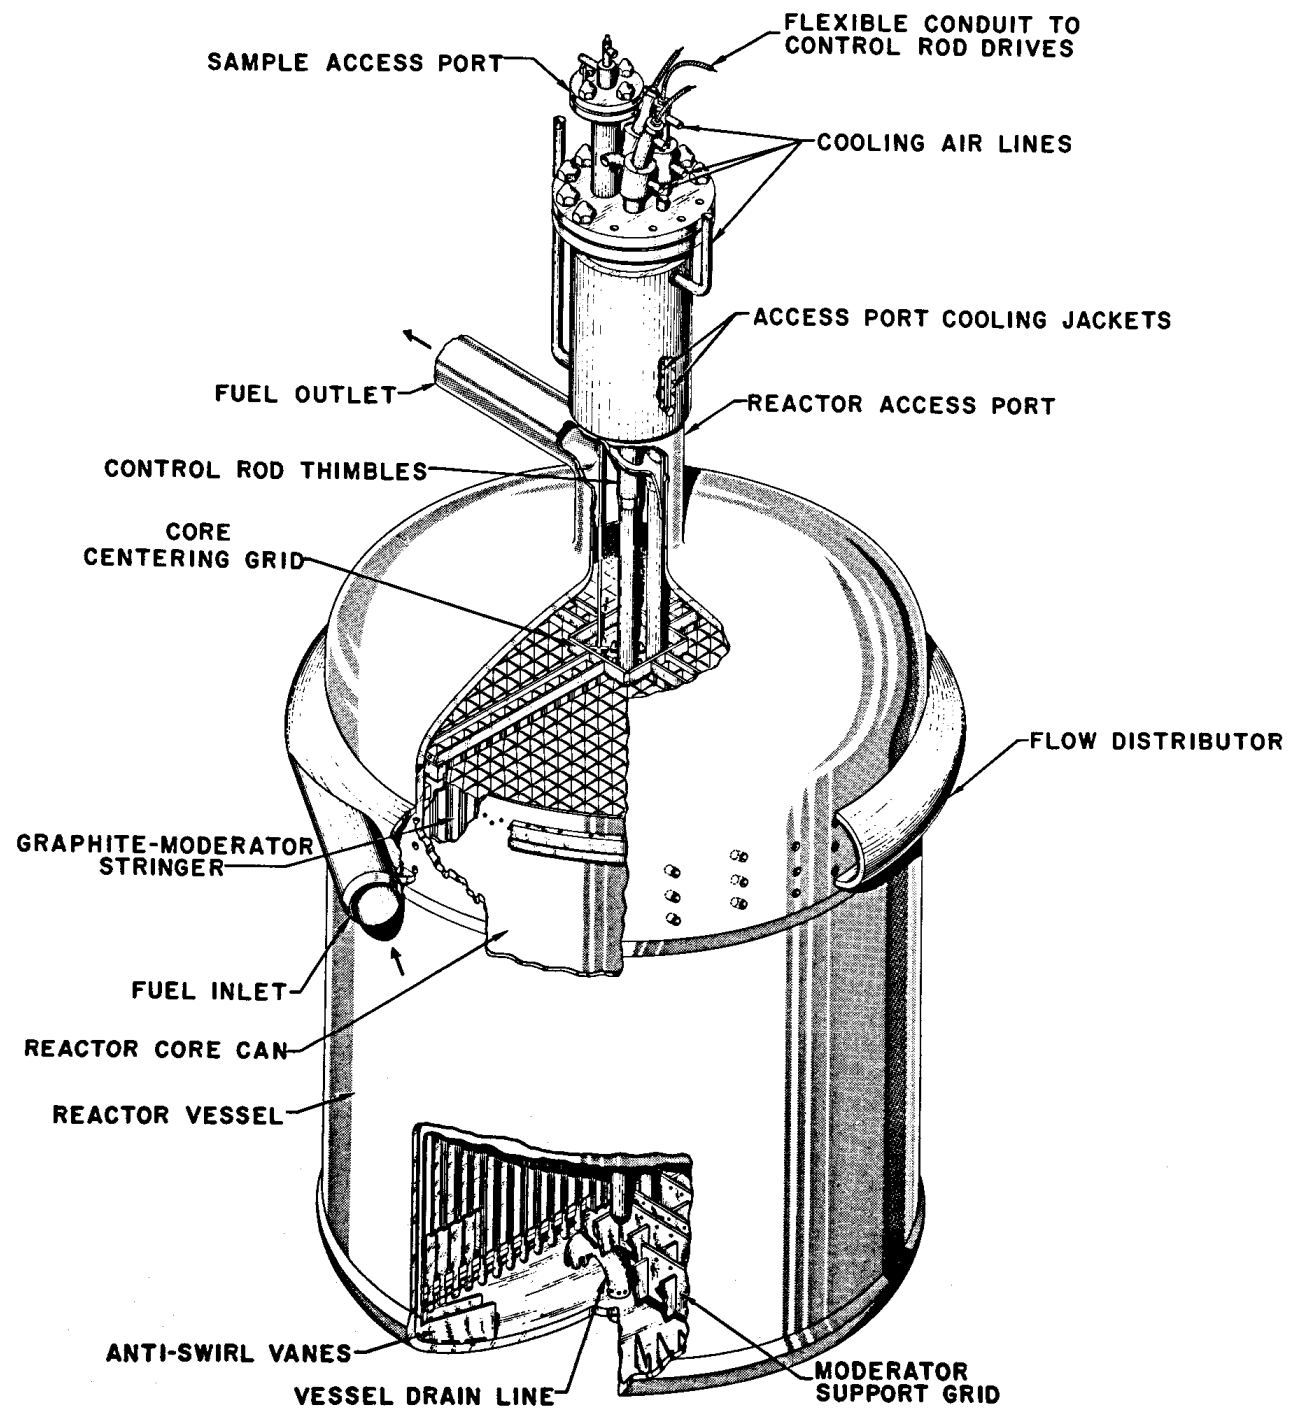
\includegraphics[width=\columnwidth]{images/msre-cutout}
      \caption{\footnotesize MSRE reactor vessel \cite{robertson_msre_1965}}
    \end{figure}
    \hfill
    \column[t]{6cm}
    \begin{figure}
      \centering
      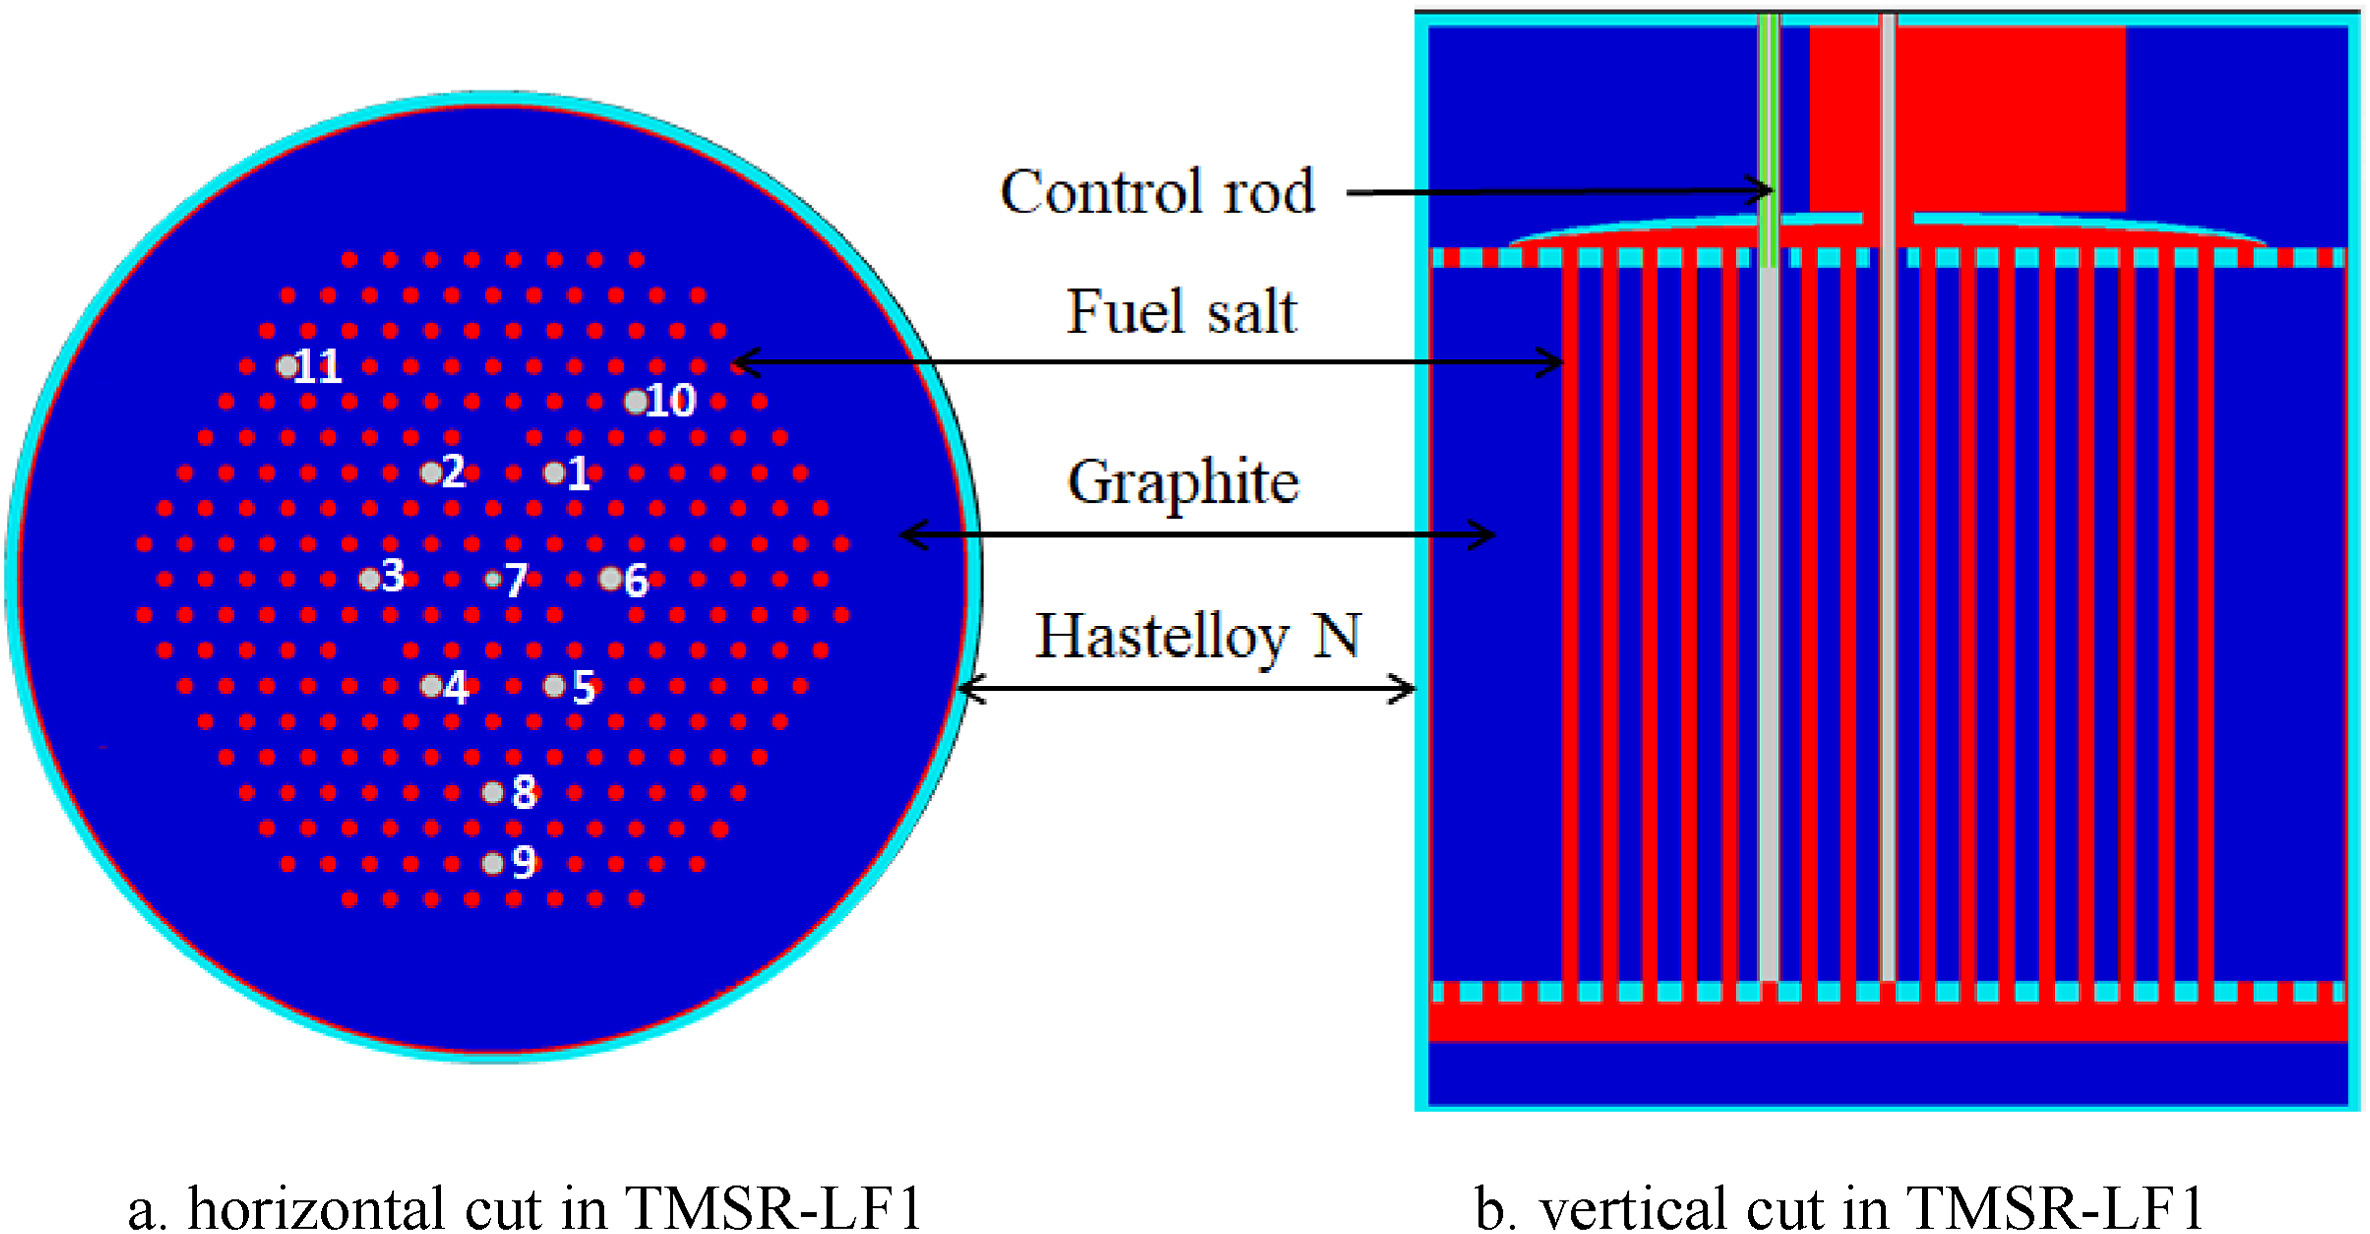
\includegraphics[width=.8\columnwidth]{images/tmsr}
      \caption{\footnotesize Cross-sectional views of the TMSR-LF1
      \cite{liu_sensitivityuncertainty_2020}}
    \end{figure}
    \begin{figure}
      \centering
      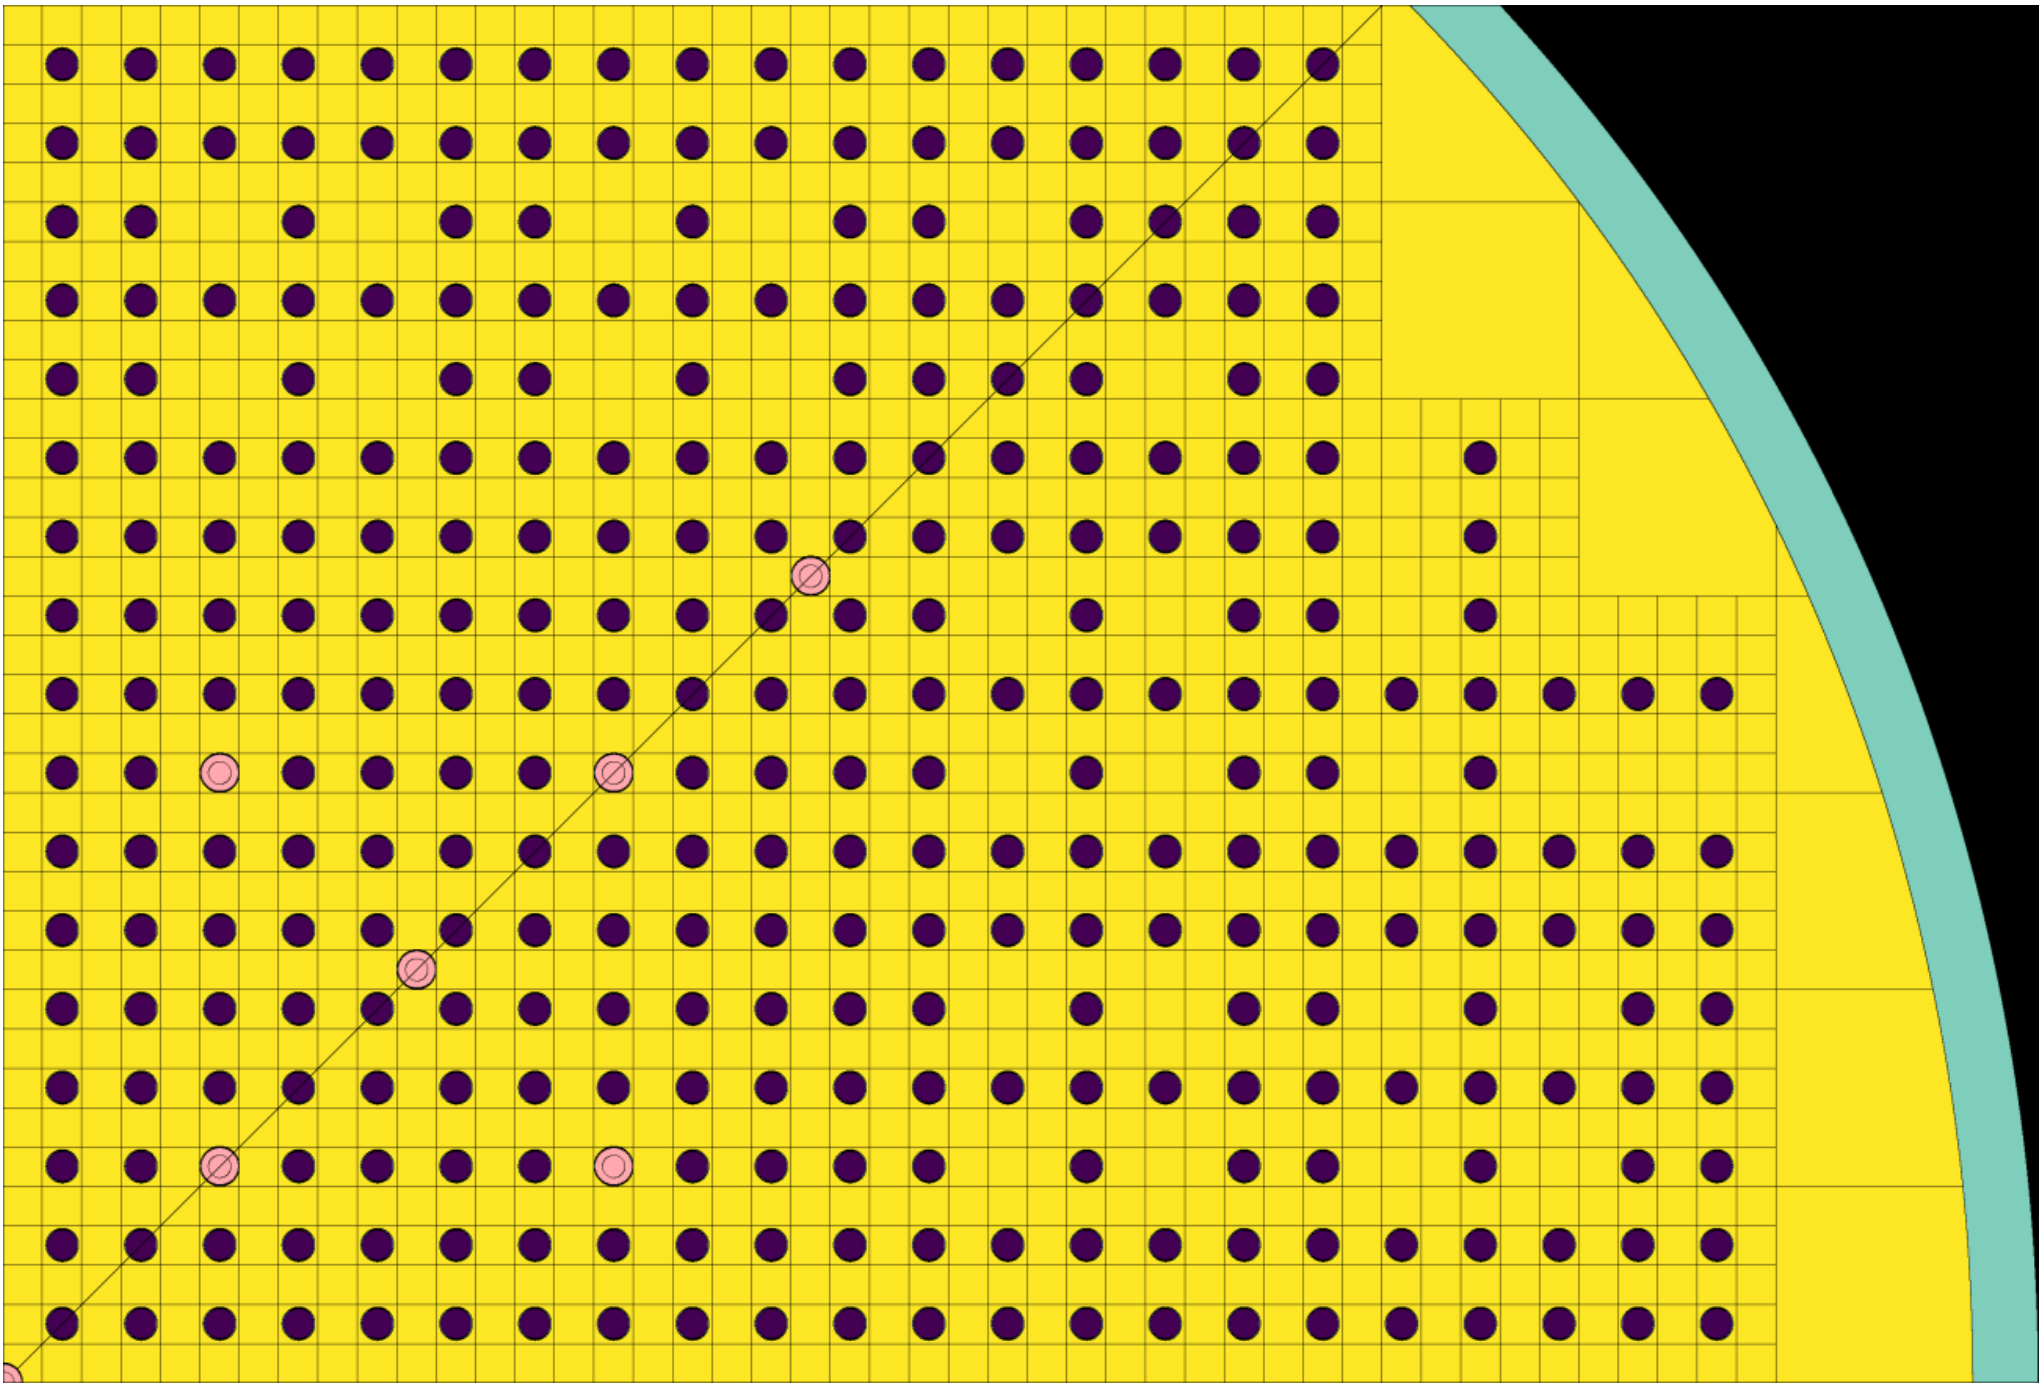
\includegraphics[width=.5\columnwidth]{images/tap-msr-rods}
      \caption{\footnotesize Cross-sectional view of the TAP MSR \cite{lee_neutronics_2020}}
    \end{figure}
    \hfill
  \end{columns}
\end{frame}

\begin{frame}
  \frametitle{Control Rods in MSRs}
  \textbf{Control rods provide a means of controlling the fission rate in nuclear reactors.} 
  \begin{itemize}
    \item Facilitate reactor start-up, shut-down, or load-following operations
    \item Consist of highly neutron-absorbing materials such as boron or gadolinium
  \end{itemize}
  \textbf{Control rods are also important for licensing and safety characterization.}
  \vspace{.2cm}

  $\Rightarrow$ \textbf{It is important to characterize control rod effects in all relevant
  transient scenarios.}
%  \textbf{Many MSR designs contain comparatively fewer control rods than most other reactor types due to:}
%  \begin{itemize}
%    \item Uniform liquid fuel burnup
%    \item Strong passive safety of the liquid fuel form
%    \item Low excess reactivity of fuel inventory
%    \item Availability of other control mechanisms
%  \end{itemize}

\end{frame}

\begin{frame}
  \frametitle{Control Rod Modeling}
  \textbf{Control rods induce highly anisotropic neutron fluxes and steep flux gradients in their
  vicinity.}
  \begin{block}{\textbf{The Control Rod Modeling Dilemma}}
    \begin{itemize}
      \item Neutron diffusion, $P_1$, and $SP_N$ methods perform poorly near control rod regions
        due to the highly anisotropic neutron fluxes and steep flux gradients
      \item High-fidelity neutron transport methods remain too computationally expensive for
        routine time-dependent multiphysics simulations
    \end{itemize}
  \end{block}
\end{frame}

\begin{frame}
  \frametitle{Control Rod Modeling in MSR Multiphysics Studies}
  \vspace{.2cm}

  Common approximations applied to control rod modeling include:
  \begin{itemize}
    \item Homogenized, coarse-mesh geometries containing static control rods with albedo neutron
      flux boundary conditions \cite{kophazi_development_2009} or transport-corrected cross
      sections \cite{cui_development_2021, jaradat_development_2021, yang_development_2022}
      \begin{itemize}
        \item Neutronics geometry differs from thermal-hydraulics geometry
        \item Static calibration factors may not be suitable for time-dependent simulations
      \end{itemize}
    \item Scaling the neutron source term to simulate moving control rods
      \cite{delpech_benchmark_2003, krepel_dyn3d-msr_2007, jaradat_development_2021,
      yang_development_2022}
      \begin{itemize}
        \item Does not capture local or asymmetric flux changes
      \end{itemize}
  \end{itemize}

  \begin{block}{\textbf{Technical Gap}}
    \textbf{There are no MSR simulation tools or studies that explicitly model moving control rods.}
  \end{block}
\end{frame}

\subsection{Literature Review}
\begin{frame}
  \frametitle{Transport-Correction Techniques For Neutron Diffusion-Based Solvers}
  Techniques for augmenting the neutron diffusion method (or equivalent low-order equations) with
  corrections derived from neutron transport:
  \begin{itemize}
    \item Ronen method \cite{ronen_accurate_2004, tomatis_ronen_2021, gross_comprehensive_2023}
    \item Multilevel quasi-diffusion method \cite{goldin_quasi-diffusion_1964, tamang_multilevel_2014, reynolds_analysis_2023}
    \item Multischeme transport method \cite{wang_hybrid_2017}
    \item Hybrid transport-diffusion method \cite{anistratov_computational_2012, stehle_hybrid_2014}
  \end{itemize}
  These techniques generally require:
  \begin{itemize}
    \item High-order neutron transport solver
    \item Corrective terms for the neutron diffusion equations
    \item Boundary coupling scheme (for spatial domain decomposition)
  \end{itemize}
\end{frame}

\begin{frame}
  \frametitle{The Ronen Method}
  \vspace{.2cm}

  Starting with an initial neutron diffusion flux solution, a transport
  expression is used to iteratively improve the flux solution by updating the
  diffusion coefficients:
  %
  \begin{align}
    D(\vec{r},E) =& -\frac{J_{tr}(\vec{r},E)}{\nabla \phi(\vec{r},E)}
    \label{eq:ronen}
    \shortintertext{where}
    J_{tr} =& \mbox{ transport-derived neutron current.} \nonumber
  \end{align}
  %
  In 1-D slab geometry, the integral expression for calculating the current is:
  %
  \begin{align}
    J(x,E) = \frac{1}{2}\int^a_0 dx'\ &E_2[\tau(x',x,E)sgn(x-x')q_0(x',E) \nonumber \\
    &+\frac{3}{2}\int^a_0dx' \ E_3[\tau(x',x,E)]q_1(x',E)
  \end{align}
  \textbf{Limitation: Demonstrated for 1-D geometries only.}
\end{frame}

%\begin{frame}
%  \frametitle{Hybrid $S_N$-Diffusion Method: Literature Review}
%  \textbf{Transport-Derived Diffusion Closures \cite{pounders_diffusion_2009}}
%  \vspace{.2cm}
%  
%  Pounders \& Rahnema developed two separate methods which also
%  generate space-dependent diffusion coefficients for transport corrections.
%  \vspace{.1cm}
%  \begin{columns}
%    \column[t]{.5\textwidth}
%    \textbf{1) Averaged Eddington Factor Diffusion Theory}
%    %
%    \begin{align}
%      \small
%      E_g(z) =& \frac{\int^1_{-1} \mu^2\psi(z,\mu)d\mu}{\int^1_{-1} \psi(z,\mu)d\mu}
%    \end{align}
%    %
%    \begin{align}
%      \small
%      D^{AEF}_g(z) =& E^i_g\left[\hat{\Sigma}_{t,g}-\sum^G_{g'=1}\hat{\Sigma}^{g'\rightarrow g}_{s1}
%      \frac{\hat{J}_{g'}}{\hat{J}_g}\right]^{-1}
%    \end{align}
%    \hfill
%    \column[t]{.5\textwidth}
%    \textbf{2) High-Order Empirical Diffusion Coefficients}
%    \begin{align}
%      D^i_g =& -\frac{\left(z_{i+1}-z_i\right) \bar{J}_g}{\left[\phi_g(z_{i+1})-\phi_g(z_i)\right]}
%      \label{eq:emp}
%    \end{align}
%  \end{columns}
%  \textbf{Limitation: Both methods require a priori knowledge of the neutron flux and current
%  solution.}
%\end{frame}

\begin{frame}
  \frametitle{Multilevel Quasi-Diffusion Method}
  Gol'din originally developed the quasi-diffusion (QD) method as a transport method acceleration
  scheme \cite{goldin_quasi-diffusion_1964}.
  \begin{gather}
    \mbox{\small Zeroth angular moment: } 
    \nabla\cdot J(\vec{r}) + \Sigma_t(\vec{r})\phi(\vec{r}) = \Sigma_{s,0}(\vec{r})\phi(\vec{r}) +
    Q_0(\vec{r}) \label{eq:qd-low-0th} \\
    \mbox{\small First angular moment: }
    \nabla\cdot\left(\vec{\vec{E}}(\vec{r})\phi(\vec{r})\right) + \Sigma_t(\vec{r})J(\vec{r}) =
    \Sigma_{s,1}(\vec{r})J(\vec{r}) + Q_1(\vec{r}) \label{eq:qd-low-1st}
    \shortintertext{\small where}
    \vec{\vec{E}} = \frac{\int_{4\pi}d\hat{\Omega}\ \hat{\Omega}\hat{\Omega}\psi(\vec{r})}{
    \int_{4\pi}d\hat{\Omega}\ \psi(\vec{r})} = \mbox{\small Eddington tensor}.
  \end{gather}
  %
  Gol'din later extended it to a three-level method by deriving effective gray (one-group)
  low-order QD equations \cite{anistratov_solution_1986}.
  \begin{figure}[t]
    \tikzstyle{every node}=[font=\small]
    \centering
    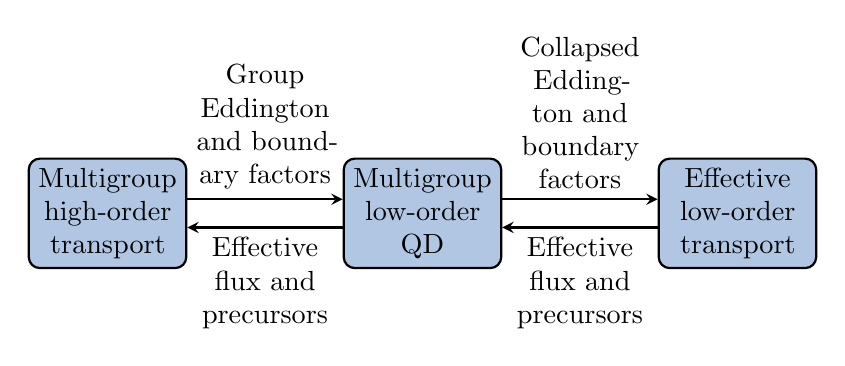
\begin{tikzpicture}
      \node (1) [solver2] {Multigroup high-order transport};
      \node (2) [solver2, right of=1, xshift=3cm] {Multigroup low-order QD};
      \node (3) [solver2, right of=2, xshift=3cm] {Effective low-order transport};
      \draw [arrow] (1.10) -- node[anchor=south, text width=2cm, align=center] {Group\\ Eddington
        and boundary factors} (2.170);
      \draw [arrow] (2.190) -- node[anchor=north, text width=2cm, align=center] {Effective flux
        and precursors} (1.350);
      \draw [arrow] (2.10) -- node[anchor=south, text width=2cm, align=center] {Collapsed Eddington
        and boundary factors} (3.170);
      \draw [arrow] (3.190) -- node[anchor=north, text width=2cm, align=center] {Effective flux
        and precursors} (2.350);
    \end{tikzpicture}
    \caption{Algorithm flowchart for the three-level quasi-diffusion method.}
    \label{fig:algorithm}
  \end{figure}
\end{frame}

\begin{frame}
  \frametitle{Multilevel Quasi-Diffusion Method}
  Tamang \& Anistratov applied the QD method to 1-D time-dependent multiphysics neutron transport
  and heat transfer problems by iteratively coupling the one-group low-order equations to the heat
  transfer and precursor equations \cite{tamang_multilevel_2014}.
  \vspace{.2cm}

  Reynolds \& Palmer applied the same approach for steady-state simulations of a 2-D axisymmetric,
  two-group MSRE model \cite{reynolds_analysis_2023}.
  %
  \begin{figure}[h]
    \centering
    \includegraphics[width=.6\columnwidth]{images/reynolds-flux}
    \caption{Fast and thermal fluxes of the 2-D axisymmetric MSRE model by Reynolds \& Palmer
    \cite{reynolds_analysis_2023}.}
    \label{fig:reynolds-flux}
  \end{figure}
  \textbf{Limitation: Computational expensive for 3-D full-core simulations.}
\end{frame}

\begin{frame}
  \frametitle{Multischeme Transport Method}
  Implemented in the Griffin reactor physics application \cite{wang_hybrid_2017}. This method
  involves making predetermined
  domain decompositions to be treated with the $S_N$, $P_N$, or diffusion methods. Adjoining
  subdomains are coupled through the Lagrange multiplier interface condition:
  \begin{gather}
    -\int_S \left[\left(\llbracket\Psi\rrbracket,\Lambda^*\right)_{\Gamma} +
    \left(\llbracket\Psi^*\rrbracket,\Lambda\right)_{\Gamma}\right] d\hat{\Omega}
    \shortintertext{where}
    \begin{align}
      \llbracket\Psi\rrbracket &= \Psi^+ - \Psi^-, 
      \Psi^\pm = \lim_{s\rightarrow 0^+} \Psi(\vec{x}+s\hat{n}), \nonumber \\
      \Lambda &= \mbox{ Lagrange multiplier},
      \Gamma = \mbox{ interface boundary}, \nonumber \\
      \hat{n} &= \mbox{ normal vector at interface boundary}, \nonumber
    \end{align}
  \end{gather}
  or the upwinding method:
  \begin{gather}
    \int_S \left(|\hat{\Omega}\cdot\hat{n}|\llbracket\Psi^*\rrbracket,\Psi^-\right)_{\Gamma^+}
    d\hat{\Omega} -
    \int_S\left(|\hat{\Omega}\cdot\hat{n}|\llbracket\Psi^*\rrbracket,\Psi^+\right)_{\Gamma^-}
    d\hat{\Omega}
  \end{gather}
\end{frame}

\begin{frame}
  \frametitle{Hybrid Transport-Diffusion Method \cite{anistratov_computational_2012, stehle_hybrid_2014}}
  \vspace{.2cm}

  Anistratov \& Stehle developed an adaptive domain decomposition scheme using Eddington tensor
  estimates as a metric for deducing whether a region is diffusive or
  transport-like.
  \vspace{.2cm}

  It uses two-level neutronics method based on the Second-Moment method \cite{lewis_comparison_1976}.
  The low-order second-moment equations on the $(s+1)$th iteration are:
  \begin{gather}
    \nabla\cdot J^{(s+1)}+\Sigma_a\phi^{(s+1)} = q, \label{eq:2nd-moment-1} \\
    \frac{1}{3}\nabla\cdot\phi^{(s+1)}+\Sigma_t J^{(s+1)} = \nabla\cdot F^{(s+1/2)}
    \label{eq:2nd-moment-2}
    \shortintertext{where}
    F^{(s+1/2)}_{\alpha\beta} = \int_{4\pi}
    \left(\frac{1}{3}\delta_{\alpha\beta}-\Omega_\alpha\Omega_\beta\right)
    \Psi^{(s+1/2)} d\Omega \label{eq:2nd-moment-3}
  \end{gather}
  %
  The transport subdomains require interface conditions in the form of boundary sources from
  neighboring diffusion subdomains.

  \textbf{Limitation: Complicated implementation and management of computational resources.}
\end{frame}

\begin{frame}
  \frametitle{Hybrid $S_N$-Diffusion Method: Literature Review}
  \begin{block}{\textbf{Summary}}
    \begin{itemize}
      \item Corrective terms for the neutron diffusion equations in various forms have been
        effectively applied across various methods.
      \item Domain decomposition is necessary for limiting computational cost in large 3-D reactor
        simulations.
      \item Interface conditions are required when applying domain decomposition to iteratively
        couple the transport and diffusion solvers.
%      \item Demonstrations of the Ronen method are limited to 1-D geometries due to the difficulty of
%        deriving transport operators for complex 2-D and 3-D geometries
    \end{itemize}
  \end{block}
\end{frame}

\subsection{Theory}
\begin{frame}
  \frametitle{Hybrid $S_N$-Diffusion Method: Theory}
  \textbf{Hybrid $\bm{S_N}$-Diffusion Method}
%  \begin{block}{\textbf{Aim}}
%    To enable accurate control rod modeling in time-dependent molten salt reactor simulations
%  \end{block}
  \begin{block}{\textbf{Method Overview}}
    \begin{itemize}
      \item Applies the discrete ordinates ($S_N$) method to a small subregion around a
        control rod to generate corrections for the neutron diffusion equation
      \item Limits computationally expensive $S_N$ calculations to small subdomains
      \item Retains the computational efficiency of the neutron diffusion method
      \item Applies an adaptive algorithm to smooth flux gradients near the $S_N$-diffusion interface
    \end{itemize}
  \end{block}
  \begin{figure}
    \centering
    \includegraphics[width=.7\textwidth]{hybrid-illustration}
    \caption{Illustration of the problem domains of the $S_N$ and neutron diffusion methods in an
    example 1-D problem.}
  \end{figure}
\end{frame}

\begin{frame}
  \frametitle{Hybrid $S_N$-Diffusion Method: Theory}
  \textbf{Multigroup Discrete Ordinates $\bm{S_N}$ Neutron Transport Equations}
  \vspace{.2cm}

  The multigroup $S_N$ equations defined on the 3-D spatial domain 
  $\mathcal{D}$ and 2-D unit sphere angular domain $\mathcal{S}$ is:
  \begin{multline}
    \hat{\Omega}\cdot\nabla\Psi_g(\vec{r},\hat{\Omega},t) + \Sigma_{t,g}
    \Psi_g(\vec{r},\hat{\Omega},t) =
    \sum^G_{g'=1}\int_\mathcal{S} \Sigma_s^{g'\rightarrow g}(\hat{\Omega}'\rightarrow\hat{\Omega})
    \Psi_{g'}(\vec{r},\hat{\Omega}',t)d\hat{\Omega}' \\
    + \frac{1}{4\pi}\frac{\chi_{p,g}(1-\beta)}{k}\sum^G_{g'=1} \nu\Sigma_{f,g'} \phi_{g'}(\vec{r},t)
    + \frac{1}{4\pi}\sum^I_{i=1}\chi_{d,g}
    \lambda_i C_i(\vec{r},t)
    \label{eq:mg-nte}
  \end{multline}
  with boundary conditions:
  %
  \begin{gather}
    \Psi_g(\vec{r},\hat{\Omega}) = \Psi^\text{inc}_g(\vec{r},\hat{\Omega}) +
    \alpha^s_g\Psi_g(\vec{r},\hat{\Omega}_r)
    \mbox{ on } \vec{r} \in \partial\mathcal{D} \mbox{ and } \hat{\Omega}\cdot\hat{n}_b < 0,
    \shortintertext{where}
    \begin{align*}
%      \chi_{p,g} &= \mbox{prompt fission neutron spectrum in group $g$,} \\
%      \beta &= \sum^I_{i=1} \beta_i = \mbox{total delayed neutron fraction,} \\
%      \chi_{d,g} &= \mbox{delayed fission neutron spectrum in group $g$,} \\
%      \lambda_i &= \mbox{decay constant of precursor group $i$,} \\
%      C_i &= \mbox{delayed neutron precursor concentration for group $i$,} \\
      \Psi^\text{inc}_g &= \mbox{incident surface source in group $g$,} \\
      \alpha^s_g &= \mbox{specular reflectivity on }\partial \mathcal{D} \mbox{ for group }g, \\
      \hat{\Omega}_r &= \hat{\Omega}-2(\hat{\Omega}\cdot \hat{n}_b)\hat{n}_b = \mbox{reflection angle}, \\
      \hat{n}_b &= \mbox{outward unit normal vector on the boundary.}
    \end{align*}
  \end{gather}
\end{frame}

\begin{frame}
  \frametitle{Hybrid $S_N$-Diffusion Method: Theory}
  \textbf{Self-Adjoint Angular Flux (SAAF) Formulation of the Multigroup $\bm{S_N}$ Equations}
  \vspace{.2cm}

  Second-order linear neutron transport equation derived by obtaining the analytical solution of
  angular flux and substituting it back into the $S_N$ equations.

  \begin{block}{\textbf{Implementation Details}}
    \begin{itemize}
      \item Implemented with finite element method (FEM)
      \item Compatible with the efficient and scalable Hypre-BoomerAMG preconditioning
      \item Uses a modified formulation to handle $1/\Sigma_{t,g}$ factor in void regions (similar to
        Streamline-Upwind/Petrov Galerkin (SUPG) stabilization scheme) \cite{wang_diffusion_2014}
      \item Level-symmetric quadrature set for angular discretization (up to $S_{18}$)
      \item Nonlinear diffusion acceleration scheme \cite{wang_diffusion_2014}
    \end{itemize}
  \end{block}
\end{frame}

\begin{frame}
  \frametitle{Hybrid $S_N$-Diffusion Method: Theory}
  \textbf{Weak Formulation of the Multigroup SAAF $S_N$ Equations}
  \begin{gather}
    \shortintertext{Streaming term:}
    \sum^G_{g=1}\sum^{N_d}_{d=1}w_d\left(\hat{\Omega}_d\cdot\nabla\Psi^*_{g,d},\tau_g\hat{\Omega}
    \cdot\nabla\Psi_{g,d}-(1-\tau_g\Sigma_{t,g})\Psi_{g,d}\right)_\mathcal{D} \\
    \shortintertext{Collision term: }
    \sum^G_{g=1}\sum^{N_d}_{d=1}w_d\left(\Psi^*_{g,d},\Sigma_{t,g}\Psi_{g,d}\right)_\mathcal{D} \\
    \shortintertext{Scattering term:}
    \sum^G_{g=1}\sum^{N_d}_{d=1}w_d\left(\Psi^*_{g,d}+\tau_g\hat{\Omega}_d\cdot\nabla\Psi^*_{g,d},
    \sum^G_{g'=1}\sum^L_{l=0}\Sigma^{g'\rightarrow g}_{s,l}\sum^l_{m=-l}
    \frac{2l+1}{w}Y_{l,m}(\hat{\Omega}_d)\phi_{g',l,m}\right)_\mathcal{D} \\
    \shortintertext{Fission source term: }
    \sum^G_{g=1}\sum^{N_d}_{d=1}w_d\left(\Psi^*_{g,d}+\tau_g\hat{\Omega}_d\cdot\nabla\Psi^*_{g,d},
    \frac{1}{w}\frac{\chi_{p,g}(1-\beta)}{k}\sum^G_{g'=1}\nu\Sigma_{f,g'}\phi_{g'}\right)_\mathcal{D}
  \end{gather}
\end{frame}

\begin{frame}
  \frametitle{Hybrid $S_N$-Diffusion Method: Theory}
  \textbf{Weak Formulation of the Multigroup SAAF $S_N$ Equations}
  \begin{gather}
    \shortintertext{Delayed neutron source term:}
    \sum^G_{g=1}\sum^{N_d}_{d=1}w_d\left(\Psi^*_{g,d}+\tau_g\hat{\Omega}_d\cdot\nabla\Psi^*_{g,d},
    \frac{1}{w}\sum ^I_{i=1}\chi_{d,g}\lambda_i C_i\right)_\mathcal{D}
    \shortintertext{Boundary source term:}
    \begin{cases}
      \sum^G_{g=1}\sum^{N_d}_{d=1}w_d\left(\Psi^*_{g,d},
      \hat{\Omega}_d\cdot\hat{n}_b\Psi_{g,d}\right)_{\partial\mathcal{D}},
      & \hat{\Omega}\cdot\hat{n}_b>0,\vec{r}\in\partial\mathcal{D} \\
      \sum^G_{g=1}\sum^{N_d}_{d=1}w_d\left(\Psi^*_{g,d},
      \hat{\Omega}_d\cdot\hat{n}_b\Psi^\text{inc}_{g,d}\right)_{\partial\mathcal{D}},
      & \hat{\Omega}\cdot\hat{n}_b<0,\vec{r}\in\partial\mathcal{D}
    \end{cases} \label{eq:boundary-source} \\
    \shortintertext{Reflecting boundary term:}
    \begin{cases}
      \sum^G_{g=1}\sum^{N_d}_{d=1}w_d\left(\Psi^*_{g,d},
      \hat{\Omega}_d\cdot\hat{n}_b\Psi_{g,d}\right)_{\partial\mathcal{D}},
      & \hat{\Omega}\cdot\hat{n}_b>0,\vec{r}\in\partial\mathcal{D}_s \\
      \sum^G_{g=1}\sum^{N_d}_{d=1}w_d\left(\Psi^*_{g,d},
      \hat{\Omega}_d\cdot\hat{n}_b\Psi_{g,d_r}\right)_{\partial\mathcal{D}},
      & \hat{\Omega}\cdot\hat{n}_b<0,\vec{r}\in\partial\mathcal{D}_s
    \end{cases} \label{eq:reflecting-bc}
  \end{gather}
\end{frame}

\begin{frame}
  \frametitle{Hybrid $S_N$-Diffusion Method: Theory}
  \textbf{Weak Formulation of the Multigroup SAAF $S_N$ Equations}
  \begin{gather}
    \shortintertext{Void stabilization parameter \cite{wang_diffusion_2014}:}
    \tau_g =
    \begin{cases}
      \frac{1}{c\Sigma_{t,g}} \mbox{ for } ch\Sigma_{t,g} \geq \varsigma \\
      \frac{h}{\varsigma} \mbox{ for } ch\Sigma_{t,g} < \varsigma
    \end{cases}, \\
    \shortintertext{where}
    \begin{align*}
      h &= \mbox{mesh element size,} & \\
      c &= \mbox{maximum stabilization factor,} & \\
      \varsigma &= \mbox{void constant.} &
    \end{align*}
  \end{gather}
  $c=1$ and $\varsigma=0.5$ by default.
  \vspace{.2cm}

  The SAAF-$S_N$ equations require this stabilization scheme
  in near-void regions where $\Sigma_{t,g}$ is very small.
\end{frame}

\begin{frame}
  \frametitle{Hybrid $S_N$-Diffusion Method: Theory}
  \textbf{Multigroup Neutron Diffusion Equations}
  \begin{gather}
    - \nabla \cdot D_g \nabla \phi_g + \Sigma^r_g \phi_g =
    \sum^G_{g' \neq g} \Sigma^s_{g' \rightarrow g} \phi_{g'}
    + \frac{\chi_{p,g} \left( 1-\beta \right)}{k} \sum^G_{g'=1} \nu \Sigma^f_{g'}
    \phi_{g'} + \chi^d_g \sum^I_i \lambda_i C_i \label{eq:neutron} %\\
  \end{gather}
  %
  Traditionally, $D_g$ is determined through region-wide neutron interaction tallies in
  high-fidelity neutron transport simulations as follows:
  \begin{align}
    D_g =& \frac{1}{3\Sigma_{t,g}} \quad \mbox{(isotropic)} \\
    D_g =& \frac{1}{3\Sigma_{tr,g}} = \frac{1}{3\left(\Sigma_{t,g}-
    \Sigma_{s1,g}\right)}
    \quad \mbox{(linearly anisotropic)} \label{eq:p1-diffcoef}
    \shortintertext{where}
    \Sigma_{tr} =& \mbox{ macroscopic transport cross section} \nonumber
  \end{align}
\end{frame}

\begin{frame}
  \frametitle{Hybrid $S_N$-Diffusion Method: Theory}
  \textbf{Diffusion Correction Scheme (Implemented in Python)}
  \vspace{.2cm}

  In this work, I investigated two transport correction schemes. The first scheme is the diffusion
  correction scheme similar to Fick's first law of diffusion:
  \begin{gather}
    D^s_g(x) = -J^{tr}_g(x)\bigg/\frac{d\phi^{tr}_g(x)}{dx} \label{eq:svdc}
  \end{gather}
  %
  where $D^s_g$ is the diffusion correction parameter, and the $tr$ superscript denotes the
  transport-derived neutron current and scalar flux solutions from the $S_N$ method.
  \vspace{.2cm}

%  $D^s_g$ provides pointwise corrections to closely match the diffusion flux solution to the $S_N$
%  flux solution.
  By replacing $D_g$ with $D^s_g$, we are effectively adding the following transport correction term
  %
  \begin{gather}
    -\nabla\cdot (D^s_g-D_g)\nabla\phi_g
  \end{gather}
  to the neutron diffusion equations.
  \vspace{.2cm}

  $\Rightarrow$ Abandoned after 1-D investigations due to division-by-zero issues near flux maximas
  and minimas.
\end{frame}

\begin{frame}
  \frametitle{Hybrid $S_N$-Diffusion Method: Theory}
  \textbf{Drift Correction Scheme (Implemented on Moltres)}
  \vspace{.2cm}

  The second scheme is the drift correction scheme arising from adding a drift term
  ($\vec{D}_g\cdot\nabla \phi_g$) to the neutron diffusion equations:
  \begin{gather}
  \scalebox{0.95}{$
    \vec{D}_g = \frac{\sum^{N_d}_{d=1}w_d\left(\tau_g\hat{\Omega}_d\hat{\Omega}_d\cdot\nabla\Psi_{g,d}
    + \left(\tau_g\Sigma_{t,g}-1\right)\hat{\Omega}_d\Psi_{g,d}
    - \tau_g\sum^G_{g'=1}\Sigma^{g'\rightarrow g}_{s,1}\hat{\Omega}_d\Psi_{g',d}
- D_g\nabla\Psi_{g,d}\right)}{\sum^{N_d}_{d=1}w_d\Psi_{g,d}},$} \label{eq:drift} \\
  \scalebox{0.95}{$
    \gamma_g =
    \frac{\sum_{\hat{\Omega}_d\cdot\hat{n}_b > 0}w_d |\hat{\Omega}_d\cdot\hat{n}_b |
  \Psi_{g,d}}{\sum^{N_d}_{d=1}w_d\Psi_{g,d}}.$} \label{eq:bound-coef}
  \end{gather}
  \vspace{.2cm}

  The drift term also provides pointwise corrections to the neutron diffusion equations. This
  formulation is derived from the SAAF-$S_N$ equations by integrating over the angular domain and
  eliminating terms shared by the neutron diffusion equations.
\end{frame}

\begin{frame}
  \frametitle{Hybrid $S_N$-Diffusion Method: Theory}
  \textbf{$S_N$ Subsolver Boundary Conditions}
  \vspace{.2cm}

  For the hybrid $S_N$-diffusion method to converge, it requires appropriate boundary conditions for
  the $S_N$ subproblem.
  We may obtain
  the best estimate by applying the $P_1$ approximation for evaluating the neutron angular flux along
  the discrete ordinates $\hat{\Omega}_d$ of the $S_N$ angular quadrature set as follows:
  \begin{align}
    \Psi_{g,d} &\approx \frac{1}{4\pi}\left(\phi^\text{diff}_g+3\hat{\Omega}_d\cdot
    \vec{J}^\text{diff}_g\right) \nonumber \\
    &=\frac{1}{4\pi}\left(\phi^\text{diff}_g-3\hat{\Omega}_d\cdot D_g\nabla\phi^\text{diff}_g\right)
  \end{align}
  Therefore, the boundary source term for the $S_N$ subsolver is:
  \begin{gather}
    \Psi^\text{inc}_{g,d} = \frac{1}{w}
    \left(\phi^\text{diff}_g-3\hat{\Omega}_d\cdot D_g\nabla\phi^\text{diff}_g\right)
  \end{gather}
  where $w$ is the sum of weights of the level-symmetric quadrature set.
\end{frame}

\begin{frame}
  \frametitle{Hybrid $S_N$-Diffusion Method: Theory}
  \begin{columns}
    \column{.35\textwidth}
    \textbf{Hybrid $S_N$-Diffusion Method Algorithm}
    \vspace{.5cm}

  {\small
  $V_0$: Full problem domain
  \vspace{.1cm}

  $V_1$: Problem subdomain containing control rod region
  \vspace{.1cm}

  $D^{s,(i)}_g$: diffusion correction parameter in the $i$-th iteration
  \vspace{.1cm}

  $\vec{D}^{(i)}_g$: drift correction parameter in the $i$-th iteration
\vspace{4cm}}
  \column{.65\textwidth}
  \begin{figure}
    \centering
    \includegraphics[width=.46\textwidth]{images/algorithm}
    \begin{minipage}[b]{.49\textwidth}
      \caption{Algorithm flowchart for the hybrid $S_N$-diffusion method.}
    \end{minipage}
  \end{figure}
\end{columns}
\end{frame}

\begin{frame}
  \frametitle{Hybrid $S_N$-Diffusion Method: Theory}
  \textbf{Correction Region ($\bm{V_1}$) and Buffer Zone}
  \begin{itemize}
    \item Recall that the full problem domain and the correction region are defined as $V_0$
      and $V_1$, where $V_1 \subseteq V_0$
    \item The approximate $S_N$ boundary conditions will generally yield some deviations in the
      flux distribution since neutron fluxes in realistic reactor systems are at least slightly
      anisotropic throughout most of the system
    \item However, the influence of boundary conditions on the ratio of $J$ and $\frac{d\phi}{dx}$
      does not extend far from the boundary $\partial V_1$ in optically thick media; transport
      correction parameters are accurate everywhere except near $\partial V_1$
    \item There exists a buffer zone near $\partial V_1$ where transport correction parameters
      are inaccurate
  \end{itemize}
%  \pause
%  $\Rightarrow$ Approach for preliminary results: Define $V_1$ such that it is large enough to
%  provide sufficient transport
%  corrections and accommodate inaccurate SVDCs near $\partial V_1$. Discard inaccurate SVDCs
%  in favor of the default $P_1$-based diffusion coefficients.
\end{frame}

\begin{frame}
  \frametitle{Hybrid $S_N$-Diffusion Method: Theory}
  \textbf{Correction Region ($\bm{V_1}$) and Buffer Zone}
  \begin{figure}[htb!]
    \centering
    \includegraphics[width=.5\columnwidth]{case-3b-geometry}
    \caption{1-D geometry for Case 3b.}
    \label{fig:3b-geometry}
  \end{figure}
  \begin{figure}[htb!]
      \centering
      \begin{subfigure}[t]{.49\textwidth}
          \centering
          \includegraphics[width=.9\textwidth]{case-3b-group-1-drift}
      \end{subfigure}
      \hfill
      \begin{subfigure}[t]{.49\textwidth}
          \centering
          \includegraphics[width=.9\textwidth]{case-3b-group-8-drift}
      \end{subfigure}
      \caption{The reference and hybrid drift ($\vec{D}_g$) distributions for group 1 and 8 calculated
        from $S_8$ and $S_8$-diffusion simulations. The correction subregion $V_1$ spans $x=0$ cm to
        $x=10$ cm.}
      \label{fig:3b-drift-1}
  \end{figure}
\end{frame}

\begin{frame}
  \frametitle{Hybrid $S_N$-Diffusion Method: Theory}
  \textbf{Correction Region ($\bm{V_1}$) and Buffer Zone}
  \vspace{.2cm}

  A natural/intuitive criterion for the location of the buffer zone cutoff boundary
  would be wherever the components of the drift correction variable $\vec{D}_g$ is zero, i.e.,
  wherever the components change signs.
  \begin{enumerate}
    \item At points where the $\vec{D}_g$ components are zero, the flux is approximately isotropic
      along the axes corresponding to the components.
    \item This choice preserves the smoothness of the neutron flux gradient.
  \end{enumerate}
  \begin{figure}[htb!]
      \centering
      \begin{subfigure}[t]{.49\textwidth}
          \centering
          \includegraphics[width=.9\textwidth]{case-3b-group-1-drift}
      \end{subfigure}
      \hfill
      \begin{subfigure}[t]{.49\textwidth}
          \centering
          \includegraphics[width=.9\textwidth]{case-3b-group-8-drift}
      \end{subfigure}
      \caption{The reference and hybrid drift ($\vec{D}_g$) distributions for group 1 and 8 calculated
        from $S_8$ and $S_8$-diffusion simulations. The correction subregion $V_1$ spans $x=0$ cm to
        $x=10$ cm.}
      \label{fig:3b-drift-1}
  \end{figure}
\end{frame}

\begin{frame}
  \frametitle{Hybrid $S_N$-Diffusion Method: Theory}
  \textbf{Numerical Implementation}
  \vspace{.2cm}

  The SAAF-$S_N$ and hybrid $S_N$-diffusion method with the drift correction scheme were
  implemented on Moltres.
  \begin{itemize}
    \item Preconditioned Jacobian-free Newton-Krylov (PJFNK) solver \cite{knoll_jacobian-free_2004}
    \item Hypre-BoomerAMG (Algebraic multigrid) preconditioning \cite{hypre_hypre_2022}
    \item MultiApp and Transfers systems from MOOSE for iterative coupling and data transfers
    \item Supporting material and utility C++ classes for loading group constant data and performing
      angular quadrature calculations
  \end{itemize}
  \vspace{.2cm}

  A 1-D hybrid $S_N$-diffusion method with the diffusion correction
  scheme was implemented in Python. (This scheme was abandoned after 1-D analyses due to division by
  zero errors wherever the flux gradients approach zero.)
  \begin{itemize}
    \item 1-D $S_N$ method with diamond differencing scheme
    \item 1-D neutron diffusion method with finite differencing scheme
  \end{itemize}
\end{frame}

\subsection{Neutronics Eigenvalue Simulations}
\begin{frame}
  \frametitle{1-D MSRE Neutronics Model Geometries}
  \begin{figure}[htb!]
    \centering
    \includegraphics[width=0.9\columnwidth]{case-geometry}
    \caption{Geometries of the 1-D test cases. The material labeled ``mixture'' represents a
      homogeneous mixture of fuel and graphite at a ratio of 22.5\%-77.5\% by volume. All geometries
      have reflective boundary conditions on the boundary at $x=0$ cm. The right-side boundaries are
      reflective for Cases 1a and 1b, and vacuum for Cases 2a, 2b, 3a, and 3b.}
    \label{fig:case-geom}
  \end{figure}
\end{frame}

\begin{frame}
  \frametitle{1-D MSRE Neutronics Modeling Approach}
  \begin{columns}
    \column{5.5cm}
    \textbf{1-D Neutronics Model Setup}
    \vspace{.2cm}

    \begin{itemize}
      \item Material compositions derived from the MSRE design
      \item Reduced gadolinium content in control rod to 0.35 wt\%
      \item Eight neutron energy groups
      \item Group constants generated using OpenMC with up to 2nd-order Legendre expansions of scattering
        matrices
      \item Uniform temperature at 900 K
    \end{itemize}
    \column{5.5cm}
    \begin{table}[h]
      \centering
      \caption{Neutron energy group structure in this work. Originally devised by Jaradat
      \cite{jaradat_development_2021-1}.}
      \begin{tabular}{r S}
        \toprule
        Group & {Upper energy bound [eV]} \\
        \midrule
        1 & 2.000$\times 10^7$ \\
        2 & 1.353$\times 10^6$ \\
        3 & 6.734$\times 10^4$ \\
        4 & 9.118$\times 10^3$ \\
        5 & 1.487$\times 10^2$ \\
        6 & 4.000$\times 10^0$ \\
        7 & 6.250$\times 10^{-1}$ \\
        8 & 8.000$\times 10^{-2}$ \\
        \bottomrule
      \end{tabular}
      \label{table:energy-group}
    \end{table}
  \end{columns}
\end{frame}

\begin{frame}
  \frametitle{1-D MSRE Neutronics Modeling Approach}
  \textbf{1-D Neutronics Model Numerical Solvers}
  \vspace{.2cm}

  All 1-D cases ran on each of the following numerical solvers:
  \begin{enumerate}
    \item OpenMC in continuous energy mode (OpenMC-CE)
    \item OpenMC in multigroup mode (OpenMC-MG)
    \item Neutron diffusion method (Moltres \& Python)
    \item $S_8$ method (Moltres \& Python)
    \item Hybrid $S_8$-diffusion method (Moltres \& Python)
  \end{enumerate}
  \vspace{.2cm}

  \textbf{Reactivity \& Reactivity Difference}
  \begin{gather}
    \mbox{Reactivity } \rho \equiv \frac{k_\text{eff}-1}{k_\text{eff}}.
  \end{gather}
  \begin{gather}
    \Delta\rho = \rho_1 - \rho_2 =
    \frac{k_{\text{eff},1}-k_{\text{eff},2}}{k_{\text{eff},1}k_{\text{eff},2}}.
  \end{gather}
\end{frame}

\begin{frame}
  \frametitle{1-D MSRE Neutronics Simulation Results}
  \textbf{1-D Neutronics Model Reactivity Results}
  \begin{figure}[h]
    \centering
    \includegraphics[width=\columnwidth]{rho}
    \caption{Difference in reactivity $\rho$ of all neutronics methods investigated relative
    to OpenMC-CE.}
    \label{fig:1d-rho}
  \end{figure}
\end{frame}

\begin{frame}
  \frametitle{1-D MSRE Neutronics Simulation Results}
  \textbf{1-D Neutronics Model Control Rod Worth Results}
  \begin{figure}[h]
    \centering
    \includegraphics[width=\columnwidth]{worth}
    \caption{Percentage difference in rod worth for Cases 2 and 3 of all neutronics methods
    investigated relative to OpenMC-CE.}
    \label{fig:1d-worth}
  \end{figure}
\end{frame}

\begin{frame}
  \frametitle{1-D MSRE Neutronics Simulation Results}
  \textbf{Case 3b Geometry}
  \begin{figure}
    \centering
    \includegraphics[width=.7\textwidth]{hybrid-illustration}
    \caption{Geometry of 1-D Case 3b.}
  \end{figure}
\end{frame}

\begin{frame}
  \frametitle{1-D MSRE Neutronics Simulation Results}
  \textbf{Case 3b Neutron Flux Distributions}
  \begin{figure}[htb!]
    \centering
    \includegraphics[width=.75\columnwidth]{images/case-3b-flux-diff-pres}
    \caption{Absolute difference in neutron group flux distributions for Case 3b from Moltres-$S_8$,
    Moltres-diffusion, and Moltres-hybrid relative to OpenMC-MG.}
    \label{fig:3b-flux-diff}
  \end{figure}
%  \begin{itemize}
%    \item The neutron diffusion and hybrid methods fare worse than the $S_8$ method at capturing
%      the oscillatory flux pattern.
    The hybrid method provides more accurate flux estimates than the neutron diffusion method near $x=0$ cm where
      the control rod is situated.
%  \end{itemize}
\end{frame}

%\begin{frame}
%%  \frametitle{Hybrid $S_N$-Diffusion Method: 1-D Neutronics Eigenvalue Simulations}
%  \begin{columns}
%    \column{5.5cm}
%    \textbf{Case 3b Neutron Flux Distributions}
%    \begin{itemize}
%      \item The neutron diffusion and hybrid methods fare worse than the $S_8$ method at capturing
%        the oscillatory flux pattern.
%      \item The hybrid method performs better than the neutron diffusion method near $x=0$ cm where
%        the control rod is situated.
%    \end{itemize}
%    \column{5.5cm}
%    \begin{figure}[htb!]
%      \centering
%      \includegraphics[width=.975\columnwidth]{case-3b-flux-diff}
%      \caption{Absolute difference in neutron group flux distributions for Case 3b from Moltres-$S_8$,
%      Moltres-diffusion, Moltres-hybrid, and Python-hybrid relative to OpenMC-MG.}
%      \label{fig:3b-flux-diff}
%    \end{figure}
%  \end{columns}
%\end{frame}

\begin{frame}
  \frametitle{1-D MSRE Neutronics Simulation Results}
  \textbf{Impact of Correction Subregion Sizes on Rod Worth}
  \begin{itemize}
    \item Rod worth estimates vary non-monotonically with increasing correction subregion size.
    \item Rod worth estimates remain within 0.2\% of the $S_8$ method rod worth.
    \item The hybrid method produces accurate rod worth estimates as long as the correction region
      size is kept consistent.
  \end{itemize}
  \begin{figure}[htb!]
    \centering
    \includegraphics[width=0.6\columnwidth]{correction-size-rho}
    \caption{Percentage difference in rod worth from the hybrid method relative to OpenMC-CE for
      Cases 3a and 3b with different correction subregion sizes.}
    \label{fig:v1-size-rho}
  \end{figure}
\end{frame}

\begin{frame}
  \frametitle{1-D MSRE Neutronics Simulation Results}
  \begin{columns}
    \column{6.5cm}
    \textbf{Relaxing the $S_N$ Convergence Tolerance,} $\bm{\epsilon}_\text{tol}$
    \begin{itemize}
      \item Transport correction parameters converge faster than scalar flux in the $S_N$ subsolver.
      \item Relaxing the $S_N$ subsolver convergence tolerance would provide computational savings.
      \item The hybrid method exhibits superlinear ($q=1.333$) convergence in $k$ with respect to
        the $S_8$ convergence tolerance value.
    \end{itemize}
    \begin{table}[h]
      \centering
      \caption{Number of outer iterations in hybrid method calculations of Case 3b for a given set of
      convergence tolerance values imposed on the $S_8$ subsolver.}
      \small
      \setlength\tabcolsep{2pt}
      \begin{tabular}{l S S S S S S}
        \toprule
        Tolerance value, $\epsilon_\text{tol}$ & {$10^{-8}$} & {$10^{-7}$} & {$10^{-6}$} & {$10^{-5}$} & {$10^{-4}$} & {$10^{-3}$} \\
        \midrule
        No.\ of outer iterations & 3 & 3 & 3 & 2 & 2 & 1 \\
        \bottomrule
      \end{tabular}
      \label{table:sn-tol}
    \end{table}
    \column{4.5cm}
    \begin{figure}[h]
      \centering
      \includegraphics[width=\columnwidth]{sn-tol}
      \caption{$k_\text{eff}$ error estimates of Case 3b for a range of $S_8$ subsolver convergence tolerance values
      relative to the reference $k_\text{eff}$ value when
      $\epsilon_\text{tol}=10^{-8}$.}
      \label{fig:sn-tol}
    \end{figure}
  \end{columns}
\end{frame}

\begin{frame}
  \frametitle{Hybrid $S_N$-Diffusion Method: 2-D Neutronics Eigenvalue Simulations}
  \textbf{2-D Neutronics Quarter-Core \& Full-Core MSRE Models}
  \begin{columns}
    \column{5.5cm}
  \begin{figure}[htb!]
    \centering
    \includegraphics[width=\columnwidth]{quarter-core-geom}
    \caption{2-D \gls{MSRE} quarter-core model based on the horizontal cross section of the actual
    \gls{MSRE} geometry.}
    \label{fig:1/4-geom}
  \end{figure}
  \column{5.5cm}
  \begin{figure}[htb!]
    \centering
    \includegraphics[width=\columnwidth]{full-core-geom}
    \caption{2-D \gls{MSRE} full-core model based on the horizontal cross section of the actual
    \gls{MSRE} geometry.}
    \label{fig:full-geom}
  \end{figure}
\end{columns}
\end{frame}

\begin{frame}
  \frametitle{Hybrid $S_N$-Diffusion Method: 2-D Neutronics Eigenvalue Simulations}
  \begin{columns}
    \column{6.5cm}
    \textbf{2-D Neutronics MSRE Model Setup}
    \vspace{.2cm}

    Geometry approximations:
    \begin{itemize}
      \item Modeled the control rods as perfectly annular cylinders
      \item Homogenized the nickel alloy, graphite, and molten salt regions in the sample basket
      \item Neglected the thermal insulation and shield structures outside the core
      \item Replaced partial fuel channels and jagged graphite edges on the core periphery
    \end{itemize}
    All material compositions correspond to the original MSRE specifications at initial criticality.
    \column{4.5cm}
    \begin{figure}[htb!]
      \centering
      \includegraphics[width=\columnwidth]{full-core-closeup}
      \caption{Detailed view of the control rod thimbles and sample basket in 2-D \gls{MSRE} full-core
        model.}
      \label{fig:full-geom-closeup}
    \end{figure}
  \end{columns}
\end{frame}

\begin{frame}
  \frametitle{Hybrid $S_N$-Diffusion Method: 2-D Neutronics Eigenvalue Simulations}
  \textbf{2-D Quarter-Core $k$ \& Rod Worth Results}
  \begin{table}[htb]
    \small
    \centering
    \caption{$k_\text{eff}$ and control rod worth estimates for the 2-D quarter-core \gls{MSRE}
      model. Error values are relative to OpenMC-CE.}
    \setlength\tabcolsep{2pt}
    \begin{tabular}{l S[table-format=1.5(2)] S S[table-format=1.5(2)] S S[table-format=4(2)] S}
      \toprule
      \multirow{2}{*}{Method} & \multicolumn{2}{c}{No Rod} & \multicolumn{2}{c}{Rod} & \multicolumn{2}{c}{Rod worth} \\
                              & {$k_\text{eff}$} & {Error [pcm]} & {$k_\text{eff}$} & {Error [pcm]} & {$\Delta\rho_\text{worth}$ [pcm]} & {Error [pcm]} \\
                              \cmidrule(r){1-1} \cmidrule(rl){2-3} \cmidrule(rl){4-5} \cmidrule(l){6-7}
  	  OpenMC-CE & 1.11209(43) & {-} & 1.01740(42) & {-} & 8370(53) & {-} \\
  	  OpenMC-MG & 1.11979(42) & 618 & 1.02204(41) & 446 & 8541(51) & 172 \\
        Diffusion & 1.12059 & 682 & 1.00903 & -816 & 9867 & 1484 \\
        Hybrid & 1.12174 & 773 & 1.02532 & 760 & 8383 & 13 \\
      \bottomrule
    \end{tabular}
    \label{table:quarter-core}
  \end{table}
  \vspace{.2cm}

  The hybrid method produces accurate rod worth estimates while the neutron diffusion method
      significantly overestimates rod worth.
\end{frame}

\begin{frame}
%  \frametitle{Hybrid $S_N$-Diffusion Method: 2-D Neutronics Eigenvalue Simulations}
%  \textbf{Normalized Fuel Channel Power Distribution}
  \begin{columns}
    \column{6cm}
    \centerline{\textbf{Control Rod Withdrawn}}
  \begin{figure}[p]
    \centering
    \includegraphics[width=\columnwidth]{msre-quarter-no-rod-power}
    \caption{Normalized channel fission rate distribution of the 2-D \gls{MSRE} quarter-core model
    with the rod withdrawn.}
    \label{fig:1/4-no-rod}
  \end{figure}
    \column{6cm}
    \centerline{\textbf{Control Rod Inserted}}
  \begin{figure}[p]
    \centering
    \includegraphics[width=\columnwidth]{msre-quarter-rod-power}
    \caption{Normalized channel fission rate distribution of the 2-D \gls{MSRE} quarter-core model
    with the rod inserted.}
    \label{fig:1/4-rod}
  \end{figure}
\end{columns}
\end{frame}

\begin{frame}
  \frametitle{Hybrid $S_N$-Diffusion Method: 2-D Neutronics Eigenvalue Simulations}
  \textbf{2-D Quarter-Core Normalized Fuel Channel Power Distribution}
  \begin{table}[htb]
    \small
    \centering
    \caption{Absolute mean and maximum percentage errors in the normalized channel fission rates of
    the 2-D \gls{MSRE} quarter-core models relative to OpenMC. The mean relative standard deviation of
    OpenMC normalized channel fission rates is 0.20\%.}
    \begin{tabular}{l S S S S}
      \toprule
      \multirow{2}{*}{Method} & \multicolumn{2}{c}{No Rod} & \multicolumn{2}{c}{Rod} \\
                              & {Mean [\%]} & {Maximum [\%]} & {Mean [\%]} & {Maximum [\%]} \\
                              \cmidrule(r){1-1} \cmidrule(rl){2-3} \cmidrule(l){4-5}
      Diffusion & 0.40 & 2.63 & 2.01 & 17.44 \\
      Hybrid & 0.40 & 1.32 & 0.43 & 3.08 \\
      \bottomrule
    \end{tabular}
    \label{table:quarter-core-power}
  \end{table}
  \vspace{.2cm}

  \begin{itemize}
    \item The hybrid method improves channel fission rate estimates, especially for the rodded case.
    \item Significant improvement in maximum percentage error of the channel fission rate.
  \end{itemize}
\end{frame}

\begin{frame}
  \frametitle{Hybrid $S_N$-Diffusion Method: 2-D Neutronics Eigenvalue Simulations}
  \textbf{2-D Full-Core Rod Worth Results}
  \begin{table}[htb]
    \small
    \centering
    \caption{Control rod worth estimates for the 2-D full-core \gls{MSRE} with the
    indicated rods inserted. Error values are relative to OpenMC-CE.}
    \setlength\tabcolsep{2pt}
    \begin{tabular}{l S[table-format=4(2)] S S[table-format=4(2)] S S[table-format=4(2)] S}
      \toprule
      \multirow{2}{*}{Method} & \multicolumn{2}{c}{Rod 1} & \multicolumn{2}{c}{Rod 1 \& 2} & \multicolumn{2}{c}{Rod 1, 2 \& 3} \\
                              & {$\Delta\rho_\text{worth}$ [pcm]} & {Error [pcm]} & {$\Delta\rho_\text{worth}$ [pcm]} & {Error [pcm]} & {$\Delta\rho_\text{worth}$ [pcm]} & {Error [pcm]} \\
                              \cmidrule(r){1-1} \cmidrule(rl){2-3} \cmidrule(rl){4-5} \cmidrule(l){6-7}
      OpenMC-CE & 2450(25) & {-} & 4494(23) & {-} & 6357(24) & {-} \\
      OpenMC-MG & 2523(23) & 73 & 4640(24) & 146 & 6455(22) & 98 \\
      Diffusion & 3019 & 569 & 5439 & 945 & 7519 & 1162 \\
      Hybrid & 2455 & 5 & 4521 & 27 & 6323 & -34 \\
      \bottomrule
    \end{tabular}
    \label{table:full-core-worth}
  \end{table}
  \vspace{.2cm}

  The hybrid method remains effective at improving control rod worth estimates in the full-core
  model.
\end{frame}

\begin{frame}
  \frametitle{Hybrid $S_N$-Diffusion Method: 2-D Neutronics Eigenvalue Simulations}
  \textbf{2-D Full-Core Normalized Fuel Channel Power Distribution}
  \begin{table}[htb]
    \footnotesize
    \centering
    \caption{Absolute mean and maximum percentage errors in the normalized channel fission rates of
    the 2-D \gls{MSRE} full-core models relative to OpenMC. The mean relative standard deviation of
    OpenMC normalized channel fission rates is 0.27\%.}
    \setlength\tabcolsep{1pt}
    \begin{tabular}{l S S S S S S S S}
      \toprule
      \multirow{2}{*}{Method} & \multicolumn{2}{c}{No Rod} & \multicolumn{2}{c}{Rod 1} & \multicolumn{2}{c}{Rod 1 \& 2} & \multicolumn{2}{c}{Rod 1, 2 \& 3} \\
                              & {Mean [\%]} & {Maximum [\%]} & {Mean [\%]} & {Maximum [\%]} & {Mean [\%]} & {Maximum [\%]} & {Mean [\%]} & {Maximum [\%]} \\
                              \cmidrule(r){1-1} \cmidrule(rl){2-3} \cmidrule(rl){4-5} \cmidrule(rl){6-7} \cmidrule(l){8-9}
      Diffusion & 0.45 & 2.95 & 0.94 & 12.61 & 1.35 & 15.34 & 1.67 & 17.09 \\
      Hybrid & 0.43 & 1.45 & 0.43 & 1.82 & 0.43 & 2.26 & 0.43 & 2.52 \\
      \bottomrule
    \end{tabular}
    \label{table:full-core-power}
  \end{table}
  \vspace{.2cm}

  \begin{itemize}
    \item Mean percentage error for the hybrid method remains consistent at 0.43 \%.
    \item Significant improvement in maximum percentage error of the channel fission rate.
  \end{itemize}
\end{frame}

\begin{frame}
  \frametitle{Hybrid $S_N$-Diffusion Method: 3-D Neutronics Eigenvalue Simulations}
  \begin{columns}
    \column{5.5cm}
  \textbf{3-D Full-Core MSRE Model}
  \begin{figure}[p]
    \centering
    \includegraphics[width=0.8\columnwidth]{msre-picture}
    \caption{Vertical cross section of the actual \gls{MSRE} vessel.}
    \label{fig:msre-picture}
  \end{figure}
    \column{6cm}
  \begin{figure}[p]
    \centering
    \includegraphics[width=.87\columnwidth]{msre-geom-vert}
    \caption{Vertical cross section of the 3-D numerical \gls{MSRE} model offset by 5.08 cm to show
    the control rod thimble and homogenized sample basket.}
    \label{fig:msre-geom-vert}
  \end{figure}
\end{columns}
\end{frame}

\begin{frame}
  \frametitle{Hybrid $S_N$-Diffusion Method: 3-D Neutronics Eigenvalue Simulations}
  \textbf{3-D Full-Core MSRE Model Details}
  \begin{itemize}
    \item Hybrid $S_6$-diffusion method
    \item $^{235}$U concentration at initial criticality
    \item Uniform temperature at 911 K
    \item Stabilization factor of $c=250$
    \item Void constant of $\varsigma=0.5$
    \item Uncorrected diffusion coefficient values capped at $D_g = 2.5$
  \end{itemize}
  \vspace{.2cm}

  These parameters are required for numerical stability in the air-filled control rod
  thimble region.
  \vspace{.2cm}

  All hybrid method results are compared with MSRE experimental data, the MSRE numerical benchmark
  report data (Serpent 2 model) \cite{fratoni_molten_2020}, and the OpenMC model in this work.
\end{frame}

\begin{frame}
  \frametitle{Hybrid $S_N$-Diffusion Method: 3-D Neutronics Eigenvalue Simulations}
  \textbf{MSRE at Initial Criticality}
  \begin{table}[htb]
    \centering
    \caption{$k_\text{eff}$ values from \gls{MSRE} experimental data, the \gls{MSRE} numerical
    benchmark \cite{fratoni_molten_2020}, and the OpenMC and Moltres models in this work.}
    \begin{tabular}{l S[table-format=1.5(2)]}
      \toprule
       & {$k_\text{eff}$} \\
       \midrule
      \gls{MSRE} experimental data & 1.00000(420) \\
      Serpent 2 (Numerical benchmark) & 1.02132(3) \\
      OpenMC (This work) & 1.01308(20) \\
      Hybrid (This work) & 1.01955 \\
      Diffusion (This work) & 1.01885 \\
      \bottomrule
    \end{tabular}
    \label{table:initial-crit}
  \end{table}

  \begin{itemize}
    \item The Serpent 2 benchmark model reports a $k_\text{eff}$ of 1.01093(3) after considering some
      of the geometrical modifications used in the OpenMC model.
    \item The hybrid and neutron diffusion models agree with the OpenMC model within 700 pcm.
  \end{itemize}
\end{frame}

\begin{frame}
  \frametitle{Hybrid $S_N$-Diffusion Method: 3-D Neutronics Eigenvalue Simulations}
  \textbf{MSRE Rod Worth Measurements}
  \begin{figure}[t]
    \centering
    \includegraphics[width=0.75\columnwidth]{rod-worth-curve}
    \caption{Reactivity inserted by Rod 1 at various rod positions relative to the full insertion.}
    \label{fig:rod-worth}
  \end{figure}
\end{frame}

\begin{frame}
  \frametitle{Hybrid $S_N$-Diffusion Method: 3-D Neutronics Eigenvalue Simulations}
  \textbf{MSRE Rod Worth Measurements}
  \begin{table}[t]
    \centering
    \caption{Total rod worth of Rod 1 when fully inserted.}
    \small
    \begin{tabular}{l S[table-format=4(2)] S}
      \toprule
       & {$\rho_\text{worth}$ [pcm]} & {Percentage discrepancy [\%]}\\
       \cmidrule(rl){2-2} \cmidrule(l){3-3}
      \gls{MSRE} experimental data & 2250(67) & {-}\\
      OpenMC (This work) & 2364(44) & 5.1 \\
      Hybrid (This work) & 2345 & 4.2 \\
      Diffusion (This work) & 2725 & 21.1 \\
      \bottomrule
    \end{tabular}
    \label{table:rod-worth}
  \end{table}
  \vspace{.2cm}

  Slight overprediction by OpenMC and the hybrid method due to approximating the control rod
  as an annular cylinder instead of beaded rod elements.
  \begin{figure}[t]
    \begin{subfigure}[b]{0.22\columnwidth}
      \centering
      \includegraphics[width=\columnwidth]{rod-bead-2}
    \end{subfigure}
    \begin{subfigure}[b]{0.44\columnwidth}
      \centering
      \includegraphics[width=\columnwidth]{rod-bead}
    \end{subfigure}
    \caption{Cutaway view and dimensions of a control rod poison element. Retrieved from
    \cite{tolson_msre_1967} and \cite{robertson_msre_1965}.}
    \label{fig:rod-bead}
  \end{figure}
\end{frame}

\begin{frame}
  \frametitle{Hybrid $S_N$-Diffusion Method: 3-D Neutronics Eigenvalue Simulations}
  \textbf{Computational Performance}
  \begin{itemize}
    \item All simulations ran on the Polaris supercomputer system at Argonne National Laboratory.
    \item Each 3-D full-core simulation consisted of 750M and 1.69B degrees of freedom for the
      neutron diffusion and $S_N$ subsolvers, respectively.
    \item 3-D full-core simulations required at least 40 compute nodes with 512 GB RAM each due to
      strict memory requirements (significant improvements in memory use is possible) and took 2.2
      h to complete.
    \item The hybrid method took about four times longer than the neutron diffusion method.
    \item 30 \% of compute time spent on data transfers between the neutron diffusion and $S_N$
      subsolvers (Reduced to 18 \% in subsequent simulations after optimizations)
  \end{itemize}
\end{frame}

\begin{frame}
  \frametitle{Hybrid $S_N$-Diffusion Method: 3-D Neutronics Eigenvalue Simulations}
  \textbf{Strong Scaling Test}
  \vspace{.2cm}

  Performed a strong scaling test on the 3-D quarter-core MSRE model on 10, 20, 40, and 80 compute
  nodes. The $S_N$ and diffusion subsolvers scale well throughout the test.
  The $S_N$-diffusion data transfer processes scale poorly beyond 40 nodes.
  \begin{columns}
  \column{11cm}
  \begin{figure}[t]
    \centering
    \begin{subfigure}[b]{0.32\columnwidth}
      \centering
      \includegraphics[width=\columnwidth]{scaling-total}
      \caption{Total wall time}
    \end{subfigure}
    \begin{subfigure}[b]{0.32\columnwidth}
      \centering
      \includegraphics[width=\columnwidth]{scaling-solver}
      \caption{Solver wall time}
    \end{subfigure}
    \begin{subfigure}[b]{0.32\columnwidth}
      \centering
      \includegraphics[width=\columnwidth]{scaling-transfer}
      \caption{Transfer wall time}
    \end{subfigure}
    \caption{The total, solver, and transfer wall time of hybrid method simulations of the 3-D
    quarter-core model on 10, 20, 40, and 80 compute nodes (32 processors per node) of the Polaris
    supercomputer. All axes are in log scale.}
    \label{fig:scaling}
  \end{figure}
\end{columns}
\end{frame}

\subsection{Time-Dependent Rod Drop Simulation}
\begin{frame}
  \frametitle{Time-Dependent Simulations with the Hybrid Method}
%  I investigated two transient scenarios based on actual MSRE experiments:
  Time-dependent reactivity-initiated simulation based on an MSRE rod drop experiment.
  \begin{block}{\textbf{MSRE Rod Drop Experiment}}
    \begin{itemize}
      \item Neutronic response of an initially critical, zero-power MSRE to a
        rod drop of Rod 1 \cite{prince_zero-power_1968}
      \item Corresponds to a reactivity withdrawal of -1500 pcm
      \item Requires delayed neutron precursor (DNP) modeling
      \item Induces a prompt response, followed by a delayed response, in the neutron count rate
    \end{itemize}
  \end{block}
%  \begin{block}{\textbf{MSRE Reactivity Insertion Experiment}}
%    \begin{itemize}
%      \item Coupled power response of the MSRE initially at 1 MW to a rod
%        withdrawal \cite{engel_zero-power_1972}
%      \item Reactivity insertion of 24.8 pcm
%      \item MSRE fueled with $^{233}$U
%      \item Requires DNP and temperature advection-diffusion modeling
%    \end{itemize}
%  \end{block}
\end{frame}

\begin{frame}
  \frametitle{MSRE Rod Drop Modeling Approach}
  \textbf{Nested Coupling Iteration Structure for the Rod Drop Simulation}
  \begin{figure}[t]
    \tikzstyle{every node}=[font=\small]
    \centering
    \includegraphics[width=\columnwidth]{images/nest-1}
    \caption{The nested iteration structure coupling the $S_N$, neutron diffusion, and \gls{DNP}
    solvers for the rod drop simulation using the hybrid $S_N$-diffusion method.}
    \label{fig:rod-drop-coupling}
  \end{figure}
\end{frame}

\begin{frame}
  \frametitle{MSRE Rod Drop Simulation Results}
  \textbf{Neutron Count Rate Following Rod Drop}
  \begin{columns}
    \column{5.5cm}
    \begin{figure}[t]
      \centering
      \includegraphics[width=\columnwidth]{count-rate}
      \caption{Neutron count rate during the rod drop experiment from Moltres rod drop simulation.}
      \label{fig:count-rate}
    \end{figure}
    \column{5.5cm}
    \begin{itemize}
      \item Steep initial decline in neutron count rate as the rod drops
      \item Decline in neutron count rate slows at $t=0.5$ s due to presence of DNPs
      \item Convergence issues prevented the simulation from converging from $t = 0.8$ s
      \item Raised the convergence tolerance value after $t=0.8$ s to help the simulation continue
    \end{itemize}
  \end{columns}
%  \begin{itemize}
%    \item Moltres underpredicted the integral neutron count rate by approximately 20 \%.
%    \item Potential sources of error
%    \begin{itemize}
%      \item Uncertainty in the initial neutron count rate
%      \item Miscalculation of -1500 pcm reactivity withdrawal
%    \end{itemize}
%  \end{itemize}
\end{frame}

\begin{frame}
  \frametitle{MSRE Rod Drop Simulation Results}
  \textbf{Integral Neutron Count Following Rod Drop}
  \begin{columns}
    \column{5.5cm}
    \begin{figure}[t]
      \centering
      \includegraphics[width=\columnwidth]{integral-count}
      \caption{Integral neutron count during the rod drop experiment from \gls{MSRE} experimental data
      and hybrid method numerical results.}
      \label{fig:integral-count}
    \end{figure}
    \column{5.5cm}
    \begin{itemize}
      \item Moltres reproduces the expected trend in the integral neutron count rate.
      \item Slight underprediction relative to MSRE rod drop experimental data
      \item Underprediction may be due to experimental uncertainty in $^{235}$U concentration,
        initial \& final rod height, initial neutron count rate.
    \end{itemize}
  \end{columns}
%  \begin{itemize}
%    \item Moltres underpredicted the integral neutron count rate by approximately 20 \%.
%    \item Potential sources of error
%    \begin{itemize}
%      \item Uncertainty in the initial neutron count rate
%      \item Miscalculation of -1500 pcm reactivity withdrawal
%    \end{itemize}
%  \end{itemize}
\end{frame}

%\begin{frame}
%  \frametitle{MSRE Reactivity Insertion Experiment}
%  \textbf{Nested Coupling Iteration Structure for the Reactivity Insertion Simulation}
%  \begin{figure}[t]
%    \centering
%    \includegraphics[width=\columnwidth]{images/nest-2}
%    \caption{The nested iteration structure coupling the $S_N$, neutron diffusion,
%    in-core \gls{DNP}-temperature, and ex-core
%    solvers for the reactivity insertion simulation using the hybrid $S_N$-diffusion method.}
%    \label{fig:insertion-coupling}
%  \end{figure}
%\end{frame}

\begin{frame}
  \frametitle{3-D Modeling with the Hybrid Method}
  \begin{block}{\textbf{Difficulties Faced During 3-D Modeling}}
  \begin{itemize}
    \item Slow convergence rate relative to 1-D \& 2-D modeling
    \begin{itemize}
      \item Likely due to increased streaming effects in 3-D near-void (air) regions in the reactor
    \end{itemize}
    \item Significant memory requirements
    \item Lagged control rod positions in fixed point iterations affecting convergence in time-dependent
      simulations $\Rightarrow$ simulation requires smaller timestep sizes
  \end{itemize}
\end{block}
\end{frame}


\section{Conclusion}
\subsection{Conclusion}
Five decades since the \gls{MSRE} \cite{haubenreich_experience_1970}, \glspl{MSR} are once again
drawing significant interest as an advanced reactor concept with enhanced safety, sustainability,
efficiency, and cost aspects over the
current generation of predominantly \glspl{LWR}. This observation is supported by the
nuclear start-ups developing \gls{MSR} designs and public funding from various governments around
the world in the race to reduce carbon emissions. \gls{MSR} simulation tools are essential in
supporting this wave of \gls{MSR} research and development and reaching the eventual \gls{MSR}
commercialization to meet our growing energy needs.
\glspl{MSR} feature physics interactions, such as \gls{DNP} flow, turbulent heat transport in fuel
salt regions, and strong temperature reactivity feedback, that may render some conventional reactor
software less suitable for \gls{MSR} analysis.

The overarching goal of this work was to enhance Moltres, a \gls{MOOSE}-based application, as a
reliable, intermediate-fidelity simulation tool for multiphysics \gls{MSR} analysis that scales
well from workstations to larger computing clusters. I successfully met this goal through two main
objectives:
%
\begin{enumerate}
  \item Verification and validation of multiphysics capabilities in Moltres
  \item Development of a novel hybrid $S_N$-diffusion method for improved control rod modeling in
    Moltres
\end{enumerate}

I conducted two \gls{VV} studies on Moltres to meet the first objective.
The first study follows the CNRS benchmark
study proposed and investigated by several European research groups \cite{tiberga_results_2020}.
The second study is a collaborative effort with Dr Aaron Reynolds (formerly of Oregon State
University) based on the \gls{MSRE} zero-power pump experiments \cite{prince_zero-power_1968}.
I also implemented and verified a Spalart-Allmaras turbulence model in Moltres to enable future
turbulent salt flow simulations. Chapter \ref{chap:verification} covers the \gls{VV} studies and
turbulence model implementation. Chapters \ref{chap:hybrid}, \ref{chap:msre}, and
\ref{chap:transient} cover the development, verification, and demonstration of the hybrid
$S_N$-diffusion method to meet the second objective.

Chapter \ref{chap:verification} provided a detailed description of Moltres and its existing
capabilities prior to this work. Moltres is a multiphysics simulation software for \glspl{MSR}. It
has also been adopted, by itself or coupled to other \gls{MOOSE} applications, for high-temperature
gas-cooled reactor and lead-cooled fast reactor analyses
\cite{fairhurst-agosta_multi-physics_2020, ji_numerical_2024}. Moltres features a modular code
architecture that enables the integration of its own multigroup neutron diffusion and \gls{DNP}
models with the Squirrel \gls{MOOSE}-based application \cite{noauthor_arfcsquirrel_nodate} and the
\gls{MOOSE} Navier-Stokes module \cite{peterson_overview_2018} for thermal-hydraulics modeling.
The \gls{MOOSE} framework provides user- and developer-friendly interfaces that enable fast
prototyping and implementation of experimental modeling features.
The underlying libMesh \cite{kirk_libmesh_2006} and PETSc \cite{satish_petsc_2019} libraries
provide state-of-the-art meshing and \gls{FEM} solver capabilities that are robust, efficient, and
highly scalable.

Chapter \ref{chap:verification} continued with the CNRS benchmark verification results from
Moltres. The CNRS benchmark \cite{tiberga_results_2020} is a numerical benchmark study
designed to assess multiphysics coupling in \gls{MSR} simulation tools for fast-spectrum
\gls{MSR} modeling. The benchmark starts with three steady-state single-physics problems, followed by four
steady-state multiphysics problems incrementally introducing various multiphysics coupling
interactions, and lastly a series of transient multiphysics problems for dynamic analysis. Moltres
showed good agreement with the four participating \gls{MSR} simulation tools published in the CNRS
benchmark publication. Most of the test metric measurements from Moltres fell within one standard
deviation of the benchmark average. The only discrepancies arose in temperature readings along the
top boundary of the 2-D model due to discontinuous and unphysical velocity boundary conditions
prescribed by the leaky lid-driven cavity flow profile. All spatial distributions of fission rate
density, delayed neutron source, temperature, and velocity were nearly indistinguishable compared
to the benchmark participants.

Chapter \ref{chap:verification} also covered the collaboration study with the developer of
QuasiMolto \cite{reynolds_analysis_2023} for a \gls{VV} study based on the \gls{MSRE} zero-power
pump start-up and coast-down experiments \cite{prince_zero-power_1968}. This study was designed to
assess the looped \gls{DNP} flow modeling capabilities in Moltres and QuasiMolto. QuasiMolto is a
circulating fuel reactor simulation software that employs a multi-level quasi-diffusion method
\cite{tamang_multilevel_2014} for 2-D axisymmetric multiphysics simulations of \glspl{MSR}.
We developed a 2-D axisymmetric model of the \gls{MSRE} for this study. Despite the widely
different numerical schemes employed by Moltres and QuasiMolto, both codes were highly consistent
with each other in $k$-eigenvalue neutronics simulations under static and steady salt flow
conditions prior to pump transient simulations. The $k_\text{eff}$ estimates from both codes fell
within 22 and 21 pcm of each other under static and steady flow conditions. Consequently, reactivity
loss estimates due to \gls{DNP} decay outside the core agreed within 1 pcm. Spatial flux and
\gls{DNP} distributions showed nearly perfect overlap with relative differences under 0.8 \%. Both
codes remained consistent with each other in the pump start-up and coast-down transient simulations
when comparing the reactivity loss over time induced by changes in \gls{DNP} flow. The numerical
results deviated from \gls{MSRE} experimental data due to the absence of upper and lower plena in
the numerical models and the omission of turbulent mixing. These affected the peak reactivity loss
measurements and the flattening of reactivity oscillations in the pump start-up experiment.
Nevertheless, the distinct reactivity oscillations serve as valuable reference points for
verifying \gls{DNP} advection modeling accuracy between Moltres and QuasiMolto, and for other
researchers looking to verify their \gls{MSR} simulation tools.

Chapter \ref{chap:verification} concluded with the implementation and verification of the
Spalart-Allmaras turbulence model in Moltres for enabling wall-bounded turbulent molten salt flow
modeling. The implementation includes a rotation correction scheme
\cite{aupoix_extensions_2003, dacles-mariani_numericalexperimental_1995} for improved accuracy
when modeling turbulent flow with curved streamlines. The model performed well under the turbulent
channel flow verification test \cite{moser_direct_1999}, the turbulent pipe flow validation test
\cite{laufer_structure_1954}, and the backward-facing step flow validation test
\cite{driver_features_1985}.

Chapter \ref{chap:hybrid} introduced the hybrid $S_N$-diffusion method for \gls{MSR} control rod
modeling in time-dependent reactor analyses. The hybrid $S_N$-diffusion method improves on the
standard neutron diffusion method by iteratively applying transport corrections generated from
solving the $S_N$ neutron transport method in subdomains containing highly neutron-absorbing
control rods.
The chapter starts with the derivation for the newly-implemented $S_N$ neutron transport method in
Moltres. It uses the \gls{SAAF} formulation of the $S_N$ equations, which are highly efficient and
scalable with HYPRE multigrid preconditioners \cite{hypre_hypre_2022} from PETSc. I formulated
two possible transport correction schemes for the hybrid method: a diffusion correction and a
drift correction scheme. These schemes fit into modified forms of the neutron diffusion equations
to correct flux errors in near control rods where diffusion theory is not valid. I also developed
an adaptive boundary coupling algorithm to couple the $S_N$ and neutron diffusion solvers. The
algorithm automatically truncates transport correction parameters near the boundaries of the
$S_N$ problem subdomain to discard inaccurate correction parameters and preserve smooth neutron
flux gradients across the interface. The chapter concludes with the numerical implemetation details
of the $S_N$ method with level-symmetric quadrature sets and modifications to the existing neutron
diffusion solver for the hybrid method. The $S_N$ and diffusion solvers are coupled through fixed
point iterations using the \gls{MOOSE} \texttt{MultiApp} and \texttt{Transfers} systems.

Chapter \ref{chap:msre} demonstrated the hybrid $S_N$-diffusion method in $k$-eigenvalue simulations
of 1-D, 2-D, and 3-D \gls{MSRE} models. The 1-D simulations involve six test cases with increasing
geometric complexity modeled after the air-filled control rod thimbles, salt-graphite lattice
structure, and vessel regions in the \gls{MSRE}. Simulations with the OpenMC Monte Carlo neutron
transport code and the $S_8$ method in Moltres provided reference solutions for the hybrid and
neutron diffusion methods to be assessed against. Some discrepancies arose from the eight neutron
energy group structure as evidenced by differences in $k_\text{eff}$ and flux distributions between
OpenMC simulations on continuous energy (OpenMC-CE) and multigroup (OpenMC-MG) modes. Otherwise, the
multigroup $S_8$ method showed good agreement with OpenMC-MG. While $k_\text{eff}$ estimates from
the hybrid methods with the diffusion and drift correction schemes deviated from the $S_8$ method
and OpenMC-MG by 100-400 pcm, the hybrid methods
accurately reproduced control rod worth estimates within 0.5 \% of them (2-3 \% relative to
OpenMC-CE). The neutron diffusion method fared significantly worse at 5.5 \% relative to $S_8$ and
OpenMC-MG, and 8 \% relative to OpenMC-CE. An analysis of the drift and diffusion correction
schemes showed the drift correction scheme to be superior due to singularities and discontinuities
in the diffusion correction parameter. Therefore, the drift correction scheme was chosen for
the remainder of this work. Another analysis showed little impact on control rod worth estimates
from varying the $S_N$-resolved subdomain size as long as the size is kept constant between
$k$-eigenvalue simulations used to calculate the rod worth. The hybrid $S_N$-diffusion method
exhibited a superlinear convergence rate with the number of fixed point iterations, leading to the
$k_\text{eff}$ error estimate falling below $10^{-7}$ after two iterations.

Chapter \ref{chap:msre} continued with 2-D quarter-core and full-core \gls{MSRE} simulations. The
\gls{MSRE} models were nearly identical to the horizontal cross section of the actual \gls{MSRE}
reactor. The hybrid method maintained its accurate control rod modeling capability in the 2-D
simulations involving the incrementally insertion of three control rods in the \gls{MSRE} model.
The hybrid method reported rod worth error magnitudes of less than 40 pcm relative to OpenMC-CE,
which were significant improvements over the neutron diffusion method error estimates ranging from
569 pcm to 1484 pcm. The hybrid method also showed significant improvements in the absolute mean
and maximum errors in fuel channel power distributions over the neutron diffusion method.

The 3-D simulations in Chapter \ref{chap:msre} doubled as validation for the 3-D \gls{MSRE} model
against reference \gls{MSRE} experimental data and the \gls{MSRE} numerical benchmark study
\cite{fratoni_molten_2020} in
the International Reactor Physics Experiment Evaluation Project (IRPhEP) handbook. OpenMC and
hybrid method estimates of $k_\text{eff}$ of the \gls{MSRE} when the experiment first achieved criticality
$k_\text{eff}$ estimates of the \gls{MSRE} at its initial critcality configuration from OpenMC, the
hybrid method, and the neutron diffusion method in this work showed good agreement with the Serpent
model from the \gls{MSRE} numerical benchmark. All numerical estimates exceeded the experimental
value by 1-2 \% due to possible biases and uncertainties in the nuclear data library for graphite
\cite{fratoni_molten_2020}. Temperature reactivity coefficient values from this work also showed
good agreement with \gls{MSRE} data, within experimental uncertainty, with percentage discrepancies
of about 3 \%. In the subsequent control rod worth study, OpenMC and the hybrid method showed nearly
perfect overlap in the integral rod worth curve throughout the entire length of rod travel. Due to
geometric approximations of the control rods in the numerical models, they overestimated the total
rod worth relative to \gls{MSRE} data by approximately 4-5 \%. The hybrid method significantly
outperforms the neutron diffusion method which overestimated the total worth by 21.1 \%.
When comparing solution times, the hybrid method took approximately four times as long as the
neutron diffusion method.
The 3-D hybrid method simulations exhibited nearly linear scaling in strong scaling tests, which
is promising for future projects involving larger reactor models. Some performance optimizations
may be possible to reduce data transfer times between the $S_N$ and diffusion solvers which took
up about 30 \% of the total solution time due to inter-processor communications.

Lastly, Chapter \ref{chap:transient} demonstrated the hybrid method in time-dependent simulations
based on a \gls{MSRE} zero-power rod drop experiment \cite{prince_zero-power_1968} and a \gls{MSRE}
reactivity insertion experiment during power operation \cite{steffy_experimental_1970}. These
simulations required coupling the hybrid method solver to \gls{DNP} and temperature solvers in
Moltres through nested iteration coupling structures. I set up the rod drop simulation through a
$k$-eigenvalue simulation with the control rod at its initial height before using the simulation
output as the initial condition for the time-dependent rod drop simulation. Moltres reproduced the
expected shape of the integral neutron count curve from \gls{MSRE} experimental data with a maximum
discrepancy of x \% at $t=16$ after the rod drop. Snapshots of the neutron flux spatial
distribution at various timesteps show expected localized flux depressions around the control rod
as it moves through the core.
The reactivity insertion simulation started with the \gls{MSRE} initially at 1 MW power output and
steady salt flow. Following a 24.8 pcm step reactivity insertion, Moltres reproduced the general
shape of the first power peak and the subsequent power oscillations. The power peak magnitude
is y \% higher than the peak in the experimental data. Temperatures in the \gls{MSRE} model rise
and settle at higher values to compensate for the reactivity insertion.

\section{Limitations and Future Work}

The second \gls{VV} study verified the looped \gls{DNP} flow modeling capability in Moltres under
steady-state and transient scenarios. In the original pump experiments, the control rod was driven
by a ``flux servo controller'' that adjusts the rod position in response to flux changes to maintain
criticality. Our study in this work approximated this action through $k$-eigenvalue solvers
coupled to time-dependent \gls{DNP} flow solvers. Potential future work would be to implement a
control system such as a PID (Proportional-Integral-Derivative) controller in combination with
the newly-implemented hybrid method to create a more representative model of the pump experiments.
This would enhance model validation and open up additional research directions which require a
control system.

This work implemented and verified the Spalart-Allmaras turbulence model in Moltres. The turbulence
model \gls{VV} tests indicated significant mesh refinement requirements near the wall. Mesh
refinement scales with the flow Reynolds number. With \gls{MSR} designs such as the \gls{MSFR}
reaching Reynolds numbers on the order of $10^6$, future work in this area should focus on
implementing wall functions. Wall functions eliminate the need for fine mesh near the wall by
approximating the log-law velocity profile near the wall. Verification and demonstration of the
turbulence model, beyond general \gls{VV} tests, in \gls{MSR} turbulent salt flow problems is also
crucial for the continued development of Moltres as a \gls{MSR} simulation tool.

Chapters \ref{chap:msre} and \ref{chap:transient} demonstrated the hybrid $S_N$-diffusion method's
accuracy in control rod worth calculations. However, some discrepancies still persist in the
$k_\text{eff}$ estimates of individual reactor states. These discrepancies affect the average
temperature of the reactor in multiphysics simulations to compensate for the mismatch in
reactivity. These discrepancies could be reduced through
neutron leakage correction at the vacuum boundaries. Remedies for this issue exist in a number of
forms such as group-wise or matrix albedo boundary conditions.

The large 3-D simulations in this work uncovered significant memory usage by the $S_N$ solver, even
with the distributed mesh feature to spread mesh and variable storage across the compute nodes.
Each full-core simulation required at least 40 nodes with 512 GB memory each to run.
This issue may be a stumbling block for using the hybrid method on smaller computing clusters that
have less memory per processor. A custom preconditioner and solver routine in Moltres could help to
reduce memory usage by referencing the same stored Jacobian C++ variable for neutron angular flux
variables in the same neutron energy group and on the same \gls{FEM} quadrature point. Their
Jacobian formulations are identical aside from the level-symmetric ordinate and weight. Another
area for optimization in the hybrid method is the data transfer times between the $S_N$ and
diffusion solvers. Due to mesh distribution, each 3-D simulation spent 30 \% of its solution time
on data transfers between processors. This could be minimized through optimizations in the mesh
distribution and the data transfer caching systems.

Finally, future work could demonstrate the hybrid method to its fullest potential through the
simulation of asymmetric reactivity-initiated transients. Asymmetry refers to significant changes
in the neutron flux shape during a transient scenario. The core benefit of the hybrid method is
the spatial resolution it provides to time-dependent simulations involving control rod movement.
This objective could be met through modeling most other \gls{MSR} designs whose control and shim
rods are not centrally located.

\subsection{Potential Extensions}
\begin{frame}
  \begin{block}{\textbf{Future Work}}
    \textbf{Extend the Spalart-Allmaras turbulence model implementation}
      \begin{itemize}
        \item Investigate more effective preconditioning schemes beyond the
          current additive Schwarz method
        \item Implement wall functions to reduce fine mesh requirements near the wall for high
          Reynolds flows (Re$\approx 10^6$)
      \end{itemize}
    \textbf{Improve the computational performance of the hybrid $S_N$-diffusion method}
      \begin{itemize}
        \item General code optimizations
        \item Reduce compute and memory use through shared FEM Jacobian evaluations for all angular
          fluxes at the same position
        \item Custom mesh distribution and data transfer caching routines to minimize data transfer time
        \item Preconditioning method or other optimizations to improve convergence of modified neutron diffusion
          method
      \end{itemize}
    \textbf{Further 3-D full-core reactor analyses with the hybrid method}
      \begin{itemize}
        \item Other MSRs designs with control rods include the Chinese TMSR-LF1,
          Terrapower's MCRE, and the Seaborg Technology's CMSR
        \item These reactor designs allow for asymmetric reactivity-initiated transients due to
          non-centrally located control rods.
      \end{itemize}
  \end{block}
\end{frame}


%%--------------------------------%%
%%--------------------------------%%
\begin{frame}[allowframebreaks, noframenumbering]
  \frametitle{References}
{
\tiny
\printbibliography[heading=bibintoc,title={References}]
}

\end{frame}
%%--------------------------------%%

\begin{frame}[noframenumbering]
  \frametitle{V\&V Study 1: Verification of Moltres with the CNRS Benchmark}

  Published in \textit{S.M. Park, M. Munk, "Verification of Moltres for Multiphysics Simulations of
    Fast-Spectrum Molten Salt Reactors," Annals of Nuclear Energy, vol. 173, Aug 2022.}
  \vspace{.2cm}

  \begin{columns}
    \column[t]{6.5cm}
    \textbf{Description of the CNRS Benchmark \cite{tiberga_results_2020}}
    \vspace{.2cm}

      \begin{itemize}
        \item A numerical benchmark for multiphysics software dedicated to modeling ``pool-type''
          fast-spectrum MSRs
        \item Problem Setup
          \begin{itemize}
            \item LiF-BeF$_2$-UF$_4$ molten salt
            \item Six neutron energy groups
            \item Eight precursor groups
            \item Volumetric conjugate heat sink term
            \item Incompressible flow
          \end{itemize}
        \item Consists of three phases
          \begin{itemize}
            \item Phase 0: Single-physics verification
            \item Phase 1: Steady-state coupling
            \item Phase 2: Time-dependent coupling
          \end{itemize}
      \end{itemize}
    \column[t]{3.5cm}
    \begin{figure}
      \centering
      \includegraphics[width=\columnwidth]{../images/cnrs-geometry}
      \caption{CNRS benchmark problem domain \cite{tiberga_results_2020}}
    \end{figure}
  \end{columns}
\end{frame}

\begin{frame}[noframenumbering]
  \frametitle{V\&V Study 1: Verification of Moltres with the CNRS Benchmark}
  \begin{block}{\textbf{Study Outcome}}
    Moltres is consistent with the other multiphysics software in the benchmark problems.
  \end{block}
  \begin{columns}
    \hfill
    \column[t]{4cm}
    \vspace{.3cm}
    \begin{figure}
      \centering
      \includegraphics[width=\columnwidth]{../images/full-coupled}
      \caption{Step 1.4 - Temperature distribution and flow streamlines for the fully
      coupled system \cite{park_verification_2022}.}
    \end{figure}
    \column[t]{4cm}
    \begin{figure}
      \centering
      \includegraphics[width=\columnwidth]{../images/2-1-gain-plot}
      \caption{Step 2.1 - Bode gain plot of the frequency response of the fully
      coupled system \cite{park_verification_2022}.}
    \end{figure}
    \column[t]{4cm}
    \begin{figure}
      \centering
      \includegraphics[width=\columnwidth]{../images/2-1-phase-plot}
      \caption{Step 2.1 - Bode phase plot of the frequency response of the fully
      coupled system \cite{park_verification_2022}.}
    \end{figure}
    \hfill
  \end{columns}
\end{frame}

\begin{frame}[noframenumbering]
  \frametitle{V\&V Study 2: MSRE Pump Start-up \& Coast-Down Transients}
  \textbf{DNP Distributions Under Static Conditions}
  \begin{figure}[t]
    \centering
    \begin{subfigure}[b]{0.48\columnwidth}
      \centering
      \includegraphics[width=\columnwidth]{centerline_pre}
      \caption{Normalized centerline \gls{DNP} distributions.}
      \label{fig:centerline-pre-dist}
    \end{subfigure}
    \hfill
    \begin{subfigure}[b]{0.48\columnwidth}
      \centering
      \includegraphics[width=\columnwidth]{midplane_pre}
      \caption{Normalized midplane \gls{DNP} distributions.}
      \label{fig:midplane-pre-dist}
    \end{subfigure}
    \caption{\gls{DNP} distribution from Moltres and ratios comparing QuasiMolto and
    Moltres models under static \gls{MSRE} conditions. Maximum relative difference $\approx 0.1 \%$.}
    \label{fig:centerline-pre}
  \end{figure}
  \begin{itemize}
    \item Perfect overlap in centerline and midplane DNP distributions between Moltres and QuasiMolto.
  \end{itemize}
\end{frame}

\begin{frame}[noframenumbering]
  \frametitle{Backward-Facing Step Flow Validation Test Setup}
  \begin{columns}
    \column{5.5cm}
    \begin{figure}[h]
      \centering
      \includegraphics[width=\columnwidth]{backstep-geom-pres}
      \caption{Backward step geometry for the turbulent BFS flow verification test. The red box indicates
      the region shown by the close-up view in Figure \ref{fig:bfs-mesh}.}
      \label{fig:backstep-geom}
    \end{figure}
    \column{5.5cm}
    \begin{figure}[h]
      \centering
      \includegraphics[width=\columnwidth]{bfs_mesh}
      \caption{Close-up view of the mesh for the BFS flow test. The step is situated at $x=110$ m
      with a height of $H=1$ m.}
      \label{fig:bfs-mesh}
    \end{figure}
  \end{columns}
\end{frame}

\begin{frame}[noframenumbering]
  \frametitle{Hybrid $S_N$-Diffusion Method: Theory}
  \textbf{Weak Formulation of the Multigroup SAAF $S_N$ Equations}
  \begin{gather}
    \shortintertext{Streaming term:}
    \sum^G_{g=1}\sum^{N_d}_{d=1}w_d\left(\hat{\Omega}_d\cdot\nabla\Psi^*_{g,d},\tau_g\hat{\Omega}
    \cdot\nabla\Psi_{g,d}-(1-\tau_g\Sigma_{t,g})\Psi_{g,d}\right)_\mathcal{D} \\
    \shortintertext{Collision term: }
    \sum^G_{g=1}\sum^{N_d}_{d=1}w_d\left(\Psi^*_{g,d},\Sigma_{t,g}\Psi_{g,d}\right)_\mathcal{D} \\
    \shortintertext{Scattering term:}
    \sum^G_{g=1}\sum^{N_d}_{d=1}w_d\left(\Psi^*_{g,d}+\tau_g\hat{\Omega}_d\cdot\nabla\Psi^*_{g,d},
    \sum^G_{g'=1}\sum^L_{l=0}\Sigma^{g'\rightarrow g}_{s,l}\sum^l_{m=-l}
    \frac{2l+1}{w}Y_{l,m}(\hat{\Omega}_d)\phi_{g',l,m}\right)_\mathcal{D} \\
    \shortintertext{Fission source term: }
    \sum^G_{g=1}\sum^{N_d}_{d=1}w_d\left(\Psi^*_{g,d}+\tau_g\hat{\Omega}_d\cdot\nabla\Psi^*_{g,d},
    \frac{1}{w}\frac{\chi_{p,g}(1-\beta)}{k}\sum^G_{g'=1}\nu\Sigma_{f,g'}\phi_{g'}\right)_\mathcal{D}
  \end{gather}
\end{frame}

\begin{frame}[noframenumbering]
  \frametitle{Hybrid $S_N$-Diffusion Method: Theory}
  \textbf{Weak Formulation of the Multigroup SAAF $S_N$ Equations}
  \begin{gather}
    \shortintertext{Delayed neutron source term:}
    \sum^G_{g=1}\sum^{N_d}_{d=1}w_d\left(\Psi^*_{g,d}+\tau_g\hat{\Omega}_d\cdot\nabla\Psi^*_{g,d},
    \frac{1}{w}\sum ^I_{i=1}\chi_{d,g}\lambda_i C_i\right)_\mathcal{D}
    \shortintertext{Boundary source term:}
    \begin{cases}
      \sum^G_{g=1}\sum^{N_d}_{d=1}w_d\left(\Psi^*_{g,d},
      \hat{\Omega}_d\cdot\hat{n}_b\Psi_{g,d}\right)_{\partial\mathcal{D}},
      & \hat{\Omega}\cdot\hat{n}_b>0,\vec{r}\in\partial\mathcal{D} \\
      \sum^G_{g=1}\sum^{N_d}_{d=1}w_d\left(\Psi^*_{g,d},
      \hat{\Omega}_d\cdot\hat{n}_b\Psi^\text{inc}_{g,d}\right)_{\partial\mathcal{D}},
      & \hat{\Omega}\cdot\hat{n}_b<0,\vec{r}\in\partial\mathcal{D}
    \end{cases} \label{eq:boundary-source} \\
    \shortintertext{Reflecting boundary term:}
    \begin{cases}
      \sum^G_{g=1}\sum^{N_d}_{d=1}w_d\left(\Psi^*_{g,d},
      \hat{\Omega}_d\cdot\hat{n}_b\Psi_{g,d}\right)_{\partial\mathcal{D}},
      & \hat{\Omega}\cdot\hat{n}_b>0,\vec{r}\in\partial\mathcal{D}_s \\
      \sum^G_{g=1}\sum^{N_d}_{d=1}w_d\left(\Psi^*_{g,d},
      \hat{\Omega}_d\cdot\hat{n}_b\Psi_{g,d_r}\right)_{\partial\mathcal{D}},
      & \hat{\Omega}\cdot\hat{n}_b<0,\vec{r}\in\partial\mathcal{D}_s
    \end{cases} \label{eq:reflecting-bc}
  \end{gather}
\end{frame}

\begin{frame}[noframenumbering]
  \frametitle{Hybrid $S_N$-Diffusion Method: Theory}
  \textbf{Weak Formulation of the Multigroup SAAF $S_N$ Equations}
  \begin{gather}
    \shortintertext{Void stabilization parameter \cite{wang_diffusion_2014}:}
    \tau_g =
    \begin{cases}
      \frac{1}{c\Sigma_{t,g}} \mbox{ for } ch\Sigma_{t,g} \geq \varsigma \\
      \frac{h}{\varsigma} \mbox{ for } ch\Sigma_{t,g} < \varsigma
    \end{cases}, \\
    \shortintertext{where}
    \begin{align*}
      h &= \mbox{mesh element size,} & \\
      c &= \mbox{maximum stabilization factor,} & \\
      \varsigma &= \mbox{void constant.} &
    \end{align*}
  \end{gather}
  $c=1$ and $\varsigma=0.5$ by default.
  \vspace{.2cm}

  The SAAF-$S_N$ equations require this stabilization scheme
  in near-void regions where $\Sigma_{t,g}$ is very small.
\end{frame}

\begin{frame}[noframenumbering]
  \frametitle{1-D Neutronics Model Mesh Convergence Tests}
  \begin{figure}[t]
    \centering
    \begin{subfigure}[b]{0.48\columnwidth}
      \centering
      \includegraphics[width=\columnwidth]{diffusion-mesh-convergence-k}
      \caption{Neutron diffusion method}
      \label{fig:diff-mesh-k}
    \end{subfigure}
    \hfill
    \begin{subfigure}[b]{0.48\columnwidth}
      \centering
      \includegraphics[width=\columnwidth]{sn-mesh-convergence-k}
      \caption{$S_8$ neutron transport method}
      \label{fig:sn-mesh-k}
    \end{subfigure}
    \caption{Convergence of multiplication factor ($k_\text{eff}$) estimates for Case 3b across four
      levels of mesh refinement relative to the finest mesh resolution.}
    \label{fig:mesh-k}
  \end{figure}
\end{frame}

\begin{frame}[noframenumbering]
%  \frametitle{Hybrid $S_N$-Diffusion Method: 1-D Neutronics Eigenvalue Simulations}
  \begin{columns}
    \column{5.5cm}
    \begin{figure}[htb!]
      \centering
      \includegraphics[width=\columnwidth]{case-3a-flux}
      \caption{Case 3a neutron group flux distributions from OpenMC-CE and OpenMC-MG.}
      \label{fig:3a-flux}
    \end{figure}
    \column{5.5cm}
    \begin{figure}[htb!]
      \centering
      \includegraphics[width=\columnwidth]{case-3b-flux}
      \caption{Case 3b neutron group flux distributions from OpenMC-CE and OpenMC-MG.}
      \label{fig:3b-flux}
    \end{figure}
  \end{columns}
\end{frame}

\begin{frame}[noframenumbering]
%  \frametitle{Hybrid $S_N$-Diffusion Method: 1-D Neutronics Eigenvalue Simulations}
  \begin{columns}
    \column{5.5cm}
    \textbf{Case 3a Neutron Flux Distributions}
    \begin{itemize}
      \item The neutron diffusion and hybrid methods fare worse than the $S_8$ method at capturing
        the oscillatory flux pattern.
      \item The hybrid method performs better than the neutron diffusion method near $x=0$ cm where
        the correction region is situated.
    \end{itemize}
    \column{5.5cm}
    \begin{figure}[htb!]
      \centering
      \includegraphics[width=.975\columnwidth]{case-3a-flux-diff}
      \caption{Absolute difference in neutron group flux distributions for Case 3a from Moltres-$S_8$,
      Moltres-diffusion, Moltres-hybrid, and Python-hybrid relative to OpenMC-MG.}
      \label{fig:3a-flux-diff}
    \end{figure}
  \end{columns}
\end{frame}

\begin{frame}[noframenumbering]
  \begin{figure}[t]
    \centering
    \includegraphics[width=.5\columnwidth]{case-3b-drift}
    \caption{Multigroup drift correction ($\vec{D}_g$) $x$-component distributions from the
    Moltres-hybrid and Moltres-$S_8$ solvers.}
    \label{fig:3b-drift}
  \end{figure}
\end{frame}

\begin{frame}[noframenumbering]
  \frametitle{Hybrid $S_N$-Diffusion Method: 1-D Neutronics Eigenvalue Simulations}
  \textbf{Impact of Correction Subregion Sizes on $k$}
  \begin{itemize}
    \item Minimizing the correction region size is essential for the hybrid method to be
      computationally efficient for time-dependent simulations.
    \item $k$ varies by up to 164 pcm for Case 3a and 109 pcm for Case 3b.
    \item The hybrid method $k$ value does not converge monotonically towards the $S_8$ method $k$ value,
      implying other sources of discrepancies.
  \end{itemize}
  \begin{figure}[h]
    \centering
    \begin{subfigure}[b]{0.49\columnwidth}
      \centering
      \includegraphics[width=\columnwidth]{correction-size-a-k}
      \caption{Case 3a}
      \label{fig:v1-size-a-k}
    \end{subfigure}
    \hfill
    \begin{subfigure}[b]{0.49\columnwidth}
      \centering
      \includegraphics[width=\columnwidth]{correction-size-b-k}
      \caption{Case 3b}
      \label{fig:v1-size-b-k}
    \end{subfigure}
    \caption{$k_\text{eff}$ estimates from the hybrid method for Cases 3a and 3b with different
    correction subregion sizes. The horizontal lines indicate $k_\text{eff}$ estimates from the
    OpenMC-CE, OpenMC-MG, and $S_8$ methods.}
    \label{fig:v1-size-k}
  \end{figure}
\end{frame}

\begin{frame}[noframenumbering]
  \frametitle{Hybrid $S_N$-Diffusion Method: 1-D Neutronics Eigenvalue Simulations}
  \textbf{Relaxing the $S_N$ Convergence Tolerance}
  \begin{itemize}
    \item The hybrid $S_N$-diffusion method iteratively couples the neutron diffusion solver with
      the $S_N$ subsolver.
    \item Diffusion-based acceleration schemes for neutron transport methods typically do not
      require the neutron transport calculations to fully converge.
    \item Transport correction parameters tend to converge faster than scalar flux.
    \item Relaxing the $S_N$ subsolver convergence tolerance would provide computational savings to
      the hybrid method.
  \end{itemize}
\end{frame}

\begin{frame}[noframenumbering]
  \begin{columns}
    \column{5.5cm}
    \begin{figure}[t]
      \small
      \centering
      \includegraphics[width=.75\columnwidth]{ray-effect-12}
      \caption{Group 1 and 2 neutron flux distributions in the hybrid $S_N$-diffusion method correction
      region with $S_6$, $S_8$, $S_{10}$, \& $S_{12}$.}
      \label{fig:ray-effect-12}
    \end{figure}
    \column{5.5cm}
    \begin{figure}[t]
      \small
      \centering
      \includegraphics[width=.75\columnwidth]{ray-effect-34}
      \caption{Group 3 and 4 neutron flux distributions in the hybrid $S_N$-diffusion method correction
      region with $S_6$, $S_8$, $S_{10}$, \& $S_{12}$.}
      \label{fig:ray-effect-34}
    \end{figure}
  \end{columns}
\end{frame}

\begin{frame}[noframenumbering]
  \frametitle{Hybrid $S_N$-Diffusion Method: 3-D Neutronics Eigenvalue Simulations}
  \textbf{3-D Full-Core MSRE Model Details}
  \begin{itemize}
    \item Hybrid $S_6$-diffusion method
    \item $^{235}$U concentration at initial criticality
    \item Uniform temperature at 911 K
    \item Stabilization factor of $c=250$
    \item Void constant of $\varsigma=0.5$
    \item Uncorrected diffusion coefficient values capped at $D_g = 2.5$
  \end{itemize}
  \vspace{.2cm}

  These parameters are required for numerical stability in the air-filled control rod
  thimble region.
  \vspace{.2cm}

  All hybrid method results are compared with MSRE experimental data, the MSRE numerical benchmark
  report data (Serpent 2 model) \cite{fratoni_molten_2020}, and the OpenMC model in this work.
\end{frame}

\begin{frame}[noframenumbering]
  \frametitle{Hybrid $S_N$-Diffusion Method: 3-D Neutronics Eigenvalue Simulations}
  \textbf{MSRE at Initial Criticality}
  \begin{table}[htb]
    \centering
    \caption{$k_\text{eff}$ values from \gls{MSRE} experimental data, the \gls{MSRE} numerical
    benchmark \cite{fratoni_molten_2020}, and the OpenMC and Moltres models in this work.}
    \begin{tabular}{l S[table-format=1.5(2)]}
      \toprule
       & {$k_\text{eff}$} \\
       \midrule
      \gls{MSRE} experimental data & 1.00000(420) \\
      Serpent 2 (Numerical benchmark) & 1.02132(3) \\
      OpenMC (This work) & 1.01308(20) \\
      Hybrid (This work) & 1.01955 \\
      Diffusion (This work) & 1.01885 \\
      \bottomrule
    \end{tabular}
    \label{table:initial-crit}
  \end{table}

  \begin{itemize}
    \item The Serpent 2 benchmark model reports a $k_\text{eff}$ of 1.01093(3) after considering some
      of the geometrical modifications used in the OpenMC model.
    \item The hybrid and neutron diffusion models agree with the OpenMC model within 700 pcm.
  \end{itemize}
\end{frame}

\begin{frame}[noframenumbering]
  \begin{figure}[t]
    \centering
    \includegraphics[width=.6\columnwidth]{3d-view-high-res}
    \caption{3-D section view of the \gls{MSRE} model geometry with Rod 1 inserted by 4.4 inches at
    initial criticality.}
    \label{fig:3d-view}
  \end{figure}
\end{frame}
  
\begin{frame}[noframenumbering]
  \begin{figure}[t]
    \centering
    \includegraphics[width=.6\columnwidth]{ic-g1}
    \caption{Group 1 neutron flux distribution with Rod 1 inserted by 4.4 inches at initial
    criticality.}
    \label{fig:ic-g1}
  \end{figure}
\end{frame}
  
\begin{frame}[noframenumbering]
  \begin{figure}[t]
    \centering
    \includegraphics[width=.6\columnwidth]{ic-g8}
    \caption{Group 8 neutron flux distribution with Rod 1 inserted by 4.4 inches at initial
    criticality.}
    \label{fig:ic-g8}
  \end{figure}
\end{frame}

\begin{frame}[noframenumbering]
  \frametitle{MSRE Rod Drop Experiment}
  \textbf{Rod Height}
  \begin{figure}[htb!]
    \centering
    \includegraphics[width=0.7\columnwidth]{rod-height}
    \caption{Evolution of rod height evaluated at each timestep within the first second of the rod
    drop simulation. The rod reaches its fully inserted height at $t=0.4046$ s.}
    \label{fig:rod-height}
  \end{figure}
\end{frame}

\begin{frame}[noframenumbering]
  \frametitle{MSRE Rod Drop Simulation Interpolated Results}
  \begin{columns}
    \column{5.5cm}
    \centerline{\large \textbf{Neutron Count Rate}}
    \begin{figure}[t]
      \centering
      \includegraphics[width=\columnwidth]{count-rate-interp}
      \caption{Neutron count rate during the rod drop experiment with linearly
      interpolated data between $t=1.325$ s and $t=3.825$ s.}
      \label{fig:count-rate}
    \end{figure}
    \column{5.5cm}
    \centerline{\large \textbf{Integral Neutron Count}}
    \begin{figure}[t]
      \centering
      \includegraphics[width=\columnwidth]{integral-count-interp}
      \caption{Integral neutron count during the rod drop experiment with linearly interpolated
      count rate data between $t=1.325$ s and $t=3.825$ s.}
      \label{fig:count-rate}
    \end{figure}
  \end{columns}
\end{frame}

\begin{frame}[noframenumbering]
  \frametitle{Rod Cusping Correction}
  \begin{figure}[t]
      \centering
      \begin{subfigure}[t]{.49\textwidth}
          \centering
          \includegraphics[width=\textwidth]{rod-cusping-1}
          \caption{Uncorrected volume weighting}
          \label{fig:rod-cusping-1}
      \end{subfigure}
      \hfill
      \begin{subfigure}[t]{.49\textwidth}
          \centering
          \includegraphics[width=\textwidth]{rod-cusping-2}
          \caption{Corrected volume weighting}
          \label{fig:rod-cusping-2}
      \end{subfigure}
      \caption{Fraction of reactivity change against control rod volume fraction in mixed mesh
      elements with the rod inserted at mid-reactor height (27.4 to 29.4 inches) and full insertion
      height (0.0 to 1.9 inches).}
      \label{fig:rod-cusping}
  \end{figure}
\end{frame}

%\begin{frame}[noframenumbering]
%  \frametitle{Molten Salt Reactor Designs}
%  \begin{columns}
%    \column{3cm}
%    \begin{figure}
%      \centering
%      \footnotesize
%      \includegraphics[width=\textwidth]{./images/msre-photo}
%      \caption{Graphite assembly for the Molten Salt Reactor Experiment
%      \cite{ornl_first-ever_2023}.}
%    \end{figure}
%    \column{7cm}
%    \begin{table}
%      \footnotesize
%      \centering
%      \caption{Thermal-spectrum MSR designs under active development.}
%      \begin{tabular}{l l}
%        \toprule
%        Reactor & Organization \\
%        \midrule
%        Integral Molten Salt Reactor & Terrestrial Energy \\
%        TMSR-LF & CAS (China) \\
%        Compact Molten Salt Reactor & Seaborg Technologies \\
%        Copenhagen Atomics Waste Burner & Copenhagen Atomics \\
%        \bottomrule
%      \end{tabular}
%    \end{table}
%    \begin{table}
%      \footnotesize
%      \centering
%      \caption{Fast-spectrum MSR designs under active development.}
%      \begin{tabular}{l l}
%        \toprule
%        Reactor & Organization \\
%        \midrule
%        Molten Chloride Fast Reactor & TerraPower \\
%        Molten Salt Fast Reactor & CNRS (France) \\
%        Stable Salt Reactor - Wasteburner & Moltex Energy \\
%        Molten Chloride Salt Fast Reactor & Elysium Industries \\
%        \bottomrule
%      \end{tabular}
%    \end{table}
%  \end{columns}
%\end{frame}
%
%\begin{frame}[noframenumbering]
%  \frametitle{V\&V Study 1: Verification of Moltres with the CNRS Benchmark}
%  \begin{table}
%      \caption{List of software packages and their corresponding model
%      specifications for the CNRS Benchmark simulations
%      \cite{tiberga_results_2020}.}
%      \centering
%      \footnotesize
%      \begin{tabular}{p{1.8cm} p{3.3cm} p{1.6cm} p{1cm} p{1.1cm}}
%          \toprule
%          Software & Institute & Numerical method & Mesh & Neutronics model \\
%          \midrule
%          OpenFOAM & Centre national de la recherche scientifique (CNRS) & Finite volume & 200$\times$200 \newline Non-uniform & $SP_1$ \& $SP_3$ \\
%          OpenFOAM & Politecnico di Milano (PoliMi) & Finite volume & 400$\times$400 \newline Uniform & Neutron diffusion \\
%          GeN-Foam & Paul Scherrer Institute (PSI) & Finite volume & 200$\times$200 \newline Non-uniform & Neutron diffusion \\
%          PHANTOM-$S_N$ DGFlows & Delft University of Technology (TUD) & Discontinuous finite \newline element & 50$\times$50 \newline Uniform & $S_2$ \& $S_6$ \\
%          Moltres (This work) & University of Illinois at Urbana-Champaign (UIUC) & Continuous \& discontinuous finite element & 200$\times$200 \newline Uniform & Neutron diffusion \\
%          \bottomrule
%      \end{tabular}
%      \label{table:software}
%  \end{table}
%\end{frame}
%
%\begin{frame}[noframenumbering]
%  \frametitle{Turbulence Models}
%  Numerous types of turbulence models exist at various levels of fidelity. From lowest to highest
%  computational complexity:
%  \begin{itemize}
%      \item RANS-based models
%      \begin{itemize}
%          \item Eddy viscosity models
%          \begin{itemize}
%              \item Algebraic models
%              \item One-equation
%              \item Two-equation models
%          \end{itemize}
%          \item \gls{RSM}
%      \end{itemize}
%      \item \gls{DES}
%      \item \gls{LES}
%      \item \gls{DNS}
%  \end{itemize}
%\end{frame}
%
%\begin{frame}[noframenumbering]
%  \frametitle{Turbulence Models}
%  \gls{RANS}-based models are based on the RANS equations obtained by applying time-averaging on
%  the fluid flow equations:
%  \begin{gather}
%      \frac{\partial U_i}{\partial t} + U_j \frac{\partial u_i}{\partial x_j} =
%      -\frac{1}{\rho} \frac{\partial P}{\partial x_i} + \nu \nabla^2 U_i -
%      \frac{\partial \langle u_i u_j \rangle}{x_j}
%      \shortintertext{where}
%      U = \mbox{ mean component,} \qquad u = \mbox{ fluctuating component.} \nonumber
%  \end{gather}
%  Eddy viscosity models operate on the eddy viscosity hypothesis:
%  \begin{align}
%      \langle u_iu_j \rangle =& \frac{2}{3}k \delta_{ij} - \nu_T \left(
%      \frac{\partial U_i}{\partial x_j} + \frac{\partial U_j}{\partial x_i}
%      \right)
%      \shortintertext{where}
%        \nu_T =& \mbox{ eddy viscosity.} \nonumber
%  \end{align}
%  The various eddy viscosity models mainly differ in their approach to the closure problem of
%  calculating the eddy viscosity.
%\end{frame}
%
%\begin{frame}[noframenumbering]
%  \frametitle{Control Rods in MSRs}
%  \begin{table}
%    \centering
%    \footnotesize
%    \caption{List of MSR designs which contain control rods.}
%    \begin{tabular}{l l}
%      \toprule
%      Reactor & Spectrum \\
%      \midrule
%      Molten Salt Reactor Experiment & Thermal \\
%      Integral Molten Salt Reactor & Thermal \\
%      TMSR-LF1 & Thermal \\
%      Liquid Fluoride Thorium Reactor & Thermal \\
%      Compact Molten Salt Reactor* & Thermal \\
%      Stable Salt Reactor - Wasteburner* & Fast \\
%      ThorCon Reactor* & Thermal \\
%      \bottomrule
%    \end{tabular}
%  \end{table}
%  Asterisks indicate MSR designs with ``control'' rods labeled as ``shutdown'' rods.
%\end{frame}


\end{document}

